\documentclass[a4paper,12pt]{book}

\usepackage[normalem]{ulem}
\usepackage{amsmath}
\usepackage{hyperref}
\usepackage{graphicx}
\usepackage{longtable}
\usepackage{booktabs}

% \usepackage{listings} % Already included in solidity-highlighting.tex
\input{solidity-latex-highlighting/solidity-highlighting.tex}

\providecommand{\tightlist}{\relax}
\newcommand{\stkout}[1]{\ifmmode\text{\sout{\ensuremath{#1}}}\else\sout{#1}\fi}
\setlength{\parskip}{8pt plus 1pt minus 1pt}
\setlength{\parindent}{0pt}

\hypersetup{
    colorlinks=true,
    linkcolor=black,
    filecolor=magenta,      
    urlcolor=blue,
    pdftitle={The Secureum Bootcamp Book}
}

\setcounter{tocdepth}{1}
\begin{document}
\title{The Secureum Bootcamp Book}
\tableofcontents
\chapter{Ethereum 101}\label{ethereum-101}

This section is a high level overview of what Ethereum is. It is based
on the following content:

\begin{itemize}
\tightlist
\item
  \href{https://secureum.substack.com/p/ethereum-101}{\textbf{Secureum's
  Ethereum 101 keypoints}}
\item
  \textbf{Secureum's Ethereum 101} YouTube videos:

  \begin{itemize}
  \tightlist
  \item
    \href{https://www.youtube.com/watch?v=44qhIBMGMoM}{Block 1}
  \item
    \href{https://www.youtube.com/watch?v=zIeBfuXxuWs}{Block 2}
  \item
    \href{https://www.youtube.com/watch?v=ltvTIr4K63s}{Block 3}
  \item
    \href{https://www.youtube.com/watch?v=MFoxW07ICKs}{Block 4}
  \item
    \href{https://www.youtube.com/watch?v=I-TjCtjDs1M}{Block 5}
  \end{itemize}
\item
  \textbf{Mastering Ethereum Book}
\end{itemize}

\section{Ethereum: Concept, Infrastructure and
Purpose}\label{ethereum-concept-infrastructure-and-purpose}

Ethereum is a \textbf{next generation blockchain} that supports
\textbf{smart contracts} to allow \textbf{decentralized applications} to
be built on itself. Ethereum was one of the first blockchains to put
forth this idea and enter into this concept of a \emph{next generation
smart contract based decentralized application platform}.

One of the fundamental aspects of Ethereum is the fact that it is
\textbf{Turing complete}: Ethereum supports a \textbf{Turing complete
programming language}. Turing completeness is a fundamental concept in
computer science, which refers to the \textbf{expressiveness of a
programming language}: what can you do with it, is the logic that you
can express with that language arbitrary, is it bounded, is it
unbounded\ldots{}

Many of the high level languages that you may be familiar today (like
\texttt{C}, \texttt{C++}, \texttt{Java}, \texttt{Python}, \texttt{Rust},
\texttt{Golang}\ldots) are Turing complete.

Therefore, the language supported by Ethereum is expressive enough in
arbitrary and unbounded ways. This property is very powerful and it
affects both the design and security of Ethereum, smart contracts and
the decentralized applications governed by them.

Smart contracts, given that the programming language they are written
with is Turing complete, are also Turing complete. This subsequently
means that these smart contracts, and the applications they govern, can
encode arbitrary rules over arbitrary states in such a way that said
states can be read and written using those arbitrary rules. This
contributes to what is known as a \textbf{state transition}.

Think about \textbf{finite state automatons} from computer science:

\begin{enumerate}
\def\labelenumi{\arabic{enumi}.}
\tightlist
\item
  You have a \texttt{state\ rule}
\item
  Said \texttt{state\ rule} is applied to a \texttt{state}
\item
  The \texttt{state} is read and modified (which means that it is taken
  from \texttt{state} to \texttt{state\textquotesingle{}})
\end{enumerate}

The fundamental state transition rule can be done with a Turing complete
programming language in arbitrary ways without any constraints on it.
These aforementioned rules can be of any kind: rules for ownership,
transaction formats, state transition functions\ldots{} So any state/any
rule allows Ethereum to support any application on it without any
artificial constraints coming from the programming language or the
platform.

At a high level, Ethereum is an \textbf{open source globally
decentralized computing infrastructure} that executes smart contracts.
By design, everything in the space is open source (the protocol, the
specification of the protocol itself and all the code that that actually
implements that protocol) so that everything is transparent. This has
big implications to security.

Ethereum uses a \textbf{blockchain} (namely the Ethereum blockchain) to
\textbf{store the various states from the smart contracts}, and given
that it's a blockchain, it's \textbf{decentralized}: there are many
nodes which to agree upon and synchronize the ``single view'' (global
state) that every node agrees on and works with.

So, what is the purpose of Ethereum as a platform? What is the vision
that is being worked towards? Due to the decentralization aspect
(there's not one central entity controlling the vision), a lot of these
can be thought of as narratives.

Ethereum's initial purpose, put forth in the white paper, was for it
\textbf{not to be just a currency} nor just a payment network. This
becomes clearer if you are aware of how Bitcoin works: Bitcoin is a
predecessor of Ethereum and a large source of inspiration, but
Ethereum's vision was to go beyond it being a currency or a payment
network.

There is a \textbf{native currency} in Ethereum called \textbf{Ether}
($\Xi$). Ether is divisible up to 18 decimals. The smallest unit of
ether is known as wei: $10^{18}$ wei add up to one Ether. There are
other units as well: 1 a Babbage is $10^3$ wei; 1 Lovelace is $10^6$
wei\ldots{} These names are in honour of Charles Babbage and Ada
Lovelace, which are important people that contributed a lot to computer
science.

Ether is used to measure the amount of \textbf{resources} that is being
used when smart contracts are run. This allows to constrain how long and
how many resources the smart contracts use up. It is an important
property because it ties with Turing completeness: since smart contracts
are Turing complete, the \textbf{resources and time of execution of a
smart contract must be bounded} so that it does not take over all the
resources of the network, and consecutively collapse it.

While being integral to Ethereum, Ether is not the ``\emph{be-all}'' or
``\emph{end-all}'' goal of Ethereum. The idea for Ether was for it to be
a utility token: you need the Ether token to utilize the benefits of the
Ethereum platform, so if somebody wants to use Ethereum they need to pay
using Ether. This is the high level purpose.

You have probably been reading about narratives of Ether being a store
of value in a medium of exchange, or a digital gold or a world computer
productive asset, things like that. These are all the narratives that
are being discussed in the community. \textbf{The vision of Ethereum
being a world computer is enabled by its rich infrastructure}.

\section{Properties of the Ethereum
Infrastructure}\label{properties-of-the-ethereum-infrastructure}

\subsection{High availability and High
auditability}\label{high-availability-and-high-auditability}

\textbf{High availability} refers to the fact that Ethereum is
\textbf{always up and running} (24 hours, 7 days a week, 365 days of the
year): there's \textbf{never a downtime} that is expected because of
upgrades or because of any issues (that's the goal) which, again,
contrasts with most web2 services where they might be taken down for
maintenance, upgrades or any other reasons.

High availability is given by \textbf{decentralization}, because of the
absence of centralized infrastructure choke points that can go down and
bring the whole infrastructure down with them.

\textbf{High auditability} refers to the fact that everything that
happens on Ethereum (everything that happens on a blockchain) is
auditable (it can be examined, analyzed and reasoned about).

\subsection{Transparency and
neutrality}\label{transparency-and-neutrality}

The fundamental vision of Ethereum is that \textbf{applications are
permissionless}: if somebody was to build any part of the infrastructure
for Ethereum (the protocol, the Ethereum client, smart contracts\ldots),
they can do so \textbf{without permission from any centralized entity}
within Ethereum.

The tools and the infrastructure are \textbf{open sourced}: you can look
at it, extend it, deploy and use it without anybody's permission.

This is what lends to \textbf{permissionless applications}
(decentralized applications), in contrast with how you build, deploy and
use nowadays' mobile applications (say on the Apple platform or the
Google platform) where you have a centralized entity that you have to
register with, get the permission from, test with, follow the regulation
set forth by the by that entity (by the Play store or the Apple store)
and then deploy it while being subjected to certain ``rules'' that
govern how you can use those apps.

This is the so-known \textbf{contrast} between the \textbf{web3} space
and the current existing \textbf{web2} space. This is a key aspect of
permissionless interaction, development and innovation. All this is
\textbf{incentivized} because of the built-in economics (crypto
economics) which makes people run the Ethereum nodes, deploy and use the
applications.

Additionally, as it is built on a blockchain, Ethereum has a high degree
of \textbf{transparency}: nothing is meant to be proprietary (the source
code, the design of the protocols, the transactions that interact with
it\ldots) and behind pay walls, or hidden in such a way that you cannot
reason about the security or transparency aspects of it.

That's, at least, the high level design goal and all these properties
lend themselves to make the platform and everything that's built on it,
highly neutral. We'll see more about how decentralization really
contributes to neutrality because there's no centralized entity that can
change the availability, auditability or transparency aspects of the
platform or applications built on top of it.

\subsection{Censorship Resistance}\label{censorship-resistance}

The aforementioned properties lend themselves to a very high degree of
censorship resistance. This is may be something you're familiar with in
existing platforms: if an app, a website or anything else does not
subscribe itself to the compliance aspects of the platform or any other
entity, then it might be taken away from the platform at any time by the
entity that is controlling it. There are many many stories of this being
done extremely wrong. There have been accidents where unintentionally
some of these apps were taken down because they fit into some larger
category type of applications that were being de-platformed. Blockchains
in general make this very hard to do at a platform level.

Censorship leads to what is known as ``\emph{lowering the counterparty
risk}'': there is always a risk associated with the party, the platform,
the application on top of it or the logic that you're interacting with.
Thanks to the transparency, neutrality and censorship resistance, that
risk is much much lower.

So none of this is black or white: it's all on a spectrum. We're going
towards what is known as ``\emph{progressive decentralization}'' where
some of these properties might not be completely there yet. There might
be elements of centralization that over time and by design are removed,
so that we reach a point where these applications or platforms are
completely decentralized with no single entity or groups of entities
that can really manipulate the platform and abuse it. That is where we
are headed towards.

\section{Ethereum vs.~Bitcoin}\label{ethereum-vs.-bitcoin}

\begin{itemize}
\item
  \textbf{How does Ethereum compare to bitcoin as a blockchain?}\\

  \textbf{Bitcoin} (the blockchain) came about in 2008/2009 and it
  focused by design on the ownership of Bitcoin (the cryptocurrency).
  The consensus of the blockchain (all the operations, states, state
  transitions\ldots) exclusively focuses on the \textbf{ownership of
  these coins}, and nothing else. So all these state transitions track
  the transfer of Bitcoin (cryptocurrency) and, in the case of the
  Bitcoin blockchain, they're referred to as \textbf{UTXO}s (Unspent
  Transaction Outputs).\\

  Compared to that, the \textbf{Ethereum} blockchain by design focuses
  on general purpose states (states that do not only focus on the
  ownership of Ether but anything that can be encoded with the EVM
  general purpose programming language). So we are looking at a general
  purpose blockchain that can encodes arbitrary states and arbitrary
  rules for the state transitions, which tracks not only the state of
  Ether cryptocurrency ownership on the platform but the state of the
  different smart contracts as transactions interact with them.\\

  \textbf{That is the key difference between Ethereum and Bitcoin:
  Bitcoin is UTXO based and Ethereum is state based (or account
  based)}.\\
\item
  \textbf{How does the programming language on Ethereum compare to
  what's available on Bitcoin?}

  \textbf{Bitcoin} has what is known as \texttt{bitcoin\ script}: it is
  a \textbf{scripting language} (so it's intentionally and by design
  limited) that allows an evaluation of spending conditions that yield
  \texttt{true} or \texttt{false} boolean outputs, which is what is
  required for Bitcoin (and what it's supposed to do).\\

  But when you look at \textbf{Ethereum}, it supports a virtual machine
  known as \textbf{Ethereum Virtual Machine} (EVM), and by design it is
  meant to be a \textbf{general purpose programming language}. Remember
  it's \textbf{Turing complete} (which is a key differentiating feature
  of Ethereum's expressiveness power when compared to Bitcoin).
\end{itemize}

\section{Ethereum Core Components}\label{ethereum-core-components}

\subsection{Network}\label{network}

The underlying network that Ethereum is built on is a peer-to-peer
network that's nowadays running on TCP port 30303. The protocol that
enables this P2P network is known as Ð$\Xi$Vp2p.

If you step back and think about the paradigm of the networks that we
use today is built around the concept of clients and servers: Laptops,
desktops, smartphones, iot gadgets\ldots, that we use are all really the
clients that are talking to servers sitting in the cloud on AWS or any
of the application platforms that you're interacting with.

Compared to that, the key change when it comes to Ethereum is that
\textbf{the underlying network is all peer-to-peer}: there are no
clients and servers, they're all peers that are exchanging messages on a
same layer.

On this network we have transactions, which imply the notion of a sender
transferring some value (and some data) to a receiving entity.

And on top of that there is this abstraction of a state machine that is
driven by the EVM. When it comes to programming that machine, there are
high-level languages (HLLs) that programmers and developers work with,
being the most common one (the most widely used) \texttt{Solidity},
which is converted into EVM instructions (machine language instructions;
bytecode).

\subsection{Data Structures}\label{data-structures}

The Ethereum protocol itself has several common data structures. There
is however a very specific data structure known as the
\textbf{Merkle-Patricia Tree} that is used to optimize the way that
Ethereum handles some of the states that are used within the context of
the blockchain.

\begin{itemize}
\item
  \textbf{Merkle Tree}

  A Merkle Tree is a type of binary tree that is composed of a set of
  nodes where the leaf node at the bottom of the contains the underlying
  data, and all the intermediate nodes between the leaf nodes and the
  root contain the combined hash of their two child nodes. Visually, the
  data is located at the bottom of the leaf nodes, and all the
  intermediate nodes (combining their hashes) lead to the root node,
  which is at the top of the tree and it's usually referred to as
  ``\emph{the root hash}''.

  \begin{figure}
  \centering
  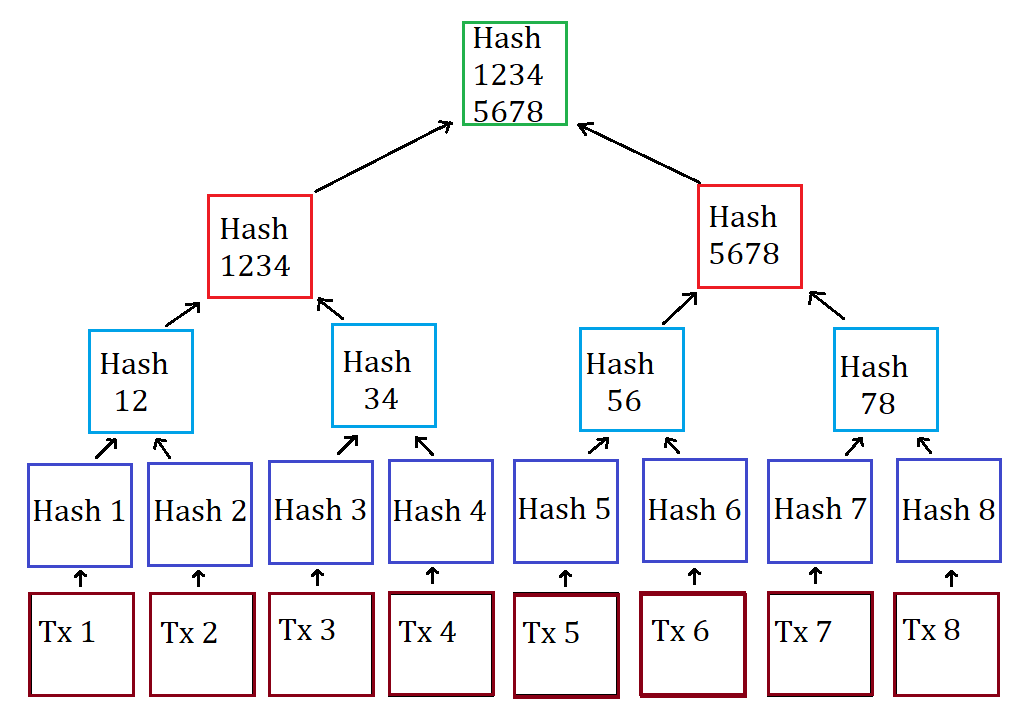
\includegraphics[width=\linewidth]{../src/img/Merkle_Tree.png}
  \caption{Merkle Tree example consisting of 8 underlying transactions.}
  \end{figure}
\item
  \textbf{Patricia Tree}

  A Patricia tree (aka prefix free radix tree) is a different data
  structure where the \texttt{(key,\ value)} pairs that are contained
  within it have the values at the leaf nodes, and the keys let you
  traverse a path from the root of the tree to the leaves, so that the
  nodes that share the same prefix in the key also share the same path
  down the tree from the root to the leaves.

  \begin{figure}
  \centering
  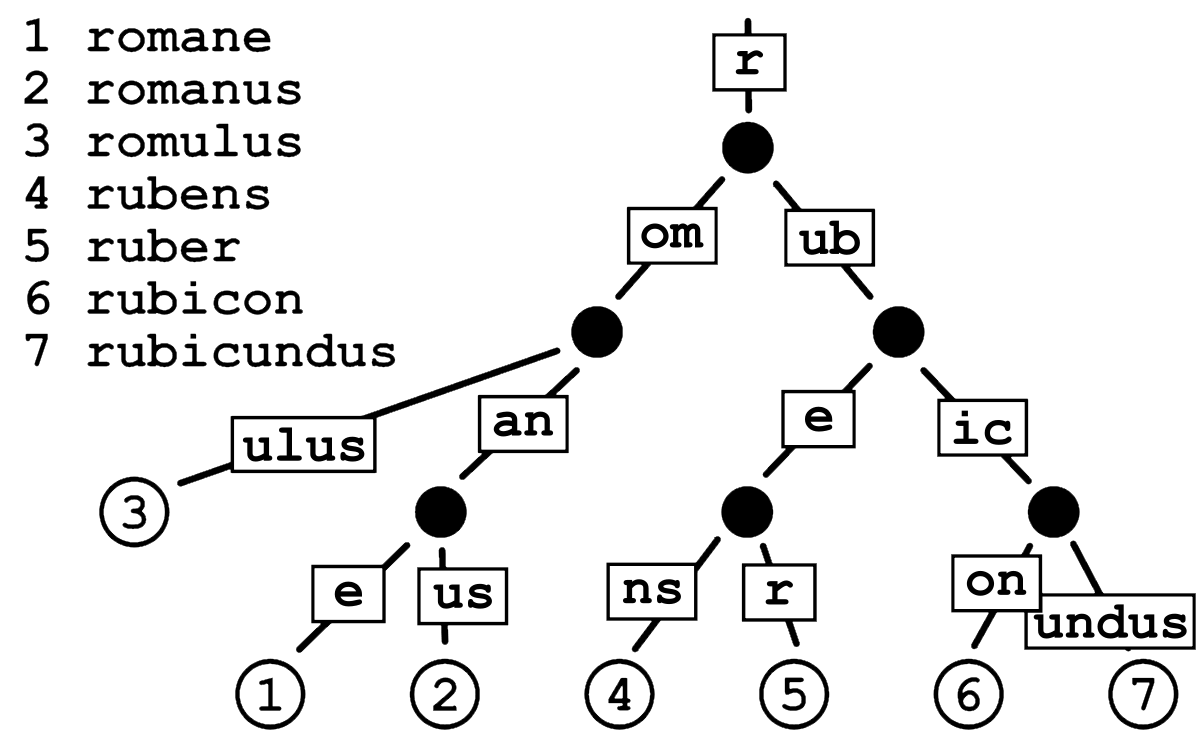
\includegraphics[width=\linewidth]{../src/img/Patricia_Tree.png}
  \caption{Patricia Tree Example}
  \end{figure}

  Ethereum uses a modified combination of a Merkle tree and Patricia
  tree that specifically suits the Ethereum data structures. In this
  particular case, it uses a Hexane-Merkel-Patricia tree which means
  that each node has 16 children. There's also a recent proposal to
  convert this to a binary tree.
\item
  \textbf{Other data structures}

  When looking at the programming languages supported on Ethereum, let's
  take for example \texttt{Solidity}, there are many common data
  structures such as arrays, lists, the basic value types, reference
  types\ldots{}
\end{itemize}

\subsection{Consensus Algorithm}\label{consensus-algorithm}

One of the critical core compontents (perhaps the most critical one) is
the consensus algorithm.

\begin{itemize}
\item
  \textbf{Why is there a need for a consensus algorithm this?}

  The Ethereum blockchain, as mentioned earlier, consists in many
  peer-to-peer nodes: these nodes are all talking to each other and
  trying to agree upon what is the global state of the blockchain.\\

  Each of the nodes has a local state, which consits on new blocks being
  formed containing the transactions that are processed by the node. But
  then, everyone on the Ethereum blockchain should agree upon what is
  the one canonical blockchain that will be used in the future.\\

  This is agreement is reached through the \textbf{consensus algorithm}.
  Decentralized consensus is critical to any blockchain. In the context
  of Ethereum it refers to the \textbf{Nakamoto Consensus Protocol} that
  is adapted from Bitcoin. This protocol addresses the problem of which
  miners' block should be included next to create the canonical
  blockchain. There are two components to this: \textbf{Proof of Work}
  (PoW) and \textbf{The longest chain rule}.\\

  PoW is used to determine which entity on the Ethereum blockchain gets
  to add the next block; \textbf{the consensus algorithm} determines
  which is the longest chain so far, and all the nodes that are chosen
  to add the next block to the existing canonical blockchain build upon
  the existing longest chain. This is how a blockchain grows in state.\\

  The consensus algorithm is used as a form of \textbf{sybil resistance}
  mechanism. There's this concept of 51\% attack, which consists in the
  scenario of 51\% of the participating entities colluding. Then, these
  malicious entities can change past states (and thus the state
  transitions) that have been encoded into the blockchain. This breaks
  the key property of immutability of a blockchain, thus it is very
  critical.
\end{itemize}

\subsection{Ethereum PoW: Present and
Future}\label{ethereum-pow-present-and-future}

As mentioned previously, Ethereum Proof of Work is fundamental to how
the Ethereum consensus protocol works. Technically, it is referred to as
Ethash, and it's formally defined as

\begin{align*}
(m,n)&=\text{PoW}\left(H_{\stkout{n}},H_n,d\right)\\ m&=H_m\wedge n\leq\frac{2^{256}}{H_d}
\end{align*}

where $H_\stkout{n}$ is the new block's header but without the nonce ($n$)
and mix-hash ($m$) components; $H_n$ is the nonce of the header;
$d$ is a large data set needed to compute the mixHash and $H_d$ is
the new block's difficulty value.

What a miner has to do is to determine a combination of mix-hash $m$
and nonce $n$ for every block to satisfy the constraint on the
difficulty for that particular block. This is a trial and error process
so the miner has to keep repeating the computation until a combination
of $m$ and $n$ that satisfies the difficulty is found. When this is
done it means that a sufficient amount of work has been performed by the
miner for this particular block, or in other words this indicates that
there is proof of work by the miner for this block.

PoW is being replaced by what is known as \textbf{proof of stake} (PoS)
with \textbf{the merge}. This change is important from a security
perspective: the consensus algorithm is critical to the economic
security of a blockchain, as it is what makes the blockchain resistant
to attacks from any of the untrusted parties operating the
infrastructure or operating on it. For now, this security is provided by
PoW.

\subsection{\texorpdfstring{Ethereum protocol upgrades (initially
\texttt{Eth2})}{Ethereum protocol upgrades (initially Eth2)}}\label{ethereum-protocol-upgrades-initially-eth2}

\textbf{The merge} the first of a set of interconnected upgrades to the
existing Ethereum network that are being made, perhaps the biggest set
of upgrades since Ethereum started. Although it was initially coined as
\texttt{Eth2}, this name was phased out because it is not a separate
version of the protocol but a continuation of all the research and
development activity that has happened on the protocol. These upgrades
occur across three vectors: \textbf{scalability}, \textbf{security} and
\textbf{sustainability}.

\begin{itemize}
\item
  \textbf{Scalability}: made possible by the concept of sharding.\\
\item
  \textbf{Security}: through the transition from PoW to proof of stake
  (PoS), also known as the merge.

  This is again a huge change to how the protocol functions and it
  offers immense economic and security benefits compared to PoW.\\
\item
  \textbf{Sustainability}: with PoW, there's a certain amount of
  computation that has to be done to pass the difficulty level. This is
  for sybil resistance part of the consensus protocol.\\

  As a result, there is real energy (in terms of running the mining
  nodes) that is consumed. This goes away to a great extent when we
  transition to PoS: it is going to make Ethereum much more sustainable
  when it comes to environmental impact.
\end{itemize}

These upgrades already started happening with the deployment of the
Beacon chain and the transition to PoS with the merge.

\subsection{Ethereum Nodes and
Clients}\label{ethereum-nodes-and-clients}

An Ethereum node is a software application that implements the Ethereum
protocol specification. It communicates with other Ethereum nodes on the
network in a peer-to-peer fashion.

The Ethereum client is a specific implementation of the Ethereum Node.
Within the Ethereum clients, a specification of the protocol itself (the
consensus algorithms, data structures,\dots all these core components)
is implemented.

If anyone is running an Ethereum node they're using one of these
Ethereum clients that have been built by multiple teams around the
world. The most popular ones are

\begin{itemize}
\tightlist
\item
  Geth
\item
  Erigon
\item
  Nethermind
\item
  OpenEthereum
\item
  Reth
\end{itemize}

There have been a lot of transitions and changes. Some of the clients
have been under development, and some of them are way more popular. Geth
is the most popular with more than 80\% of the running nodes. But, for
the sake of the diversity and decentralization of Ethereum, other
clients are being supported and being developed as well. These clients
are open source so anyone is free to examine the client code and maybe
even contribute to it.

Ethereum transactions are sent to the Ethereum Nodes, and these in turn
broadcast them across the peer-to-peer network. This is how Ethereum
transactions propagate across the Ethereum network, reach the various
nodes, get combined into blocks and result in the blockchain.

\subsection{Ethereum Miners}\label{ethereum-miners}

Ethereum miners are entities running Ethereum Nodes on the network. They
are the ones that receive, validate, execute and combine the
transactions into blocks.

They also provide a mathematical proof of their computation (proof of
work; PoW). For all this work, if the miner's block gets chosen to be
part of the blockchain, then they are rewarded with what is known as a
block reward.

This block reward is currently 2 Ether and it has decreased over time.
This is the crypto economics: incentive for miners to participate and to
be honest on the Ethereum network. Along with this reward, they're also
rewarded with transaction fees: the Ether spent on Gas by all the
transactions included in that block.

So block reward and transaction fees are the crypto economic incentives
that are paid out to the miner whose block gets accepted into the
blockchain.

\subsection{GHOST protocol}\label{ghost-protocol}

So transactions are sent, and miners validate them. They combine them
into blocks and these blocks are propagated over the peer-to-peer
network. Multiple miners are doing this process simultaneously. This
leads to multiple valid blocks at any level of the blockchain. The
canonical blockchain needs to choose one valid block at any level. The
choice of that valid block is dictated by the ``\emph{\textbf{GHOST
protocol}}'' (the Greedy Heaviest Observed Subtree protocol). This
protocol allows stale blocks up to seven levels in this calculation.
Stale blocks, in Ethereum's nomenclature, are referred to as uncles or
armors.

\section{Gas Metering: Solving the Halting
Problem}\label{gas-metering-solving-the-halting-problem}

\subsection{The Halting Problem}\label{the-halting-problem}

We talked earlier about Turing completeness and how Ethereum supports a
Turing complete programming language.

Turing completeness lends itself to a fundamental problem in computer
science: the halting problem. Imagine you have a Turing complete
programming language, then the halting problem states that: it cannot be
predicted if an arbitrary program in that language with an arbitrary
input will ever stop execution for that input.

This problem is taken for granted on our personal laptops or on our
phones: if there are programs that run into an infinite loop that hangs
them, then we just manually kill the execution.

In the context of a blockchain however, we are talking about being able
to deploy a smart contract that is not going to run on my Ethereum node
exclusively, but it's going to run on all the Ethereum nodes in the
blockchain. With that in mind, if any of those smart contracts ran into
an infinite loop, then the whole infrastructure would come to a grinding
heart, which is obviously undesirable. We would not make further
progress and everything would come to a standstill.

The way in which Ethereum deals with this issue is constraining the
resources that are given to the smart contract on the Ethereum node by
metering them through the concept of Gas.

\subsection{Gas Metering}\label{gas-metering}

The EVM runs smart contracts, which have machine code instructions.
Every single one of these instructions has a predetermined execution
cost in Gas units. So when a transaction triggers the execution of that
smart contract, and the smart contracts starts executing those
instructions, then the Gas units for those instructions are ``consumed''
by the smart contract. This is the concept of Gas metering within a
smart contract, where it accounts for every instruction (it could be a
computational instruction, a data access, \ldots{} all those
instructions consume Gas units from the transaction).

This implies that a transaction that triggers a smart contract has to
include a specific amount of Gas as required by the logic of the smart
contract. Depending on what logic needs to be executed by said smart
contract, there is a limit to the gas: a certain amount of Gas units are
required for a particular flow, so if a transaction is triggering that
it must include so many Gas units. In fact, even if the transaction is
just triggering a transfer of value, it has to supply the amount of Gas
required for what it is triggering.

If the Gas that is required during the execution of the smart contract
exceeds what is supplied, or if it exceeds the limit, then the EVM will
terminate execution and the transaction will fail. This is fundamental
to how Ethereum works, since there is a need to bound the use of
resources by anyone interacting with a smart contract that runs on all
the blockchain nodes all over the world.

Up until this point, all we have talked about is the units of Gas that
have to be provided. However, Gas itself has a price, which is measured
in Ether. So this Gas price is not fixed as it depends on the supply and
demand of Ether.

In this context it depends on the demand for the block space within
Ethereum, and if there are many applications (many smart contracts)
and/or users competing for that block space, then the Gas price can
increase vastly. So just like the automobile analogy (which requires Gas
or petrol, and with a fixed amount of petrol one can drive a certain
amount of kilometers), the petrol is the equivalent of the Gas units in
Ethereum (which allows to run a transaction in a certain number of
instructions within the smart contract based on the amount of Gas you
supplied). But the Gas price, similar to the price that you pay in Gas
stations (petrol bunks) is different and depends on the supply and
demand.

This Gas mechanism has recently been updated; take a look at EIP1559
(Ethereum Improvement Proposal 1559).

The take home message for this section is: one needs to obtain gas,
which is obtained by purchasing Ether. A transaction requires gas, and
if it exceeds the amount of Gas that is supplied, then the transaction
fails. But if there is more Gas than what is required, that is supplied
as part of the transaction, then the remaining Gas is sent back to the
sender who executed the transaction as part of the protocol.

\section{web2 vs.~web3: The Paradigm
Shift}\label{web2-vs.-web3-the-paradigm-shift}

In this section, we are going to assume that you are familiar to some
extent with web2 and most of the content will be focused on web3 and the
differences with web2.

\subsection{Objectives of web3}\label{objectives-of-web3}

The idea of web3 is for it to be a permissionless, trust minimized and
censorship resistant network for transfer of not only information but
also value.

Privacy and anonymity are again very big motivating factors in web3 and
have a huge implication on how we think about security in this space and
how we can actually conceive implementing various security measures.
However it isn't a completely fresh start: there are a lot of web2
security principles, best practices and software engineering best
practices that have been researched, experimented, developed and refined
over the last 3 or 4 decades that still apply very much to web3.

In the web3 world the aspirational goal is that of borderless,
permissionless innovation and censorship resistance. This inspires all
the applications, smart contracts or any other off-chain components to
be open and composable by design.

Composability means designing components and applications in a modular
way, so that other modules (or other applications) can interface with
them to increase the utility that is got from either of the two
components. This has to be done in a way that is very easy,
permissionless and effortless. Again, going back to the web2 space, a
lot of the work that has happened, a lot of the applications that are
built by the various enterprises, for various reasons such as protecting
their business interests, are designed in such a way that they work well
within their ecosystem or their suite of products, and they're not
really meant to be very composable or very interactive with other
applications or other components from other entities or other vendors
(potentially their competitors).

In the web3 world the aspirational goal is that of borderless,
permissionless innovation and censorship resistance. This inspires all
the applications, smart contracts or any other off-chain components to
be open and composable by design. This means that anybody (any user, any
part of the world) can deploy applications and interact with it (be it
contracts, be it any other component). This drives innovation in the
web3 space, which is great and has resulted in a very accelerated
innovation and compressed time. Again this has implications to to how
security is thought of and what is practically possible with security in
this space. When you have this unconstrained composability, where any
smart contract, any application that is deployed can be acted upon and
be combined or connected with any other smart contract on the chain,
then it leads to sort of an explosion of the dependencies and
configurations that are possible. This makes characterizing web3
vulnerabilities and exploit scenarios very challenging, because it
requires really a very deep knowledge of all these interacting
composable components along with their very different constraints that
could change because of composability itself, and their configurations
could be affected by interactions with other components.

Having said that, there are still many aspects of web3 security which
are really a paradigm shift.

\subsection{Open-source \& Transparency}\label{open-source-transparency}

Due to web3's ethos (or the design approach) towards everything here
being open source and transparent, the way it is thought about the
security of the ecosystem has to be changed.

We have known open source in the web2 world for several decades, so
that's not very new. But from an approach perspective, in the web2 space
we do see most of the products, or many of the products, being
proprietary from a licensing and from a source code availability
perspective. The web3 ethos stems from the permissionless aspect, the
trust minimization aspect and the censorship resistance aspect.

In the context of smart contracts, they're again expected to be open
sourced and also expected to be verified contracts. In this case it
means that the bytecode (machine instructions) of the contracts deployed
on the blockchain are expected to be source code verified using one of
the services available (such as
\href{https://etherscan.io/}{Etherscan}). This means that the source
code of the contract is the same one that was compiled, deployed and
that users interact with. That verification is something critical and
expected by default in this space.

Remember that everything that happens in the blockchain is transparent;
anyone can actually run an Ethereum node so that you don't even have to
rely on a block explorer or any service like that (more on that in
upcoming secitons). You can look at transactions as they happen in real
time on the blockchain, you can also look at transactions that are
waiting to get into the blockchain (through mempool explorers). One can
even do that by running an Ethereum node themselves. \textbf{There is no
security by obscurity}.

\subsection{Code Immutability}\label{code-immutability}

In the context of a blockchain being immutable (because of all the
blocks being linked with hashes), PoW and what it requires for somebody
to go back in time and change one of the blocks or any of its contents,
which contributes to the economic security and the immutability aspect
of the blockchain.

When it comes to code, the contracts that are deployed on the Ethereum
blockchain are designed in a way to be immutable as well. This means
that once a contract code is deployed, it is technically considered
immutable: it cannot be changed (at least in theory). There are some
exceptions, so theoretically it can done, but from a design perspective
(from an ethos perspective) this is not desirable. This code
immutability affects the way in which security is handled.

As it is already widely known, software will have bugs: one cannot prove
the absence of bugs, or the absence of vulnerabilities or errors in a
piece of software. Immutability affects this to a great extent: we know
that bugs will exist and, if you cannot change the contracts, then how
do we fix the code and redeploy the fixed code as we've been used to in
the web2 world (where we keep getting updates to the operating system or
to the different apps continuously to fix bugs, optimizations and so
on)?

This is something very fundamental to Ethereum or the web3 space that we
have to keep in mind.

There are practical exceptions: the deployed contract can be modified:
the functionality can be modified. This can be done in three ways:

\begin{enumerate}
\def\labelenumi{\arabic{enumi}.}
\item
  The contract can be modified and redeployed at a new address, but then
  you would have to carry over all the state. And all the users
  interacting would have to migrate to interacting with the new
  address.\\

  This is typically considered impractical but it can theoretically be
  done.
\item
  The modified contract (after bugfix or a version 2) can also be
  redeployed as a new implementation of what is known as a proxy
  pattern: the proxy contract points to an implementation contract, and
  that implementation can be modified.\\

  This is the most commonly used approach to contract upgrading, and
  again this has huge security applications if it is not done right, if
  it is not done in a trustworthy manner or if there are certain best
  practices that are not followed.
\item
  Using the \texttt{CREATE2} opcode, it allows updating a contract in
  place at the same address using the same unit code that was used to
  initialize the contract.
\end{enumerate}

We are going to further elaborate on the concepts briefly mentioned here
on upcoming sections.

\subsection{Client-Server
vs.~Peer-to-Peer}\label{client-server-vs.-peer-to-peer}

The pivotal difference between web2 and web3 is their underlying
paradigm.

\textbf{web2} relies on the \textbf{client-server paradigm}: we are used
to employ cloud services that have servers running, which we interact
with using our clients (laptops, phones, smart watches\dots) that are
\textbf{centrally managed}, i.e.~you have all these corporate entities
that determine what the infrastructure is, what the products are and
what the next versions of the products will be.

Applications are centrally rolled out and the consumers use them, but
they do not have a say in how the infrastructure is managed or how the
applications evolve. Sometimes, users don't even have a say as to what
kinds of applications can be deployed on the infrastructure: there is a
latent \textbf{censorship on web2}.

The former scenario is something that web3 is trying to get away from:
it's trying to go back to the original vision of the web which was for
it to be completely peer-to-peer without centralized entities that can
dictate what can be done on the platform, what can be deployed or who
can use it.

The idea is employing peer-to-peer communication not only for computing
power but also for storage and network, which are the building blocks of
web3. In the case of Ethereum, the peer-to-peer infrastructure that
supports these components is known as the \textbf{Ethereum triad}:

\begin{itemize}
\tightlist
\item
  \textbf{Coputing power}: Ethereum itself; Ethereum as a blockchain is
  used for decentralized compute.
\item
  \textbf{Storage}: Swarm.
\item
  \textbf{Network}: Whisper (now known as Waku).
\end{itemize}

\subsection{Business models}\label{business-models}

web2 business models are built around \textbf{freemium models} where the
basic application is free but if you want to upgrade, you have to pay
up. A lot of the business models (Google, Facebook especially) are built
around advertising, where the product is free.

In some sense, the user becomes the product and the interactions (the
data that the user shares with those platforms) is monetized in the form
of advertisements that are being delivered to the user. This is
something that we've just got used to and we don't even pay attention to
anymore.

In web3, since everything is decentralized, there has to be some
incentive for users to deploy the nodes and to contribute to the
development of the code, clients, smart contracts and applications. This
is driven by what is known as ``\emph{incentivized participation}'',
which goes back to the concept of crypto economics. This has big
implications to how security works because there is no real centralized
entity that can deal, manage and do instant response.

\subsection{Programming languages}\label{programming-languages}

Programming languages are critical because they are the means of how
projects implement their ideas, deploy them and let users interface with
them.

Again, programming languages are fundamental to the security of any
product, any architecture if you will. In the case of web2 there have
been numerous programming languages, being some of them way more popular
than the rest: it started with \texttt{C} and \texttt{C++} during the
Unix days 30 or 40 years ago, and since then we have seen different
declarative languages, subject-oriented languages and scripting
languages. Some of the most popular ones have been \texttt{Javascript}
and more recently \texttt{Go}, \texttt{Rust} and even some unique
languages such as \texttt{Nim}, that have been used to implement
Ethereum 2.0 clients recently.

All those languages are still applicable to the web3 space, because web3
is a combination of smart contracts that run on the blockchain and web
interface component (which is how users interact with the contracts on
the blockchain).

When it comes to the web component, all the web2 languages are relevant.
A lot of them are popular even here in terms of the interface, but also
in terms of the tooling that is used for the development of smart
contracts themselves.

Smart contracts themselves have a special language. In the case of
Ethereum, that's \texttt{Solidity}: it is the most widely used language
for writing smart contracts on Ethereum. There are others, like
\texttt{Vyper}, that are gaining traction, but for the majority of the
smart contracts that we see deployed, \texttt{Solidity} is that
language.

The smart contract languages were created specifically for web3, and
specifically for Ethereum in this case. So the security features of
those languages have obviously huge implications to the security of the
smart contracts themselves and the applications that are built on top of
them.

\subsection{Applications in web3:
ÐApps}\label{applications-in-web3-uxf0apps}

Building applications on a decentralized infrastructure (i.e.~a
blockchain) will cause such applications to be fundamentally different
from the mobile applications or the desktop applications that we are
used to today (as we can already guess by looking at the programming
languages and code immutability in web3). These applications are
referred to popularly as decentralized application or ÐApp.

These applications rely on a concept that is very unique to web3:
\textbf{on-chain} and \textbf{off-chain}.

\begin{itemize}
\tightlist
\item
  \textbf{On-chain} means something that is running or executing on the
  blockchain or within the blockchain's execution environment.
\item
  \textbf{Off-chain} is something that is running outside the
  blockchain.
\end{itemize}

In the web2 space everything is off-chain because, obviously, there is
no concept of blockchain. However, in order to function, the web3 space
makes use of an off-chain component combined with an on-chain component.

The off-chain component is all the web2 or ``\emph{the glue}'' that
binds the web interface to the smart contracts that are running
on-chain. This distinction is critical when thinking about security.

To put it simple, a ÐApp combines a web app/web front-end or a mobile
app (the off-chain component) that interacts with a smart contract on
the blockchain (the peer-to-peer infrastructure which is a combination
of compute, storage and network; the on-chain component). In many cases
we have one or more of any of the mentioned.

In the case of Ethereum, what is peer-to-peer is the compute part and
the peer-to-peer storage aspects (such as IPFs and some of the other
protocols that we won't talk about).

The security of web3 has to think about the security implications of
anything running or interacting off-chain with that running on-chain as
well. It's not just smart contract security but also the security of the
off-chain web or mobile app components that interface with the on-chain
components (the smart contracts).

The main difference however between web2 and web3 security is the
on-chain component of course. We will need to think about at the
pitfalls that are unique to smart contracts and look at the best
practices.

\subsection{Unstoppability \&
Immutability}\label{unstoppability-immutability}

Another difference between web2 and web3 is that the web3 applications
and infrastructure are unstoppable and immutable.

We talked about ÐApps and how they run on a decentralized
infrastructure. The goal is even for the governance of these protocols
and infrastructure to be decentralized, this means that there is no
single entity that can unilaterally decide to make changes, to start
something, to stop the application (be it adapt be the protocol, be the
surrounding infrastructure or the governance itself). Specifically, in
the case of smart contracts, there shouldn't be a single entity.

This could be the the project team itself that has built out this
application or the contracts: they shouldn't be unilaterally allowed to
change, stop and withdraw funds. This stems from the trust minimization
motivation and the censorship resistance aspect.

They are all very interconnected aspects and as you can imagine they
have huge implications to when it comes to upgrading the contracts,
fixing the bugs or doing anything with the smart contracts once they're
deployed; because they are expected in theory, by motivation and by
design (codewise; remember the code immutability we talked about
earlier) to be unstoppable and immutable.

From a security perspective, this makes it hard to deploy the software
because once you do it, if there are any vulnerabilities found, it's
very hard to do an instant response (just what we talked about on code
immutability). The latter is something we take for granted in the web2
world, where we get software updates even without our knowledge.

In the case of web3, and particularly Ethereum smart contracts, this has
huge implications to how we think about design and operationalize
security. This is the ultimate goal, in practice, as we go through
different stages of progressive decentralization.

These things are evolving, so the best practice right now is to do
something known as a ``\emph{guarded launch}'' (basically initially
limiting the functionality of the ÐApp for monitorization purposes). For
now the best practice is to have the ability to make changes, to upgrade
the contracts, to have an emergency withdrawal function, to remove the
tokens in case there is an emergency. It's sort of the stop cap measure
as we progress towards complete decentralization.

Once we have enough confidence that the contracts are running and there
are no bugs, vulnerabilities or exploits, then a lot of these things are
disabled in the code: the kill switches or the credibility aspects the
governance\ldots{}

All these things are in a progressive manner made more decentralized
over time.

\section{Decentralization}\label{decentralization}

\begin{itemize}
\tightlist
\item
  \textbf{What does decentralization really mean?}
\end{itemize}

This term is used very casually although it has huge implications to how
we think about security, even for smart contracts. There is a definition
put forth by Vitalik in his article on decentralization. There are three
types of decentralization:

\begin{itemize}
\item
  \textbf{Architectural decentralization}: it refers to the hardware
  (the physical computers); who runs them, owns them, who is managing
  them, who can start them and stop them. This can be done in a
  decentralized fashion or not.
\item
  \textbf{Political decentralization}: it refers to the people behind
  the hardware or what is commonly referred to as ``\emph{wet ware}''.
  Who are the individuals or the organizations who control the hardware
  or the infrastructure? Is it just one individual or is it a group of
  individuals? Are the colluding or are they independent and
  decentralized?
\item
  \textbf{Logical decentralization}: it refers to the software: used to
  build out the applications (the framework itself, the Ethereum code,
  the protocol itself, the data structures in it, the smart contracts or
  any other software that runs in that stack). Is that decentralized? Is
  it a monolithic entity that cannot be split apart and used in a
  decentralized fashion?
\end{itemize}

All of these have security implications.

\section{Cryptography, Digital Signature and
Keys}\label{cryptography-digital-signature-and-keys}

Most of you know tat there are two classes of cryptography:

\begin{itemize}
\tightlist
\item
  \textbf{symmetric cryptography}: there is a single key shared between
  parties.
\item
  \textbf{asymmetric cryptography}: there is a key pair; public key and
  private key.
\end{itemize}

In the case of Ethereum, the cryptography that is used is all about
digital signatures and not as much about encryption at a protocol level.
These digital signatures however depend on the concept of public key and
private key.

\subsection{Private Key}\label{private-key}

The private key is a secret and the owner has to keep it in a safe
place. In the case of Ethereum, it's a 256 bit private key. It's
effectively a random number and it's used to derive the public key.

\subsection{Public Key}\label{public-key}

The public key, however, is not secret. It is a point on the elliptic
curve calculated from the private key using elliptic curve
multiplication. The public key is used then to derive the address of an
Ethereum account (by hashing the public key by means of the keccak-256
cryptographic hash function and taking the last 20 bytes of the output;
it is a very simple calculation) and it is also used by others to engage
in cryptographic protocols with the owner of the private key.

It is important to remember that the public key cannot be used to derive
the private key. This is should be something obvious to security,
because otherwise if the public key could be used to derive the private
key, then this key pair system would not deliver any kind of security.

This is the high-level aspect that you need to remember: there's a
private key, which is used to obtain the public key, and from the public
key we derive the address of the Ethereum account.

\subsection{keccak-256}\label{keccak-256}

We mentioned earlier that the keccak-256 cryptographic hash function is
used in the steps of computing the EOA address from the public key.

keccak-256 is actually the cryptographic hash function that is used by
Ethereum. It is very closely related to the SHA3 (the secure hash
function). The latter was finalized as the standard by MIST (National
Institute of Standards and Technology) and in the case of Keccak-256, it
was the winning candidate for the SHA3. However, the SHA3 standard was
adopted instead (because some minor modifications were applied).

keccak-256 is critical to a lot of the functioning of the Ethereum
protocol and smart contracts as it's a fundamental primitive to how
computation in many ways is done on Ethereum.

\subsection{Digital Signature: ECDSA}\label{digital-signature-ecdsa}

The digital signature algorithm used by Ethereum is the same one that is
used by Bitcoin. It is known as ECDSA: \textbf{Elliptic Curve Digital
Signature Algorithm}.

Elliptic Curve Cryptography is an approach to public key cryptography
based on a particular algebraic structure of elliptic curves over finite
fields.

In the case of Ethereum, the particular elliptic curve used is known as
Secp-256k1 (this refers to the parameters that are used for the elliptic
curve).

Digital signatures are fundamental to how Ethereum works, are powered by
public key cryptography (asymmetric cryptography) and have three main
purposes:

\begin{enumerate}
\def\labelenumi{\arabic{enumi}.}
\tightlist
\item
  \textbf{Authorization}: inclusion of the signature proves that the
  owner of the private key who created the signature (and who by
  implication is the owner of the sending Ethereum account) has
  authorized the transaction to spend the ether or to execute the
  contract that it is targeted.
\item
  \textbf{Non-repudiation}: once the signature has been included, it
  cannot be later denied that authorization was granted for that
  transaction to execute.
\item
  \textbf{Integrity}: it proves that the transaction data has not been
  modified or cannot be modified by anyone after the transaction has
  been signed. This is one of the fundamental security properties.
\end{enumerate}

\section{Ethereum State \& Account
Types}\label{ethereum-state-account-types}

Ethereum state is a mapping from the address of the Ethereum accounts to
the state contained within it as a data structure. It is implemented as
a \textbf{Modified Merkle-Patricia Tree}: a combination of a Merkle tree
and a Patricia tree with some changes that are specific to Ethereum.

Each of the Ethereum accounts has a unique 20 byte address associated
with it, which is used by accounts to ``talk to each other''. Addresses
are critical to how messaging works within the Ethereum protocol and how
the accounts engage in transfer of value or information, since accounts
need to be able to refer to each other using their addresses.

In addition, accounts have four fields:

\begin{itemize}
\tightlist
\item
  \texttt{nonce}: a counter that's used to make sure that each
  transaction can only be processed once used to prevent replay attacks.
\item
  \texttt{balance}: a number representing the amount of Ether that the
  account has at any point in time.
\item
  \texttt{code}: the smart contract code (absent in Externally Owned
  Accounts).
\item
  \texttt{storage}: the associated smart contract storage (absent in
  Externally Owned Accounts).
\end{itemize}

\subsection{Account types}\label{account-types}

Ethereum has two account types:

\begin{itemize}
\item
  \textbf{Externally Owned Account (EOA)}: it is an account that is
  controlled by a private key.\\

  Anyone who has a private key can create a digital signature that can
  be used to control the Ether that is present in an EOA. These
  signatures can be used to sign transactions from the EOA, which in
  turn can trigger messages from the EOA to other accounts.\\

  These messages can result in a transfer of value or they can trigger
  smart contracts. An EOA does not have any associated code or storage.
\item
  \textbf{Contract account}: it is an account that is controlled by the
  code that is contained within that account.\\

  Unlike EOAs, contract accounts have an associated smart contract code
  and storage. Whenever the contract account receives a message, it
  triggers the code present and accesses any internal storage associated
  with it. When the code runs it can send messages to other accounts or
  even create new contracts.
\end{itemize}

In this sense, smart contracts can be thought of autonomous agents as
they're always present in the execution environment of the Ethereum
blockchain. They're always ready to be triggered by a transaction or a
message that is sent to them.

Through their contract account they have access to the Ether balance and
the contract storage. The execution of the code results in manipulation
of this balance and the contract storage.

\section{Transactions: Properties \&
Components}\label{transactions-properties-components}

Transactions are \textbf{signed messages} that originate outside of the
Ethereum blockchain. They are \textbf{triggered by EOA}s (that are
managed or controlled by a private key). The trigger happens to be the
digital signature, derived from the private key.

These transactions are transmitted by the Ethereum network and they
trigger state changes on the blockchain. In fact, Ethereum is
fundamentally a transaction based state machine, as only transactions
are capable of triggering state changes.

\subsection{Properties}\label{properties}

\begin{enumerate}
\def\labelenumi{\arabic{enumi}.}
\item
  Transactions are \textbf{atomic}: they run from the beginning to the
  end completely, it's either all or nothing.\\

  So the side effects of the transactions are only reflected in the
  blockchain if they run to completion. If they don't, nothing that they
  do is reflected on the blockchain and it's as if the transaction never
  happened.\\

  In other words: transactions cannot be divided or interrupted with
  some of the partial state being reflected on the blockchain and the
  rest of it not.\\

  This contrasts withtraditional computing environments where a
  particular process or a particular control might be interrupted, gets
  context washed out and then something else (a different process or a
  thread) executes and then the original context is brought back. None
  of that happens within the context of Ethereum.
\item
  Transactions are \textbf{serial}: they're executed one after the
  other, sequentially without any overlapping. There is no parallelism
  when it comes to the execution of transactions.
\item
  Transaction \textbf{inclusion}. When a user submits a transaction,
  what is the warranty that it gets included within one of the blocks on
  the Ethereum blockchain?\\

  This property is controlled by entities on the Ethereum blockchain
  known as miners. They run Ethereum nodes and decide which transactions
  are included within a block. This depends on multiple factors, the key
  ones being the congestion on the Ethereum network (or in other words,
  the other transactions that are competing for the same block space)
  and the Gas price that the user decides to use for the particular
  transaction.
\item
  \textbf{Inclusion order}. It refers to the specific order of the
  transactions included within a block.\\

  Again, this chosen by the miners and, similarly to inclusion, is
  determined by factors of congestion and Gas price. The key takeaway of
  properties 3 and 4 is that there are entities known as miners on the
  blockchain who get to decide which transactions get included within a
  certain block and the specific order of the transactions within that
  block.
\end{enumerate}

\subsection{Components}\label{components}

Transactions contain seven components:

\begin{enumerate}
\def\labelenumi{\arabic{enumi}.}
\item
  \texttt{nonce}: the name is an abbreviation for ``a number used only
  once''. It's a sequence number that, as part of the protocol, is
  incremented in a particular fashion (it changes for every
  transaction).\\

  The application of the nonce is prevention of replay attacks
  (i.e.~replaying the same transaction over and over again). In the case
  of an EOA, the nonce value is equal to the number of transactions sent
  from that account. In the case of a contract, it is equal to the
  number of other contracts created by this contract account.
\item
  \texttt{gasPrice}: the price for every Gas unit that the sender is
  willing to pay for a particular transaction. It's measured in
  wei/gas.\\

  \texttt{gasPrice} is not fixed by the Ethereum protocol. The higher
  the Gas price that the the sender is willing to pay for this
  transaction, the faster the particular transaction gets included by
  the miner into a block in the blockchain. This price depends on the
  demand for the block space at the point in time when the transaction
  is submitted.\\

  The reason for this is that there is a limited amount of space in the
  block, so there's only a limited number of transactions (as determined
  by the Gas used by each one of them) that can be included within this
  block.
\item
  \texttt{gasLimit}: the maximum number of Gas units that the sender is
  willing to pay for a particular transaction. This depends on the type
  of transaction that is being sent.\\

  If it is a simple Ether transfer then it costs 21000 Gas units. But if
  it is a transaction that is targeting a particular contract (or a
  particular function of the contract) then the required amount of gas
  is higher. If sufficient Gas (in the form of Gas limit) is not set for
  the transaction (if it's less than what is required to), then it
  results in what is known as an \textbf{out of Gas exception} (OOG
  Error) and that transaction fails.\\

  The way it works is that for any transaction that is being sent by a
  sender, there is an estimated Gas that needs to be sent as part of the
  transaction. If that estimated amount of Gas is not sent then it leads
  to the exception. If there is excess gas, then the remaining Gas is
  sent back to the sender.
\item
  \texttt{recipient}: the destination 20 byte Ethereum address for a
  transaction (i.e.~the destination account that this transaction is
  targeting).\\

  This could be an EOA address or a contract address, it depends on the
  target of that particular transaction. It could be any address on the
  Ethereum blockchain, and the protocol itself does not validate these
  recipient addresses in the transactions. So one can send a transaction
  to any address and that address might not even have a corresponding
  private key, nor the contract that the sender expects to have.\\

  Thus, all such validation should be done at the user interface level.
  That validation is critical for security reasons (more on that in
  later chapters). Note that this recipient is really the target
  address. There is no ``from address'' that is a component of the
  transaction. The reason for this is that the ``from address'' can be
  derived from the ECDSA signature components $v$, $r$ and $s$:
  they can be used to derive the public key, which in turn can be used
  to derive said address.
\item
  \texttt{value}: the amount of Ether (in wei) that the sender is
  sending to the recipient address.\\

  What happens with such funds depends on the recipient: if it happens
  to be in EOA, then the balance of that account will be increased by
  this value and the sender's balance correspondingly decreases. If it
  hapens to be a contract account, then what happens depends on any
  other data present as part of this transaction (i.e.~the contract
  function being invoken with the transaction data).\\

  If there is no data being sent as part of this transaction, and the
  destination happens to be a contract account, then the contracts'
  \texttt{receive} or \texttt{fallback} functions (if they were defined
  or if they are present; more on that in the upcoming chapters) are
  triggered and thus, what happens with the received Ether depends on
  their implementation.\\

  If there is no \texttt{fallback} function, then the transaction
  results in an exception and the Ether, that is sent as part of the
  transaction, remains with the sender account.
\item
  \texttt{data}: payload of variable length and binary encoded (as per
  the format required by Ethereum) that is sent as part of this
  transaction.\\

  This field is relevant when the recipient is a contract account. As
  mentioned previously, the data in that case contains the contract
  function that is being targeted by the transaction plus the specific
  arguments that are relevant for said function.
\item
  \texttt{v}, \texttt{r} \& \texttt{s}: The ECDSA signature is 65 bytes
  in length and has three subcomponents: \texttt{v}, \texttt{r} and
  \texttt{s}.

  \begin{itemize}
  \tightlist
  \item
    \texttt{r} and \texttt{s} represent the signature components. They
    are 32 bytes in length each (adding up to 64 bytes).
  \item
    The final subcomponent, \texttt{v}, is the recovery identifier. It's
    just one byte and its value can be either 27 or 28, or it can be
    twice the value of chain ID ($2\times\text{ID}_\text{chain}$) plus
    either 35 or 36. The chain ID is the identifier of the blockchain.
    In the case of the Ethereum mainnet chain, $\text{ID}=1$.
  \end{itemize}
\end{enumerate}

For a particular transaction, the Ether used to purchase Gas is credited
to the beneficiary address that was specified in the block header (more
details on this are found in the upcoming sections). Then there's also a
concept of a Gas refund: the difference between the Gas limit and the
Gas Used is refunded back to the sender of the transaction. This is done
at the same Gas price as indicated in that transaction.

\section{Contract Creation}\label{contract-creation}

We mentioned that a transaction can result in contract creation.

The creation transaction is a special one because it's sent to a special
destination address called ``\emph{the zero address}'' (\texttt{0x0}
address), which is an address that has zero in all its bits. This zero
address is treated in a special maner within Ethereum, and it becomes
critical to some of the smart contract security properties.

It contains a data payload which represents the byte code of the
contract that is being created, and it may also contain an optional
Ether amount in the value field, in which case the new contract that is
being created, will have a starting balance equal to this Ether value.

\section{Transactions, Messages \&
Blockchain}\label{transactions-messages-blockchain}

\subsection{Distinction between Transactions and
Messages}\label{distinction-between-transactions-and-messages}

So far, we have used both the terms Transaction and Message
interchangeably, but in the context of the protocol they are actually
very different:

\begin{itemize}
\item
  \textbf{Transactions}: originate off chain (by an EOA when an external
  actor, that is, external to the blockchain, sends a signed data
  package onto the blockchain) and target an entity on the blockchain.\\

  This transaction can trigger a message that can do one of two things:

  \begin{itemize}
  \tightlist
  \item
    It can trigger a message to another EOA, in which case it leads to a
    transfer of value (transfer of Ether).
  \item
    It can trigger a message to a contract account, in which case it
    leads to the recipient contract account running its contract code
    and doing whatever the code is intended to do.
  \end{itemize}
\item
  \textbf{Messages}: the origination and the destination are both
  onchain\\

  Messages can be triggered in two ways:

  \begin{itemize}
  \tightlist
  \item
    externally by a transaction. The destination of that message could
    be another EOA or another contract account.
  \item
    internally within the EVM. This happens when a smart contract
    executes the call family of opcodes and that leads to the recipient
    contract account running its code, or value transfer to the
    recipient.
  \end{itemize}
\end{itemize}

\subsection{How to build a Blockchain}\label{how-to-build-a-blockchain}

Blocks are batches of transactions that are grouped together plus the
hash of the previous block (a cryptographic hash that is derived from
the previous flux data), creating thus a ``chain'' among the blocks.
This is how at high level a blockchain is constructed, and it is also
the fundamental reason why a blockchain is considered immutable, which
lends itself to the blockchain's integrity.

The reason for that is because if someone were to change any component
of a historical block (any of the transaction data: the destination or
any other aspect) then that change would affect all of the following
blocks: all the hashes that are included in the following blocks would
be different from the hash of the modified block, and this is something
that anybody running the blockchain or looking at the blockchain would
notice. That would break the the immutability of the blockchain.

To preserve the transaction history, blocks are ordered. Therefore,
every new block created contains a reference to its parent block and
similarly, transactions within the blocks are also strictly ordered. All
these critical aspects are the reason why the integrity of a blockchain
is maintained and prevents any fraud from happening.

\subsection{Block Header}\label{block-header}

So far we have said that the blocks in the Ethereum blockchain contain
transactions, but there's more to it: every block contains a block
header along with the transactions. The headers of the Ommer's blocks.

Each block header itself has several components to it that are critical
to how the Ethereum blockchain functions. They contain several things
such as:

\begin{itemize}
\item
  \textbf{The parent hash}: the hash of the parent block's header.\\

  This is what chains the blocks and the Ethereum blockchain together to
  make it immutable and provides the fantastic integrity property of the
  blockchain.
\item
  \textbf{The Ommer's hash}
\item
  \textbf{Beneficiary address}: the address of the Ethereum account to
  which the block reward for mining this block and all the transaction
  fees collected from the mining of the transactions included in this
  block are transferred to.\\

  This address is typically controlled by the miner who has mined this
  block.
\item
  \textbf{\texttt{stateRoot}}: one of the three root hashes of the
  modified Merkle-Patricia tree. These root hashes are 256 bit in
  length.\\

  The manner in which the state root is derived is critical to how the
  Ethereum state is captured within the blockchain: the leaves of the
  state root are \texttt{(key,\ value)} pairs of all the Ethereum
  address accounts.\\

  The keys are the Ethereum addresses of the accounts and the values
  represent the Ethereum state within that account.\\

  Recall that every Ethereum account has four fields: a \texttt{nonce},
  a \texttt{balance}, a \texttt{codeHash} and a \texttt{storageRoot}. If
  that account happens to be an EOA, then the \texttt{codeHash} and
  \texttt{storageRoot} don't really matter (they don't contain anything
  in them).\\

  But if that account happens to be a contact account, then the
  \texttt{codeHash} has the Keccak-256 hash of the code that is
  contained within that contract account, and the \texttt{storageRoot}
  of that contract account has the rootHash of another Merkle-Patricia
  tree where the leaves represent the storage that is associated with
  that contract.
\item
  \textbf{\texttt{transactionsRoot}}: one of the three root hashes of
  the modified Merkle-Patricia tree, where the leaves represent the
  transactions. Also 256 bit in length.
\item
  \textbf{\texttt{receiptsRoot}}: one of the three root hashes of the
  modified Merkle-Patricia tree, where the leaves represent the
  transaction receipts. Also 256 bit in length.\\

  \textbf{But what is a transaction receipt?}\\

  A transaction receipt can be thought of as the side effects of a
  particular transaction that are captured on the blockchain. Besides
  any changes to the account state that transactions might make, there
  are other side effects that are captured on the blockchain for this
  particular transaction. It is a tuple that contains four items:

  \begin{itemize}
  \tightlist
  \item
    \textbf{The cumulative Gas used}: the total Gas used in the block up
    until right after this particular transaction has happened, so in
    some sense it captures the ordering of the transactions within the
    block.
  \item
    A \textbf{set of logs}: related to the concept of events in
    \texttt{Solidity} (which we will study in the \texttt{Solidity}
    chapter). These are events that can be generated by any transaction
    that is captured on the blockchain.\\
    \strut \\
    They're really critical to how off-chan components, user interfaces
    and other components monitor what's happening with a smart contract.
  \item
    The \textbf{Bloom filters} specifically associated with those logs:
    they capture the indexed parameters for every event, so that one can
    query particular parameters of that event in a faster manner.
  \item
    A \emph{status quo}: what really happened with the transaction.
  \end{itemize}
\item
  \textbf{\texttt{logsBloom}}
\item
  \textbf{\texttt{dificulty}}: difficulty of the block in the context of
  PoW.
\item
  \textbf{\texttt{blockNumber}}: the number of blocks that have been
  mined so far right. This number sort of indicated the position of the
  block within the blockchain.
\item
  \textbf{\texttt{gasLimit}} (called Block Gas Limit under more formal
  contexts): the Gas limit that's specific to this block.\\

  This concept is essential to Ethereum as it dictates \textbf{the
  number of transactions that are added in this block}.\\

  This concept is different from the Gas limit which we talked about
  earlier that was specific to the transaction. This Block Gas Limit
  refers to the total Gas that is spent by all the transactions in that
  block and this effectively caps the number of transactions that can be
  included within that block.\\

  So the block size is in fact not fixed in terms of the number of
  transactions, but it's fixed in terms of the Gas used by all the
  transactions. The reason for that is that every transaction can
  consume a different amount of Gas.\\

  The Block Gas Limit is set by the Ethereum miners in a very
  interesting way: by voting on the blockchain. This is currently set to
  15 million and it has also changed over time, depending on the miners'
  voting. It also represents the level of demand there is for the block
  space on Ethereum.
\item
  \textbf{\texttt{gasUsed}}: the total Gas used by all the transactions
  in this block.
\item
  \textbf{\texttt{extraData}}
\item
  \textbf{\texttt{timestamp}}: (derived from the unix time) indicates at
  what point in time was the block was mined.
\item
  \textbf{mix-hash}: critical component of the PoW. See
  \textbf{subsection}
  \href{1.4_Ethereum_core_components.md\#Ethereum-PoW:-Present-and-Future}{\emph{\textbf{Ethereum
  PoW: Present and Future}}}.
\item
  \textbf{\texttt{nonce}}: critical component of the PoW. See
  \textbf{subsection}
  \href{1.4_Ethereum_core_components.md\#Ethereum-PoW:-Present-and-Future}{\emph{\textbf{Ethereum
  PoW: Present and Future}}}.
\end{itemize}

\section{EVM (Ethereum Virtual Machine) in
Depth}\label{evm-ethereum-virtual-machine-in-depth}

The EVM is the execution component of the Ethereum blockchain: it is the
runtime environment where all the smart contracts run. Recall that EVM
is a quasi-Turing complete machine: it's turing complete because the
underlying programming language supports arbitrary logic unbounded
complexity, but it's also bounded by the amount of Gas provided as part
of every transaction.

The Ethereum code runs within the EVM and it is written in a low level
stack based language referred to as the EVM Machine Code. This code
consists of a series of bytes (therefore referred to as a bytecode)
where every byte represents a single operation. So the opcodes are very
simple and each of them is a single byte.

\subsection{EVM Arquitecture}\label{evm-arquitecture}

Computer architectures are typically classified into either \textbf{von
Neumann architecture} or \textbf{Harvard architecture}. This depends on
how code and data are handled within the architecture: Are they stored
together? Are they transported over the buses together? How are they
cached? And so on\ldots{}

In the case of the EVM, the code is stored separately in a virtual ROM
and there is a special instruction to access the EVM code.

EVM is a very simple stack based architecture: the operands for EVM
instructions are placed on the stack and the output of those
instructions is also returned on the stack. There's no concept of
registers, virtual registers or anything like that.

Every architecture has a concept of a word and in the case of the EVM,
the word size is \textbf{256 bits}. It's believed that this was chosen
to facilitate some of the fundamental operations around the 256 hash
scheme and the elliptic curve computations.

The architecture is made up of four fundamental components:

\begin{enumerate}
\def\labelenumi{\arabic{enumi}.}
\item
  \textbf{The stack} The EVM has 1024 elements in the stack and each of
  those elements is 256 bits in length (equal to the word size). EVM
  instructions are allowed to operate with the top 16 stack elements.
  Most EVM instructions operate with the stack (because it's a stack
  based architecture) and there are also stack specific operations.
\item
  \textbf{The volatile memory}: in EVM, data placed in memory is not
  persistent across transactions on the blockchain. It is also linear
  (it's a byte array and therefore addressable at byte level) and zero
  initialized.\\

  There are three specific instructions that operate with memory, such
  as \texttt{MLOAD} which loads a word from memory and puts it onto the
  stack; \texttt{MSTORE} which stores a word in memory from the stack;
  and \texttt{MSTORE8} which stores a single byte in memory from the
  stack. These instructions (and more) will be reviewed in more detail
  in the following sections.
\item
  \textbf{The non-volatile storage}. Unlike memory, storage in EVM is
  non-volatile: data put in storage is persistent across transactions on
  the blockchain. It is implemented as a \texttt{(key,\ value)} store
  between 256 bit keys and 256 bit values, and it is also zero
  initialized.\\

  To understand how storage fits in within the concept of accounts and
  the blocks on the blockchain, recall that every account has a
  \texttt{storageRoot} field. This \texttt{storageRoot} field,
  implemented as a modified Merkle-Patricia tree, captures all the
  storage associated with that account. This is relevant for contract
  accounts that have associated storage. These \texttt{storageRoots}
  within the account are further captured as part of
  \texttt{the\ stateRoot}, which is one of the fields in the block
  header.\\

  There are two instructions that operate specifically on storage:
  \texttt{SLOAD} which loads a word from the storage and puts it onto
  the stack; and \texttt{SSTORE} which takes a word from the stack and
  puts it into storage.
\item
  \textbf{\texttt{Calldata}}: it is used specifically for data
  parameters of transactions and message calls. It is read only (it
  cannot be written to) and it's also bite addressable.\\

  There are three specific instructions that operate with call data:
  \texttt{CALLDATASIZE} which gives the size of the supplied call data
  and puts it onto the stack; \texttt{CALLDATALOAD} which loads the call
  data supplied onto the stack; and \texttt{CALLDATACOPY} that copies
  the supply call data to specific region of memory.
\end{enumerate}

\subsection{EVM Ordering}\label{evm-ordering}

Another concept typically associated with architectures is the concept
of ordering: \textbf{big-endian} ordering versus \textbf{little-endian
ordering}. In the case of the EVM, \textbf{it uses the big-endian
ordering}: the most significant byte of a word is stored at the smallest
memory address while the least significant byte is stored at the largest
address.

\subsection{Instruction Set}\label{instruction-set}

\emph{(A more complete and detailed description of the EVM opcodes can
be found in}
\href{https://www.evm.codes/?utm_source=tldrnewsletter}{\emph{evm.codes}}\emph{.
If there is any discrepancy/ambiguity of the contents found here, refer
to}
\href{https://www.evm.codes/?utm_source=tldrnewsletter}{\emph{evm.codes}}\emph{)}

Summarized walkthrough of the EVM opcodes

All the instructions supported by the EVM can be classified into 11
categories. Instructions that are found in categories \textbf{a} to
\textbf{i} operate on the stack.

The format for each of these instructions will be as follows:

\begin{lstlisting}[language=Solidity,numbers=none]
OPCODE MNEMONIC INPUTS OUTPUTS
\end{lstlisting}

\hfill\break
Let's see an example:\\

The opcode is the hex representation of the instruction. You will see
that the \texttt{0x00} opcode is used for the stop instruction. In
addition, the word \texttt{STOP} is the mnemonic of the instruction. and
then the two numbers that you see after the mnemonic refer to the number
of stack items placed for this instruction (inputs) and the number of
stack items removed (outputs).

So the stop opcode is \texttt{0x00}, thus it's the first instruction in
the instruction set mapping. The mnemonic is \texttt{STOP} (makes
sense), 0 items are placed and 0 items are removed from the stack.

In the case of \texttt{ADD}, you will see that it has 2 items placed
onto the stack (the 2 operands) and the computed result (the addition)
is placed back onto the stack.

That's why you see that there is one item placed onto the stack, which
is the result the addition of the two inputs. The same thing holds good
for multiplication, and so on\ldots{}

\hfill\break
\textbf{a. Stop \& Arithmetic}

\begin{lstlisting}[language=Solidity,numbers=none]
0x00 STOP 0 0
0x01 ADD 2 1
0x02 MUL 2 1
0x03 SUB 2 1
0x04 DIV 2 1
0x05 SDIV 2 1
0x06 MOD 2 1
0x07 SMOD 2 1
0x08 ADDMOD 3 1
0x06 MOD 2 1
0x07 SMOD 2 1
0x08 ADDMOD 3 1
0x09 MULMOD 3 1
0x0a EXP 2 1
0x0b SIGNEXTEND 2 1
\end{lstlisting}

\hfill\break
\textbf{b. Comparison \& Bitwise Logic}

\begin{lstlisting}[language=Solidity,numbers=none]
0x10 LT 2 1
0x12 SLT 2 1
0x20 GT 2 1
0x13 SGT 2 1
0x14 EQ 2 1
0x15 ISZERO 1 1
0x16 AND 2 1
0x17 OR 2 1
0x18 XOR 2 1
0x19 NOT 1 1
0x1a BYTE 2 1   
0x1b SHL 2 1
0x1c SHR 2 1
0x1d SAR 2 1
\end{lstlisting}

\hfill\break
\textbf{c.~SHA3 Instruction}

\begin{lstlisting}[language=Solidity,numbers=none]
0x20 SHA3 2 1
\end{lstlisting}

\emph{This single instruction is critical to Ethereum because it
computes the Keccak-256 Hash. The formal notation for how the Keccak-256
hash is calculated is:}

\begin{align*}
\mu_s'[0]&=\text{KEC}\left(\mu_m\left[\mu_s[0]\left(\mu_s[0]+\mu_s[1]-1\right)\right]\right)\\
\mu_i'&=\text{M}\left(\mu_i,\mu_s[0],\mu_s[1]\right)
\end{align*}

\emph{This is explained with more detail in the Ethereum Yellowpaper.}

\hfill\break
\textbf{d.~Environmental Information Instructions}

\emph{These set of instructions give information about the environment
or the execution context of the smart contract executing them.}

\begin{lstlisting}[language=Solidity,numbers=none]
0x30 ADDRESS 0 1
0x31 BALANCE 1 1
0x32 ORIGIN 0 1
0x33 CALLER 0 1
\end{lstlisting}

\begin{itemize}
\tightlist
\item
  \emph{The \texttt{ADDRESS} instruction gives the address of the
  currently executing account.}
\item
  \emph{\texttt{BALANCE} gives the ether balance of the currently
  executing account.}
\item
  \emph{\texttt{ORIGIN} gives the address of the originator of the
  transaction that actually led to the execution of the code within the
  EVM.}
\item
  \emph{\texttt{CALLER} gives the caller's address in the context of
  \texttt{Solidity}, these would be transaction origin
  (\texttt{tx.origin}) and message sender (\texttt{msg.sender})
  respectively.}
\end{itemize}

\begin{lstlisting}[language=Solidity,numbers=none]
0x34 CALLVALUE 0 1
0x35 CALLDATALOAD 1 1
0x36 CALLDATASIZE 0 1
0x37 CALLDATACOPY 3 0
\end{lstlisting}

\begin{itemize}
\tightlist
\item
  \emph{\texttt{CALLVALUE} in the context of \texttt{Solidity} would be
  the message value (\texttt{msg.vale}) that you would see in the smart
  contracts.}
\end{itemize}

\begin{lstlisting}[language=Solidity,numbers=none]
0x38 CODESIZE 0 1
0x39 CODECOPY 3 0
0x3a GASPRIZE 0 1
0x3b EXTCODESIZE 1 1
\end{lstlisting}

\begin{itemize}
\tightlist
\item
  \emph{\texttt{CODESIZE} gives the size of the code running in the
  current environment.}
\item
  \emph{\texttt{CODECOPY} lets you copy the code running in the current
  environment to memory.}
\item
  \emph{\texttt{GASPRICE} in the context of \texttt{Solidity}; you would
  see this as \texttt{transaction.gasPrice}, which gives you the price
  of the Gas in the current environment.}
\end{itemize}

\begin{lstlisting}[language=Solidity,numbers=none]
0x3b EXTCODESIZE 1 1
0x3c EXTCODECOPY 4 0
0x3d RETURNDATASIZE 0 1
0x3e RETURNDATACOPY 3 0
0x3f EXTCODEHASH 1 1
\end{lstlisting}

\emph{This set of instructions lets you query an external contract
account.}

\begin{itemize}
\tightlist
\item
  \emph{\texttt{EXTCODESIZE} gives you the size of the specified
  account's code.}
\item
  \emph{\texttt{EXTCODECOPY} copies the specified accounts code to
  memory.}
\item
  \emph{\texttt{RETURNDATASIZE} gives the size of the output data from
  the previous call in this current environment.}
\item
  \emph{\texttt{RETURNDATACOPY} copies that return data.}
\item
  \emph{\texttt{EXTCODEHASH} gives the hash of the external account's
  code.}
\end{itemize}

\hfill\break
\textbf{e. Block Information Instructions}

\emph{Similar to environment key information, EVM also has a set of
instructions that gives information about transactions block.}

\begin{lstlisting}[language=Solidity,numbers=none]
0x40 BLOCKHASH 1 1
0x41 COINBASE 0 1
0x42 TIMESTAMP 0 1
0x43 NUMBER 0 1
0x44 DIFFICULTY 0 1
0x45 GASLIMIT 0 1
\end{lstlisting}

\begin{itemize}
\tightlist
\item
  \emph{\texttt{BLOCKHASH} gives the hash of one of the specified 256
  most recent complete blocks. If the specified block is not one of the
  most recent 256 ones, then this instruction returns zero,
  \textbf{which is something that has a security implication}.}
\item
  \emph{\texttt{COINBASE} gives the block's beneficiary address (the
  address to which the block reward and transaction fees are credited
  to).}
\item
  \emph{\texttt{TIMESTAMP} gets the block's timestamp.}
\item
  \emph{\texttt{NUMBER} gets the block's number.}
\item
  \emph{\texttt{DIFFICULTY} gets the block's diffiulty.}
\item
  \emph{\texttt{GASLIMIT} gets the block's gas limit.}
\end{itemize}

\hfill\break
\textbf{f.~Stack, Memory, Storage and Flow Instructions}

\emph{The next category of instructions are related to the stack memory
and storage; load and store operations and also those that affect the
control flow.}

\begin{lstlisting}[language=Solidity,numbers=none]
0x50 POP 1 0
0x51 MLOAD 1 1
0x52 MSTORE 2 0
0x53 MSTORE8 2 0
0x54 SLOAD 1 1
0x55 SSTORE 2 0
\end{lstlisting}

\begin{itemize}
\tightlist
\item
  \emph{\texttt{POP} pops an element of the stack.}
\item
  \emph{\texttt{MLOAD} and \texttt{MSTORE} load and store from memory.}
\item
  \emph{\texttt{MSTORE8} stores a single byte to memory instead of the
  whole word.}
\item
  \emph{\texttt{SLOAD} and \texttt{SSTORE} load and store words from and
  to the storage.}
\end{itemize}

\emph{The next set of instructions affect the control flow.}

\begin{lstlisting}[language=Solidity,numbers=none]
0x56 JUMP 1 0
0x57 JUMPI 2 0
0x58 PC 0 1
0x59 MSIZE 0 1
0x5a GAS 0 1
0x5b JUMPDEST 0 0
\end{lstlisting}

\begin{itemize}
\tightlist
\item
  \emph{\texttt{JUMP} jumps to the specific location.}
\item
  \emph{\texttt{JUMPI} is a conditional jump that jumps depending on the
  value specified.}
\item
  \emph{\texttt{PC} gives you the value of the program counter.}
\item
  \emph{\texttt{MSIZE} gives the size of active memory in bytes as of
  this instruction.}
\item
  \emph{\texttt{GAS} gives the amount of available Gas as of this
  instruction. This is in the context of the Gas that is supplied with
  the transaction: how much gets consumed and how much is left.}
\item
  \emph{\texttt{JUMPDEST} has no effect on the machine state: it does
  not affect the control flow but it marks a particular destination as
  being a valid destination for the jump instructions that we talked
  about.}
\end{itemize}

\hfill\break
\textbf{g. Push Operations}

\emph{The next set of instructions are specific to the stack. These
instructions push operands or place items onto the stack. Depending on
the number of items placed, there are 32 such instructions.}

\begin{lstlisting}[language=Solidity,numbers=none]
0x60 PUSH1 0 1
0x61 PUSH2 0 1
 .     .
 .     .
 .     .
0x7f PUSH32 0 1
\end{lstlisting}

\emph{\texttt{PUSH1} pushes a single byte onto the stack, \texttt{PUSH2}
pushes 2 bytes and it goes all the way up to \texttt{PUSH31}. The
\texttt{PUSH32} instruction pushes a full word (32 bytes or 256 bits)
onto the stack.}

\hfill\break
\textbf{h. Duplication Operations}

\emph{The next category of instructions that operate on the stack are
the duplication operations, which duplicate items that are already on
the stack.}

\begin{lstlisting}[language=Solidity,numbers=none]
0x80 DUP1 1 2
0x81 DUP2 1 2
 .     .
 .     .
 .     .
0x8f DUP16 1 2
\end{lstlisting}

\emph{\texttt{DUP1} for example duplicates the first stack item,
\texttt{DUP2} duplicates the first two items on the stack, and it goes
all the way up to \texttt{DUP16}.}

\textbf{i. Exchange Operations}

\emph{The final set of instructions that operate on stack items are the
exchange operations}. These exchange or swap items that are already on
the stack.

\begin{lstlisting}[language=Solidity,numbers=none]
0x90 SWAP1 2 2
0x91 SWAP2 3 3
 .     .
 .     .
 .     .
0x9f SWAP16 17 17
\end{lstlisting}

\emph{\texttt{SWAP1} exchanges the first and second stack items,
\texttt{SWAP2} exchanges the first and third and so on all the way up to
\texttt{SWAP16} which exchanges the first and 17 \(^\text{th}\) stack
items.}\\

\textbf{j. Logging Operations}

\emph{These operations append log records from within the execution
context of the contract onto the blockchain. We talked about this a bit
in the context of the bloom filter in the block header.}

\begin{lstlisting}[language=Solidity,numbers=none]
0xa0 LOG0 2 0
0xa1 LOG1 3 0
0xa2 LOG2 4 0
0xa3 LOG3 5 0
0xa4 LOG4 6 0
\end{lstlisting}

\emph{These instructions differ in the number of topics that are
specified as being part of the log. So the log itself refers to the
event that is fired from within the context of the contract and in the
event. The different parameters can be specified as either being indexed
or non-indexed.}

\textbf{Indexed} parameters go into the \textbf{topics} part of the log
and the \textbf{non-indexed} parameters go into the \textbf{data} part
of the log.

\emph{This differentiates how fast the the parameters or the records can
be queried, searched and looked. These instructions are critical to how
the contracts actually communicate some of their state to the off-chain
interfaces or the off-chain monitoring tools.}

\hfill\break
\textbf{k. System Operations}

\emph{The next set of instructions include instructions that are
critical to how the system functions. They allow one to create new
contract accounts, call from one account to another in different ways,
revert from the current executing context, invalidate some of the things
that have happened and so on.}

\begin{lstlisting}[language=Solidity,numbers=none]
0xf0 CREATE 3 1
0xf1 CALL 7 1
0xf2 CALLCODE 7 1
\end{lstlisting}

\begin{itemize}
\tightlist
\item
  \emph{\texttt{CREATE} is used to create a new contract account that
  has associated code and storage with it. Recall that contract accounts
  can be created from an EOA by sending a special transaction to the
  zero address (\texttt{0x0}) or they can also be created from other
  contracts when they're executed. The address of the newly created
  account depends on the sender's address and the \texttt{nonce} of that
  account. So this makes the newly created contracts address dependent
  on the previous transactions that have executed from the sender's
  account. This becomes interesting when we talk about the related
  instruction called \texttt{CREATE2}.}
\item
  \emph{\texttt{CALL} allows the current executing context to do a
  message call into another account. So now there is a caller account
  that is doing a message call into a callee account. This is
  interesting because it lets contracts call each other in the executing
  context.}
\item
  \emph{\texttt{CALLCODE} is another call related instruction which lets
  the caller account call a callee account and lets the callee account
  execute its code in the context of the state of the caller's account.
  This distinction is really critical and it has big security
  implications in some of the future instructions we'll talk about.}
\end{itemize}

\begin{lstlisting}[language=Solidity,numbers=none]
0xf3 RETURN 2 0
0xf4 DELEGATECALL 6 1
0xf5 CREATE2 4 1
\end{lstlisting}

\begin{itemize}
\tightlist
\item
  \emph{\texttt{RETURN} holds execution and returns the output data.}
\item
  \emph{\texttt{DELEGATECALL} is a very interesting instruction part of
  the call family of instructions which acts very similar to
  \texttt{CALLCODE}. There is a caller account that calls into the
  callee account, and the callee account executes its code in the
  context of the caller's state. The difference here between
  \texttt{CALLCODE} is that in the case of \texttt{DELEGATECALL}, in the
  context of \texttt{Solidity}, \texttt{msg.sender} and
  \texttt{msg.value} of the caller's account is used in the execution
  context of the callee account.}
\item
  \emph{\texttt{CREATE2} is similar to \texttt{CREATE} and is used to
  create new contract accounts with associated code and storage. The
  difference here is that \texttt{CREATE2} allows you to create accounts
  with a predictable addresses, unlike \texttt{CREATE} where the address
  of the newly created contact account dependeds on the \texttt{nonce}.
  So \texttt{CREATE2} removes all the transactions that happened from
  the sender's account so that the address of contracts being generated
  are predictable. Again, this has big implications in security.}
\end{itemize}

\begin{lstlisting}[language=Solidity,numbers=none]
0xfa STATICCALL 6 1
0xfd REVERT 2 0
0xfe INVALID NaN NaN
\end{lstlisting}

\begin{itemize}
\tightlist
\item
  \emph{\texttt{STATICCALL} is another instruction in the call family
  which allows the callee account (that is being called into) to only
  read the state of the caller account without letting it modify it.
  This has security implications as well.}
\item
  \emph{\texttt{REVERT} holds execution of the current executing
  context, it returns the data and it returns the remaining Gas that's
  left behind after consuming all the Gas that was supplied as part of
  the triggering transaction so far.}
\item
  \emph{\texttt{INVALID} (\texttt{0xfe}) is again a special instruction
  in EVM. It consumes all the Gas that's been supplied as part of the
  triggering transaction and it is used in the context of some of the
  static analysis tools that we'll touch upon in later chapters.}
\end{itemize}

\begin{lstlisting}[language=Solidity,numbers=none]
0xff SELFDESTRUCT 1 0
\end{lstlisting}

\emph{The final instruction (\texttt{0xff}) in the EVM instruction set
is a special instruction called \texttt{SELFDESTRUCT}. As you can
imagine, this holds execution but it also destroys the account of the
executing context: the account is registered for later deletion.}

\emph{This has huge security implications because the contract account
that is executing will not exist after the transaction finishes. This is
something we will touch upon and some of the security aspects as when we
talk about some of the findings and security pitfalls in later
chapters.}

\subsection{Gas Costs}\label{gas-costs}

We have talked about Gas in the context of transaction, in the context
of the block Gas limit and so on\ldots{} But where it really matters is
in the context of Turing complexity and quasi-Turing completeness. The
boundedness imposed on the EVM programming language is stemming from the
Gas costs that are associated with each of the different EVM
instructions

All these instructions have different Gas costs and the reason for that
is because each of them has a different requirements when it comes to
the computation processing power of the executing Ethereum node, and
also the storage requirements, memory accesses and the disk accesses on
the real physical hardware that's running the Ethereum node in the
context of a miner or anyone else.

When we look at the Gas costs, the simplest instructions like
\texttt{STOP}, \texttt{INVALID} and \texttt{REVERT} (that only affect
the executing context in a very special way, without having a very high
demand or no demand on the processing or the storage of that executing
physical hardware), the Gas cost is zero.

For most of the arithmetic, logic and stack instructions, the Gas costs
vary between 3 to 5 Gas units. Let's contrast this with some of the more
demanding instructions like the call family of instructions, the
\texttt{BALANCE}, the \texttt{EXTCODEHASH}, \texttt{EXPORT},
\texttt{COPY}\ldots, those kinds of instructions have a much greater
processing requirement from the Ethereum node: these now cost 2600 Gas
units.

This again contrast with the memory instructions like \texttt{MLOAD} and
\texttt{MSTORE}, which within the context of the EVM are very simple
instructions that operate on EVM's internal data structures. These
memory instructions cost only 3 Gas units.

However the storage instructions like \texttt{SLOAD} and
\texttt{SSTORE}, because they deal with persistent state and have to
access the disk or the persistent state within the physical machine of
that Ethereum node, cost much more than the memory instructions:
\texttt{SLOAD} costs 2100 Gas and \texttt{SSTORE} costs 20000 Gas units.

To set a storage slot costs 20000 Gas. To change that storage value from
zero to a non-zero value (and there are optimizations here) costs only
5000 Gas in some of the other situations.

These Gas costs have changed over the duration of the last 5 to 6 years
as Ethereum has evolved. These changes happen to prevent some denial of
service attacks that have also happened in the past.

This can be researched in the documentation by looking at some of the
EIPs that have been created specifically to address the Gas cost of
these instructions in some of the most recent upgrades (like the Berlin
upgrade) to see why these costs Gas costs were changed for some of these
more demanding instructions and the rationale behind it.

These become important because not only they address the optimization
aspect when somebody is deploying a contract (Gas usage becomes
important because it affects the user experience of the user working or
interfacing with these contracts) but from a security perspective (these
Gas costs become important from the denial of service context as well).

The final set of instructions where the Gas costs are really high are
the \texttt{CREATE} instruction (which is probably the most expensive
instruction with a cost of 32000 Gas units; and as you can imagine this
is because create results in a new contract account being created, so a
lot of the data structures within the EVM context are created,
registered, have to be made persistent and so on\ldots) and
\texttt{SELFDESTRUCT} (it costs 5000 Gas units).

\section{Transaction Reverts \& Data}\label{transaction-reverts-data}

\subsection{Reverts}\label{reverts}

A transaction can revert for different exceptional conditions:

\begin{itemize}
\tightlist
\item
  The transaction could run out of Gas depending on how much was
  supplied as part of it and what that transaction actually needs when
  it is executing.
\item
  The transaction could also revert because of invalid instructions that
  are encountered as part of executing the smart contract.
\end{itemize}

When the transaction gets reverted, all the state changes made in the
context of the EVM so far from all the previous instructions in the
contract are discarded, and the original state before the transaction
started executing is restored. It is as if the transaction never
executed from the perspective of the EVM state.

\subsection{Data}\label{data}

Recall that the data field within a transaction is relevant when the
recipient of said transaction is a contract account. In that case, the
transaction data contains two components:

\begin{itemize}
\tightlist
\item
  It has to specify the function of that contract that is being invoked
  and\ldots{}
\item
  If that function requires any arguments, then it needs to specify
  those as well
\end{itemize}

All this is encoded according to the \textbf{Application Binary
Interface (ABI)}: it's the contract's interface that's specified in a
standard way, so that contracts can interact with each other. This is
critical for contracts to interact both from outside the blockchain
(when a transaction is triggered targeting a destination contract) but
also for messages that are sent between two or more contracts within the
EVM context.

These interface functions that are specified as part of the ABI are
strongly typed, are known at compilation time and they are static: the
types of the function parameters are well known at compile time and they
cannot change, because if they did, then what is specified as part of
the contract call during execution will not reflect to what the
destination contract requires in terms of the function encoding, or in
terms of the arguments that are supplied.

\begin{itemize}
\item
  So, \textbf{how does a callee contract specify the function to be
  invoked on the destination contract}?\\

  It does that through the \textbf{function selector}. The way that it
  is specified is by taking the function signature (of the function that
  needs to be invoked), running that through a Keccak-256 hash and
  taking the first four bytes of the output hash.
\item
  How is this function signature calculated from the function
  declaration?\\

  The function name is taken and appended with the parenthesized list of
  the parameter types that it accepts. These parameter types are
  specified one after another, with the comma being the delimiter.\\

  Note that there are no spaces used (this is something that is enforced
  as part of the ABI and it's a standard, because if different contracts
  use different notations for function signatures, then you can imagine
  that when a transaction triggers a contract and sends the function
  selector, the receiving contract will not know which function to
  execute).\\

  So everyone has to know what the format is. This allows the EVM to
  function in a very deterministic manner.\\

  Besides the function selector we have the function arguments that are
  also part of the transaction data (like we just discussed). These are
  encoded as well immediately following the four bytes of function
  selector: they span from the fifth byte onwards and go on depending on
  the number of arguments that the particular function needs.
\end{itemize}

\section{Block Explorer}\label{block-explorer}

If we want to take a look at what has happened in the past in terms of
the transactions on Ethereum, the contracts that they interacted with,
then the application that allows us to look at all this data is what is
known as a block explorer: it lets us \textbf{explore the various blocks
and their contents on the blockchain}.

It's implemented as an application, a web portal if you will, and it
gives us real-time on-chain data about all the transactions, the blocks,
the Gas and everything that we have discussed so far. All this rich
information is available in a transparent manner on the blockchain and
can be accessed by everyone via this block explorer application.

In the case of Ethereum we have several block explorers. The most
popular one is \href{https://etherscan.io/}{Etherscan}. We also have
\href{https://etherchain.org/}{Etherchain},
\href{https://ethplorer.io/}{Ethplorer},
\href{https://blockchair.com/}{Blockchair} or
\href{https://blockscout.com/}{Blockscout}.

\section{Mainnet and Testnets}\label{mainnet-and-testnets}

Mainnet refers to the main Ethereum network. There is a distinction
because there also exist several testnets. These testnets are test
Ethereum networks where protocol and smart contract developers can test
their protocol upgrades and smart contracts prior to final deployment in
mainnet.

While mainnet uses real Ether, testnets use what is known as
``\emph{test Ether}'\,', so that you can simulate the Gas, the transfer
of value and so on\ldots{} These test Ether can be obtained from
faucets.

Some of the popular Ethereum testnets are \textbf{Goerli} (a proof of
authority testnet that allows one to look at a lot of the Ethereum
concepts and test them as if they are happening on mainnet). This
particular testnet works across all the clients.It's called proof of
authority because there are a small number of nodes that are allowed to
create the blocks and validate them. After the Ropsten testnet reached a
Terminal Total Difficulty (TTD) of $5\times 10^{16}$, the Goerli
testnet transitioned to a proof-of-stake consensus mechanism to mimic
Ethereum mainnet.

Then we have the \textbf{Kovan} testnet, which is again a proof of
authority testnet specifically for those running OpenEthereum clients.

There is also the \textbf{Sepolia} Testnet. Sepolia was a
proof-of-authority testnet created in October 2021. Similarly to Goerli,
after the Ropsten testnet reached a Terminal Total Difficulty (TTD) of
$5\times 10^{16}$, the Sepolia testnet transitioned to a
proof-of-stake consensus mechanism. Sepolia was designed to simulate
harsh network conditions, and has shorter block times, which enable
faster transaction confirmation times and feedback for developers.
Compared to other testnets like Goerli, Sepolia's total number of
testnet tokens is uncapped, which means it is less likely that
developers using Sepolia will face testnet token scarcity like Goerli.

As you can see, these testnets are also evolving, new ones are being
added over time trying to make it as easy as possible for the developers
to simulate the real mainnet Ethereum blockchain and all its
dependencies. This again becomes very critical to security because
\textbf{testing is fundamental}: if you do not test, or if the testing
environment is not very similar to the production environment, then the
assumptions (the dependencies and other aspects that are tested) will be
very different from what happens when you deploy the contract, which
could end up causing a lot of security issues.

\subsection{Deprecated testnets}\label{deprecated-testnets}

Testnets are also removed over time. Some of the deprecated testnets are

\begin{itemize}
\tightlist
\item
  \textbf{Rinkeby} testnet. It was a proof of authority based testnet
  which was specifically for the Geth clients. It shut down in 2023.
\item
  \textbf{Ropsten} testnet. It was a proof of work testnet. It shut down
  at the end of 2022.
\end{itemize}

\section{EIPs \& ERCs}\label{eips-ercs}

\subsection{EIPs}\label{eips}

EIP stands for \textbf{Ethereum Improvement Proposal}: proposals put
forward by researchers, developers and/or community members in the
Ethereum ecosystem to make changes to different aspects of the Ethereum
protocol.

There's a very well defined specific process for EIP from the time
somebody proposes one to the way it is discussed, debated, voted upon
and finally made it into a standard or a specification.

Depending on the different layers of the Ethereum protocol, the proposal
targetting these could be either addressing the core aspects of the
protocol, the networking aspects, the interface or some of the token
standards.

\subsection{ERCs}\label{ercs}

ERC stands for \textbf{Ethereum Request for Comments}. It has (sort of)
become the used term for token standards. For example you have probably
heard about ERC20 token standard or ERC721 token standard and so
on\ldots{} These are being created as part of the EIP process.

There are also some meta and informational EIPs that don't address the
protocol as such, but that address some of the governance aspects of
this whole ecosystem, the process and so on\ldots{} They also address
some of the informational aspects of how these standards and
specifications are written and distributed within the community.

\section{Legal Aspects in web3: Pseudonymity \&
DAOs}\label{legal-aspects-in-web3-pseudonymity-daos}

When it comes to legal and regulatury aspects of \textbf{who is
responsible}, \textbf{what} are they responsible for \textbf{if
something goes wrong}, everything changes dramatically in the web3 space
compared to web2.

One of the things is the \textbf{pseudonymity} or \textbf{who} is the
team behind a particular project. There is an increasing trend towards
some of the people involved in the projects being pseudonymous. This
could be because of the regulatory uncertainty regarding
cryptocurrencies (or crypto space in general), or also be because of the
legal implications thereof.

This changes the way we think about reputation and trustworthiness when
it comes to applications, projects or products. It also affects the
legal or social accountability when it comes to projects: who is
responsible, who is accountable if the team is pseudonymous, how do you
even know what what they're doing with the project, with the governance
and so on\ldots{} There's this concept of trusting software and not
wetware, which is great but there are still social processes where
people are involved to a great extent around building the project,
rolling it out and the governance of the projects that has a huge
implication towards the security posture.

\subsection{DAOs}\label{daos}

\textbf{DAO}s (\textbf{Decentralized Autonomous Organizations}) stem
from the trust minimization and censorship resistance aspects of web3.
Their objective is to minimize the role and the influence of centralized
parties, or a few privileged individuals, in the life cycle of the
projects. This means that the project ultimately evolves or aspires to
be governed by a DAO, which can be comprised of a \textbf{community of
token holders for that particular project}. They make voting based
decisions on how the project treasury should be spent, what the protocol
changes should be and, in some of the cases, all these are decided
on-chain and affected on-chain as well.

While this reduces the centralized points of wetware failure, as we call
it, it also slows down decision making on a lot of the security critical
aspects: imagine if there were vulnerabilities to be found in a deployed
contract, and somebody had to create a fix and deploy the fix. If that
had to go through a DAO for the decision making, you would have to give
a certain amount of time for the token holders to vote for that
decision.

A centralized party entity in the web2 space can make this decision
immediately, unilaterally and deploy that fix in a few hours, if not
less. In web3 (i.e.~DAOs), the decision making is decentralized and has
that downside.

\section{Security in web3}\label{security-in-web3}

\subsection{Architectures, Languages \& Tools: from web1 to
web3}\label{architectures-languages-tools-from-web1-to-web3}

Going all the way back to the advent of internet 40 or 50 years ago, the
various protocols that were developed as part of the TCP stack, some of
the competing ones, the way they were standardized, then the advent of
the world wide web that really launched the web1 to the world, the
concept of browsers, the concept of web applications, the client-server
paradigm\ldots{}

Then came the web2: this is where the enterprises (be it IBM, Microsoft
entered the picture), the introduction of Linux to the world, various
hardware architectures, various operating systems, the dominance of
Microsoft, Apple and more lately Facebook, Amazon and the likes\ldots{}
All these have contributed immensely to the development and the maturity
of the web2 ecosystem over the last 40 years.

This has huge implications to the security in that ecosystem as well,
which has been developed in tandem with all those technologies over all
those years: the firewalls, anti-viruses, intrusion detection systems,
intrusion prevention systems, various kinds of security systems for
email, for the world wide web, for your personal laptops\ldots{}

They've evolved with the technology stack, with the various languages,
with the various systems, the new use cases and so on\ldots{} More
lately, if you think about the entire ecosystem of smartphones, the apps
around it, the advent of the iPhone, Android\ldots{} They didn't exist
15 years ago and they entirely changed the way applications were built,
deployed, distributed, the containerization withing those mobile devices
and the security of those apps\ldots.

Now contrast that with Ethereum; with web3 in general. Ethereum itself
is not more than 6 to 8 years old protocol that got inspired from
Bitcoin. Bitcoin itself is not more than 12 or 13 years old. This entire
ecosystem, and specifically the technical stack of Ethereum (starting
from the protocol and going to the EVM) has again taken a lot of
inspiration from some simple architectures from the web2 space, but has
some very unique properties: like that of 256 bit words or more uniquely
or the associated Gas semantics (which has no parallel in the qeb2
world).

The same happens if you look at the languages that are used to write
smart contracts, the developer tool chain that is critical to building
deploying monitoring applications on Ethereum (Foundry, Hardhat,
Truffle, Ape, Brownie, OpenZeppelin libraries\ldots), they are barely 3
to 4 years old. There's an order of magnitude of difference with the
web2 world.

If you look at the security tools like \texttt{Slither} from Trail of
Bits, \texttt{MythX} from ConsenSys Diligence and some of the others
from OpenZppelin and other companies in the space; although they're
fantastic tools, they've been around for not more than 4 or 5 years. The
test of time, evolution and adaptation of these tools to differing use
cases, protocols and needs is very critical when you start thinking
about implications to security, and all these are not happening in a
very coordinated manner. They're all happening in different timelines by
different teams around the world, often not very coordinated.

\subsubsection{The Byzantine Threat
Model}\label{the-byzantine-threat-model}

This is central to how security is thought about and critical to how
security is designed. \textbf{web3} is all about what is known as the
\textbf{Byzantine Threat Model}, which is based around the byzantine
generals problem.

\textbf{web2} has very defined concepts of \textbf{trusted insiders} and
\textbf{untrusted outsiders}. Some of this has changed over the years
because there is obviously a huge aspect of insider threat that has been
recognized in the web2 system as well. But if you look at the products
and their evolution of in the web2 security space, be it anti-viruses,
firewalls or any of the network security (perimeter security devices and
applications), there is still an aspect of insiders and outsiders.

This goes away to a great extent (if not completely) with \textbf{web3}
because in this case the threat model is really all about byzantine
fault tolerance. This means that \textbf{anyone} (including the users)
could become the \textbf{abusers of that system}. This is can be done in
a very arbitrary malicious way, which is governed by the crypto
economics (or what is known as mechanism design).

It has obviously big implications to how security is designed and
deployed because you have arbitrarily malicious adversaries that are
motivated by mechanism design, and these adversaries could be users,
intermediaries or people who are thought of as being critical to the
ecosystem. They could include anyone: developers, miners, validators,
infrastructure providers and users.

This is the main reason why in web3, security aspects are challenging
and it's the underpinning of web3 being untrusted by default, where the
users could become the abusers. web3 is the ultimate zero trust
scenario.

\subsection{Keys vs.~Passwords}\label{keys-vs.-passwords}

Keys and tokens are very commonly used in terminology as well as the
implementations of various protocols in the web3.

For example we have the private keys that control the EOAs in Ethereum,
which is all about the public key cryptography that is used in web3.
More specifically, in Ethereum, cryptographic keys are first class
members of the web3 world, and as much as we unknowingly use
cryptography in the web2 world, web3 is taking this to everyone because
the whole point is for the end users to take control of their assets
(their tokens) with keys that are in their control, as there is no
centralized entity that is responsible for them.

At least aspirationally, the goal is for there to be no centralized
intermediaries that can sit between you and your access credentials
(your keys) or your assets (your tokens).

Let's contrast keys with passwords (that have become synonymous with the
security) or what is wrong with security in the web2 world. For several
decades now, all of us have tens or hundreds of passwords. Most of them
very simple and reused, and very few of the users really use password
managers. But they rely on passwords being reset or changing them when
they are lost by the entity that actually controls access to the website
or to any service that is using these passwords.

That ideology of passwords is intentionally by design absent in the web3
world, at least aspirationally. The goal is that in the future web3
applications are headed towards this. The pathway to enable this is by
the use of keys that are expected to be always under the control of the
end user. So, loss of keys (or loss of the seed/secret phrases that
generate those keys) is irreversible and there is no recourse or entity
that you can go to and have them restored.

This is a significant shift in the security mindset coming from the web2
world, where passwords again are ubiquitous and we see the problems with
passwords being reused despite the use of QFAs, password databases being
dumped and the various password replacing technologies such as
biometrics still very slowly picking up adoption.

\subsection{web3 Tokens vs.~web2 Financial
Data}\label{web3-tokens-vs.-web2-financial-data}

A similar situation exists with tokens and their data equivalent in the
web2 world: the data that we have on the various services, websites or
even the financial assets (the financial data), if something happens to
them (i.e.~if they're stolen in some fashion; the worst thing that can
happen is that the private personal data is maybe sold in the dark web
and used to create accounts on your behalf or take loans for some
monetary gain, which takes a certain bit of effort on the attacker's
side because of the various checks and measures) there are technical and
regulatory measures put in place for security.

In web2 the implications of any data loss is indirect, takes time and
effort from the attacker's perspective and in some cases, because of
regulations or because of centralized entities, it can also be reversed.
With tokens that used in the web3 space used by protocols (let's say the
example of Ether or any of the cryptocurrencies), if they are taken away
from the account that you control with your private key, then there's
really no recourse unless these tokens happen to be in a centralized
crypto exchange, or in the control of some other centralized parties
that take the responsibility for any loss of such tokens.

The end user typically ends up losing those tokens irreversibly. These
are again interrelated to the immutability aspects and trust
minimization aspects of this whole space, which again contrasts between
the fines, regulations and the possible reversals on the web2 world.

\section{web2 Timescales vs.~web3
timescales}\label{web2-timescales-vs.-web3-timescales}

The timescale of innovation in web2, although it is seemingly fast
(exponential in some ways: smartphones in just 15 years, PCs, Moore's
law\ldots), those timescales are really long when you compare that to
the compressed timescales of innovation that happen in the web3 world
and specifically Ethereum, which again is driven by a lot of these
interrelated concepts we talked about: everything being open source by
design, composable, permissionless and borderless. Plus combine that
with the mechanism design where a lot of this is incentivized by
tokenomics.

As a side effect, unfortunately, security has in some sense taken a back
seat: it hasn't been really thought of as much as it should be in the
design and development of a lot of these smart contracts (and hence, the
applications they support). This was what contributed to a lot of the
vulnerabilities we have seen within smart contracts or web3
applications, which led to exploits causing losses of millions or tens
of millions of dollars overnight in a fraction of a second within a few
transactions.

And remember this is all irreversible: all these aspects of pseudonymous
teams in some cases, the presenting threat model, the use of keys, the
use of tokens, the lack of any centralized third party that can reverse
the negative side effects of some of these exploits\ldots{} All these
interrelated concepts affect the security aspects of Ethereum and web3
in general.

\section{Test-in-Prod. SSLDC
vs.~Audits}\label{test-in-prod.-ssldc-vs.-audits}

\textbf{Test-in-prod} is a concept that, although it may have started as
a meme, has certainly an element of truth to it in the web3 space and
Ethereum. If you go back to the concepts of compressed time scales,
unrestricted composability of contracts and applications in this space,
the byzantine threat model and the challenges of replicating the full
state of a live blockchain in a test setting; all these are really what
make testing in a testing environment very hard.

Again, this contasts with the web2 world where there are very clear
distinctions between a test environment and a production setting for
various reasons of owning the complete stack, the maturity of the tools,
the lack of sort of unconstrained composability with arbitrary
components outside of the stack for that particular product.

All those aspects that are very well defined in the web2 space from a
testing perspective, are very challenging to set in the web3 space. This
is further complicated by the maturity of the tools that are still
experimental in some sense in the web3 space, and also the mechanism
design aspect of it: the attackers and the users potentially being the
abusers.

All these things come together to make testing, which is really
fundamental when thinking about security and making something more
secure or getting a better level of assurance from the product, very
hard to do because the real world failure models cannot be replicated
very easily in a test environment.

This implies that it forces ``\emph{realistic}'' testing to happen only
in production. In the case of web3, in the case of Ethereum, on mainnet.
So none of the testnets we talked about can match to some of the
assumptions and the constraints that their software contracts will be
subjected to.

So, the complex technical exploits (i.e.~crypto economic exploits), can
only be discoverable upon production deployment on the mainnet. This is
again a hypothesis, but it is worth thinking about.

\subsection{SSDLC}\label{ssdlc}

An interesting concept to go through, is web2's concept of
\textbf{SSDLC} which stands for \textbf{Secure Software Development Life
Cycle}. There are many approaches to this, but in general, any web2
product software, product hardware or product service has a version of
SSDLC which is used during the development life cycle.

This version guarantees that some minimum requirements have been met in
a combination of testing, internal validation and some sort of external
assessment depending on the product. It could be a product audit, a
process audit, maybe even penetration testing if it is applicable to
that product.

Also depending on the nature of assets that are managed, the risk that
is faced, the threat model that is anticipated and even the specific
sector or domain that the products are introduced in (such as he
financial sector) there exist certifications assuring that the product
application or service has to met to be succesfully deployedright. This
is prevalent in the web2 space and has evolved again over the last
several decades.

\subsection{Audits}\label{audits}

When it comes to the \textbf{web3} space, however, we do not see a
mature SSDLC yet. What we see is this concept of \textbf{audits}, and
unfortunately the life cycle of development has boiled down to building
the product (be it a smart contract or a web3 application), getting an
audit done from an external company (a security firm/individual that
specializes in, let's say, smart contract security) and then going ahead
and launching it.

There is an expectation both from the development team as well as the
users (the market in general) to perceive this audit as a silver bullet:
something that detects all the security issues in the smart contract,
fixes everything and then sort of guarantees that the product is free of
bugs and vulnerabilities when it is launched.

\textbf{Audits are not a ``\emph{stamp of security approval}''}. There
are some fundamental aspects that contribute to audits being perceived
in this fashion (at least this is a hypothesis). The big one is in
general the lack of in-house security expertise: given the rapid
innovation time scales in the space, the developers are few and there's
a huge demand for developers.

There is even a bigger demand for people who not only understand how to
develop in Ethereum and the web3 space, but to understand the security
pitfalls, which require a greater level of effort and expertise. This
lack of in-house security expertise and the challenge of wanting and
having to launch some of these protocols as fast as the team can, forces
such teams to seek out external audit firms and get these audits,
leading to think of them, market them and brand them as stamps for
security approval.

So there's this very unrealistic expectations from audits to be
``\emph{catch-all}'' for all the security vulnerabilities and bugs that
are anticipated in a smart contract or in a web3 application. For
reasons of great demand and very low supply of this expertise, these
audits are also very expensive: there are very few audit firms compared
to the demand, which leads to a vicious loop where projects want audits
but all the audit firms are really booked 6 or 9 months (depending on
the market conditions). It is a core problem in the current space and
state-of-art.

\chapter{🌀 2. Solidity}\label{solidity}

As mentioned in the previous chapter, \texttt{Solidity} is currently the
most popular programming language used to develop smart contracts. In
fact, it is so commonly used and there are so few alternatives to
high-level languages on Ethereum, that it has become a fundamental
pillar to smart contracts on Ethereum and therefore their security.

This section is a high level overview of the \texttt{Solidity} EVM smart
contract programming language. It is based on the following content:

\begin{itemize}
\tightlist
\item
  \href{https://secureum.substack.com/p/solidity-101}{\textbf{Secureum's
  Solidity 101 keypoints}}
\item
  \href{https://secureum.substack.com/p/solidity-201}{\textbf{Secureum's
  Solidity 201 keypoints}}
\item
  \textbf{Secureum's Solidity 101} YouTube videos:

  \begin{itemize}
  \tightlist
  \item
    \href{https://www.youtube.com/watch?v=5eLqFac5Tkg}{Block 1}
  \item
    \href{https://www.youtube.com/watch?v=TCl1IcGl_3I}{Block 2}
  \item
    \href{https://www.youtube.com/watch?v=6VIJpze1jbU}{Block 3}
  \item
    \href{https://www.youtube.com/watch?v=WgU7KKKomMk}{Block 4}
  \item
    \href{https://www.youtube.com/watch?v=_oN7XuyhoZA}{Block 5}
  \end{itemize}
\item
  \textbf{Secureum's Solidity 201} YouTube videos:

  \begin{itemize}
  \tightlist
  \item
    \href{https://www.youtube.com/watch?v=3bFgsmsQXrE}{Block 1}
  \item
    \href{https://www.youtube.com/watch?v=TqMIbouwePE}{Block 2}
  \item
    \href{https://www.youtube.com/watch?v=C0zBhTgppLQ}{Block 3}
  \item
    \href{https://www.youtube.com/watch?v=L_9Fk6HRwpU}{Block 4}
  \item
    \href{https://www.youtube.com/watch?v=0kx8M4u5980}{Block 5}
  \end{itemize}
\item
  \href{https://docs.soliditylang.org/en/latest/}{\textbf{\texttt{Solidity}
  language docs}}
\end{itemize}

\section{Solidity: Influence, Features \&
Layout}\label{solidity-influence-features-layout}

\texttt{Solidity} is a \textbf{high level language} specifically
designed for writing smart contracts on Ethereum. It was proposed in
2014 by Gavin Wood and was later developed (and continues to be
developed) by the Ethereum Foundation team led by Dr.~Christian
Reitwiessner, Alex Beregszsaszi and others.

It targets the underlying EVM and is mainly influenced by \texttt{C++}
(a lot of the syntax and object oriented programming), a bit from
\texttt{Python} (the use of modifiers, multiple inheritance, C3
linearization and the use of the \texttt{super} keyword) and some of the
early motivation was also from \texttt{Javascript} (things like function
level scoping or the use of \texttt{var} keyword, although those
influences have significantly been reduced since version
\texttt{0.4.0}).

One of the few alternatives to \texttt{Solidity} is \texttt{Vyper}: it's
a language that is mostly based on \texttt{Python} and has just started
to catch up with some of the high profile projects on Ethereum. However,
to a great extent, due to the maturity of the language and the tool
chains built around it, \texttt{Solidity} is by far the most widely
used, so it becomes critical that in order to evaluate security of smart
contracts we understand the syntax semantics, the pitfalls and various
other aspects related to it.

\texttt{Solidity} is known as a ``\emph{curly bracket language}'' (it
means that curly brackets are used to group together statements within a
particular scope), it is also an object oriented language (so there
exitsts the use of inheritance), statically typed (which means that the
types of variables defined are static and defined at compile time),
there is code modularity in the form of libraries and there are also
user defined types.

All these characteristics make \texttt{Solidity} a fully featured high
level language that allows the definition of complex logic in smart
contracts to leverage all the underlying features of the EVM.

\begin{itemize}
\item
  \textbf{So, how does the physical layout of a smart contract written
  in \texttt{Solidity} look like?}

  This is important to the readability aspect of the file and the
  maintainability aspect of the smart contract in the context of the the
  project itself.\\

  A \texttt{Solidity} source file can contain an arbitrary number of
  various directives and primitives. These include the \texttt{pragma}
  and the \texttt{import} directives, the declarations of structs, enums
  and contract definitions. Every contract can itself contain
  structures, enums, state variables, events, errors, modifiers,
  constructor and various functions that define the various
  functionalities that are implemented by the smart contract.
\end{itemize}

This physical layout is something that is specific to the syntax of
\texttt{Solidity}. When it comes to helping with the readability or the
maintainability, it is prime to layout all the components in the order
mentioned.

This is something that you will commonly see when you evaluate smart
contracts in \texttt{Solidity}. There might be cases where some of these
are out of order from what is considered as best practice, but it's
still something to keep in mind.

\section{SPDX \& Pragmas}\label{spdx-pragmas}

\subsection{SPDX}\label{spdx}

One of the things that you will often see specified at the top of every
\texttt{Solidity} file is what is known as the SPDX license identifier.
\textbf{SPDX} stands for \textbf{Software Package Data Exchange}. In the
case of \texttt{Solidity} it's a comment that indicates its license and
it is specified as a best practice to be at the top of every file. An
example looks like this

\begin{lstlisting}[language=Solidity,numbers=none]
// SPDX-License-Identifier: AGPLv3
\end{lstlisting}

The specific license obviously depends on what the developer intends for
the particular smart contract. This identifier (i.e.~the license) is
included by the compiler in the byte code metadata that is generated, so
it becomes machine readable.

\subsection{Pragma}\label{pragma}

The \texttt{pragma} keyword in \texttt{Solidity} is used to enable
certain compiler features or compiler checks. An example looks something
like this

\begin{lstlisting}[language=Solidity,numbers=none]
pragma solidity ^0.8.0;
\end{lstlisting}

At a high level, there are two types of pragmas:

\begin{enumerate}
\def\labelenumi{\arabic{enumi}.}
\item
  The first kind specifies the version. There are, again, two types of
  versions that can be specified:\\

  \begin{enumerate}
  \def\labelenumii{\alph{enumii}.}
  \tightlist
  \item
    \textbf{The version \texttt{pragma}}, which indicates the specific
    \texttt{Solidity} compiler version that the developer expects to be
    used for that source file, and it looks like\\
  \end{enumerate}

  \begin{lstlisting}[language=Solidity,numbers=none]
  pragma solidity x.y.z;
  \end{lstlisting}

  where \texttt{x}, \texttt{y} and \texttt{z} are numerals that specify
  that compiler version.\\

  This does not change the version of the compiler used nor enables or
  disables any features of the compiler. All it does is instructing the
  compiler at compilation time to check whether its version matches the
  one specified by the developer. This could be of several formats: it
  could be a very \textbf{simple} format, a \textbf{complex} one or even
  a \textbf{floating} one (which has some security implications).\\

  The latest \texttt{Solidity} compiler versions as of now are in the
  \texttt{0.8} range with a different \texttt{z} in the \texttt{pragma}
  directive. If you look at \texttt{x.y.z}; a different \texttt{z}
  indicates bug fixes and a different \texttt{y} indicates breaking
  changes between the compiler versions.\\

  So if we have compiler versions in the \texttt{0.5} range, then by
  looking at the \texttt{0.6} range it means that the \texttt{0.6.z}
  range has at least one or more breaking changes compared to the
  previous versions.\\

  A floating \texttt{pragma} is a \texttt{pragma} that has a caret
  symbol (\texttt{\^{}}) prefixed to \texttt{x.y.z} in the directive.
  This indicates that the contract can be compiled with versions
  starting with \texttt{x.y.z} all the way until \texttt{x.(y\ +\ 1).z}.
  So, as an example, consider\\

  \begin{lstlisting}[language=Solidity,numbers=none]
  pragma solidity ^0.8.3;
  \end{lstlisting}

  \hfill\break
  It indicates that the source file can be compiled with any compiler
  version starting from \texttt{0.8.3} going to \texttt{0.8.4},
  \texttt{0.8.5} and whatever else has been released; but not
  \texttt{0.9.z}, so the transition from \texttt{0.8} to \texttt{0.9} is
  what is prevented by this floating platform.\\

  This allows the developer to specify a range of compiler versions that
  can be used with a particular contract, and that has some security
  implications similar to the floating \texttt{pragma}.\\

  A range of compiler versions can be indicated with a complex practice,
  where you have \texttt{\textgreater{}}, \texttt{\textgreater{}=},
  \texttt{\textless{}}, \texttt{\textless{}=} symbols that are used to
  combine multiple versions of the \texttt{Solidity} compiler.\\

  This affects the compiler version, which in turn brings in different
  features that are implemented by said version. Some of those could be
  security features, others could be security bug fixes or
  optimizations.\\

  All these aspects affect the security posture of the bytecode that is
  generated from a particular smart contract.\\

  \begin{enumerate}
  \def\labelenumii{\alph{enumii}.}
  \setcounter{enumii}{1}
  \tightlist
  \item
    \textbf{The ABI coder \texttt{pragma}}. This directive allows a
    developer to specify the choice between \textbf{Version 1} or
    \textbf{Version 2} ABI coder.\\
  \end{enumerate}

  The newer Version 2 was considered experimental for a while, but is
  now activated by default and allows the encoding/decoding of nested
  arrays and structs.\\

  You might encounter old \texttt{Solidity} source code using the old
  directive, such as shown below\\

  \begin{lstlisting}[language=Solidity,numbers=none]
  pragma experimental ABIEncoderV2;
  \end{lstlisting}

  \hfill\break
  Version 2 is a strict superset of Version 1: contracts that use
  Version 2 can interact with other contracts that do not use it without
  any concern or limitations.\\

  This \texttt{pragma} also applies to the code defined in the file
  where it is activated, regardless of where that code ends up
  eventually; what this means is that a contract whose file is using
  Version 1 can still contain code that uses Version 2 by inheriting it
  from another contract. An example of ABI Coder \texttt{pragma}
  statement is\\

  \begin{lstlisting}[language=Solidity,numbers=none]
  pragma abicoder v1; // or v2, which is the default from version 0.8.z onwards
  \end{lstlisting}

  \hfill\break
  The ABI coder affects encoding and decoding. The optimizations it does
  have certain security implications.
\item
  The second \texttt{pragma} directive helps the developer to specify
  features that are considered experimental as of that point in time.\\

  These features are not enabled by default and have to be explicitly
  specified as part of this \texttt{pragma} directive and within every
  file where it is required. As of now there is only one experimental
  feature, which is known as \texttt{SMTChecker}.\\

  \begin{lstlisting}[language=Solidity,numbers=none]
  pragma experimental SMTChecker;
  \end{lstlisting}

  \hfill\break
  \textbf{SMT} stands for \textbf{Satisfiability Modulo Theory} which is
  an approach to formal verification, and in the case of
  \texttt{Solidity} it is used to implement safety checks by what is
  known as querying an SMT solver.\\

  There are various security checks performed by the SMT checker. The
  first one is where it uses the \texttt{require} and \texttt{assert}
  statements that are included as part of the smart contract.\\

  The checker considers all the required statements specified as
  assumptions by the developer and it tries to prove that the conditions
  inside the \texttt{assert} statements are \texttt{true}.\\

  If a failure can be established, then the checker provides what is
  known as a counter example that shows the user how this assertion can
  fail.\\

  There are various other checks that have been added to this empty
  checker over time. These include the arithmetic overflow, underflow,
  division by zero, unreachable code and so on.\\

  So SMT checker is a critical security feature that comes packaged as
  part of \texttt{Solidity}. It's implemented in the compiler itself.\\

  Formal verification is considered as a fundamental part of programming
  languages' security, so we can imagine that this particular
  \texttt{pragma} directive affects the security and optimizations of
  the smart contracts that use them.
\end{enumerate}

What needs to be kept in mind with the \texttt{pragma} directives is
that they are local to the files where they are specified. So if you
have a \texttt{Solidity} file that imports other files, the pragmas from
the imported files do not automatically carry over to the file that is
of concern.

\section{Imports}\label{imports}

These \texttt{import} statements are similar to \texttt{Javascript},
where the format is

\begin{lstlisting}[language=Solidity,numbers=none]
import <filename>;
\end{lstlisting}

They help to modularize your code: split what might become a large
monolithic code base into multiple components (modules) and import them
wherever they are required.

This helps developers to reuse code and, again, not only it affects the
readability of code (compare a piece of monolithic code that is hundreds
or thousands of lines versus modular code, where they're separated out
into independent self-contained modules and used only when required), it
also has implications to security and optimization as well.

\section{Comments \& NatSpec}\label{comments-natspec}

\texttt{Solidity} supports single line comments and multiline comments
as shown here

\begin{lstlisting}[language=Solidity,numbers=none]
// This is a single line comment
/* This is a 
multiline
comment */
\end{lstlisting}

Comments are recommended to be used as inline documentation of what the
contracts are supposed to do, what the functions, variables,
expressions, various control and data flow expected to do as per the
specification and what is really implemented. They can also be used to
specify certain assumptions that the developer is making in the
implementation and they can also represent some of the invariants that
need to be maintained.

Comments become a critical part of documentation that is included or
encapsulated within the code itself, affect the readability of the code
to a great extent and maintainability. In fact, comments become critical
when we start talking about evaluating the security of smart contracts:
comments give a lot of vital clues as to what the developer intended to
implement or just information related to the various syntax or the
semantics itself.

\texttt{Solidity} also supports a special type of comment called
\textbf{NatSpec} which stands for \textbf{Ethereum Natural Language
Specification Format}. These are specialized comments that are specific
to \texttt{Solidity} and \texttt{Ethereum}. They are written as follows

\begin{lstlisting}[language=Solidity,numbers=none]
/// This is a single line NatSpec comment
/** This is a 
multi line NatSpec comment */
\end{lstlisting}

and are located directly above the function declaration or statements
that are relevant to the \textbf{NatSpec}. These NatSpec comments come
in many different types: there are many different tags such as

\begin{itemize}
\tightlist
\item
  \textbf{\texttt{@title}}: describes the contract or the interface.
\item
  \textbf{\texttt{@author}}: specifies the developer (i.e.~who is
  authoring the contract).
\item
  \textbf{\texttt{@notice}}: explains to an end user what the contract
  or function does.
\item
  \textbf{\texttt{@dev}}: directed towards the developer for any extra
  implementation related details.
\end{itemize}

There are also specific tags related to function parameters
(\texttt{@param}), the return variable (\texttt{@return}) and so
on\ldots{} These NatSpec comments are meant to automatically generate
\texttt{JSON} documentation for both developers as well as users and
provide a lot of valuable information that the developer intended for
all these various aspects of parameters, returns, contracts and so
on\ldots{} They also form an important piece of the toolset that helps
evaluate smart contract security.

\section{Smart Contracts}\label{smart-contracts}

Smart contracts (or simply contracts) are fundamental to what Ethereum
is all about. Conceptually, contracts are very similar to the concept of
classes in object oriented programming and that's because they
encapsulate a state in the form of variables, and logic that allow to
modify that state in the form of functions.

These contracts can inherit from other contracts, they can interact with
other contracts and support a very rich environment where one can
specify different types of interactions between these components.

Contracts contain different components, including structures, enums,
state variables, events, errors, modifiers, constructor and various
functions. Some of these concepts should be familiar from other
programming languages, but there are also some very Ethereum specific
aspects, such as those related to state variables or events, or
something that's specific to \texttt{Solidity} in the case of modifiers.

Contracts can come in different types: they could be either
\textbf{vanilla contracts}, \textbf{libraries} or even
\textbf{interfaces}.

\section{State Variables: Definition, Visibility \&
Mutability}\label{state-variables-definition-visibility-mutability}

These are variables that can be accessed by all the contact functions.
The data location where these state variables are stored is what is
known as the \textbf{contract storage}.

Recall EVM has multiple components: the stack, calldata, volatile memory
and the non-volatile storage. This non-volatile storage is where the
state variables are stored because they need to persist across
transactions that affect the contract state.

\subsection{State Visibility}\label{state-visibility}

In \texttt{Solidity}, state variables have a concept known as
visibility: who can see the state variables and who can access them.
Visibility specifiers indicate this property. There are three
specifiers:

\begin{itemize}
\item
  \textbf{\texttt{public}}: these state variables are part of the
  contract interface and they can be accessed either internally (from
  within the contract) or from outside the contract via messages.\\

  For such public state variables, an automatic getter function is
  generated by the compiler, which is used to access their values.
\item
  \textbf{\texttt{internal}}: these state variables can be accessed only
  internally; from within the current contract or contracts deriving
  from this contract.
\item
  \textbf{\texttt{private}}: these state variables can be accessed only
  from within the contract.\\

  They are defined at, and not even from the contracts that are derived
  from it.
\end{itemize}

Visibility specifiers are interesting from a security perspective
because, although these seem to give an impression that certain state
variables are private (in a sort of a privacy centric manner),
everything that is within the contract is visible to all the observers
external to the blockchain.

The \texttt{private} visibility specifier makes these variables private
to the contract and prevents only other contracts from reading those
private state variables on chain, however all the variables can be
looked at can be queried via different interfaces.

\subsection{State Mutability}\label{state-mutability}

State variables also have the concept of mutability. It indicates when
can those state variables be modified and what are the rules for those
modifications. There are two such specifiers

\begin{itemize}
\item
  \textbf{\texttt{constant}}: these state variables are fixed at
  compile, which means that their value is the same as when they were
  declared for the life of the contract.\\

  There are certain rules for what expressions can be used for defining
  these constant variables within the contract.
\item
  \textbf{\texttt{immutable}}: these on the other hand are fixed at
  construction time, which means that they can be assigned values within
  the constructor of the contract or at the point of declaration.\\

  They cannot be read during construction time and they can only be
  assigned once.
\end{itemize}

The concept of mutability allows the \texttt{Solidity} compiler to
prevent reserving any storage slot for these variables, making thesm
storage and gas efficient: the gas cost of constant and immutable
variables are lower.

The reason for this is because the expression that is assigned to it is
copied to all the places where it is accessed within the contract and
it's also re-evaluated each time. This aspect allows the
\texttt{Solidity} compiler to make some local optimizations wherever
constant variables are used. And in the case of \texttt{immutable} state
variables, they're evaluated only once at construction time and then
their value is copied to all the places in the code where they are used.
For these immutable variables, 32 bytes are reserved even if they
require fewer bytes.

Due to this, constant variables can sometimes be cheaper than immutable
ones. For now the only supported types for these variables are strings
and value types.

\section{Data Location}\label{data-location}

We talked about value types and reference types. Reference types, which
consist of structs, arrays and mappings in \texttt{Solidity} allow for a
specification of their data location. This is an additional annotation
and it indicates where that reference type variable is stored.

There are three locations: \textbf{memory}, \textbf{storage} and
\textbf{calle data}. Remember that these are 3 of the 4 locations that
the EVM supports besides the stack. These data location affects the
lifetime or the scope and persistence of the variables stored in those
locations.

\begin{itemize}
\item
  \textbf{Memory} indicates that the lifetime is limited to that
  external function call.
\item
  \textbf{Storage} indicates that the lifetime extends to that whole
  contract and this is also the location where state variables are
  stored.
\item
  \textbf{Call data} is a non-modifiable and non-persistent area where
  function arguments are stored. This is required for parameters of
  external functions but can also be used for other variables.\\

  This data location annotation impacts the scope of the variables that
  use this lotation. From a security perspective this affects the
  persistence of those variables.
\end{itemize}

\subsection{Assignments}\label{assignments}

\textbf{The data location annotation} we just talked about not only
\textbf{affects the persistency of those variables}, the scope in which
they are relevant, but it also affects what are known as
\textbf{assignment semantics}.

In the context of \texttt{Solidity}, what this means is that during an
assignment, using such variables is a copy of that variable being
created? Or is simply a reference being created to the existing
variable?

In \texttt{Solidity}, storage to memory assignments always create an
independent copy. Memory to memory assignments only create references.
Similarly storage to storage assignments only create a reference. All
other variants, create a copy.

From a security perspective how this impacts the semantics is: if a copy
were to be created because of these assignment rules, then any
modifications to the copy affect only the copy and not the original
variable from where it was copied.

On the other hand, if a reference was created, in the case of memory to
memory assignments or storage to storage assignments, then the new
variable modifications to that affect the original variable because both
of them are just different names pointing to the same underlying
variable data (the same memory address on the machine).

So this becomes important when you analyze programs and notice what the
data locations are for those reference types, because there's a big
difference if modifications are being made to the copy versus a
reference.

\section{Functions}\label{functions}

Functions are the executable units of code. In the case of
\texttt{Solidity}, they are usually defined inside a smart contract, but
they can also be defined outside of the contracts in which case they are
specified at a file level. Such functions are referred to as
``\emph{free functions}''.

Functions are what allow modifications to the state that is encapsulated
as part of the contract, so they are how logic manifests itself within
the smart contracts and the state transitions from one initial state to
the modified state, as a result of any of the transactions or messages
that interact with the smart contract.

\subsection{Parameters}\label{parameters}

Functions typically specify parameters. These are declared just like
variables within the function. Parameters are how the caller of the
function sends in data into the function for it to work on.

Parameters are used and assigned in a very similar manner to local
variables within the function, and the nomenclature that the function
specifies the parameter and the caller sends in arguments that get
assigned to these parameters in the context of the function.

\subsection{Return Variables}\label{return-variables}

Functions typically also return values. These are returned using the
\texttt{return} keyword. \texttt{Solidity} functions can return single
variables or they can return multiple variables. The return variables
can also be of 2 types:

\begin{itemize}
\tightlist
\item
  \textbf{Named return variables}: they have a specific name or names.
  They are treated just like local variables within the context of the
  function.
\item
  \textbf{Unnamed return variables}: an explicit return statement needs
  to be used to return that variable a return value to the context of
  the function caller.
\end{itemize}

The caller specifies arguments that get assigned to the respective
parameters of the callee function. The caller function works with these
parameters (in the context of that function), does something with them
along with all the local variables that might be defined within that
function (it can also use the state variables that are declared within
that contract) and once it is done with that logic, it can return values
back to the caller.

\subsection{Modifiers}\label{modifiers}

Function modifiers are something unique and specific to
\texttt{Solidity}. They are declared using the \texttt{modifier} keyword
and the format is something like this

\begin{lstlisting}[language=Solidity,numbers=none]
modifier mod() {
    Checks;
    _;
}
\end{lstlisting}

As you can see, they are very similar to a function where, because
modifiers have some logic encapsulated within them. The underscore acts
as a placeholder for the function that we're attempting to modify;
because \textbf{modifiers are used along with functions}.

So in this case if there is a function \texttt{foo()} on which this
modifier is applied, then whenever this function is called, it goes
first to the modifier and depending on any of the checks (any of the
logic implemented within that modifier), the function's logic gets
called at the point where the underscore is placed within that modifier.

So, if there are a bunch of checks in the modifier prior to the
underscore, then those checks implement some preconditions that are
evaluated before the function's logic is executed. Similarly, if the
underscore precedes the checks in the modifier, the function's logic
gets executed first and then the modifier executes its checks.

Examples for the usage here could be access control checks that are
implemented as preconditions on the function in the modifier, and they
could be post-conditions that could be evaluated if the underscore
happens to be before the checks in the modifier, and these could
implement some sort of accounting checks in the context of the contract.

Function modifiers play a critical role because they're very often used
to implement access control checks, things that allow a contract to
specify only certain addresses for example, to call the function where
the modifier is applied\ldots{} This is something that becomes critical
when you evaluate the security of smart contracts.

\subsection{Function Visibility}\label{function-visibility}

It is similar to the visibility for state variables functions. Functions
have the 4 different visibility specifiers

\begin{itemize}
\tightlist
\item
  \textbf{\texttt{public}}: these functions are part of the contract
  interface and they can be called either internally (within the
  contract) or via messages.
\item
  \textbf{\texttt{external}}: these functions are also part of the
  contract interface, which means they can be called from other
  contracts and via transactions, but they cannot be called internally.
\item
  \textbf{\texttt{internal}}: these functions on the other hand can only
  be accessed internally (from within the current contract or contracts
  deriving from it).
\item
  \textbf{\texttt{private}}: these functions can be accessed only from
  within the contract where they are defined and not even from the
  derived contracts.
\end{itemize}

\subsection{Function Mutability}\label{function-mutability}

Similar to the state variable mutability, functions also have the
concept of mutability. This affects what state can they read or modify.
Depending on that there are two function mutability specifiers:

\begin{itemize}
\item
  \textbf{\texttt{view}}: these functions are allowed only to read the
  state but not modifying it. This is enforced at the EVM level using
  the \texttt{STATICCALL} opcode.\\

  There are various actions that are considered as state modifying that
  are not allowed for view functions, these include:

  \begin{itemize}
  \tightlist
  \item
    Writing to state variables (as should be obvious)
  \item
    Emitting events
  \item
    Creating other contracts
  \item
    Using self-destruct
  \item
    Sending ether to other contracts
  \item
    Calling other functions not marked \texttt{view} or \texttt{pure}
  \item
    Using low level calls
  \item
    Using inline assembly that contain certain opcodes
  \end{itemize}
\item
  \textbf{\texttt{pure}}: these on the other hand are allowed to neither
  read contract state nor modify it.\\

  The not modification part can be enforced at the EVM level, but the
  reading part cannot because there are no specific opcodes that allow
  that. There are various actions that are considered as reading from
  the state:

  \begin{itemize}
  \tightlist
  \item
    Reading from state variables (obviously)
  \item
    Accessing the balance of contracts
  \item
    Accessing members of \texttt{block}
  \item
    Transactions or messages
  \item
    Calling other functions not marked as \texttt{pure}
  \item
    Using inline assembly that contain certain opcodes
  \end{itemize}
\end{itemize}

The read/write mutability aspect of functions again has security
implications as you can imagine.

\subsection{Function Overloading}\label{function-overloading}

This is something fundamental to object oriented programming. It means
that it supports multiple functions within a contract to have the same
name but with different parameters or different parameter types.
Overloaded functions are selected by matching the function declarations
within the current scope to the arguments supplied in the function call,
so depending on the number and the type of arguments the correct
function is correctly chosen.

Note that return variables are not considered for the process of
resolving overloading, so this notion of overloading is an interesting
one that is supported by \texttt{Solidity} given that it is an
object-oriented programming language.

\subsection{Free Functions}\label{free-functions}

They are functions that are defined at the file level (i.e.~outside the
scope of contracts) and thus these are different from the contract
functions (defined within the scope of the contract). Free functions
always have implicit \texttt{internal} visibility and their code is
included in all the contracts that call them, similar to internal
library functions. These functions are not very commonly seen.

\subsection{Special Functions}\label{special-functions}

\subsubsection{Constructor}\label{constructor}

This concept is specific and unique to \texttt{Solidity} because it
applies to smart contracts and the way they are created on Ethereum.
Recall contracts on ethereum can be created from outside the blockchain
via transactions, or from within the \texttt{Solidity} contracts
themselves. When a contract is created, you can imagine that one would
want to initialize the contract state in some manner. This is made
possible by the constructor.

So the constructor is a special function that gets triggered when a
contract is created. A constructor is optional and there can be only one
constructor for every contract. These special functions are specified by
using the \texttt{constructor} keyword; some of the syntax and semantics
have changed over the course of time, but this is how it has been in the
most recent versions of \texttt{Solidity}

\begin{lstlisting}[language=Solidity,numbers=none]
contract Base {
   uint data;
   constructor(uint _data) public {
      data = _data;   
   }
}
\end{lstlisting}

So constructors are used to initialize the state of a contract when they
are created and deployed on the blockchain. They're triggered when a
contract is created and it's run only once. Once the constructor has
finished executing, the final code of the contract is stored on the
blockchain and this deployed code does not include the constructor code
or any of the internal functions that are called from within the
constructor.

From a security perspective, constructors are very interesting because
they allow one to examine what initializations are being done to the
contact state because if not, the default values of the specific types
of state variables are used instead. For example it could be used in the
context of the various contract functions, which is an interesting and
important aspect when it comes to evaluating the security of smart
contracts.

\subsubsection{Receive Function}\label{receive-function}

Another special function in the context of \texttt{Solidity} is the
\texttt{receive()} function. This function gets triggered automatically
whenever there is an Ether transfer made to this contract via
\texttt{send()} or \texttt{transfer()} primitives.

It also gets triggered when a transaction targets the contract but with
empty \texttt{CALLDATA}. Recall that a transaction that targets a
contract specifies which function needs to be called in that contract
and what arguments need to be used within the data portion of the
transaction, but if that data is empty then the receive function is the
function that gets automatically triggered in the contract.

There can only be one \texttt{receive()} for every contract and this
function cannot have any arguments, it cannot return anything and it
must also have external visibility and a \texttt{payable} state
mutability.

\emph{\texttt{payable} state mutability is something we haven't
discussed so far but what it specifies is that the function that has
this \texttt{payable} specifier can receive Ether as part of a
transaction and that applies to the receive function as well because it
is triggered when Ether transfers happen.}

The send and transfer primitives are designed in \texttt{Solidity} to
transfer only 2300 gas. The rationale behind this was to prevent the
risk, or mitigate the risk of what are known as ``\emph{reentrancy
attacks}'' which we'll talk more in the security chapter. This minimal
amount of gas does not allow a \texttt{receive()} function to do
anything much more than some basic logging (using events).

From a security context, the \texttt{receive()} function becomes
interesting to evaluate because it affects the Ether balance of a
contract and any assumptions in the contract logic that depends on the
contract's Ether balance.

\subsubsection{Fallback Function}\label{fallback-function}

Yet another special function in \texttt{Solidity}. It is very similar to
the \texttt{receive()} function with some particularities: the
\texttt{fallback()} function gets triggered automatically on a call to
the contract if none of the functions in the contract match the function
signature specified in the transaction. It also gets triggered if there
was no data supplied at all in the transaction and there is no
\texttt{receive()} function.

Similar to \texttt{receive()}, there can be only one \texttt{fallback()}
for every contract, however this \texttt{fallback()} function can
receive and return data if required. The visibility is \texttt{external}
and if the \texttt{fallback()} function is meant to receive Ether, then
it needs to have the \texttt{payable} modifier specified (similar to the
\texttt{receive()} function).

The \texttt{fallback()} function cannot assume that more than 2300 gas
can be supplied to it because it can be triggered via the \texttt{send}
or \texttt{transfer} primitives and, similar to \texttt{receive()}, the
security implications of \texttt{fallback()} have to consider that the
Ether balance can be changed via this function, so any assumptions in
the contract logic specific to the Ether balance need to be examined.

\section{Events}\label{events}

Events are an abstraction that are built on top of the EVM's logging
functionality. Emitting events cause the arguments that are supplied to
them to be stored in what is known as the transactions log. This log is
a special data structure in the blockchain associated with the address
of the specific contract that created the event. This log stays there as
long as that block is accessible.

The log and its event data are not accessible from within the contracts,
not even from the contract that created them. This is an interesting
fact of logs in EVM: they're meant to be accessed off-chain and this is
allowed using \textbf{RPC}s (\textbf{Remote Procedure Calls}). So
applications, off-chain interfaces or monitoring tools can subscribe and
listen to these events through the RPC interface of an Ethereum client.

From a security perspective, these events play a very significant role
when it comes to auditing and logging for off-chain tools to know what
the state of a contract is and monitor the state along with all the
transitions that happen due to the transactions.

\subsection{Indexed Parameters in
Events}\label{indexed-parameters-in-events}

Up to three parameters of every event can be specified as being indexed
by using the \texttt{indexed} keyword. This causes those parameters to
be stored in a special data structure known as topics instead of the
data part of the log. Putting parameters into the topics part allows one
to search and filter those topics in a very optimal manner.

Parameters are commonly part of some of the specifications such as the
\texttt{ERC20} token standard, and the events in that standard. These
indexed parameters use a little more gas than the non-indexed one but
they allow for faster search and query.

\subsection{Event Emission}\label{event-emission}

Events are triggered by using the \texttt{emit} keyword. Every contract
would declare a certain set of events as relevant, and within the
contract functions, wherever these events need to be created and stored
in the log, they would be done so by using the \texttt{emit} keyword. An
example would look like this

\begin{lstlisting}[language=Solidity,numbers=none]
emit Deposit(msg.sender, _id, msg.value);
\end{lstlisting}

for the above example, let's say that we have a deposit event as part of
a particular contract, and we have specific parts of functions where we
would want to create this event and store them in the log.

So, following the example above, we specify the event plus the arguments
that are required according to the parameters of the event. These look
in some way very similar to a function call, where the event corresponds
to the function and the arguments that are supplied to it correspond to
the event parameters.

From a security perspective, it's critical for the contract and for the
developers to emit the correct event and to use the correct parameters
that are required by that event.

This is something that is sometimes missed or not paid attention to
because it's harder to be tested perhaps, and not critical to the
control flow of the contract.

But the only way for off-chain entities, any kind of user interfaces or
monitoring tools to keep track of the contract state and the transitions
is by looking at these event parameters stored in the logs.

\section{\texorpdfstring{\texttt{Solidity}
Typing}{Solidity Typing}}\label{solidity-typing}

\texttt{Solidity} is a \textbf{statically typed} language, which means
that the type of the variables used within the contracts written in
\texttt{Solidity} needs to be specified in the code explicitly at
compile time. This applies both to state variables and local variables.

Statically typed languages perform what is known as \textbf{compile time
type checking} according to the language rules. So when variables of
different types are assigned to each other at compile time, the language
can enforce that the types are used correctly across all these
assignments and usages. Many of the programming languages that you may
be familiar with such as \texttt{C}, \texttt{C++}, \texttt{Java},
\texttt{Rust}, \texttt{Go} or \texttt{Scala} are statically typed
languages. From a security perspective, the type checking is a critical
part and helps in improving the security of the contracts.

\subsection{Types}\label{types}

\texttt{Solidity} has two categories of types:

\begin{itemize}
\tightlist
\item
  \textbf{value}: they're always passed by value, which means that
  whenever they are used as function arguments or in assignments of
  expressions, they are always copied from one location to the other.
\item
  \textbf{reference}: they can be modified via multiple names all of
  which point to or reference the same underlying variable (i.e.~the
  same memory address; this is easier to understand when it is thought
  like the concept of pointers).
\end{itemize}

From a security perspective you can imagine that this becomes important
because it affects which state is being updated and what those
transitions are in the states as affected by the transactions.

\subsubsection{Value Types}\label{value-types}

As discussed value type is one of the two types in \texttt{Solidity}
where variables of these value types are passed by value (which means
they are copied when used as function arguments or in assignments of
expressions).

There are different value types in \texttt{Solidity}: booleans,
integers, fixed point numbers, address, contract, fixed size byte
arrays, literals, enums and functions themselves.

From a security perspective, value types can be thought of as being
somewhat safer because a copy of that variable is made so that the
original value of the original state itself is not modified
accidentally. But then one should also check that any assumptions around
the persistence of the values is being considered properly, so this will
become clearer once we talk about the reference types and once we look
at some of the security aspects.

\subsubsection{Reference Types}\label{reference-types}

In contrast to value types, reference types are passed by reference:
there can be multiple names for the variable, all pointing to the same
underlying variable state. There are 3 reference types in
\texttt{Solidity}: \textbf{arrays}, \textbf{structs} and
\textbf{mappings}.

From a security perspective, reference types can perhaps be considered a
little more riskier than value types because now you have multiple names
pointing to the same underlying variable, which could, in some
situations, lead to unintentional modification of the underlying state.

\section{\texorpdfstring{\texttt{Solidity}
Variables}{Solidity Variables}}\label{solidity-variables}

\subsection{Scoping}\label{scoping}

This is fundamental to every programming language as it affects what is
known as variable visibility, or in other words ``\emph{where can
variables be used in relation to where they're declared}''. In the case
of \texttt{Solidity}, it uses the widely used scoping rules of
\texttt{C99} standard.

So variables are visible from the point right after the declaration
until the end of the smallest curly bracket block that contains that
declaration. As an exception to this rule, variables declared in the
initialization part of a \texttt{for} loop are only visible until the
end of the loop.

Variables that are parameters, like function parameters, modifier
parameters or catch parameters are visible inside the code block that
follows the body of the function (or modifier or catch).

Other items declared outside of a code block such as functions,
contracts, state variables or user defined types are visible even before
they are declared. This means that we can see the usage of state
variables even before they are declared within the context of a
contract. This is what allows functions to be called recursively.

From a security perspective, understanding the scoping rules of
\texttt{Solidity} becomes important when we are doing data flow
analysis. This could be in the context of a manual review, where you're
looking at the code yourself or when you're writing tools to do static
analysis on \texttt{Solidity} smart contracts.

\subsection{Default Values}\label{default-values}

Variables that are declared but not initialized have default values. In
the case of \texttt{Solidity}, the default values of variables are what
is known as a ``\emph{zero state}'' of that particular type. This means
is that in the case of a boolean, it has a value of zero as a default
which represents a value of \texttt{false} for the boolean. For unsigned
integers or integer types, this is \texttt{0} (as expected). For
statically sized arrays and \texttt{bytes1} to \texttt{bytes32}, each
individual element will be initialized to the default value
corresponding to its type. For dynamically sized arrays, \texttt{bytes}
and \texttt{string} the default value is an empty array or
\texttt{string}. For enum types, the default value is its first member.

From a security perspective this becomes important because variables
that are declared and not initialized end up with these default values.
In some cases, such as an address type, the zero address (which is a
default value) has a special meaning in Ethereum, and that affects some
of the security properties within the contract depending on how those
address variables are used.

\subsection{Literals}\label{literals}

This is something that you would have come across in other programming
languages, as well \texttt{Solidity} supports five types of literals:
\textbf{address types}, \textbf{rational}/\textbf{integers},
\textbf{strings}, \textbf{unicode} and \textbf{hexadecimals}.

The address literals are hexadecimal literals that pass the address
checksum test. Remember that Ethereum addresses are 20 bytes in length,
so in the case of the hexadecimal address representation, half a byte is
represented by a hexadecimal character. This results in the address
literal having 40 characters: 2 for every byte. These should pass the
checksum test.

The checksum is something that has been introduced in EIP55 to make sure
that there are no typographical errors when you're using addresses in
the context of Ethereum. This is a mixed case addressed exam.

Rational literals and integer literals are also supported. Integer
literals have a sequence of numbers in the 0 to 9 range. Decimal
fraction literals are formed by using a decimal point, with at least one
number in each side. Scientific notation is supported where the base can
have fractions and the exponent cannot. Underscores can be used to
separate these digits, which is used to help with readability and does
not have any semantic significance.

String literals are written with either double quotes (\texttt{""}) or
single quotes (\texttt{\textquotesingle{}\textquotesingle{}}). They can
only contain printable \texttt{ASCII} characters and a set of escape
characters. Unicode literals they have to be prefixed with the keyword
\texttt{unicode}. They can contain any \texttt{utf-8} sequence.

The hexadecimal literals are hexadecimal digits prefixed with the
keyword \texttt{"hex"} or
\texttt{\textquotesingle{}hex\textquotesingle{}}. The usage of all these
literals is in the context of constants.

\subsection{Booleans}\label{booleans}

\textbf{Boolean types} are declared using the \texttt{bool} keyword.
They can have only two possible values: \texttt{true} or \texttt{false}.

There are five operators that can operate on boolean types:

\begin{longtable}[]{@{}ll@{}}
\toprule\noalign{}
Name & Operator \\
\midrule\noalign{}
\endhead
\bottomrule\noalign{}
\endlastfoot
not operator & \texttt{!} \\
equality operator & \texttt{==} \\
inequality operator & \texttt{!=} \\
and operator & \texttt{\&} \\
or operator &
\texttt{\textbackslash{}\textbar{}\textbackslash{}\textbar{}} \\
\end{longtable}

The latter two operators are also known as logical conjunction and
logical disjunction operators.

\textbf{Operators apply the short circuiting rules}. For example, in an
expression that uses the logical disjunction or, operator if there are
two booleans let's say \texttt{x} or \texttt{y}, if x evaluates to
\texttt{true}, then the boolean \texttt{y} will not be evaluated at all
even if it may have side effects.

This is because the expression already evaluates to \texttt{true} and
there's no need for the second boolean to be evaluated at all and
similarly this applies to the \textbf{and} operator logical conjunction
as well. So if there are two booleans that have this operator, let's say
\texttt{x} and \texttt{y}, and if \texttt{x} happens to be
\texttt{false}, then we know that the expression finally will evaluate
to \texttt{false}, so there is no reason for the compiler to evaluate,
because the result is already known to be \texttt{false} from a security
perspective.

\textbf{Booleans are used significantly in smart contract functions} for
various conditionals and evaluations of expressions. \textbf{This
affects the control flow and specifically when it comes to certain
checks access control checks}.

\subsubsection{\texorpdfstring{\textbf{\emph{History}}}{History}}\label{history}

There have been cases where booleans have been used, and the wrong
operator has been used in those checks. So for example using the
\textbf{not} or logical disjunction instead of logical conjunction.

It can have big implications to how that particular expression evaluates
and that check, the access control check or whatever that might be,
might not be effective at all as intended by the specification. So this
is again something to pay attention to when you're looking at booleans
and the operators that evaluate that operate on the booleans in smart
contracts.

\subsection{Integers}\label{integers}

\textbf{Integer types} are very common in \texttt{Solidity} and any
programming language. There are unsigned and signed integers of various
sizes. In \texttt{Solidity} they use the \texttt{uint} or \texttt{int}
keywords. They come in \textbf{sizes from 8 bits all the way to the word
size of 256 bits}.

So you'll see declarations of unsigned integers or integers signed
intgers in the form of \texttt{uint8} all the way to 256.

\begin{lstlisting}[language=Solidity,numbers=none]
uint8, uint16, ..., uint256 
int8, int16, ..., int256
\end{lstlisting}

There are various operators for integer types. There are different
categories that we saw in the EVM instruction set: \textbf{arithmetic
operators}, \textbf{comparative operators}, \textbf{bit operators} and
\textbf{shift operators}.

From a security perspective, given that integer variables are vastly
used in \texttt{Solidity} contracts, they \textbf{affect the data flow
of the contract logic} and specifically there is an aspect of integers
that becomes \textbf{security critical} which is that of
\textbf{underflow and overflow}.

\subsubsection{Integer Arithmetic}\label{integer-arithmetic}

Integer arithmetic is arithmetic that operates on integer operands,
signed integer operands or unsigned integers operands \texttt{Solidity}.
Like in any other language, they are really restricted to a certain
range of values, so for example if you have \texttt{uint256}, then the
range of that variable is from a value of $0$ to $2^{256} - 1$.

If there is any operation on a variable of, let's say \texttt{uint256}
type that forces it to go \textbf{beyond this range}, then it leads to
what is known as an \textbf{overflow} or an \textbf{underflow}: this
causes wrapping.

In the case of \texttt{uint256} (let's say that the value of one of
those \texttt{uint256} variables was the maximum value), if the contract
logic incremented it by 1 more, then that integer value would overflow:
it would wrap to the other side of the range and would become 0.

Similarly an underflow, let's say in the case of the value was 0, if the
logic decremented it by one more, then it would again cause wrapping to
the other end of the range and the value of that variable would now be
$2^{256} - 1$. This can have significant unintended side effects when
it comes to the integer values used in that logic.

There have been numerous cases of certain integer values being
overflowed or underfloored, leading to huge exploits vulnerabilities
from a security perspective. This is something that is critical when it
comes to the security of integers, basically in the smart contract.

To address this specific aspect in versions of \texttt{Solidity} below
\texttt{0.8.0}, \textbf{the best practice was to use the
\texttt{SafeMath} libraries from OpenZeppelin} that made operating on
integer variables safe with respect to overflows and underflows.
\texttt{Solidity} itself as a language recognized this aspect of
security and introduced in version \texttt{0.8.0} default overflow and
underflow checks for integers.

In contracts that are written with the compiler version \texttt{0.8.0}
and above, one can actually switch between the default checked
arithmetic (that checks for underflows and overflows and causes
exceptions when that happens) versus unchecked arithmetic (where the
programmer or the developer asserts that for the expressions used in
that unchecked arithmetic there is no way or no cause for concern when
it comes to overflows and underflows), so all the default underlying
checks in the language in the compiler itself should be disabled.

This is something to be paid attention as it is a critical aspect of
smart contact security. When looking at smart contracts, pay attention
to the solution compiler version that was used: if it is below
\texttt{0.8.0}, then there should be the use of safe map from
OpenZeppelin, or some of the other equivalents that make sure that the
integers don't overflow and underflow and cause security
vulnerabilities. If the compiler version is \texttt{0.8.0} or beyond,
then one should pay attention to any expressions, integer expressions,
that are using \texttt{unchecked} blocks to make sure that those don't
have any overflows or underflows.

\subsubsection{Fixed point arithmetic}\label{fixed-point-arithmetic}

Conceptually you would have seen this in other languages, as well for
numbers that have an integer part and a fractional part, the location or
the position of the decimal point indicates if it is fixed or floating.
If that position or location of the decimal point can change for that
type then it is referred to as a floating point type.

But if that position is fixed for all variables of that type, then it is
known as fixed point arithmetic. In the case of \texttt{Solidity}, these
can be declared but cannot be assigned. There's no real support in
\texttt{Solidity}. \textbf{For any use of fixed point arithmetic}, one
has to \textbf{depend on some of the libraries such as} \texttt{DSMath},
\texttt{PRBMath}, \texttt{ABDKMath64x64} or others.

\subsubsection{Integer Members}\label{integer-members}

Integers have some members accessible with the \texttt{type(x)}
instruction (where \texttt{x} happens to be an integer).

\texttt{type(x).min} returns the smallest value representable by the
type \texttt{x}. Similarly, \texttt{type(x).max} primitive returns the
largest value that is representable by the type \texttt{x}. So for
example the \texttt{type(uint8).max} returns the maximum value
representable by the unsigned integer of size 8 bits, and in this case
it happens to be $255$ which is $2^8 - 1$.

\subsection{Arrays}\label{arrays}

Array types are something that are very common in most programming
languages, in the case of \texttt{Solidity} they come in two types

\begin{itemize}
\tightlist
\item
  \textbf{Static arrays}: where the size of the array is known at
  compile time. They are represented as \texttt{T{[}k{]}} (a static
  array of size \texttt{k}).
\item
  \textbf{Dynamic size arrays}: where the size of the array is known at
  compile time and its size may vary dynamically. They are represented
  as \texttt{T{[}{]}}
\end{itemize}

The elements of these arrays can be of any type that is supported by
\texttt{Solidity}. The indices that are used with these arrays are 0
based (the first array element is stored at \texttt{T{[}0{]}} and not
\texttt{T{[}1{]}}).

If these arrays are accessed by the logic past their length, then
\texttt{Solidity} automatically reverts that access and creates an
exception, which causes a failing assertion in the context of the
contract doing such an access.

From a security perspective, arrays are very commonly used in smart
contracts, \textbf{so the things to pay attention to are to check if the
correct index is being used especially in the context of indices being
zero based and to check if arrays have an off by 1 error, where they're
being accessed either beyond or below their supported indices}, in which
case such an \textbf{access could lead to an exception and the
transaction would revert.}

The other aspect to keep in mind with arrays is if the length of the
array that is being accessed is really long and if the types are
complicated underneath, then the amount of gas that is used for the
processing of such arrays could end up in what is known as a denial of
service attack (DoS) where those transactions revert because not enough
gas can be supplied as part of the transaction so you would end up with
no processing happening because a transaction would revert.

\subsubsection{Array Members}\label{array-members}

The members that are supported for array types there are four:

\begin{itemize}
\tightlist
\item
  \texttt{length} returns the number of elements in the array.
\item
  \texttt{push()} appends a 0 initialized element at the end of the
  array and it returns a reference to that element.
\item
  \texttt{push(x)} appends the specified element \texttt{x} to the end
  of the array and it returns nothing.
\item
  \texttt{pop} on the other hand removes an element from the end of the
  array and implicitly calls delete on that remote element.
\end{itemize}

\subsubsection{Memory Arrays}\label{memory-arrays}

\textbf{Memory arrays are arrays that are created in memory, they can
have dynamic length and can be created using the} \texttt{new}
\textbf{operator}. But as opposed to storage arrays, \textbf{it's not
possible to resize them}. So the \texttt{push()} \textbf{member
functions are not available} for such memory arrays.

So the options are for the developer to either \textbf{calculate the
required size in advance} and use that appropriately during the creation
of these arrays, \textbf{or create a new memory array and copy every
element of the older memory array into the new one} an example is shown
here.

\begin{lstlisting}[language=Solidity,numbers=none]
uint[] memory a = new uint[](7);
\end{lstlisting}

\subsubsection{Array Literals}\label{array-literals}

They are another type that is supported by \texttt{Solidity}. They are a
comma separated list of one or more expressions, enclosed in square
brackets (which is how arrays are represented in \texttt{Solidity}).

These are always statically sized memory arrays, whose length is the
number of expressions used within them. The base type of the array is
the type of the first expression of that list, such that all other
expressions can be converted to the first expression. If that is not
possible then it is a type error indicated by \texttt{Solidity}.

Fixed size memory arrays cannot be assigned to dynamically sized memory
arrays within \texttt{Solidity}, so these are some aspects to be kept in
mind when evaluating contracts that have array literals.

\subsubsection{Array Gas Costs}\label{array-gas-costs}

Arrays have \texttt{push} and \texttt{pop} operations. Increasing the
length of a storage array by calling \texttt{push}, has constant Gas
cost because storage is zero initialized. Whereas if you use
\texttt{pop} on such arrays to decrease their length, the Gas cost
associated with that operation depends on the size of the element being
removed. If the element being removed happens to be an entire array,
then it can be very costly because it includes explicitly clearing the
removed elements, which is similar to calling \texttt{delete} on each
one of them.

\subsubsection{Array Slices}\label{array-slices}

\texttt{Solidity} supports the notion array slices. Array slices are
views that are supported on contiguous array portions of existing
arrays. They are not a separate type in \texttt{Solidity}, but they can
be used in intermediate expressions to extract useful portions of
existing arrays as required by the logic within the smart contracts.
These are written as

\begin{lstlisting}[language=Solidity,numbers=none]
X[start:end]
/** This expression takes the array from element X[start]
up to element X[end-1]
*/
\end{lstlisting}

From an error checking perspective if
\texttt{start\ \textgreater{}\ end} or if
\texttt{end\ \textgreater{}\ n} (where \texttt{n} is the size of the
array) then an exception is thrown. Both these \texttt{start} and
\texttt{end} values are optional, where \texttt{start} defaults to
\texttt{0} and \texttt{end} defaults to the length of the array
\texttt{n}. Array slices do not have any members that are supported, and
for now \texttt{Solidity} only supports array slices for call data
arrays.

\subsection{Byte Arrays}\label{byte-arrays}

\textbf{Byte array types are used to store arrays of raw bytes}. There
are two kinds here:

\begin{itemize}
\tightlist
\item
  \textbf{Fixed size byte arrays}: we can use them if we know what the
  size of the byte array is going to be in advance. They come in 32
  kinds: \texttt{bytes1} for storing 1 byte, all the way to
  \texttt{bytes32} for storing 32 bytes, which is the full word size in
  the context of EVM.
\item
  \textbf{Dynamic size byte arrays}: we must use them if we do not know
  the fixed size in advance. They are indicated by \texttt{byte{[}{]}},
  but due to padding rules of EVM it wastes 31 bytes of space for every
  element that is stored in it. So, if we have a choice, then it's
  better to use the \texttt{bytes} type instead of the \texttt{byte}
  type for these byte arrays. This is something that you will commonly
  come across in smart contracts for storing raw bytes example in case
  of hashes.
\end{itemize}

\subsubsection{\texorpdfstring{\texttt{bytes} \&
\texttt{string}}{bytes \& string}}\label{bytes-string}

\texttt{bytes} are used to stir arbitrary byte data of arbitrary length.
Remember that \textbf{if we know beforehand the size of the byte array},
then we can \textbf{use the fixed size byte arrays} to store those
number of bytes.

But if you do not know what the size is beforehand, then we can use the
\texttt{bytes} type, and even there we have a choice of bytes or the
byte array we talked about earlier.

Remember that the byte array uses 31 bytes of padding for every element
stored and leads to waste of that space so \textbf{it's preferable to
use bytes over the byte array}.

\textbf{String type is equivalent to the byte style except that it does
not allow accessing the length of the string and the index of a
particular byte in that string}, so it does not have those members.
\texttt{Solidity} \textbf{does not yet have inbuilt string manipulation
functions but there are third party string libraries} that one can use.

\subsection{Function Types}\label{function-types}

\textbf{Function types are types used to indicate that variables
represent actual functions}. These variables can be used just like any
other variables: they can be assigned from functions because they are of
the function type, and they can be sent as arguments to other functions
and can also be used to return values from other functions.

They come in two types: \texttt{internal} and \texttt{external}. -
\textbf{Internal functions} can only be called inside the current
contract. - \textbf{External functions} consist of the address of the
contract where they're relevant and a function signature along with it.
They can be passed and returned from external function calls.

The usage of function types is somewhat minimal in most of the common
smart contracts.

\subsection{Structs}\label{structs}

From a data structure perspective, structs are custom data structures
that can group together several variables of the same or different types
to create something very unique to the contract as required by the
developer. So these are used extensively within smart contracts, they're
very commonly encountered. The various members of the structs are
accessed as follows

\begin{lstlisting}[language=Solidity,numbers=none]
// Create a struct
struct Book { 
   string title;
   string author;
   uint book_id;
}
// Fill in some info
Book my_book = Book("El Quixote", "Miguel de Cervantes", 1);
// Access a member
my_book.author
\end{lstlisting}

which returns\ldots{}

\begin{lstlisting}[language=Solidity,numbers=none]
"Miguel de Cervantes"
\end{lstlisting}

Some of the properties of \texttt{struct} types are that they can be
used inside mappings, arrays and they themselves can contain mappings
and arrays. All these different complex reference types can be used in a
very interrelated manner and allows for a versatile usage of these data
structures to support different kinds of encapsulation logic when it
comes to the different data types within a smart contract.
\textbf{There's one exception: \texttt{struct} types cannot contain
members of the same \texttt{struct} type.}

\subsection{Enums}\label{enums}

\textbf{Enums are a way to create user defined types in}
\texttt{Solidity}. \textbf{They can have members anywhere: from 1 member
all the way to a maximum of 256 members, and the default value of an}
\texttt{enum} \textbf{is that of the first member}. This is something
that you see sometimes in smart contracts where \texttt{enums}
\textbf{are used to represent the names of the various states} within
the context of the contract logic or the transitions in some cases. This
is something that helps to \textbf{improve readability} instead of using
the underlying integers that the \texttt{enums} really represent. As
they represent the underlying integer values, they can be explicitly
converted to and from integers. An example looks as follows

\begin{lstlisting}[language=Solidity,numbers=none]
enum ActionChoices{GoLeft, GoRight};
ActionChoices choice = ActionChoices.GoRight;
\end{lstlisting}

So here \texttt{choice} is a variable of \texttt{ActionChoices} and it
can be assigned the members of \texttt{ActionChoices}. Here we are
assigning \texttt{ActionChoices.GoRight} to \texttt{choice} and during
the course of the contact function, different members can be assigned to
that variable and it can be read from. This is used to improve
readability, so instead of using integer values one can use specific
names that correspond to those integer values in the context of what
makes sense from that contract and its underlying logic.

\subsection{Mappings}\label{mappings}

It is an interesting reference type somewhat unique to
\texttt{Solidity}. Mapping types define \texttt{(key,\ value)} pairs,
they're declared using the following syntax

\begin{lstlisting}[language=Solidity,numbers=none]
mapping(_key => _value) _Var
\end{lstlisting}

The \texttt{key} type in a \texttt{mapping} can be really any built-in
value type: \texttt{byte}, \texttt{string} or any contract or enum type
even. Other user defined or complex types, such as
\texttt{mapping\ structs} or \texttt{array} types are not allowed to be
used as the key type, so there are some restrictions here.

On the other hand, the \texttt{value} type of that
\texttt{(key,\ value)} pair, can be any type including mappings, arrays
and structs. There are some interesting aspects of how mappings are
created and maintained by \texttt{Solidity}: the \texttt{key} data is
not stored in the \texttt{mapping}, it is only used to look up the value
by taking a Keccak-256 hash of that \texttt{key} data.

They also do not have a concept of length nor a concept of a
\texttt{key} or \texttt{value} being set in the mapping. They can only
have a storage data location, so they are only allowed for state
variables. They cannot be used as parameters or return values of contact
functions that are publicly visible.

These restrictions are also true for arrays and structs that contain
mappings, not just mappings themselves. Also one cannot iterate over the
mappings, you cannot enumerate their keys and get the resulting values.
This is not supported by default but it is possible where required by
implementing another data structure on top of mappings and iterating
over them. So very versatile type in \texttt{Solidity} again, very
commonly encountered in smart contracts to store associations between
different data structures that are used in that contract logic.

\section{Address Type}\label{address-type}

It's a type that is specific to \texttt{Solidity} and Ethereum, and it
is critical to security: the \texttt{address} type. To highlight its
importance, we dedicate a section especially to \texttt{address}.

\texttt{address} refers to the underlying Ethereum account address, the
EOA or the contract account. This is different from the addresses that
you might have encountered in other programming languages such as
\texttt{C} and \texttt{C++}, where they refer to variables' memory
address when you're dealing with pointers or references. Here address
signifies something very different: an account address.

The \texttt{address} types are 20 bytes in size, because remember that
is the size of the Ethereum address. They come in two types they can be
\textbf{plain} \texttt{address} types or they can have a
\texttt{payable} \textbf{specifier, and referred to as an
\texttt{address\ payable} type}, where it indicates that this
\texttt{address} type can receive Ether. There are different operators
that operate on address types, such as shown here

\begin{itemize}
\tightlist
\item
  Operators \texttt{==}, \texttt{!=}, \texttt{\textless{}},
  \texttt{\textless{}=}, \texttt{\textgreater{}} and
  \texttt{\textgreater{}=}
\item
  Implicit/Explicit Conversions
\end{itemize}

There are conversions that can be performed on \texttt{address} types.
Some of them are implicit and others are explicit. For converting
\texttt{address\ payable} types to \texttt{address} types, implicit
conversions can be used because it is safe. Whereas the other way
around, where an \texttt{address} type is converted to an
\texttt{address\ payable} type, that should be an explicit conversion
because now this address becomes capable of receiving Ether.

From a security perspective, \texttt{address} types play a critical role
in contracts. These addresses are used in different types of access
control: some may be considered as more privileged than the others in
the context of the contract logic.

Addresses can also hold Ether balances and token balances, so using the
right addresses in the right places and making sure that the correct
access control logic or the balances accounting logic is applied on
them, becomes very critical from a security perspective to make sure
there are no undefined behavior or unintended side effects leading to
security vulnerabilities.

\subsection{Address Members}\label{address-members}

Address types have different members that can give different aspects of
the underlying \texttt{address} types:

\begin{itemize}
\tightlist
\item
  \textbf{\texttt{balance}}: gives (as the name may suggest) the balance
  of that address in wei.
\item
  \textbf{\texttt{code}}: gives (surprise\ldots) the code of that
  address.
\item
  \textbf{\texttt{code\ hash}}: gives the hash of the code.
\end{itemize}

There are also the \texttt{transfer} and \texttt{send} members that
\textbf{are applicable to the} \texttt{address\ payable} \textbf{types}.
In addition, the \texttt{call}, \texttt{delegate\ call} and
\texttt{static\ call} members can be applied on plain \texttt{address}
types. We are going to elaborate on all of these shortly\ldots{}

So as you can imagine, these \texttt{address} members play a huge role
when it comes to the security aspects, because they deal with the
balances, look at the code, the code hash, the reentrancy aspects of
\texttt{send} and \texttt{transfer}, making external calls using
\texttt{call}, \texttt{delegatecall}, and \texttt{staticcall}, which are
critical when it comes to the trustworthiness of the contracts that are
being called at these addresses.

\subsubsection{Transfer \& Send}\label{transfer-send}

They make calls to the addresses that are specified by supplying a
limited gas stipend of only 2300 gas units. This is not adjustable: it
is something hard coded in \texttt{Solidity} to address the category of
reentrancy attacks on addresses. We'll take a look at the reentrancy
aspect later on in the security modules, but it's something to keep in
mind for now.

The \texttt{transfer} member is used for transferring Ether to the
destination address. This transfer triggers the \texttt{receive}
function, or the \texttt{fallback} function of the target contract. From
a security perspective this primitive affects reentrancy attacks: where
the target contract, if it is untrusted, could potentially call back
into the caller contract and lead to undesired behavior that could
affect token balances or other contract logic in in a very critical way.
The 2300 gas assumption is critical when you look at how contracts use
transfer and whether that transaction could fail and revert and lead to
undefined behavior.

Similar to \texttt{transfer}, there is \texttt{send} member
\texttt{Solidity}'s \texttt{address} type, which is somewhat a lower
level counterpart for \texttt{transfer}. It is used for Ether transfers:
it triggers the same receiver \texttt{fallback} functions like
\texttt{transfer}, but \textbf{it does not result in a failure if the
target contract uses more than 2300 gas unlike transfer}. In the case of
\texttt{send}, it does not revert but it just sends back a boolean
return value that indicates a either success (\texttt{true}) or failure
(\texttt{false}).

So if the \texttt{send} primitive is used to transfer value, then from a
security perspective it means that the return value of that
\texttt{send} primitive must be checked by the caller to make sure that
the transfer happened successfully or not, depending on what was
returned. Again, the \texttt{send} primitive affects reentrancy, which
is again why the \texttt{send} primitive was introduced as a mitigation
in \texttt{Solidity}. The return value check that is critical and and
different from its \texttt{transfer} counterpart.

\subsection{External Calls}\label{external-calls}

These are used to make low level calls to their specific address that is
specified. We talked about some of these calls in the context of the
underlying instructions, \texttt{call}, \texttt{delegatecall}, and
\texttt{staticcall} instructions, where we talked about how the callee
account in the case of \texttt{delegatecall} executes with its logic but
with the state of the caller account. Similarly in the case of
\texttt{staticcall} we talked about how the callee contract address can
access the state but cannot modify the state.

These instructions are used to interface with contracts that do not
adhere to the ABI or where the developer wants more direct control over
such calls. They all take single bytes memory parameter, return the
success condition as a boolean and return data in a bytes memory. They
can also use \texttt{abi.*} functions, such as \texttt{encode},
\texttt{codepath}, encode with selector, encoded signature\ldots{} to
encode structured data as part of the arguments.

They can also use gas and value modifiers to specify the amount of gas
and Ether for these calls. The latter is applicable for the
\texttt{call} primitive but not \texttt{delegatecall} or
\texttt{staticcall}.

To summarize: the \texttt{delegatecall} is used where the caller
contract wants to use the logic specified by the callee contract but
with the state and other aspects of the caller contract itself. So while
the code of the given address is used, all other aspects such as
\texttt{storage}, \texttt{balance}, \texttt{message}, \texttt{sender}
are taken from the current caller contract. The purpose of
\texttt{delegatecall} is to enable use cases such as libraries or proxy
upgradability, where the logic code is stored in the callee contract but
that operates on the state of the caller contract.

\texttt{staticcall} is used where we want the called function in the
callee contract to look at or to read the state of the caller contract,
but not modify it in any way.

The use of external calls have different types of security implications,
these are low level calls that should be avoided in most cases unless
absolutely required and there are no alternatives available, because
these are calling out to external contracts that may be untrusted, in
the context of the current applications threat model or trust model.

These external contracts could result in undefined behavior, use more
gas than expected, cause re-entrances to the caller contract and might
also return failures where if the return value is not checked, could
result in undefined behavior as well.

A counter-intuitive aspect of these low-level calls is that \textbf{if
these calls are made to contract accounts that do not exist for some
reason they still return \texttt{true} based on the design of the EVM}.

This can have some serious side effects if the contract logic assumes
that the external call was successful and executed the logic that it
expected it to execute because it got a value of \texttt{true} from
these primitives. The mitigation for this aspect of low level calls is
to check for contract existence before these calls are made, and have
the logic handle it appropriately if they do not exist.

This has resulted in some serious security vulnerabilities being
reported in various high-profile smart contract projects, so something
to be kept in mind when analyzing the security of smart contracts that
use these low level calls.

\subsection{Contract Type}\label{contract-type}

Every contract that's declared is its own type and these contract types
\textbf{can be explicitly converted to and from address types}. That is
what they represent underneath. These contract types do not have any
operators supported, and the only members of these types are external
functions declared in the contract along with any state variables.

Solidity supports some contract related primitives that need to be
understood:

\begin{itemize}
\item
  The keyword \texttt{this} refers to the current contract. Remember:
  \textbf{it can be converted to an} \texttt{address} \textbf{type
  explicitly}.
\item
  The \texttt{selfdestruct()} primitive in \texttt{Solidity}, related to
  the \texttt{SELFDESTRUCT} instruction in the EVM. This primitive is a
  high level wrapper on top of that instruction, it takes in a single
  argument: an \texttt{address} type specifying the recipient.\\

  This recipient will receive all the funds in the contract when it is
  destroyed (the Ether balance in that destroyed contract, when the
  execution ends). There are some specifics of \texttt{selfdestruct}
  that need to be kept in mind from a security perspective for several
  reasons.\\

  One of them is that the recipient \texttt{address} specified in this
  primitive does not execute the \texttt{receive()} function when it is
  triggered.\\

  \emph{Recall that contracts can specify a receive function that gets
  triggered on Ether transfers or under other conditions}.\\

  In the context of the \texttt{selfdestruct()} primitive, the recipient
  \texttt{address} happens to be a contract and it specifies a
  \texttt{receive()} function that does not get triggered when
  \texttt{selfdestruct()} happens.\\

  This is critical because any logic that might be within that
  \texttt{receive()} function might have been anticipated by the
  developer to be triggered anytime ether is received by the contract,
  but \texttt{selfdestruct()} is an exception to that logic.\\

  Also the contract gets destroyed by \texttt{selfdestruct()} only at
  the end of the transaction that has triggered this flow. What this
  means is that if there is any other logic after
  \texttt{selfdestruct()} that may revert for various reasons, then that
  revert undoes the destruction of the contract itself. So just because
  we see a \texttt{selfdestruct()} in the control flow does not mean
  that the contract gets destroyed, because logic after that might
  revert and really not result in the destruction of this contract.
\end{itemize}

Other primitives specific to the contract type supported by
\texttt{Solidity} are beased on the \texttt{type(x)} instruction (where
\texttt{x} is a contract type).

The primitives supported are \texttt{type(C).name} that returns a name
of the contract, \texttt{type(C).creationCode} and
\texttt{type(C).runtimeCode} primitives return the creation and runtime
byte codes of that contract.

These are interesting details that are best examined by writing a simple
contract and looking at what these primitives return.

There's also the interface id primitive (\texttt{type(I).interfaceId})
that returns the identifier for the interface specified. We'll take a
look at the differences between interfaces and contracts later on, but
these are primitives that are supported by \texttt{Solidity} specific to
the contract or interface type.

\section{Conversions}\label{conversions}

Every programming language that supports different types supports the
concept of conversions, where variables of different types can be
converted between each other. Conversions have been mentioned earlier,
here we will dive deep into them. There are two types of these
conversions.

\subsection{Implicit Conversions}\label{implicit-conversions}

These conversions happen \textbf{implicitly}: the conversion is applied
by the compiler itself. These typically happen where that conversion
makes sense semantically and there is no information that is lost, so
this is a very safe conversion applied by the compiler. Such conversions
happen during assignments of variables when variables are passed as
arguments to functions, and the parameter types of those functions are
of a different type than the arguments applied (and in other contexts as
well).

Examples of implicit conversions in the case of \texttt{Solidity} are
converting a \texttt{uint8} to \texttt{uint16} or \texttt{uint128} to
\texttt{uint256} and so on, where the resulting type is bigger in the
sense of the storage supported than the type that is being converted
from.

So \texttt{uint16} has 16 bits that can safely store \texttt{uint8}.
However exceptions to implicit conversions are converting from signed
integers to unsigned integers, and that doesn't make semantic sense
because unsigned integers cannot hold or represent negative values.

\subsection{Explicit Conversions}\label{explicit-conversions}

The flip side of implicit conversion are \textbf{explicit} conversions,
where the type conversions are explicitly applied by the developers
themselves and not by the compiler. The reason for that is the compiler
cannot deduce or prove the type safety of such conversions and they may
result in an unexpected behavior.

There are various rules to such explicit conversions: in the case of
integers when they are converted to a smaller type, the higher order
bits are cut off when they are converted to a larger type they are
padded on the left with the higher order end.

So these apply for example when a \texttt{uint8} is converted to
\texttt{uint16} the padding happens on to the left and when a
\texttt{uint16} is converted to \texttt{uint8}, the higher order bits
are cut off. Similarly for fixed size bytes, the \texttt{bytes} arrays
or \texttt{bytes1} all the way to \texttt{bytes32}, converting to a
smaller type cuts off bytes to the right and converting to a larger type
will pad bytes to the right.

So these rules are something that the developer has to pay attention to
when forcing explicit conversions and if not done right, they could
really result in undefined unexpected behavior, because the values
underlying variables are chopped off in an unexpected fashion.

\subsection{Literals Conversions}\label{literals-conversions}

There are various rules that apply to these conversions. Decimals and
hexadecimal number literals can be converted implicitly to any integer
type that's large enough to represent it without getting it truncated.
However decimal number literals cannot be implicitly converted to fixed
size byte arrays.

Hexadecimal number literals can be converted to fixed size byte arrays
but only if the number of hex digits fits the size of the bytes type
exactly, although there are some exceptions to this. As well string
literals and hex string literals can be implicitly converted to fixed
size bite arrays, but only if the number of characters matches the size
of the \texttt{bytes} type.

So these are various \texttt{Solidity} rules that need to be considered
while converting literals and again it's something that you might
encounter while analyzing smart contracts.

\section{Keywords and Shorthand
Operators}\label{keywords-and-shorthand-operators}

\subsection{Shorthand Operators}\label{shorthand-operators}

These are concise notations of slightly longer expressions as shown here

\begin{longtable}[]{@{}ll@{}}
\toprule\noalign{}
Long expression & Shorthand notation \\
\midrule\noalign{}
\endhead
\bottomrule\noalign{}
\endlastfoot
\texttt{a\ =\ a\ +\ e} & \texttt{a\ +=\ e} \\
\texttt{a\ =\ a\ -\ e} & \texttt{a\ -=\ e} \\
\texttt{a\ =\ a*e} & \texttt{a\ *=\ e} \\
\texttt{a\ =\ a/e} & \texttt{a\ /=\ e} \\
\texttt{a\ =\ a\%e} & \texttt{a\ \%=\ e} \\
\texttt{a\ =\ a\textbackslash{}\textbar{}e} &
\texttt{a\ \textbackslash{}\textbar{}=\ e} \\
\texttt{a\ =\ a\&e} & \texttt{a\ \&=\ e} \\
\texttt{a\ =\ a\^{}e} & \texttt{a\ \^{}=\ e} \\
\end{longtable}

Basically it consists on simplifying the expression of increments and
decrements, where the result of the expression the value of a after the
increment or decrement has been performed.

\subsection{Delete}\label{delete}

The \texttt{delete} keyword that can be used within smart contracts to
reclaim the underlying storage of a variable when it is no longer
required in in that context of the contract. Applying this keyword on a
variable \texttt{a}, of a particular type, assigns the initial value for
that type to \texttt{a}.

So if it is applied on integers, then the value of that variable is set
to 0, for arrays it assigns a length of 0. For dynamic arrays and for
static arrays the length remains the same but all the elements are set
to their initial value.

\texttt{delete\ A{[}x{]}} where \texttt{A} is an array and \texttt{x}
specifies a particular index, deletes the item at that index of that
array and leaves all the other elements and even the length of that
array intact.

For structs, \texttt{delete} assigns a \texttt{struct} with all the
members reset to their initial values. Delete has no effect on mappings,
this is an exception that has to be paid attention to. So if you
\texttt{delete} a struct which in turn has a mapping as one of its
fields, then \texttt{delete} will reset all the members of that struct
that are not mappings and will also recurse into each of those members
unless they are mappings. But if you want to \texttt{delete} a
particular \texttt{key} of that \texttt{mapping} then that is possible.

\subsection{Reserved Keywords}\label{reserved-keywords}

These are keywords in \texttt{Solidity} that are reserved for future
use, so they are not currently used by any of the syntax that is
supported. These may be used for any anticipated new syntactic features
within \texttt{Solidity}.

There are many such reserved keywords, some of them are: \texttt{after},
\texttt{alias}, \texttt{apply}, \texttt{auto}, \texttt{case},
\texttt{null}, etc\ldots{}

You can imagine why these could potentially be reserved: because they
all have a specific significance in the context of programming languages
(especially object-oriented programming languages). \texttt{Solidity}
anticipates that it may support features that may end up using these
reserved keywords.

An example of a keyword that was reserved earlier is \texttt{unchecked},
which is now used as of version \texttt{0.8.0} for declaring any block
within \texttt{Solidity} as being unchecked for arithmetic overflow and
underflow checks. So we can assume that some of these reserved keywords
might be supported in future \texttt{Solidity} versions for different
features.

\section{\texorpdfstring{\texttt{Solidity}
Units}{Solidity Units}}\label{solidity-units}

\subsection{Ether Units}\label{ether-units}

Ether is $18$ decimals, the smallest unit is a wei. There are various
names given for different numbers of weis: $1$ gwei $= 10^9$ wei,
$1$ Ether $= 10^{18}$.

In the case of the \texttt{Solidity} types, a literal number can be
given a suffix of a wei, or a gwei (gigawei) or an Ether. These are used
to specify sub denominations of Ether, as we see here, which are used
when contracts want to manipulate different denominations of Ether in
the context of the logic.

\subsection{Time Units}\label{time-units}

As you can imagine contracts might want to work with different notions
of time for various types of logic that they want to encode.
\texttt{Solidity} supports different suffixes that represent time, and
these can be applied to literal numbers and these suffixes are:
\texttt{seconds}, \texttt{minutes}, \texttt{hours}, \texttt{days} and
\texttt{weeks}.

The base unit for time is \texttt{seconds}, so literally when 1 is used
it is the same as representing \texttt{1\ seconds}. The suffixes cannot
be directly applied onto variables, so if you want to apply time units
to certain variables, then one needs to multiply that variable with that
time unit.

So as an example shown, if we have a \texttt{daysafter} variable and we
wanted to represent the number of days then we have to proceed like
follows

\begin{lstlisting}[language=Solidity,numbers=none]
daysafter * 1 days
\end{lstlisting}

That is the only way how Solidity allows one to use these units with
variables.

\section{Block \& Transaction
Properties}\label{block-transaction-properties}

\texttt{Solidity} allows accessing various block and transaction
properties within smart contracts. These allow developers to perform
interesting logic that are dependent on different aspects of the current
block or the transaction.

\subsection{Block}\label{block}

In the case of \texttt{block}, we have the following members:

\begin{itemize}
\tightlist
\item
  \textbf{\texttt{blockhash}}: gives the hash of the specified block,
  but only works for the most recent 256 ones, otherwise it returns
  zero.
\item
  \textbf{\texttt{chain\ id}}: gives the current id of the chain that
  this is executing on.
\item
  \textbf{\texttt{number}}: gives the sequence number of the block
  within the blockchain.
\item
  \textbf{\texttt{timestamp}}: gives the number of seconds since the
  unix epoch.
\item
  \textbf{\texttt{coinbase}}: it is controlled by the miner and gives
  the beneficiary address where the block rewards and transaction fees
  go to.
\item
  \textbf{\texttt{difficulty}}: block's difficulty related to the proof
  of work.
\item
  \textbf{\texttt{gaslimit}}: Gas limit for the block.
\end{itemize}

\subsubsection{Randomness Source}\label{randomness-source}

\textbf{The block timestamp and block hash that we just discussed are
not good sources of randomness}, that's because both these values can be
influenced by the miners mining the blocks to some degree. The only
aspects of timestamps that are guaranteed, is that the \textbf{current
blocks timestamp must be strictly larger than the timestamp of the last
block} and the other guarantee is that \textbf{it will be somewhere
between the timestamps of two consecutive blocks in the canonical
blockchain}. Therefore smart contract developers should not rely on
either the block timestamp or the block hash as a source of good
randomness.

\subsubsection{Message and Transaction}\label{message-and-transaction}

There are also fields related to the message (\texttt{msg}):

\begin{itemize}
\tightlist
\item
  \textbf{\texttt{value}}: represents the amount of Ether that was sent
  as part of the transaction.
\item
  \textbf{\texttt{data}}: gives access to the complete call data sent in
  this transaction.
\item
  \textbf{\texttt{sender}}: gives the sender of the current call or
  message.
\item
  \textbf{\texttt{signature}}: gives the function identifier or the
  first four bytes of the call data representing the function selector
  that we talked about earlier.
\end{itemize}

The thing to be kept in mind is that every external call made, changes
the \texttt{sender}. Every external call made can also change the
\texttt{value}.

So if we have three contracts \texttt{A}, \texttt{B} and \texttt{C}
where \texttt{A} calls \texttt{B} and \texttt{B} calls \texttt{C}, in
the context of the contract \texttt{B} the \texttt{msg.sender} is
\texttt{A}, but in the context of the contract \texttt{C} the
\texttt{msg.sender} is contract \texttt{b} and not \texttt{a}.

These aspects should be kept in mind when analyzing the security of
smart contract because the developers could have made incorrect
assumptions about some of these that could result in security issues.

Then there are transaction (\texttt{tx}) components: -
\textbf{\texttt{gasprice}}: the Gas price used in the transaction. There
is an interesting \texttt{Solidity} native function called
\textbf{\texttt{gasleft()}} which returns the amount of Gas left in the
transaction after all the computation so far.- \textbf{\texttt{origin}}:
gives the sender of the transaction, representing the EOA.

\section{ABI Encoding/Decoding}\label{abi-encodingdecoding}

\texttt{Solidity} supports multiple functions in these categories. The
obvious ones are the \texttt{abi.encode()} and \texttt{abi.decode()}
functions that take arguments and encode them or decode them,
specifically with respect to the ABI.

There are also functions that encode with the function selector
(\texttt{abi.encodeWithSelector()}) or with the signature
(\texttt{abi.encodeWithSignature()}), and finally there is
\texttt{abi.encodePacked()} which takes the arguments and performs the
encoding in a packed fashion ( there's no padding applied between the
arguments supplied).

For this reason the packed encoding can be ambiguous. This is something
that affects security when you're considering these functions,
specifically this \texttt{abi.encodePacked()} function.

\section{Error Handling}\label{error-handling}

Error handling is one of the most important fundamental and critical
aspects of programming languages' security. The reason is that errors
during program execution are what result in security vulnerabilities.
These could be errors resulting from user inputs when they interact with
the smart contract and the inputs are not as expected by the developer
during the coding of the contract.

In the EVM, an exception undoes or reverses all the changes made to the
state of the smart contract in the context of the current transaction:
the calls and all the subcalls that may be several levels deep. In
addition, an error is also flagged to the caller so that they can take
appropriate action.

They could also be due to assumptions made within the smart contract
that are not really valid for the various control and data flows that
happen during program execution. They could also be related to the
programming variants that are expected from a specification perspective
and these invariants might not hold good during certain control and data
flows.

\subsection{Exceptions}\label{exceptions}

So when exceptions happen within subcalls in that call hierarchy, during
runtime they bubble up, and What this means is that exceptions are
rethrown at the higher level calls automatically.

There are some exceptions to this rule. There are some differences here
in the context of the \texttt{send} primitive, and the low level
function calls: \texttt{call}, \texttt{delegatecall} and
\texttt{staticcall} which we talked about earlier. These primitives
(\texttt{send}, \texttt{call}, \texttt{delegatecall} and
\texttt{staticcall}) return a boolean \texttt{true} or \texttt{false} as
their first return value instead of an exception bubbling up.

This is an important distinction to be kept in mind when analyzing smart
contracts because the exception behavior is different for these
primitives, compared to the standard message calls. Exceptions that
happen in external calls made during the contact execution can be caught
with the \texttt{try\ catch} statement.

These exceptions can contain data that is passed back to the caller and
this data consists of a function selector indicating which function the
exception happened in, and also some other ABI encoded data that gives
more information about the exception.

\subsection{\texorpdfstring{Error Signatures: \texttt{error} and
\texttt{panic}}{Error Signatures: error and panic}}\label{error-signatures-error-and-panic}

\texttt{Solidity} supports two error signatures: \texttt{error} and
\texttt{panic}. \texttt{error} takes a \texttt{string} parameter whereas
\texttt{panic} takes an unsigned parameter. \texttt{error} is meant to
be used for ``\emph{regular error conditions}'', such as input
validation and so on. \texttt{panic} is used for errors that should not
be present in bug free code.

\subsubsection{\texorpdfstring{\texttt{panic}}{panic}}\label{panic}

The \texttt{panic} exception is generated in various situations in
\texttt{Solidity}, and the error code supplied with the error data
indicates the kind of panic.

There are many of these error codes. Some of them are

\begin{itemize}
\tightlist
\item
  \texttt{0x01}: indicates that \texttt{assert} has an argument that
  evaluated to \texttt{false}.
\item
  \texttt{0x11}: an overflow or underflow happened in arithmetic.
\item
  \texttt{0x12}: division by zero or modulus by zero occured.
\item
  \texttt{0x31}: \texttt{pop()} of an empty array occurred.
\item
  \texttt{0x32}: out of bounds access for an array.
\end{itemize}

There are numerous error codes for \texttt{panic}\ldots{}

This error reverts all the state changes made to the contract logic so
far in the context of the transaction that triggered it.

\subsubsection{\texorpdfstring{\texttt{error}}{error}}\label{error}

Error string exception, as discussed earlier, are generated when
\texttt{require} (which we'll see shortly) executes and its argument
evaluates to \texttt{false}.

The error string is also generated in other situations such as an
external call made to a contact that contains no code, or if the
contract receives ether via public function without the payable
modifier. Or if the contract receives ether via a public getter
function.

\subsection{Error Handling Primitives}\label{error-handling-primitives}

\texttt{Solidity} supports multiple primitives for error handling, being
the first set of primitives are functions that let the developer assert
or require certain conditions to be held.

\subsubsection{\texorpdfstring{\texttt{assert}}{assert}}\label{assert}

The \texttt{assert(x)} primitive for example, specifies a condition
\texttt{x} as its argument, and if that condition is not met (if it
evaluates to \texttt{false} during runtime), The \texttt{assert}
primitive is meant to be used for internal errors for program invariants
that should never be violated within the smart contract if it does not
have bugs as intended by the developer.

These asserts result in the \texttt{panic} errors that take the
\texttt{uint256} type, to reiterate they should be used for internal
errors for checking invariants, normal code bug free code should never
cause \texttt{panic}s.

\subsubsection{\texorpdfstring{\texttt{require}}{require}}\label{require}

It is another error handling primitive supported by \texttt{Solidity}.
Similarly to \texttt{assert} it also specifies a condition that gets
evaluated at runtime, and if that condition evaluates to \texttt{false},
then it again raises a \texttt{revert}, that reverses all the state
changes made to the contract so far. The \texttt{require} primitive
takes an optional string as an argument: this is a message that gets
printed if the required condition is not met.

Therefore, it either creates an error of type error string or an error
without any error data.

The \texttt{require} primitive is meant to be used for errors in inputs
from users which should be validated to make sure they are within the
thresholds of what is acceptable with the smart contract logic, so some
sanity checks on those values are necessary (this is a fundamental
pillar of security).

\texttt{require} is also used for checking the return values from calls
that are made to external contracts. So any type of external
interaction, be it inputs from users or return values from external
contact calls, are what require is meant to be used with. Require takes
in an optional message string that is output when the condition fails.

The thing to be kept in mind is the difference between \texttt{assert}
and \texttt{require}. There were some historical differences as well in
the use of a particular opcode: a different opcode for \texttt{assert}
versus \texttt{require} that affects the Gas consumption, but some of
these have been changed in the recent \texttt{Solidity} versions.

\subsubsection{\texorpdfstring{\texttt{revert}}{revert}}\label{revert}

Finally there is a \texttt{revert} primitive that unconditionally aborts
execution when triggered, reverting all the state changes similar to
when the conditions are not met for a certain \texttt{require}
primitive.

There are two ways to explicitly trigger a \texttt{revert} in
\texttt{Solidity}: using the \texttt{revert\ CustomError(arg1,...)}
primitive or the \texttt{revert({[}string{]})} function, where the
\texttt{string} parameter is optional.

In both these cases, the execution is aborted and all the state changes
made. as part of the transaction, are reversed. This distinction between
\texttt{CustomError} and the \texttt{string}, is interesting from an
optimization and usecase perspective.

\subsection{try/catch}\label{trycatch}

These primitives supported by \texttt{Solidity} are fundamental error
handling. The syntax is

\begin{lstlisting}[language=Solidity,numbers=none]
try Expr [returns()] {...}
catch <Block> {...}
\end{lstlisting}

So, we have the \texttt{try} and \texttt{catch} keywords coupled with an
expression that contains an external function call or creation of a
contract. These are coupled with code blocks corresponding to the
success blocks or the catch blocks. These are code segments within the
curly braces shown above. Which block gets executed depends on whether
there was a failure or not in that external call within that expression.

If there were no errors then the success block gets executed (the block
that immediately follows the \texttt{try} expression in the syntax shown
earlier). But if there was an error in that external call then the catch
block, or one of the catch blocks, gets executed. Which catch block gets
executed depends on the error type, and there are multiple of them.

\subsubsection{\texorpdfstring{\texttt{catch}
Blocks}{catch Blocks}}\label{catch-blocks}

As mentioned, \texttt{Solidity} supports different kinds of
\texttt{catch} blocks depending on the error type. There is a
\texttt{catch} block that supports an error string.
\texttt{catch\ Error(\textless{}string\ reason\textgreater{})}. This is
executed if the error was caused by \texttt{revert} with a reason
string, or \texttt{require} where the condition evaluated to
\texttt{false}.

Then there is a \texttt{catch} kind that supports \texttt{panic} error
code \texttt{catch\ Panic(uint\ \textless{}error\ code\textgreater{})}.
If this error was caused by a panic failing \texttt{assert}, (remember:
division by zero, outer bound array accesses, arithmetic
underflow/overflow) this is the \texttt{catch} block that will be run.

In addition there is a \texttt{catch} that specifies the low level data
\texttt{catch\ (bytes\ \textless{}LowLevelData\textgreater{})}. This one
gets executed if the error signature does not match any other clause
shown above. Or if there was an error while decoding the error message
itself, or if no error data was provided with that exception. This
variable that is declared the low-level data gives us access to the
error data in that case.

Finally if the developer is not interested in the type of error data,
one can simply use \texttt{catch} as is. These give various options to
deal with different types of exceptions, that might come from the
external call that is used within the \texttt{try} \texttt{catch}
permit.

\subsubsection{try/catch State Change}\label{trycatch-state-change}

As we just discussed, there exists the concept of the success block,
that gets executed when there are no exceptions in that external call.
There are also error blocks that correspond to the different
\texttt{catch} blocks which get executed when there are exceptions
encountered in that external call.

If execution reaches the success block, it means that there were no
exceptions in that external call, and all the state changes that are
done in the context of the external call are committed to the state of
the contract.

But if execution reaches one of the \texttt{catch} or error blocks, then
it means that the state changes in that external call context have been
reverted, because of the exception. There could also be a context where
the \texttt{try} \texttt{catch} statement itself reverts for reasons of
decoding or low level failures.

\subsubsection{External Call Failure}\label{external-call-failure}

These failures of the external call made in the context of the catch
primitive, could happen for a variety of reasons and one cannot always
assume that the error message is coming directly from the contract that
was called in that external call, because the error could happen deeper
down in the call chain resulting from that call. It was forwarded to the
point where it was received.

This could also be due to an out of Gas (OOG) situation, in which case
the caller still has a bit of Gas to deal with that exception because
not all of it is forwarded to the callee.

\section{Mathematical \& Cryptographic
Functions}\label{mathematical-cryptographic-functions}

Solidity supports the addition and multiplication operations with
modulus: \texttt{addmod()} and \texttt{mulmod()}.

It obviously supports the Keccak-256 hashing function that is
fundamental to Ethereum and used extensively within Ethereum and smart
contracts themselves.

It also supports the standardized SHA-256 algorithm (related to
Keccak-256), but the standardized version, it further supports one of
the older hashing function, the ripe message digest
\texttt{ripemd160(bytes\ memory)} for historical reasons.

Finally it supports what is known as the \texttt{ecrecover} primitive.
This is the elliptic curve recover function that takes in the hash of a
message as an argument along with the signature components, the ECDSA
signature components of \texttt{v}, \texttt{r} and \texttt{s}.
\texttt{ecrecover} takes in these arguments and returns the address (or
recovers the address) associated with the public key from the elliptic
curve signature that is specified in the parameters. This is used in
various smart contracts and it is used for different types of logic
within them.

\subsection{\texorpdfstring{\texttt{ecrecover}
Malleability}{ecrecover Malleability}}\label{ecrecover-malleability}

\texttt{ecrecover} is susceptible to malleability, or in other words
\textbf{non-uniqueness}. In the context of signatures this means that a
valid signature, can be converted into \textbf{a second valid signature
without requiring knowledge of the private key} to generate those
signatures.

This, depending on how signatures are used within the contract logic,
can result in replay attacks, where the second valid signature can be
used by the user or even by the attacker to bypass the contract logic
that is using these signatures.

The reason for this malleability is the math behind how elliptic curve
cryptography works, so the signature components of \texttt{v},
\texttt{r} and \texttt{s}. The \texttt{s} value can either be in the
lower order range or in the higher order range, and \texttt{ecrecover}
does not prevent the \texttt{s} value from being in one of these two
ranges. This is what allows the malleability.

If the smart contract logic using \texttt{ecrecover} requires the
signatures to be unique, then currently the best practice is to use the
ECDSA wrapper from OpenZeppelin, that enforces the \texttt{s} value to
be in the lower range (it forces there to be a single valid signature
for these signature components).

\section{Control Structures}\label{control-structures}

These are fundamental to any programming language because there is a
control flow to the sequence of instructions specified in the high-level
language that get translated into machine code by the compiler.

In the case of \texttt{Solidity}, the control structures supported are
\texttt{if}, \texttt{else}, \texttt{while}, \texttt{do}, \texttt{for},
\texttt{break}, \texttt{continue} and \texttt{return}. These are very
similar to the ones found in any programming language. Although are some
differences in \texttt{Solidity}: paranthesis for example cannot be
omitted for conditionals that some of the other languages support,
however curly braces can be omitted around single statement bodies for
such conditionals.

Also note that there is no type conversion from a non-boolean to a
boolean type. As an example, \texttt{if(1)} is not allowed in
\texttt{Solidity} because 1 is not convertible to the boolean
\texttt{true}, which is supported by some of the other languages.

So control structures play a critical role in the security analysis of
smart contracts whether you're doing a manual review or whether you're
writing a tool to pass the \texttt{Solidity} smart contract. These are
some things to be understood really well because that's how control
flows, and any analysis depends critically on making sure that the
control flow is accurately followed and representative of what really
happens at runtime.

\section{Style and Conventions}\label{style-and-conventions}

\subsection{Programming Style}\label{programming-style}

So far, we have reviewed all the aspects of the various basics of
\texttt{Solidity}: syntax, semantics, \ldots{} are rules that are
enforced in the \texttt{Solidity} grammar.

Programming style on the other hand is coding convention, and these are
different across different developers. Different styles are adopted
based on what the developer is comfortable with based on what they
believe is an optimal way of programming, \textbf{but fundamentally the
programming style is about consistency}.

\textbf{The reason is that programming style affects the readability and
maintainability of the code}. So when anyone other than the developer
looks at the code to evaluate the security, to audit it or to make fixes
or extend those smart contracts, the consistency of the programming
style becomes important.

If different styles are used within the same function, within the same
module or within the same project, because of the same developer not
being consistent or because multiple developers are involved in that
project having different styles, then this significantly affects the
readability and maintainability of the code, impacting both
significantly on the security life cycle of the code.

Programming style is subjective in nature: different developers,
different teams might have different philosophies as to what works best
for them. The key is consistency within the function modules, contracts
or projects, as it affects readability and maintainability, which are
critical for security, specifically with respect to smart contract
audits.

There are two main categories of programming style, that of code
\textbf{layout} and that of \textbf{naming}.

\subsubsection{Code Layout}\label{code-layout}

\textbf{Code layout refers to the physical layout of the various
programming elements within a source code file}. There are many
programming style aspects related to code layout: those related to
indentation, where the best practice and \texttt{Solidity} is to
recommend 4 spaces per indentation level and to prefer spaces over tabs
and to definitely not mix them.

There are also style guidelines with respect to blank lines used to
surround declarations, with the max line length that's recommended to be
79 or 99 characters for best readability. There are also recommendations
for wrapping lines, for the encoding used in the source files
(\texttt{ASCII} or \texttt{UTF-8}), and for keeping the import
statements at the top of the file and not anywhere else.

Finally, the ordering of the functions within the contract, where the
recommendation is to have the constructor as the first in that order
followed by functions of different visibilities. Grouping all the
external functions first, followed by public functions and then internal
and then private functions.

Strings are recommended to be used with double quotes instead of single
quotes operators, spaces have some guidelines as well. Finally the
ordering of different program elements within a \texttt{Solidity} file
also have a guideline, which is to have the \texttt{pragma} declaratives
all the way at the top, followed by the \texttt{import} directives and
then the contract library or interface definition itself.

Within each of the contracts libraries and interfaces, the guideline
suggests using the types first, followed by declarations of state
variables, then events and finally all the various functions.

\subsection{Naming Conventions}\label{naming-conventions}

The next aspect of programming style is naming convention. This refers
to the names that are given to various variables, events, contracts,
libraries and all the different program elements used within smart
contracts.

There are different types of names: lower case names, lower case with
underscores, all upper case, upper case with underscores, capitalized
words, mixed case, capitalized words with underscores and so on. All
these different types are recommended to be used for different program
elements, and as a general rule the guideline is to avoid letters that
can be confused with the different numerals, like the lowercase
letter\texttt{"l"}, or the uppercase letter \texttt{"O"} and uppercase
letter \texttt{"I"} that could be confused with \texttt{0} and
\texttt{1} numerals.

Contract and libraries should be named with cap word style, they should
also match their file names and if a contact file includes multiple
contracts and libraries then the file name should match the core
contract (or what is considered as a core contract for that file by the
developer).

Structs should be named using the cab word style. Event should be named
using cap word style again. Functions should be named using mixed case.

This is something that you'll encounter often within contracts
developers are sometimes consistent with these naming, sometimes they're
mixed up because of multiple developers or the style just not being
consistent or being confused with that of some external libraries.

Again all these aspects affect the readability and maintainability, they
do not have any impact on the syntax or the semantics of the contract
itself.

The bytecode is just the same but it has an effect to a certain extent,
on the security audit aspect when you look at this code, and when the
naming convention is different or not consistent then it could lead to
some assumptions being made on these variables being the same ones or
different ones.

Some more naming conventions are: function arguments should be in mixed
case, local state variables again in mixed case, constants however
should be with all capital letters and underscores separating the
multiple words if they are present.

Modifiers in mixed case, enums in cap word style and finally one should
avoid naming collisions where the desired names, variables or functions
collides with that of a built-in within \texttt{Solidity} or any other
reserve name. So those should be resolved using single trailing
underscores in those names.

\section{Inheritance}\label{inheritance}

Remember that \texttt{Solidity} is an object-oriented programming
language, so it supports various aspects of inheritance: multiple
inheritance and polymorphism. If you have studied other object-oriented
programming languages, a lot of these concepts must be familiar to you,
and are very similar in \texttt{Solidity}.

Languages that allow multiple inheritance have to solve some problems.
One of them is known as the \textbf{diamond problem}: this is solved in
\texttt{Solidity} in a very similar way to how it is solved in
\texttt{Python}, using what is known as \texttt{C3} linearization, that
forces a specific order in the directed acyclic graph constructed from
the base classes. At a high level, when a function is called that is
defined multiple times in different contracts (in the base and derived
classes) the given bases are searched in a specific order from right to
left, in a depth first manner and stopping at the first match that is
found. The difference between how \texttt{Solidity} implements this
versus \texttt{Python} is \texttt{Solidity} searches these classes from
right to left in the specified order as opposed to left to right in
\texttt{Python}.

\subsection{Polymorphism}\label{polymorphism}

\textbf{Polymorphism} means that a function call executes the function
of the specified name and parameter types in the most derived contract
in the inheritance hierarchy. When a contract inherits from multiple
other contracts, only a single contract is created on the blockchain
with the code from all the base contracts compiled into the created
contract.

\subsection{Function Overriding}\label{function-overriding}

\textbf{Function overriding} means that functions in the base classes
can be overridden by those in the derived classes which can change their
behavior. If they are marked as virtual using the \texttt{virtual}
keyword the overriding function must then use the \texttt{override}
keyword to specify that it's overriding the virtual function in the base
classes.

Note that virtual functions are functions without implementation. It is
mandatory for them to be marked as \texttt{virtual} outside of
interfaces. In interfaces all functions are automatically considered
\texttt{virtual}, so they don't need to use the \texttt{virtual}
keyword. However in \texttt{abstract} contracts for example, if a
function has to be considered as \texttt{virtual}, that is without
specifying an implementation, then it should specifically use the
\texttt{virtual} keyword to indicate as such. Functions with
\texttt{private} visibility can't be made \texttt{virtual}.

An interesting feature is that the overriding functions may also change
the visibility of the overridden function, but this can only be done
from changing them from \texttt{external} to \texttt{public}. The
mutability of these functions may also be changed, but only to a more
stricter one following this order:

\begin{itemize}
\tightlist
\item
  non-\texttt{payable} mutability can be changed to either \texttt{view}
  or \texttt{pure}.
\item
  \texttt{view} mutability may be changed to \texttt{pure}.
\item
  \texttt{payable} mutability is an exception: it can't be changed to
  any other mutability.
\end{itemize}

\subsection{Function Modifiers
Overriding}\label{function-modifiers-overriding}

Function modifiers can also override each other. This is very similar to
how function overriding works except that there is no concept of
overloading for modifiers. The \texttt{virtual} keyword again must be
used on the overridden modifier and the \texttt{override} keyword must
be used in the overriding modifier. Again very similar to the concept of
\texttt{virtual} and \texttt{override} functions.

\subsection{Base Class Functions}\label{base-class-functions}

When considering the inheritance hierarchy, there are base classes and
then derived classes. It is possible to call functions further up in the
inheritance hierarchy (e.g.~the base classes) from the derived classes.
If we specifically know the contract that has the function that we would
like to call, then we could specify that as shown here

\begin{lstlisting}[language=Solidity,numbers=none]
Contract.function();
\end{lstlisting}

If we wanted to call the function exactly one level higher up in the
flattened inheritance hierarchy, this can be done by using the
\texttt{super} keyword as shown here

\begin{lstlisting}[language=Solidity,numbers=none]
super.function();
\end{lstlisting}

\subsection{Shadowing}\label{shadowing}

It was supported in \texttt{Solidity} for the state variables until
version \texttt{0.6.0}. This effectively allowed state variables of the
same name to be used in the derived classes as they were declared in the
base classes. These shadowed variables could effectively be used for
purposes other than those declared in the base classes.

This was removed from version \texttt{0.6.0} onward because it caused
quite a bit of confusion and potentially could lead to serious errors
from a security perspective. As of the latest versions, state variable
shadowing is not allowed in \texttt{Solidity}. This means that
\textbf{state variables in the derived classes can only be declared if
there is no visible state variable with the same name in any of its base
classes}.

\subsection{Base Constructor}\label{base-constructor}

When you have classes deriving from other base classes, then the base
and the derived classes could have constructors. The constructors of all
the base contracts will be called following the linearization rules
(which we touched upon earlier in the context of \texttt{Solidity}). If
the base constructors have arguments, then the derived contracts need to
specify those arguments. This can be done either in the inheritance list
of the derived contract or it can be explicitly done, so within the
derived constructor itself.

\subsection{Name Collision}\label{name-collision}

Name collision is always an error in \texttt{Solidity}. It is an error
when any one of the following pairs in a contract have the same name due
to inheritance. A function and a modifier can't have the same names in
the base and derived classes. A function and an event can't have the
same name either. Finally, an event and a modifier also can't have a
same name, if this happens, then this is a compile time error.

\subsection{Contract Types}\label{contract-types}

Besides the typical contracts supported by \texttt{Solidity}, it also
supports three other contract types that are relevant when it comes to
inheritance. Those are abstract contracts, interfaces and libraries.

\subsubsection{Abstract Contracts}\label{abstract-contracts}

Abstract contracts are contracts where at least one of the functions in
the contract is not implemented. These are specified using the
\texttt{abstract} keyword.

\subsubsection{Interfaces}\label{interfaces}

Interfaces, in contrast to abstract contracts, \textbf{can't have any of
the functions implemented within them}, they can't inherit from other
contracts, all the declared functions must be external, they can't
declare a constructor and they can't have any state variables. These are
specified using the \texttt{interface} keyword.

\subsubsection{\texorpdfstring{Libraries. The \texttt{using\ for}
directive.}{Libraries. The using for directive.}}\label{libraries.-the-using-for-directive.}

Libraries are meant to be deployed only once at a specific address. The
callers call the libraries using the \texttt{DELEGATECALL} opcode. This
means that if library functions are called, their code is executed in
the context of the calling contract. Libraries are specified using the
\texttt{library} keyword.

Libraries in particular have several restrictions compared to typical
contracts: they can't have state variables, they can't inherit from
other classes or be inherited themselves, they can't receive Ether, they
can't also be destroyed, they have access to state variables of the
calling contract only, if they are explicitly supplied.

Library functions can only be called directly without the use of
\texttt{delegatecall}, if they do not modify the state, that is, if they
are \texttt{view} or \texttt{pure} functions. This is because libraries
are assumed to be stateless by default.

Additionally, \texttt{Solidity} supports \texttt{using\ for} directive,
which is used for attaching library functions to specific types in the
context of a contract. So for the directive \texttt{using\ A\ for\ B;},
\texttt{A} specifies the library and \texttt{B} specifies a particular
type.

This means that the library functions in \texttt{A} will receive objects
of type \texttt{B} as their first parameter when they are called on such
types. This directive is applicable only within the current contract,
including within all its functions.

It has no effect outside of the contract in which it is used, so for
example, if this directive is used as shown here saying
\texttt{using\ safeMath\ for\ uint256;}, it means that variables of type
\texttt{uint256} within that contract where this directive is used can
be attached functions from the \texttt{SafeMath} library.

\subsection{State Variables}\label{state-variables}

Remember that state variables in \texttt{Solidity} can have different
visibilities. One of them is \texttt{public}. \texttt{public} state
variables have automatic getter functions generated by the
\texttt{Solidity} compiler. These getters are just functions that are
generated to allow accessing the value of the \texttt{public} state
variable, so they return the value of those state variables. Such
\texttt{public} state variables can override external functions in their
base classes that have the same name as the \texttt{public} state
variables, parameter and return types of those \texttt{external}
functions match the getter function of these variables. so while public
state variables in \texttt{Solidity} can override \texttt{external}
functions according to thpse, they themselves can't be overridden.

\section{EVM Storage}\label{evm-storage}

Let's see how some of the \texttt{Solidity} concepts map to the EVM
storage. Remember: it is a \texttt{(key,\ value)} store that maps 256
bit words to 256 bit words, so the \texttt{key} and \texttt{value} are
both considered to be the word size supported by the EVM. The
instructions used to access the storage are \texttt{SLOAD} to load from
storage and \texttt{SSTORE} to write to storage from the stack. Remember
that all locations in the storage are initialized to zero.

\subsection{Storage Layout}\label{storage-layout}

State variables are stored in the different storage slots. Each slot in
the EVM storage corresponds to a word size of 256 bits. The various
state variables declared within the smart contracts are mapped to these
storage slots in the EVM, and if there are multiple state variables that
can fit within the same storage slot depending on their types, then they
are done so to maintain a compact representation of the state variables
within that storage slot.

The mapping is done in the same order as the declaration of the state
variables, so state variables that are declared within a contract are
stored contiguously in their declaration order in the different storage
slots of the EVM, which means that the first state variable is stored in
slot 0 the second one in slot 1 or maybe the same slot 0\ldots{}

\subsubsection{Storage Packing}\label{storage-packing}

If the first variable was of a size smaller than 256 bits, the second
one could fit as well within that slot, so \textbf{except for dynamic
arrays and mappings, all the other types of state variables are stored
contiguously item after item starting with the first state variable}.
This is known as \textbf{storage packing}.

Remember that \texttt{Solidity} supports different types and each type
has a default size and bytes, so it all depends on the types of the
state variables declared and their underlying sizes. If there are
multiple contiguous state variables that need less than 32 bytes, then
those are packed into the single storage slot where possible.

There are some rules that are followed: the first item in a storage slot
is stored lower-order aligned value types that only use as many bytes
that are necessary to store them, and when a value type does not fit the
remaining part of a storage slot, it is stored in the next storage slot.
This concept of storage packing becomes important when we are looking at
a smart contract code and trying to determine which storage slot a
particular state variable fits in, which depends on the other state
variables that are declared around it.

\subsubsection{Layout, Types \& Ordering}\label{layout-types-ordering}

Storage packing allows us to optimize the storage slot layout depending
on the types of the state variables. So state variables can be made to
have a reduced size type depending on the values that they're supposed
to hold, then storage packing allows such state variables to share a
storage slot. This allows the service compiler to combine multiple reads
or writes into a single operation when it generates the corresponding
bytecode.

However, if those state variables sharing the same slot are not read or
written at the same time, depending on the contract logic, this can have
an opposite effect, which results in more Gas being used than expected.
This is because when one such value of a state variable that shares that
slot with other state variables is being read or written, then the
entire slot is read or written because that is the size that the EVM and
\texttt{Solidity} work with.

Now the specific state variable within that slot has to be separated out
for reading or writing, this is done by masking out all the other state
variables that share that slot.

This masking results in additional instructions being generated which
lead to additional Gas being used in this case, so depending on the
specific sizes of the types and on the pattern of reading or writing,
the types of state variables that are adjacent to each other in the
declarations should be bid for efficient optimization from storage
packing.

To summarize: the ordering of the state variable declarations within a
smart contract impact the layout of their storage slots and affects if
multiple state variables declared contiguously can be packed within the
same storage slot or if they need separate storage slots. This packing
has a huge impact on the Gas Cost because the instructions that read and
write state variables (if you remember are \texttt{SLOAD}s and
\texttt{SSTORE}s) are the most expensive instructions from a Gas Cost
perspective supported by EVM.

\begin{itemize}
\tightlist
\item
  \texttt{SSLOAD}s costs as much as 2100 Gas or 100 Gas depending on how
  many times the state variables has been read. So far in the context of
  the transaction.
\item
  \texttt{SSTORE}s cost as much as 20000 Gas in the most recent EVM
  versions.
\end{itemize}

As an example, if we have three state variables of types
\texttt{uint128}, \texttt{uint128} and \texttt{uint256} that are
declared within the same smart contract contiguously, then these
variables would use 2 storage slots because the first 2 storage
variables can share the same storage slot. The 2 variables of size 128
bits will fit into the same storage slot: slot 0 in this case (which is
256 bits in size). The third state variable of type \texttt{uint256}
would go into the second storage slot (or slot 1).

But if the declaration order is slightly changed (so for example putting
the 256 bit state variable in between the 128 bit variables), then the
new order would require 3 storage slots instead of 2: the first 128 bit
one would go into slot 0, the second one would not fit within slot 0, so
it would go to slot 1 and consume the whole slot 1. The third state
variable would then take up a slot.

This gives you an idea of how the state variable declaration order
impacts a number of storage slots, which has a big impact on the Gas
Cost used by that contract.

\subsubsection{Inheritance and Storage
Layout}\label{inheritance-and-storage-layout}

\textbf{How does inheritance affect the storage slot allocation?}

For contracts that use inheritance, the ordering of state variables is
determined by the \texttt{C3} linearization rule of the contract orders,
starting from the most base contract to the most derived contract. If
allowed by any of the rules discussed, state variables from the
different contracts (the different base and derived contracts) are
allowed to share the same storage slot with respect to the storage
packing concept we talked about.

\subsubsection{Storage Layout for Structs \&
Arrays}\label{storage-layout-for-structs-arrays}

State variables of type structs and arrays have specific rules with
respect to the storage slot allocation. Such state variables always
start a new storage slot as opposed to being packed into existing ones.
The state variables following them also start a new storage slot. The
elements of the structs and arrays themselves are stored contiguously
right after each other as if they were individual values, and depending
on their types the rules we just discussed earlier apply to these as
well.

\subsubsection{Mappings \& Dynamic
Arrays}\label{mappings-dynamic-arrays}

Storage slot allocation for mappings and dynamically sized arrays is a
bit more complex than their value type counterparts. These types are
unpredictable in their dynamic size by definition and because of that
reason the storage slots allocated for them can't be reserved in between
the slots for the state variables that surround them in the declaration
order within their contract.

Therefore these are always considered to occupy a single slot, that's 32
bytes in size with regard to the rules discussed so far and the elements
that they contain within, that that can change dynamically over the
duration of the contract, are stored in a totally different location:
the starting storage slot for those elements is computed using
\texttt{keccak-256} hash.

\begin{itemize}
\item
  \textbf{Dynamic Arrays}\\

  Let's say we have a state variable of type dynamic array and, based on
  the declaration order within that smart contract, let's say that it is
  assigned slot number \texttt{p}.\\

  This slot only stores the number of array elements within that state
  variable and is updated during the lifetime of the contract when this
  changes. The actual elements of the dynamic array itself are stored
  separately in different storage slots.\\

  The starting slot for those elements is determined by taking the
  \texttt{keccak-256} hash of the slot number \texttt{p}. The elements
  themselves starting from that storage slot that we just calculated are
  stored contiguously and can also share those storage slots if
  possible, depending on their types, on the size of those types and, if
  we have dynamic arrays that in turn have dynamic arrays within them,
  then the same set of rules apply recursively to determine their
  corresponding storage slots.
\item
  \textbf{Mappings}\\

  Again, depending on the declaration order, if there is a state
  variable of mapping type and it gets assigned a slot number
  \texttt{p}, then that particular slot stores nothing: it's an empty
  slot just assigned to that mapping. Compare this to the dynamic array
  that we just discussed where this slot stores the number of those
  array elements.\\

  The slots corresponding to the values for keys of this mapping are
  calculated as follows: for every key \texttt{k}, the slot that is
  allocated is determined by taking the \texttt{keccak-256} hash of
  \texttt{h(k).p}. The \texttt{.} is a concatenation of the two values
  of \texttt{h(k)} and \texttt{p}. We know that \texttt{p} is the slot
  number, which we mentioned earlier on. \texttt{h} is a function that
  is specific to the type of the key that we're talking about and, if
  this is a value type, then there is a padding that is done to make it
  up to 32 bytes. If it is a string or byte arrays, then \texttt{h()}
  computes the \texttt{keccak-256} hash of the unpadded data. The type
  specific rules that determine what \texttt{h()} is and those details
  are specified better at the reference provided.
\end{itemize}

\subsubsection{Bytes \& String}\label{bytes-string}

For this case, there is an interesting optimization. The storage layout
for these is very similar to arrays, so the actual storage slot
depending on the declaration order, stores the length of these types,
the elements themselves of the variable are stored separately in a
storage slot that is determined by taking the \texttt{keccak-256} hash
of the storage slot assigned to store the length.

However, if the values of these variables are short, then instead of
storing these elements separately they are stored along with the length
within the same storage slot. The way this is done is: if the data is at
most 31 bytes, then the first byte in the lowest order stores the value
\texttt{length*2} and all the other bytes (the higher order bytes) store
the elements that fit within the remaining 31 bytes.

If the length of the data is more than 31 (32 bytes or more), then the
lowest order byte stores the value \texttt{length*2\ +\ 1}, the elements
themselves don't fit within this storage slot that stores the length, so
they are stored separately using the \texttt{keccak-256} hash of this
slot's position.

The distribution of whether the data values values are stored within the
same storage slot as the length or if they're stored separately, is made
by looking at the lowest order bit. If that is set (\texttt{1}) it means
that they are stored separately and, if they're stored within the same
slot as a length, then this bit will not be set (\texttt{0}). This is
because of the length being stored as \texttt{length*2\ +\ 1} or just
\texttt{length*2}.

\section{Memory}\label{memory}

Remember that the EVM is a stack based architecture. It has calldata,
the volatile memory and the non-volatile storage.

EVM memory has a linear layout, which means that all the memory
locations are stored linearly next to each other, and memory locations
can be addressed at byte level. The EVM instructions that are used to
access memory are \texttt{MLOAD}/\texttt{MSTORE} that operate on the
word size (256 bits) and, if one wants to store a single byte from the
stack to memory, one can use the \texttt{MSTORE8}. All locations in
memory are zero initialized.

\subsection{Reserved Memory and the Free Memory
Pointer}\label{reserved-memory-and-the-free-memory-pointer}

The first two 32 byte slots (from \texttt{0x0} to \texttt{0x40}) are
reserved by \texttt{Solidity} as a scratch space for the hashing
methods.

The third slot (again 32 bytes; from \texttt{0x40} to \texttt{0x60}) is
used for the free memory pointer, so this points to the next byte of
memory within \texttt{Solidity} that is considered as ``\emph{free}'' or
in effect this also indicates the amount of allocated memory currently
within \texttt{Solidity}.

The fourth slot (32 bytes; from \texttt{0x60} to \texttt{0x80}) is
referred to as a zero slot and is used by \texttt{Solidity} as an
initial value for dynamic memory arrays. We'll talk about that shortly.

Therefore, it makes sense that the initial value of the free memory
pointer and \texttt{Solidity} is \texttt{0x80} (the fifth slot) because
the first four 32 byte slots are reserved by \texttt{Solidity}. The free
memory pointer effectively points to memory that is allocatable in the
context of \texttt{Solidity} at any point in time and whenever memory is
allocated by the compiler, it updates the free memory pointer.

These concepts should be familiar, if you have looked at memory
allocation of any other programming languages, these just happen to be
the specific ways in which \texttt{Solidity} handles memory allocation
using the familiar concept of the free memory pointer.

\subsection{Memory Layout}\label{memory-layout}

\texttt{Solidity} places new memory objects at the free memory pointer
and all this memory that is allocated is never freed or deallocated. All
these concepts related to memory layout matter from a security
perspective only: if the developer is manipulating this memory directly
in the assembly language support provided by \texttt{Solidity} because,
if one is using \texttt{Solidity} as a high-level language without using
assembly, then all this is automatically handled by the
\texttt{Solidity} compiler itself.

\subsection{Memory Arrays}\label{memory-arrays}

For memory, every element within arrays in \texttt{Solidity} occupy 32
bytes. This is something we mentioned in the context of the byte array
and how every element occupying 32 bytes wastes a lot of space. Despite
the type of the memory array, this is not true for \texttt{bytes} and
\texttt{string} types.

For multi-dimensional memory arrays, those are pointers to memory
arrays.

For dynamic arrays, it is very similar to the storage even within
memory: these are stored by maintaining the length of the dynamic array
in the first slot of that array in memory followed by the array elements
themselves.

\subsection{Zeroed Memory}\label{zeroed-memory}

With respect to zeroed memory (memory containing zero bytes), there are
no guarantees made by the \texttt{Solidity} compiler that the memory
being allocated has not been used before, so one can't assume that the
memory contents contain zero bytes.

The reason for this is that there is no built-in mechanism to
automatically release or free allocated memory in \texttt{Solidity}. As
you can imagine, this has a security impact because if one is using
memory allocated objects, those are not guaranteed to be zeroed memory.
Then the default values may not be zeros. These again are relevant only
if memory is being manipulated directly in assembly within
\texttt{Solidity}. This should not be much of a concern if one is not
using assembly.

\section{Inline Assembly}\label{inline-assembly}

Inline assembly is a way to access the EVM features directly at a low
level, and from a security perspective this is important because it
bypasses some of the safety features provided by \texttt{Solidity} at a
high level language.

Type safety is one such aspect, so if a developer is manipulating in
inline assembly, then the corresponding code does not enjoy the type
safety benefits provided by the \texttt{Solidity} compiler. The language
used by solution for inline assembly is called \texttt{Yul}. This is
somewhat of a recent feature.

There have been a lot of developments in the inline assembly support by
\texttt{Solidity} in the most recent versions. This sees constant
updates. As you look at the most recent versions of \texttt{Solidity},
an inline assembly block is marked using the keyword
\texttt{assembly\{...\}}. The inline assembly code is placed within the
curly braces, and is specified in \texttt{Yul}.

\subsection{Assembly Access}\label{assembly-access}

\texttt{Yul} supports assembly access to various features such as the
external variables, functions and libraries. Local variables of value
type are directly usable in inline assembly, and local variables that
refer to memory or calldata evaluate to the variable address and not the
value itself, effectively serving as a reference.

For local storage variables or state variables that are also allocated
in the storage, a single \texttt{Yul} identifier is not sufficient,
because remember that storage has a concept of packing, where multiple
variables can share the same storage slot and therefore their address is
in two parts: it refers to the slot and the offset within the slot.

Assignments are possible to assembly language variables which allow rich
manipulation of these variables within inline assembly. One should take
care when manipulating in this aassembly language: one should remember
that variables that point to memory or storage changed the pointer
itself and not the data and, there are many other rules and restrictions
as you can imagine when it comes to manipulating all these aspects
within assembly as supported by \texttt{Yul}.

\subsection{\texorpdfstring{\texttt{Yul}
Syntax}{Yul Syntax}}\label{yul-syntax}

\texttt{Yul} supports literals and calls. there are variable
declarations that are possible in the form of \texttt{let\ x\ :\ 7}
which declares a new variable \texttt{x} and assigns an initial value of
\texttt{7} to it.

There are scoping blocks that are supported by \texttt{Yul}, so that
multiple blocks can be considered within the assembly blocks. There is
rich control flow that is supported using, \texttt{if}, \texttt{switch}
and \texttt{for}.

There are also function definitions that are supported by \texttt{Yul},
so that within inline assembly you can have multiple functions that help
you modularize code.

Take a look at the developments in the \texttt{Yul} language as
supported by \texttt{Solidity}, this is happening at a great speed:
there are a lot of features being added to provide a lot of richness and
expressiveness by the \texttt{Yul} language for developers who want to
code directly in assembly, but like mentioned before from a security
perspective this becomes even more critical than programming in
\texttt{Solidity} itself because inline assembly is typically considered
as very close to the underlying virtual machine.

So in this case, very close to the EVM and, if the internals of the EVM
layout and all the nuances with respect to that are not paid attention
to, then coding directly in \texttt{Yul} in \texttt{Solidity}'s assembly
language might result in some serious bugs where the manipulations are
not done correctly and corruption happens or maybe even vulnerabilities.

\section{Solidity Version Changes}\label{solidity-version-changes}

Every new \texttt{Solidity} version introduces bug fixes and sometimes
breaking changes. Remember that breaking versions are versions that are
not backwards compatible, or in other words they've introduced
significant changes to the syntax, to the underlying semantics, that are
not compatible with the previous changes.

These breaking versions increment the number that you see in the middle
of the version, so for a \texttt{Solidity} version \texttt{x.y.z}, the
next breaking version would be \texttt{x.(y\ +\ 1).z}.

In this section we are going to revise recent \texttt{Solidity} versions
and their most impactful changes.

\subsection{\texorpdfstring{\texttt{solc\ 0.6.0}}{solc 0.6.0}}\label{solc-0.6.0}

\subsubsection{Breaking Changes}\label{breaking-changes}

In \texttt{Solidity\ 0.6.0} a breaking semantic feature that was
introduced changed the behavior of the existing code without changing
the syntax itself. It was specifically related to the exponentiation.
The type of the result until this version was the smallest type that
could hold both the type of the base and the type of the exponent. With
this change the resulting type was always the type of the base.

\subsubsection{Explicitness}\label{explicitness}

\texttt{Solidity\ 0.6.0} also introduced a set of explicitness
requirements. Explicitness, as you can imagine, is good for security
because it reduces ambiguity and any vulnerabilities that result because
of that ambiguity.

\begin{enumerate}
\def\labelenumi{\arabic{enumi}.}
\tightlist
\item
  In this case, keywords \texttt{virtual} and \texttt{override} were
  introduced for functions in base and derived classes. Functions and
  base classes can now only be overridden when they are marked with the
  \texttt{virtual} keyword, and their corresponding overriding functions
  need to use the \texttt{override} keyword.
\item
  Array length is read-only: it's no longer possible with version
  \texttt{0.6.0} to resize storage arrays by assigning a new value to
  their length.
\item
  An \texttt{abstract} keyword was introduced for what became abstract
  contracts or contracts where at least one function is not defined.
\item
  Libraries have to implement all their functions, not only the internal
  ones, as of this version and there are various restrictions
  (explicitness restrictions) brought forward for the assembly
  variables.
\item
  State variable shadowing being removed as this led to confusing
  results in ambiguity and has impacted the security of smart contracts.
\end{enumerate}

\subsubsection{Changes}\label{changes}

There were many other syntactic and semantic changes brought forward by
\texttt{Solidity\ 0.6.0}.

\begin{itemize}
\tightlist
\item
  \texttt{external} function type conversions to \texttt{address} types
  are not allowed. Instead they have an address member that allows
  similar functionality.
\item
  Dynamic storage arrays have now their \texttt{push(x)} return nothing,
  while until then it returned the length of the array.
\item
  Until \texttt{0.6.0} there was a concept of \texttt{unnamed}
  functions. This version split the functionality implemented by such a
  functions into a \texttt{fallback} function and a separate
  \texttt{receive} function. As you know, there are differences between
  these two functions and specific use cases where one of them is
  applicable versus the other.
\end{itemize}

\subsubsection{New Features}\label{new-features}

\texttt{0.6.0} also introduced several new features:

\begin{itemize}
\tightlist
\item
  \texttt{try}/\texttt{catch} blocks for exception handling.
\item
  \texttt{struct} and \texttt{enum} types can be declared at a file
  level with this version. Until then, it was only possible at contract
  level.
\item
  Array slices can be used for all data arrays.
\item
  \texttt{NatSpec}, as of this version supports multiple return
  parameters for developer documentation; it enforces the same naming
  checks as the param tag.
\item
  The inline assembly language \texttt{YUL} introduced a new statement
  called \texttt{leave} to help exit the current function.
\item
  Conversions from \texttt{address} type to \texttt{address\ payable}
  type are now possible via the \texttt{payable(x)} primitive, where
  \texttt{x} is of type \texttt{address}.
\end{itemize}

\subsection{\texorpdfstring{\texttt{solc\ 0.7.0}}{solc 0.7.0}}\label{solc-0.7.0}

\subsubsection{Breaking Changes}\label{breaking-changes-1}

The next breaking release was \texttt{Solidity\ 0.7.0}. With this
version, exponentiation and shift of literals by non-literals will
always use \texttt{uint256} or \texttt{int256} to perform the operation.
Until this version the operation was performed using the type of the
shift amount or the type of the exponent, which can be misleading, so
this became very explicit.

This again is a breaking semantic change because the behavior of
exponentiation and shifts changed underneath without any changes to the
syntactic aspect.

\subsubsection{Changes}\label{changes-1}

This version also introduced several syntactic changes that could cause
existing contracts to not compile anymore and therefore considered a
breaking change. Examples of such changes are:

\begin{itemize}
\tightlist
\item
  The syntax for specifying the Gas and Ether values applied during
  external calls.
\item
  The \texttt{now} keyword for time management within contracts was
  deprecated in favor of \texttt{block.timestamp} because \texttt{now}
  gave the perception that time could change within the context of a
  transaction whereas it is a property of the block, correctly indicated
  by \texttt{block.timestamp}.
\item
  The \texttt{NatSpec} aspect for variables was also changed to allow
  that for only \texttt{public} state variables and not for
  \texttt{local} or \texttt{internal} variables.
\item
  \texttt{gwei} was declared as a keyword and therefore can't be used
  for identifiers.
\item
  string literals can contain only printable \texttt{ASCII} characters.
  As of this version \texttt{unicode} string literals were also
  supported with the use of the \texttt{unicode} prefix.
\item
  The state mutability of functions during inheritance was also allowed
  to be restricted with this version, so functions with the default
  state mutability can be overridden by \texttt{pure} and \texttt{view}
  functions while the \texttt{view} functions can be overridden by
  \texttt{pure} functions.
\end{itemize}

There are also multiple changes introduced to the assembly support
within \texttt{Solidity}.

\subsubsection{Removed}\label{removed}

This version also removed some features that were considered as unused
or unsafe and therefore beneficial for security.

\begin{itemize}
\tightlist
\item
  Struct or arrays that contained mappings were allowed to be used only
  in storage and not in memory, the reason for this was that mapping
  members within such structural arrays in memory were silently skipped.
  This as you can imagine would be error prone.
\item
  The visibility of constructors, either \texttt{public} or
  \texttt{external} is not needed anymore.
\item
  The \texttt{virtual} keyword is disallowed for library functions,
  because libraries can never be inherited from and therefore the
  library functions should not need to be \texttt{virtual}.
\item
  Multiple events with the same name and parameter types in an
  inheritance hierarchy are disallowed, again to reduce confusion.
\item
  The directive \texttt{using\ A\ for\ B} with respect to library
  functions and types affects only the contract it is specified in as of
  this version. Previously this was inherited, now it has to be repeated
  in all the derived contracts that require this feature.
\item
  Shifts by sign types are disallowed as of this version. Until now
  shift by negative amounts were allowed, but they caused a
  \texttt{revert} runtime.
\item
  The Ether denominations of \texttt{fini} and \texttt{szabo} were
  considered as rarely used and therefore were removed as of this
  version.
\item
  The keyword \texttt{var} was also removed because this would until now
  pass, but result in a type error as of this version.
\end{itemize}

\subsection{\texorpdfstring{\texttt{solc\ 0.8.0}}{solc 0.8.0}}\label{solc-0.8.0}

\subsubsection{Breaking Changes}\label{breaking-changes-2}

\texttt{Solidity\ 0.8.0} is the latest of the breaking versions of
\texttt{Solidity}. This version introduced several breaking changes:

\begin{itemize}
\item
  The biggest perhaps is the introduction of default checked arithmetic.
  This is the overflow and underflow arithmetic checks that are so
  commonly used in \texttt{Solidity} contracts to prevent the wrapping
  behavior that results in overflows and has resulted in several
  security vulnerabilities.\\

  Until this version, the best practice was to rely on the
  \texttt{OpenZeppelin} \texttt{SafeMath} libraries or their equivalents
  to make sure that there are runtime checks for overflows and
  underflows. These never result in vulnerabilities. This is so commonly
  used that \texttt{Solidity\ 0.8.0} introduced the concept of checked
  arithmetic by default, so all the arithmetic that happens with
  increment, decrements, multiplication and division is all checked by
  default.\\

  This might come at a slight increase of Gas Cost, but it also
  increases the default security level significantly and it also
  improves the readability of code because now one doesn't have to use
  or see the use of calls to the \texttt{SafeMath} libraries in the form
  of \texttt{.add()}, \texttt{.sub()} and, so on\ldots{}\\

  And as an escape hatch where the developer knows for sure that certain
  arithmetic is safe from such underflows and overflows,
  \texttt{Solidity} provides the \texttt{unchecked} primitive that is
  allowed to be used on blocks of arithmetic expressions where this
  default underflow and overflow checks are not done by the
  \texttt{Solidity} compiler.\\
\item
  ABI coder version \texttt{v2} is activated by default. As of this
  version, it doesn't have to be explicitly specified but if the
  developer wants to fall back on the older \texttt{v1} version that has
  to be specified.
\item
  Exponentiation is right associative as opposed to being left
  associative that was the case. This is the common way to parse
  exponentiation operator in other languages, so this was fixed.
\item
  As of this version the use of the \texttt{REVERT} opcode versus the
  use of the \texttt{INVALID} opcode for failing asserts and internal
  checks was removed. Now both use the \texttt{REVERT} opcode and static
  analysis tools are allowed to distinguish these two differing
  situations by noticing the use of the panic error in the case of
  failing asserts and internal checks.\\

  When storage byte arrays are accessed where the length is encoded
  incorrectly a panic is raised that's another change introduced.
\item
  The \texttt{byte} type which used to be an alias of \texttt{bytes1}
  has been removed as of this version.
\end{itemize}

\subsubsection{Restrictions}\label{restrictions}

\texttt{Solidity\ 0.8.0} also introduced several restrictions:

\begin{itemize}
\tightlist
\item
  Explicit conversions of multiple types are disallowed. Remember that
  explicit conversions are where the user forces conversions between
  certain types without the compiler necessarily thinking those are safe
  from a type safety perspective, so these explicit conversions being
  disallowed may be considered as a good thing from a security
  perspective.
\item
  Address literals now have the type \texttt{address} instead of
  \texttt{address} \texttt{payable}, these have to be explicitly
  converted to \texttt{address\ payable}.
\item
  If required, the function call options for specifying the Gas and
  Ether value passed can only be provided once and not multiple times.
\item
  The global functions \texttt{log0}, \texttt{log1} all the way to
  \texttt{log4} that may be used for specifying events or logs have been
  removed because they were low level functions that were considered as
  largely unused by \texttt{Solidity} contracts and, if a developer
  wants to use them, they need to resort to inline assembly.
\item
  \texttt{enum} definitions now can't contain more than 256 members.
  This makes it safer because the underlying type is always
  \texttt{uint8}, so 8 bits that allows only 256 members to be
  represented by that type.
\item
  Declarations with name \texttt{this}, \texttt{super} and \texttt{\_}
  are disallowed.
\item
  Transaction origin (\texttt{tx.origin}) and message sender
  (\texttt{msg.sender}) global variables now have the type
  \texttt{address} instead of \texttt{address\ payable}, and again
  require an explicit conversion where \texttt{address} \texttt{payable}
  is needed.
\item
  The mutability of \texttt{chainId} is now considered \texttt{view}
  instead of \texttt{pure}.
\end{itemize}

All these different types of restrictions were introduced in this
version that have an impact on security.

\section{Security Checks}\label{security-checks}

\subsection{Zero-address Check}\label{zero-address-check}

\textbf{Also known as ``\emph{the first category of security checks}''.}

Remember that Ethereum addresses are 20 bytes in length and, if those 20
bytes all happen to be zeros (which is referred to as a zero address)
that is treated specially in \texttt{Solidity} contracts and also in the
context of the EVM (because the private key for a zero address is
unknown so, if Ether or tokens are transferred to the zero address, then
it is effectively the same as burning them or not being able to retrieve
them in the future).

Similarly, setting access control roles within the context of smart
contracts to the zero address will also not work because transactions
can't be signed with the private key of the zero address, because nobody
knows the private key.

Therefore zero addresses should be treated with a lot of extra care
within smart contracts, and from a security perspective zero address
checks should be implemented for all address parameters specifically for
those that are user supplied in external or public functions.

\subsection{\texorpdfstring{\texttt{tx.origin}
Check}{tx.origin Check}}\label{tx.origin-check}

\textbf{Also known as ``\emph{the second category of security
checks}''.}

Again, remember that Ethereum has two types of accounts: EOA and
contract accounts. Transactions in Ethereum can only originate from
EOAs, so \texttt{tx.origin} is representative of the EOA address where
the transaction originated from, so in situations where smart contracts
would like to determine if the message sender was a contract or whether
it was an EOA, then checking if the message sender is equal to
\texttt{tx.origin} is an effective way to do it.

There are some nuances in the usage of this, but at a high level this is
a check that you may encounter in smart contracts and has security
implications.

\subsection{Arithmetic Check}\label{arithmetic-check}

\textbf{Also known as ``\emph{the second category of security
checks}''.}

We have talked about the concept of overflows and underflows. Just to
refresh: where arithmetic is used with integers in \texttt{Solidity}, if
the value of that integer variable exceeds the maximum that can be
represented by that integer or goes below the lowest value that can be
represented by that integer type, then it results in what is known as
wrapping, where the value overflows from the maximum integer value of
the type and becomes zero or underflows below the lowest value
representable (which is typically zero) and becomes equal to the maximum
value representable.

This can have big security implications because the values of those
variables (maybe it's representing the balance of that account or
something else within the context of the application logic) wraps around
and becomes either zero or the maximum value, which can totally change
the application logic that is working with them. So such overflows are
underflows of balances or other accounting aspects related to such
variables can and have resulted in critical vulnerabilities.

These checks until \texttt{Solidity\ 0.8.0} had to be implemented by the
developers themselves, either within their own smart contracts or by
using \texttt{OpenZeppelin}'s \texttt{SafeMath} library, which provided
various arithmetic library functions for addition, subtraction,
multiplication, division and so on\ldots{} that implemented these checks
in the library functions.

\texttt{Solidity} recognize this aspect of arithmetic checks and how
they are used all over in most of the smart contracts because nearly
every contract deals with such integers and therefore these checks, as
of version \texttt{0.8.0}, are checked by default for integer types.
Furthermore, they can be overridden by the developer where that those
checks are not necessary.

To sum it up: arithmetic checks are one of the most critical checks that
one would encounter in \texttt{Solidity} contracts, and until version
\texttt{0.8.0} you would see a an extensive use of \texttt{SafeMath}
library from \texttt{OpenZeppelin} for doing so. From \texttt{0.8\ 0}
onwards, these are implemented by default.

\section{OpenZeppelin Libraries}\label{openzeppelin-libraries}

Most libaries that you'll encounter inside smart contracts are written
and maintained by \texttt{OpenZeppelin}, which is one of the leaders in
the space in not only developing these libraries, but in Ethereum smart
contracts security.

They provide multiple services and multiple tools in this context, so
these \texttt{OpenZeppelin} libraries are widely used and have been time
tested for several years now. Furthermore, they've also been optimized
over time with respect to the Gas consumed by them and also with respect
to the various \texttt{Solidity} versions that have been released over
time.

One of the most common \texttt{OpenZeppelin} libraries is the
\texttt{SafeMath} library that we discussed in the context of arithmetic
checks. There numerous other \texttt{OpenZeppelin} libraries related to
the implementation of token standards, various security functionalities,
proxy contracts and utilities. You'll encounter one or more of these
\texttt{OpenZeppelin} libraries when you're developing smart contracts
as a developer or when you're auditing smart contracts for the security.

\subsection{Token Libraries}\label{token-libraries}

OpenZeppelin Token Libraries

\textbf{ERC20}

Let's start with the \texttt{OpenZeppelin} library that implements ERC20
token standard. This is perhaps the most popular, widely used and
commonly seen token standard that you would encounter as a developer or
as a smart contact security auditor.

This library implements all the required functions specified by the
token standard. It implements:

\begin{itemize}
\tightlist
\item
  Name.
\item
  Symbol.
\item
  Decimals.
\item
  Total supply (that returns the amount of tokens in existence so far).
\item
  The \texttt{balanceOf()} function (that returns the amount of tokens
  owned by specific accounts).
\item
  The \texttt{transfer()} and \texttt{transferFrom()} functions (that
  help moving tokens from one address to another).
\item
  The notion of allowance (which specifies a spender in addition to the
  owner of the tokens where the owner grants a certain allowance to the
  spender after which the spender can spend those tokens and send them
  to different other addresses).
\item
  The notion of increasing or decreasing allowance (that the owner
  implements for a specific spender).
\end{itemize}

There are various extensions and presets and utilities related to these
standards.

\begin{itemize}
\item
  \textbf{\texttt{safeERC20}}\strut \\

  One such utility related to the \texttt{ERC20} token standard is what
  is referred to as \texttt{safeERC20}. The \texttt{transfer},
  \texttt{transferFrom}, \texttt{approve}, \texttt{increase} and
  \texttt{decrease\ allowance} functions of \texttt{ERC20} tokens are
  expected by the specification to return a \texttt{bool} value.
  Contracts implementing the standard which might choose not to return a
  \texttt{bool} effectively deviate from the specification. They may
  revert for these tokens on these functions under certain conditions or
  they may return no value.\\

  These differing return values, or exception handling in the case of
  \texttt{ERC20} tokens, have resulted in security vulnerabilities,
  therefore this \texttt{safeERC20} utility implements wrappers for
  these functions. It implements the safe versions, so
  \texttt{safetransfer}, \texttt{safetransferFrom},
  \texttt{safeapprove}, \texttt{safeincrease} and \texttt{safedecrease}
  that always revert to failure after checking the different conditions
  for these functions.\\

  You may notice this utility being used with the contracts with the
  \texttt{using\ for} directive of \texttt{Solidity} as
  \texttt{using\ safeERC20\ for\ IERC20;}.
\item
  \textbf{\texttt{TokenTimelock}}\strut \\

  The next utility is what is known as \texttt{TokenTimelock}. This
  implements a token holder contract where tokens are held by the
  contract and there is a specific address that is defined as the
  beneficiary address for all the tokens held by this contract, that are
  only released to that beneficiary address after a particular time has
  expired.\\

  The application are things like token investing, where a certain
  number of tokens are allocated to the various team members: to the
  advisors and so on\ldots{} that need to be claimable by them only
  after a certain point in time.\\

  This library implements the notion of a token, the beneficiary address
  and specifically a release function that, when triggered, checks if
  the \texttt{block.timestamp} is greater than the release time that was
  declared earlier and if so, transfers the amount of tokens held by the
  contract to the beneficiary address.
\end{itemize}

\textbf{ERC721}

The next one is the OpenZeppelin library that implements \texttt{ERC721}
token standard. This is the token standard that is commonly referred to
as NFTs or non-fungible tokens. It is perhaps the other widely used
popular token standard besides \texttt{ERC20} that we just talked about.

Unlike \texttt{ERC20} tokens, \texttt{ERC721} tokens are considered as
non-fungible because every token is distinguishable from the other every
token has a \texttt{tokenId}, unlike ERC20 tokens that are
indistinguishable from each other.

So this library implements all the required functions as per the
specification:

\begin{itemize}
\tightlist
\item
  The \texttt{balanceOf()} function (that returns a number of tokens in
  the specified owner address).
\item
  The \texttt{orderOf()} function (that returns the address that owns
  the specified \texttt{tokenId}).
\item
  The \texttt{transferFrom()} and \texttt{safetransferFrom()} functions
  (that allow transferring tokens from one address to another address;
  the \texttt{safetransferFrom} function makes certain checks before
  doing the transfer).
\end{itemize}

There are multiple checks implemented with respect to the zero address,
the ownership of the tokens and specifically to check if the recipient
is a contract account, and if so, if that contract recipient is aware of
the \texttt{ERC721} protocol itself. This is done to prevent these
tokens from getting locked in that address forever.

Approvals with \texttt{ERC721} work differently from \texttt{ERC20}:
unlike ERC20 (that has a notion of spender for the tokens),
\texttt{ERC721} introduces the concept of an operator, which is somewhat
similar. The approve function in this case specifies the address of the
operator, the specific \texttt{tokenId} and it gives permission to the
operator to transfer this particular token to another account.

This approval is automatically cleared when the token is transferred and
only a single account can be approved at any time, which means that
approving the zero address clears the previous approvals. There are
other functions associated with the \texttt{ERC721} as part of this
library and there are also various extensions presets and utilities
similar to the \texttt{ERC20} contract.

\textbf{ERC777}

The next library is one that implements the \texttt{ERC777} token
standard. This is a token standard similar to \texttt{ERC20}. It's
backwards compatible with \texttt{ERC20}, so it implements a standard
for fungible tokens and it's considered as implementing several
improvements over \texttt{ERC20}.

One of the key features is the notion of \textbf{hooks}, which are
functions within the contract that are called automatically when tokens
are being sent from it, or when tokens are being received. This allows
the contract to control and reject which tokens are being sent and which
tokens are being received. These features allow us to implement several
improvements over \texttt{ERC20} such as avoiding the need for a
separate \texttt{approve} and \texttt{transferFrom} transactions, which
is considered as a significant user experience challenge for
\texttt{ERC20} contracts.

\texttt{ERC777} also allows one to prevent tokens from getting stuck in
the contracts using the hooks feature. This also implements the decimals
as being a fixed value of 18, so there's no need for the contract to set
or change it. It introduces a notion of operators that are special
accounts that can transfer tokens on behalf of others and it also
implements a \texttt{send} function where, if the recipient contract is
not aware of \texttt{ERC777} by not having registered itself as being
aware, then transfers to that contract are disabled to prevent tokens
from getting stuck in that contract.

\textbf{ERC1155}

\texttt{ERC1155} is another token standard that allows a contract to
manage tokens in a fungibility agnostic and Gas efficient manner, so a
single contract that implements a standard that can manage multiple
tokens, some of which can be fungible tokens like \texttt{ERC20} or
NFTs. All these are managed within a single contract: this means that a
single transaction can manipulate multiple tokens within that
transaction.

This makes it very convenient from a user experience perspective. It
also makes this standard very Gas efficient. This standard specifically
provides two functions: \texttt{balanceOfBatch()} and
\texttt{safeBatchtransfersFrom()} that allow querying balances of
multiple tokens and transferring multiple tokens in the same
transaction. This makes the management of these tokens within the
contract very simple and Gas efficient.

\subsection{Access Control}\label{access-control}

OpenZeppelin Access Control Libraries

\textbf{\texttt{Ownable}}

The \texttt{Ownable} library of \texttt{OpenZeppelin} allows a smart
contract to implement basic access control by introducing the notion of
the owner for a particular contract.

The default owner is the address that deployed the contract, this allows
the smart contract to implement access control on special or critical
functions that modify critical parameters within that contract to only
be accessible by this owner address. This is made possible by the
modifier \texttt{onlyOwner} within this library.

This library also supports the transferring of ownership where a new
owner can be specified to be switched over from the existing owner.
There's also the \texttt{renounceOwnership} where the ownership is set
to the zero address, which essentially makes all the only owner
functions uncallable thereafter.

\textbf{\texttt{AccessControl}}

\texttt{OpenZeppelin} provides a second library to implement a more
flexible access control known as role based access control (RBAC for
short). This allows a contract to define different roles that are mapped
to different sets of permissions, and by using the \texttt{onlyRole}
modifier, access to different functions can be restricted to specific
roles.

Every role also has an associated \texttt{admin} with it that can grant
and revoke those roles. So unlike \texttt{ownable} which implements a
very basic access control using the notion of an owner address and all
other addresses, this library allows for a more flexible role-based
access control.

\subsection{Security}\label{security}

OpenZeppelin Security Libraries

\textbf{\texttt{Pausable}}

The pausable library from \texttt{OpenZeppelin} is interesting from a
security perspective because it allows teams to execute what is known as
a ``\emph{guarded launch}''. What this means is that when the team is
launching a new project with smart contracts, it's good for the team to
anticipate potential emergencies that could arise and using this
functionality of the pausable library, they can pause the smart
contracts to deal with the emergency, remediate any risks and then
unpause the contract to continue normal operations. This is made
possible using the \texttt{pause} and \texttt{unpause} functions that
can be triggered by authorized accounts.

These functions allow the authorized accounts to pause the contract and
unpause it at the desired times. The way this works is by using the
\texttt{whenPaused} and \texttt{whenNotPaused} modifiers on different
functions. So in all functions that should be callable during the normal
operations of the contract, the \texttt{whenNotPaused} modifier should
be used and for those functions that should still be callable during
emergencies, the \texttt{whenPaused} modifier should be used.

Effectively, this library allows project teams to implement a circuit
breaker mechanism to deal with any vulnerabilities discovered in the
contract or to also deal with exploits that are happening with the
contracts when they can use the \texttt{pause} functionality, pause the
contracts and all the user interactions with the contract, mitigate the
risk from that emergency, if possible, then resume normal operations by
unpausing the contract.

\textbf{\texttt{ReentrancyGuard}}

The other OpenZeppelin library that is very critical to security is the
reentrancy guard library. This is used to mitigate the risk from
re-entrancy vulnerabilities that are somewhat unique to smart contracts
and very dangerous. \textbf{This is the vulnerability category that was
exploited during the DAO hack, which has historical significance to
Ethereum.}

\emph{\textbf{Reentrancy vulnerability is: if our smart contract is
making an external call to any function of an external contract where
that external contract is potentially untrusted (it is not one of our
own contracts and it's been deployed by some other project team), then
in such cases those external contracts can make a nested call to our
contract. So they can re-enter our contract function (the function that
made that external call or any other function) and in cases where
certain contract state has not been updated within our contract, that
aspect can be exploited by this nested call to do things such as
transferring tokens multiple times or triggering logic multiple times
where in fact it should have been able to do that only one time.}}

The name ``\emph{reentrancy attack}'' because because of the concept of
re-entering or nesting that happens, that can be exploited in many
different ways. This particular library introduces a modifier called
\texttt{nonReentrant} and when this modifier is applied to different
functions in our contract, those functions can't be re-entered after
making an external call. This can be used to mitigate reentrancy risk
and is one of the standard security best practices that is recommended.

Note that all these security features implemented in these different
libraries where specific modifiers need to be used for implementing
those checks, are applicable \textbf{only on functions that use those
modifiers}. So just by using those libraries in those contracts we do
not get the security benefits. Those benefits are realized only on
functions where this modifier is used in the expected manner.

\textbf{\texttt{PullPayment}}

\texttt{OpenZeppelin} implements a pull payment library that is relevant
in the context of payments. Payments between two contracts can be done
either by the paying contract (by pushing the payment to the receiver
account) or the receiving contract (by doing a pull of the payment from
the paying contract).

This is interesting in the context of avoiding re-entrancy attacks, so
in the case of the pull payment library, the paying contract makes no
calls on any of the functions of the receiver contract because the
receiver contract may be potentially malicious, and it's better for that
receiving contract or account to withdraw the payment itself by using
the notion of pull. This prevents reentrancy by favoring the pull
payment as opposed to the push payment and therefore is a standard
security best practice that is recommended.

\subsection{Utilities}\label{utilities}

Various OpenZeppelin Utilities Libraries

\textbf{\texttt{Address}}

The \texttt{OpenZeppelin} \texttt{Address} library implements a set of
functions related to the address type.

\begin{enumerate}
\def\labelenumi{\arabic{enumi}.}
\item
  The first one is the \texttt{isContract} function that we often
  encounter within different smart contracts. It takes an address and a
  contract as parameters and returns a \texttt{bool}. This function
  returns \texttt{true} if the account address is a contract. However,
  if it returns \texttt{false}, then it is not safe to assume that the
  specified address is an EOA.\\

  The reason for that is because \texttt{isContract} will return
  \texttt{false} in 4 different situations:

  \begin{itemize}
  \tightlist
  \item
    If it is an EOA.
  \item
    If it is a contract account that is in construction (so within the
    constructor of that contract account).
  \item
    If it is an address where a contract will be created.
  \item
    If the address specified had a contract in it, but was later
    destroyed.
  \end{itemize}

  So for all these 4 cases, this function will return \texttt{false} and
  an EOA is only one of the four reasons, so this is something where
  contracts using this function typically make incorrect assumptions
  about what this function does and something that has to be paid
  attention from a security perspective.
\item
  The second function is \texttt{sendValue}. Remember that
  \texttt{Solidity} has a \texttt{transfer} primitive that sends wei to
  a recipient contract, but limits the Gas supplied to 2300 Gas units.\\

  This has the drawback that if the Gas Cost of certain opcodes changes
  (for example, increases over time) then the 2300 subsidy is not going
  to be sufficient for some of the logic that would be implemented
  within the \texttt{fallback} function of that contract.\\

  So the \texttt{sendValue} function removes this 2300 limitation and
  forwards all the available Gas to the callee contract. This library
  further implements wrappers around the low-level call primitives
  supported by \texttt{Solidity}, so for \texttt{call},
  \texttt{staticcall} and \texttt{delegatecall} primitives, there are
  equivalent wrappers that are considered as safer alternatives to using
  these low primitives directly (\texttt{functionCall},
  \texttt{functionCallWithValue}, \texttt{functionStaticCall},
  \texttt{functionDelegateCall}).
\end{enumerate}

\textbf{\texttt{Arrays}}

The \texttt{OpenZeppelin} \texttt{Arrays} library implements array
related functions. There is a \texttt{findUpperBound()} function that
takes in a \texttt{uint256} array along with the \texttt{uint256}
element. The array is expected to be sorted in ascending order with no
repeat elements in it, and it returns the first index in that array that
contains a value greater or equal to the specified element. If there is
no such index which means that all the values in the array are strictly
less than the element, then in those cases the length of the array
itself is returned.

\textbf{\texttt{Strings}}

\texttt{OpenZeppelin} provides a \texttt{Strings} library that allows
one to perform some basic string operations: there is a
\texttt{toString} function that converts a \texttt{uint256} to its
\texttt{ASCII} string decimal representation, a \texttt{toHexString}
function that converts it to an \texttt{ASCII} string hexadecimal
representation and finally, a \texttt{toHex\ String} that takes in a
length parameter that converts a \texttt{uint256} to a hexadecimal
representation with a fixed length.

\textbf{\texttt{Context}}

The context library provides current execution context, specific to the
\texttt{msg.sender} and \texttt{msg.data} primitives. Remember that
these parameters are provided by \texttt{Solidity} in situations where
our smart contract is working with what are known as meta-transactions,
where the account sending the transaction and paying for the Gas costs
may not be the actual user as far as our applications context is
concerned. In such situations, which happen where there are relayers
between the user and our smart contract, the functions implemented by
this library help us distinguish between the users context and the
relayers context.

\textbf{\texttt{ERC2771Context}}

\texttt{ERC2771Context} library is a variant of the \texttt{Context}
library, that's specific to \texttt{ERC2771}.

At a high level, there is a \textbf{transaction signer} who originates
transactions, by signing it from an EOA, and sends this signed
transactions to a relayer off-chain. Then, this relayer is responsible
for paying the Gas. \texttt{ERC2771} specifies a secure protocol for a
particular contract to accept such meta-transactions. This protocol is
concerned about the Gas layer from forging, modifying or duplicating the
requests that are sent by the transaction signer.

It specifies four different entities:

\begin{enumerate}
\def\labelenumi{\arabic{enumi}.}
\tightlist
\item
  The \textbf{transaction signer}, who signs and sends a transaction
  off-chain to the Gas relayer.
\item
  The \textbf{Gas relayer} receives these transactions and is expected
  to pay for the Gas, then forwards it to a \textbf{trusted forwarder}
  contract.
\item
  The \textbf{trusted forwarder} contract on-chain, is further
  responsible for verifying the assigned transaction to look at the
  nonce, the signature and make sure they are correct. Finally, it
  forwardz that verified transaction to the \textbf{contract that is the
  ultimate destination for the transaction}.
\item
  Destination contract.
\end{enumerate}

So this protocol is defined by this \texttt{ERC}, the library provides
various functions to help with it.

\textbf{\texttt{MinimalForwarder}}

The \texttt{MinimalForwarder} library provides support for implementing
the trusted forwarder that we discussed in the context of the
\texttt{ERC2771} meta-transactions.

It implements a very simple \texttt{MinimalForwarder} that verifies the
nonce and signature of the forwarded transaction before calling the
destination contract and it does.

So with two functions, the \texttt{verify} function for verification of
\texttt{nonce} and signature; and the \texttt{execute} function for
executing the specific function on the destination contract.

\textbf{\texttt{Counters}}

There's a simple \texttt{Counters} library that allows a contract to
declare new counters, increment and decrement them. This is useful for
doing things like tracking the number of mapping elements for
\texttt{ERC721} \texttt{tokenId}s or for request IDs depending on the
application context. There are different functions that let the contract
get the current value of a counter, reset it to zero, increment and
decrement the counter by one.

\textbf{\texttt{Create2}}

\texttt{OpenZeppelin} has a \texttt{Create2} library that provides
library functions to use the \texttt{CREATE2} EVM opcode functionality
in an easier and safer manner.

Remember that EVM has two instructions: \texttt{CREATE} and
\texttt{CREATE2} that allow contracts to programmatically create other
contracts. This is in contrast to creating contracts by sending a
transaction to the zero address so, if we think of this as a deployer
contract that is creating a newly deployed contract, then the
\texttt{CREATE} opcode uses the address of the deployer contract along
with the state of the deployed contract in the form of the nonce of that
contract account to determine the address of the newly deployed
contract.

Contrast to this, the \texttt{CREATE2} opcode does not use the state of
the deployer contact at all. Instead it only uses the bytecode of the
newly deployed contract along with a value provided by the deployer
contract (known as the \texttt{salt}), to determine the address of the
newly deployed contract.

Because of this change, the address of the newly deployed contract
becomes deterministic. In this case the \texttt{deploy} library function
uses 3 parameters: the \texttt{amount}, \texttt{salt} and bytecode to
create and deploy a newly deployed contract.

\texttt{amount} is the amount of the Ether balance the newly deployed
contract will start off with, if one only wants to determine the address
of the new contract without actually deploying it, there is a library
function called the \texttt{computeAddress} that helps one to do that
and, if one wants to compute the address of this contract, if it is
going to be deployed from a different deployer address, then there's a
different library function \texttt{computeAddress} that takes an
additional parameter which is the address of the deployer.

\textbf{\texttt{Multicall}}

\texttt{OpenZeppelin} provides a \texttt{Multicall} library that allows
a smart contract to batch multiple calls together in a single external
call to this contract.

This function is \texttt{multicall}: it takes in a single data parameter
and it returns a \texttt{bytes} array of all the return parameters from
those multiple points. It helps the contract to receive and execute
multiple function calls in a batch. The benefit of this is that it is
less overhead and makes it more Gas efficient because all these multiple
calls are now packaged in a single call within the same transaction of
the same block.

\textbf{\texttt{ERC165}}

The \texttt{ERC165} library allows one to determine if a particular
contract supports a particular function interface. This runtime
detection is implemented using a lookup table.

It provides two functions: the first one is \texttt{\_registerInterface}
and is used for registering function interfaces. The second one,
\texttt{supportsInterface}, is to determine if a particular interface is
supported which returns a \texttt{bool} either \texttt{true} or
\texttt{false}.

\textbf{\texttt{TimelockController}}

The \texttt{TimelockController} library provides library functions for
enforcing timelocks. Timelocks are nothing but time delayed operations:
ff there are operations that need to be executed only after a certain
window of time delay has passed or occurred, that is referred to as
timelock.

This library provides various functions to enforce a timelock on
\texttt{onlyOwner} operations. \texttt{OnlyOwner} here refers to the
modifier for access control which when applied to functions allows only
the Owner of that smart contract to execute that function. This becomes
critical from a security perspective because \texttt{onlyOwner}
operations are used in smart contracts to make changes to critical
parameters of that protocol or project.

They're also used on functions that enforce or change access control for
that smart contract, so in all these scenarios, if we want to give the
users who interact with the smart contract an opportunity to notice
these operations that are making these critical changes, then decide if
they would like to continue engaging with the smart contract or if they
would like to exit from engaging with the smart contract by removing the
funds from the smart contract or some other logic, then
\texttt{Timelock} becomes useful for providing a mechanism to do so.

This library provides various functions that help us schedule, delay,
execute, cancel such operations or do, so in batches all in a timelocked
specific manner. There are also functions that let us query, if an
operation is pending, if it is ready, if it is already done in the
context of the timelock and one can also update the delay that is
specific to the timelock operation.

\subsection{Financial Utilities}\label{financial-utilities}

OpenZeppelin Financial Utilities Libraries

\textbf{\texttt{Escrow}}

The \texttt{Escrow} library allows a smart contract to hold funds for a
designated payee until they withdraw them. The contract that uses this
as the payment method is its owner and it provides three functions to
allow this functionality: there is the \texttt{depositsOf} function that
returns the the amount of the funds designated for the payee, there are
the \texttt{deposit} and the \texttt{withdraw} functions themselves that
are only callable by the owner.

\textbf{\texttt{ConditionalEscrow}}

The \texttt{ConditionalEscrow} library is derived from the
\texttt{Escrow} library and as the name says it only allows withdrawal
if a particular condition is met. The \texttt{withdrawalAllowed}
function checks for this condition and returns \texttt{true} or
\texttt{false}, if it is met or not. The \texttt{withdraw} function
itself is of public visibility and does not have the \texttt{onlyOwner}
modifier here, but it checks the \texttt{withdrawalAllowed} condition
and if that is met it calls the base contract's \texttt{withdraw}
function that has the \texttt{onlyOwner} modifier.

\textbf{RefundEscrow}

The \texttt{RefundEscrow} library is further built on top of the
\texttt{ConditionalEscrow} library that we just discussed. This allows
holding funds for a beneficiary that are deposited from multiple parties
multiple depositors.

This contract has three states in which it can be:

\begin{itemize}
\tightlist
\item
  The active state: when deposits are allowed to be made by the multiple
  depositors.
\item
  The refunding state: refunding is where refunds are sent back to the
  depositors.
\item
  The closed state: the state in which the beneficiary can make the
  withdrawals.
\end{itemize}

\textbf{\texttt{PaymentSplitter}}

The \texttt{PaymentSplitter} library provides functions that allows to
split Ether payments among a group of accounts. The sender, who sends
Ether to this contract that uses this library does not know about the
splitting aspect, so it is sender agnostic. The splitting can be done in
equal proportions or in an arbitrary manner.

This is done by assigning a particular number of shares to every
account. That account can later claim an amount of Ether that is
proportional to the percentage of the total shares that they were
assigned. This follows the \texttt{PullPayment} model that we have
discussed earlier, which is much safer from a security perspective than
a PushPayment model.

\subsection{Cryptography Utilities}\label{cryptography-utilities}

OpenZeppelin Cryptography Utilities Libraries

\textbf{ECDSA}

\texttt{OpenZeppelin} provides an \texttt{ECDSA} library. Remember that
ECDSA signatures are used very commonly in Ethereum smart contracts. The
signature itself has three components \texttt{v}, \texttt{r} and
\texttt{s} which are \texttt{bytes1}, \texttt{byte32} and
\texttt{bytes32} in length respectively, making the signature 65 bytes.

The EVM has an \texttt{ecrecover} opcode and \texttt{Solidity} has a
similar primitive that supports this opcode. But that opcode allows for
what are known as malleable (or non-unique signatures if you remember).

This library prevents that by providing a library function recovered
that is not susceptible to this malleability. The way that it's made
possible is that this function requires the \texttt{s} value that
signature to be in the lower half order, the \texttt{v} value to be
either 27 or 28, so this becomes important depending on how the smart
contract is using the signatures and, if malleability is a concern or a
risk, for that use case the \texttt{ecrecover} function takes in the
hash of the message (the signature component of that message) and
returns a signer address.

To sum it up, the EVM \texttt{ecrecover} is malleable which may be a
concern depending on how the signature is being used in the smart
contract logic. This library provides a non-malleable way of using
\texttt{ecrecover}.

\textbf{MerkleProof}

The \texttt{MerkleProof} library provides functionality to help with the
verification of Merkle tree proofs. Remember that Merkle trees are data
structures where the leaves contain the data and all the other nodes in
the tree contain a combination of the hashes of their two child nodes.

This library provides a verify function that takes in three parameters:
the leaf, the root, the proof, and returns a \texttt{bool} value which
is \texttt{true} if the leaf parameter can be proved to be a part of the
Merkle tree defined by the root parameter.

In order to do that, a proof must be provided to this function that
contains all the sibling hashes on the branch from the leave to the root
of the tree. This is an interesting library that is used often where
Mertkle tree proofs are required within smart contracts.

\textbf{SignatureChecker}

The \texttt{SignatureChecker} library provides functionality that allows
smart contracts to work with both ECDSA signatures and \texttt{ERC1271}
signatures.

We've talked about ECDSA signatures that are signatures that can be
created with the use of a private key which is possible only with EOAs.
The reason for this is that contracts can't possess a private key
because all contract state is public.

\texttt{ERC1271} allows the concept of contract signatures in in a
manner that is different from ECDSA signatures. This library becomes
interesting for applications such as smart contact wallets that need to
work with the contract signatures and ECDSA signatures.

\textbf{EIP-712}

There is an \texttt{EIP712} library that provides support for the
hashing and signing of typed structured data as opposed to binary blobs.
This supports the notion of an \texttt{EIP-712} domain separator.

The source code of this library this is again often used in smart
contracts and from a security perspective, what becomes interesting here
is whether this signature includes the \texttt{chainId} of the chain
where the smart contract is deployed and being executed and whether this
also includes the address of the smart contract itself.

\textbf{Not using these two values within the signature can allow replay
attacks, if the contact is redeployed to some other address on the same
chain or to a different chain.}

\subsection{Math Utilities}\label{math-utilities}

OpenZeppelin Math Utilities Libraries

\textbf{Math}

\texttt{OpenZeppelin} provides a \texttt{Math} library that has some
basic standard math utilities that are missing in the \texttt{Solidity}
language itself. There's a \texttt{max} function that returns the
maximum of two \texttt{uint256} values. There's a \texttt{min} function
that provides the minimum of those two values. Then the \texttt{average}
function that returns the average of those two numbers, which is rounded
towards zero.

\textbf{SafeMath}

Then there is the \texttt{SafeMath} library which we have talked about
earlier. It provides the basic math functions that are safe from
overflow and underflow conditions because of wrapping.

It has support for \texttt{add}, \texttt{sub}, \texttt{mul},
\texttt{div} and \texttt{mod} functions. The typical usage is done via
the \texttt{using\ for} directive where you would see something like
\texttt{using\ SafeMath\ for\ uint256} where the \texttt{SafeMath}
library functions are applied to all variables of type \texttt{uint256}
in that contract.

There are the \texttt{try...} variants of these functions where instead
of reverting, if the overflow and underflows happen a flag is returned.
This is useful for exception handling, so this \texttt{SafeMath} library
is almost absolutely required for smart contracts that deal with
integers and use a \texttt{Solidity} compiler version below
\texttt{0.8.0} (because remember that \texttt{Solidity\ 0.8.0}
introduced default overflow and underflow checked arithmetic).

\textbf{SignedSafeMath}

The \texttt{SignedSafeMath} library provides the same mathematical
functions as SafeMath, but for signed integers. The only operation that
is missing is the modulus operation which does not make sense for signed
integers. The motivation for this is the same as SafeMath.

\textbf{\texttt{SafeCast}}

Remember that \texttt{Solidity} allows both implicit casting of types
and explicit casting between types. Explicit casting is where the
developers can force the compiler to cast one type into another type
where the compiler may not be able to determine that it is safe to do.
So in cases where the developers want to do what is known as
downcasting, the \texttt{OpenZeppelin}'s \texttt{SafeCast} library
provides various functions to do so in a safe manner.

Downcasting is when the developer wants to cast a source type into a
target type where the target type has fewer storage bits to represent it
than the source type. In such cases, because the target type has fewer
storage bits, it may not always be safe to do so.

If the variable of that type actually requires the storage bits being
reduced from the source type to destination type. The \texttt{SafeCast}
library provides functions that allow the developer to determine if that
downcasting is safe and if not, it raises an exception by reverting the
transaction.

There are various functions to safely downcast from \texttt{uint256} to
\texttt{uint224} and all the way to \texttt{uint8}. Similarly, there are
functions for signed integers to do so as well, so these functions
become very useful for developers when they're doing downcasting to
prevent overflows because of doing so.

\subsection{Structs Extension
Libraries}\label{structs-extension-libraries}

OpenZeppelin Structs Extension Libraries

\textbf{\texttt{EnumerableMap}}

Remember that the mapping types and \texttt{Solidity} can't be
enumerated for all the keys and values that they contain. The
\texttt{EnumerableMap} library of \texttt{OpenZeppelin} allows a
developer to create and use EnumerableMaps.

Adding and removing entries from this mapping type can be done in
constant time. Checking for existence of entries can also be done in
constant time. Enumerating the maps can be done in $\mathcal{O}(n)$,
$n$ is the size of the mapping. As of the latest version, the only
supported mapping type is the one where keys are of \texttt{uint256} and
the values are of \texttt{address} type.

\textbf{\texttt{EnumerableSet}}

The \texttt{EnumerableSet} library allows the developers to use
enumerated sets. There are various functions that are provided to manage
the sets, adding and removing entries to the set and checking entries
for existence. Again can be done in $\mathcal{O}(1)$ time (that's
constant time). Enumerating them can be done in $\mathcal{O}(n)$ time.
As of the latest version, the only supported set types are those that
contain \texttt{bytes}, \texttt{address} or \texttt{uint256}.

\textbf{\texttt{BitMaps}}

Bitmaps are commonly encountered data structures in computer science,
where every bit of the underlying type can be thought of as representing
a different variable. The \texttt{BitMaps} library maps a
\texttt{uint256} type to \texttt{bool} types, where this bitmap can be
used to represent 256 different \texttt{bool} values within that single
\texttt{uin256} type.

This library allows developers to do that in a very compact and
efficient manner. The library provides 4 different functions to operate
on these BitMaps:

\begin{itemize}
\tightlist
\item
  The \texttt{get} function returns the \texttt{bool} value at a
  particular index of the bitmap.
\item
  The \texttt{setTo} function allows us to set the value at a particular
  index of the bitmap to the specified value.
\item
  The \texttt{set} function sets the value of the bitmap at that index
  to 1.
\item
  The \texttt{unset} function sets the value of the index at that bitmap
  to 0.
\end{itemize}

\subsection{Proxies}\label{proxies}

\texttt{OpenZeppelin} provides support for different libraries that help
with proxies. At a high level the Proxy setup requires two contracts:
the Proxy contract, and what is known as the implementation contract.

The Proxy contract receives the calls from the user, and forwards it to
the implementation contract, this forwarding is done via
\texttt{delegateCall}. In this setup the Proxy contract is typically the
one that holds the contract state, the implementation contract is the
one that implements the logic. So when the forwarding is done via
\texttt{delegateCall}, the implementation logic executes that logic on
the state held in the Proxy contract.

As you can imagine this has to be done in a very careful manner because
it can lead to a variety of security issues, there are many many
articles that have been written on this topic by \texttt{OpenZeppelin}
and also by \texttt{Trail\ of\ Bits} and other security firms.

So, \texttt{OpenZeppelin}'s basic \texttt{Proxy} library provides a
\texttt{fallback} function, that forwards the call to an implementation.
It also provides a \texttt{delegate} function, that allows one to
specify, the delegation to a specific implementation contract. This also
allows us to specify a hook, via the \texttt{beforeFallback} function,
that gets called before falling back to the implementation.

Various OpenZeppelin Proxy Libraries

\textbf{\texttt{ERC1967Proxy}}

The \texttt{ERC1967Proxy} library helps us implement what are known as
\textbf{upgradable proxies}. These are upgradable because the
implementation contract that sits behind the Proxy can be changed to
point to a different implementation contract.

Remember the Proxy setup where the application state is held in the
Proxy contract, the logic may be implemented in the implementation
contract. So, if you want the logic to change for whatever reason maybe
to fix a bug, in the current implementation or to enhance and add more
logic, upgradeable proxies are one way to do so.

In this case, the address of the implementation contract that can be
changed is stored in the storage of the Proxy contract. This specific
storage location is specified by the EIP, so that it does not conflict
with the layout of the implementation contact that sits behind the
Proxy.

The address of the logic or the implementation contract can be specified
as part of the constructor, the address of the new implementation can be
provided while upgrading using the upgrade function. So upgradeable
proxies are something that we encounter commonly in smart contracts,
this again has to be done in a very careful manner because it can lead
to security issues such as the storage conflict that is specified here.

\textbf{\texttt{TransparentUpgradeableProxy}}

Another Proxy related library is the
\texttt{TransparentUpgradeableProxy}. This helps one implement a Proxy
that is upgradable only by an admin. It specifically helps us mitigate
the risk due to attacks from \textbf{Selector Clash}.

What this means is that, if a function is present both in the Proxy and
the implementation such that their selectors, their \textbf{function
selectors clash} (i.e.~they evaluate to the same value) which could lead
to problems, because if there is a function call to that function, then
it will not be clear if the function should be executed in the context
of the Proxy contract or, if it should be forwarded to the
implementation contract.

So this library specifies that all function calls coming from the
non-admin users will be forwarded to the implementation contract even,
if those calls match the function selected of the Proxy contract.
Similarly, the function calls made by the admin users are restricted to
the Proxy contract, they are not forwarded to the implementation
contract.

This allows for clean separation where the admin functions are
restricted to the Proxy contract and non-admin functions are forwarded
to the implementation contract. So the admin can do things such as
upgrade the implementation contract or create the admin address itself.

\textbf{\texttt{ProxyAdmin}}

The \texttt{ProxyAdmin} library is meant to be used as the admin of the
\texttt{TransparentUpgradeableProxy} that we just discussed. It provides
support for various functions that are required by the admin, these
include:

\begin{itemize}
\tightlist
\item
  The \texttt{getProxyImplementation()} which returns the implementation
  contract address.
\item
  The \texttt{getProxyAdmin()} which returns the admin address.
\item
  \texttt{changeProxyAdmin()}, that changes the ProxyAdmin.
\item
  \texttt{(upgrade(proxy,\ implementation)}, that upgrades the
  implementation contract pointed to by the Proxy.
\item
  The \texttt{upgradeAndCall(proxy,\ implementation,\ data)} function
  that both upgrades implementation, then makes a call to that new
  implementation.
\end{itemize}

\textbf{\texttt{BeaconProxy}}

The BeaconProxy library allows one to implement a Proxy where the
implementation address is obtained from a different contract known as a
beacon contract. That beacon contract itself is upgraded:

\[\text{Implementation Address}\rightarrow\text{UpgradeableBeacon}\]

The address of the beacon contract is stored in the Proxy storage at a
slot specified by \texttt{EIP1967}:

\begin{lstlisting}[language=Solidity,numbers=none]
Beacon Address -> Slot uint256(keccak256("eip1967.proxy.beacon")) - 1
\end{lstlisting}

The constructor can be used to initialize where the beacon contact is
located. There are functions that allow us to get the address of the
beacon the address of the implementation:

\begin{lstlisting}[language=Solidity,numbers=none]
Constructor -> Beacon Init, _beacon() -> Beacon Addr
\end{lstlisting}

Finally, to set the beacon contract to a different address than what was
initialized:

\begin{lstlisting}[language=Solidity,numbers=none]
_implementation()
_setBeacon(beacon, data)
\end{lstlisting}

\textbf{\texttt{UpgradeableBeacon}}

The \texttt{UpgradeableBeacon} library provides support for implementing
the beacon contract in the context of the \texttt{BeaconProxy} that we
just discussed.

The Owner of this contract can change the implementation contract that
this \texttt{BeaconProxy} points to. The initial implementation contract
is specified in the constructor, the Owner is the one who deployed the
contract.

There are functions that allow one to determine what that implementation
contract is and also to upgrade it to a new implementation:
\texttt{\_implementation()}, \texttt{upgradeTo(newImlementation)}.

\textbf{\texttt{Clones}}

\texttt{OpenZeppelin}'s \texttt{Clones} library helps one implement what
are known as minimal Proxy contracts as specified by \texttt{EIP1167}.
In this case all the implementation contracts are clones of specific
byte code, where all the calls are delegated to a known fixed address.

The deployment can be done in a traditional way using create or it can
be done in a deterministic way using \texttt{CREATE2}.

Corresponding to these two deployment options, there are two functions:

\begin{itemize}
\tightlist
\item
  There's the \texttt{clone(implementation)} function that clones that
  implementation and returns the address of the instance deployed using
  create
\item
  There is the equivalent version for \texttt{CREATE2} the
  \texttt{cloneDeterministic(implementation,\ salt)} that takes in the
  implementation, the sort and returns the instance of the clone that
  was created.
\end{itemize}

\textbf{\texttt{Initializable}}

The \texttt{Initializable} library provides critical functionality that
is required for applications that work with Proxy contracts.

Remember that in the Proxy setup we have a Proxy contract that forwards
all the calls to an implementation contract. The Proxy contract
maintains the data or the application state and delegates the calls to
the implementation contract, which implements the logic that works on
the application state maintained by the Proxy contract.

So in this setup, if there are functions in the implementation contract
that need to work with certain initialized values, then all such
initialization should not be done in the constructor of the
implementation contract, because the constructor would modify the state
of the implementation contract which is never used in this setup.

So all this initialization is expected to be moved to a different
function, which is typically called the initialize function that has an
external visibility, this initialized function is expected to be called
by the Proxy contract.

This aspect of not using constructors for initialization, but using a
separate initialize function applies not only to the implementation
contract, but to all the base contracts that it derives. This
initialization should be performed only once and should be performed
immediately after the implementation contract is deployed, either from a
deploy script or from a factory contract.

The \texttt{Initializable} library provides an \texttt{initializer}
modifier, which when applied to this initialize function allows that to
be called only once. So these concepts of the Proxy setup, the fact that
the implementation contract should not be using a constructor, but
instead an \texttt{OpenZeppelin} \texttt{Initializable} library function
that needs to be called immediately after deployment, more importantly
needs to be called only once.

These are very critical from a security perspective there have been
multiple vulnerabilities reported because of this not being followed
multiple exploits and something that therefore needs to be paid very
careful attention to.

\section{DAppSys libraries}\label{dappsys-libraries}

We now move on to a different set of libraries provided by the DAppSys
teams at DappHub. These are used commonly in smart contracts as an
alternative to the OpenZeppelin libraries that we have discussed.

\subsection{\texorpdfstring{\texttt{DSProxy}}{DSProxy}}\label{dsproxy}

The first one is the DAppSys \texttt{DSProxy}. This implements a simple
Proxy that is deployed as a standalone contract and can be used by the
Owner to execute the code the logic that is implemented in the
implementation contract.

The user would pass in the contract byte code along with the function
call data, the call data remember that it specifies the function
selector of the function to be called along with the arguments for that
function. This library provides a way for the user to both create the
implementation contract using the bytecode provided, then delegating the
call, to that contract, the specific function, the arguments as
specified in the call data. There are associated libraries related to
DSProxy that help implement a factory contract as well as some caching
mechanism.

\subsection{\texorpdfstring{\texttt{DSMath}}{DSMath}}\label{dsmath}

DAppSys provides a \texttt{DSMath} library that provides math parameters
for arithmetic functions. The first set of primitives are arithmetic
functions that can be safely used without the risk of underflow and
overflow. These are equivalent of the SafeMath library from
OpenZeppelin. Here we can find the \texttt{add}, \texttt{sub},
\texttt{mul} functions. There is no \texttt{div} function because the
\texttt{Solidity} compiler has built-in divide by zero checking.
\texttt{DSMath} also provides support for fixed-point math.

It introduces two new types:

\begin{itemize}
\tightlist
\item
  The \texttt{Wad} type: for decimal numbers with 18 digits of
  precision.
\item
  The \texttt{Ray} type: for decimal numbers with 27 digits of
  precision.
\end{itemize}

There are different functions that help one operate on the \texttt{Wad}
and \texttt{Ray} types.

\subsection{\texorpdfstring{\texttt{DSAuth}}{DSAuth}}\label{dsauth}

The \texttt{DSAuth} library provides support for developers to implement
an authorization pattern that is completely separate from the
application logic.

It does so by providing an \texttt{auth} modifier that can be applied to
different functions and internally this modifier calls the
\texttt{isAuthorized()} function that checks, if the \texttt{msg.sender}
is either the owner of this contract or the contract itself. This is the
default functionality.

This can also be specified to check, if the \texttt{msg.sender} has been
granted permission by a specified authority.

\subsection{\texorpdfstring{\texttt{DSGuard}}{DSGuard}}\label{dsguard}

The \texttt{DSGuard} library helps implementing an access control list
(ACL). This is a combination of a source address destination address and
a function signature.

This library can be used as the authority that we just discussed in the
context of the \texttt{DSAuth} library. This implements a function
\texttt{canCall()} that looks up the access control list and determines
if the source address can call the function specified by the function
signature at the destination address.

So it's a combination of the source, destination and the signature that
determines the value of the \texttt{bool} that's either \texttt{true} or
\texttt{false}:
\texttt{{[}src{]}{[}dst{]}{[}sig{]}\ =\textgreater{}\ boolean}.

When used as an authority by \texttt{DSAuth}, the source refers to the
\texttt{msg.sender}, the destination is the contract that includes this
library, the signature refers to the function signature.

\subsection{\texorpdfstring{\texttt{DSRoles}}{DSRoles}}\label{dsroles}

The \texttt{DSRoles} library provides support for implementing
role-based access control (this is something we discussed in the context
of OpenZeppelin's \texttt{AccessControl} library as well). In this case
it implements different access control lists, that specify roles and
associated capabilities. It provides a \texttt{canCall()} function that
determines, if a user is allowed to call a function at a particular
address by looking up the roles and capabilities defined in the access
control list.

RBAC is implemented via mechanisms, there is a concept of root users,
who are users allowed to call any function regardless of what roles and
capabilities are defined for that function. There's a concept of public
capabilities that are global capabilities that apply to all users.
Finally, there are role specific capabilities that are applied when the
user is not the root user and the capability is not a public capability.

\section{Important Protocols}\label{important-protocols}

There are many protocols currently living in the EVM. The protocols
presented here are few of the most important protocols that an auditor
\textbf{must} be familiar with.

\subsection{\texorpdfstring{\texttt{WETH}}{WETH}}\label{weth}

Protocols often work with one or many \texttt{ERC20} tokens, be it
either their own or of other protocols. They also work with the Ether
that is sent to their smart contracts via \texttt{msg.value}. Instead of
having two separate sets of logic and two separate sets of control flow
within their contracts (one to deal with Ether, the other to deal with
\texttt{ERC20} tokens), it would be very convenient if we could have a
single logic, a single control flow to deal with both Ether and
\texttt{ERC20} tokens.

The \texttt{WETH} concept provides this capability: it allows smart
contracts to convert Ether that's been sent to their contracts to its
\texttt{ERC20} equivalent which is known as WETH. This conversion is a
process called \textbf{wrapping}, while the other direction of
converting the \texttt{ERC20} equivalent of WETH back to Ether is called
\textbf{unwrapping}.

This is made possible by sending the Ether to a \texttt{WETH} contract
which converts it into its \texttt{ERC20} equivalent at a $1:1$ ratio.
There are multiple versions of WETH contracts the most popular right
now, is the
\href{https://etherscan.io/address/0xc02aaa39b223fe8d0a0e5c4f27ead9083c756cc2\#code}{\texttt{WETH9}
contract} which holds anywhere between 6.5 to 7 million Ether as of this
point.

There are also some improvements being done: there is \texttt{WETH10}
that is more Gas efficient than the version 9. This version also
supports flash loans as per the \texttt{EIP3156} standard. So this WETH
concept is something that we often come across in smart contact
applications.

\subsection{Uniswap V2}\label{uniswap-v2}

Uniswap is an automated market making protocol on Ethereum. That's
powered by what is known as a constant product formula:

\[xy=k\]

where $x$ and $y$ are token balances of two different tokens and
$k$ is their constant product.

Uniswap allows liquidity providers to create pools of token pairs, and
whenever anyone provides liquidity to either of the two tokens of the
token pair, new tokens known as LP tokens liquidity provided tokens are
minted and sent back to the liquidity provider. This represents their
share of the liquidity in the tokens.

Uniswap is the most popular protocol on Ethereum currently for swapping
between tokens belonging to a token pair, and a big part of that is
because of the simplicity of the constant product formula as determined
by the curve $xy=k$.

Uniswap also provides support for on-chain Oracles. A price Oracle is a
tool that allows smart contracts to determine the price information
about a given asset on the blockchain. In the case of Uniswap V2, every
token pair measures the price of further tokens at the beginning of each
block.

So, in effect this is measuring the price at the end of the previous
block that is maintained within a cumulative price variable that's
weighted by the amount of time this price has existed for the token
pair. This particular variable can be used by different contracts on the
Ethereum blockchain to track what is known as ``\emph{time weighted
average prices}'' (TWAPs) across any particular time interval.

\subsection{Uniswap V3}\label{uniswap-v3}

Uniswap recently introduced their version 3 of the protocol, which is
considered as a big improvement over their version 2. This improvement
is specifically around the concept of concentrated liquidity. What this
means is it allows liquidity providers to provide liquidity for the
token pair, across custom price ranges instead of across the entire
constant product curve.

This brings about a big improvement to their \textbf{capital
efficiency}. This version of the protocol also introduces flexible fees
across different values as shown here.

Finally, for Oracle support, version V3 introduces advanced TWAP support
where the cumulative sum instead of being maintained and trapped in one
variable is now done so in an array. This allows smart contracts to
query the TWAP on demand for any period within the last 9 days.

\subsection{Chainlink}\label{chainlink}

Chainlink is perhaps the most widely used Oracle and source of price
feeds for smart contracts on Ethereum. Price data and even other kinds
of data are taken from multiple off-chain data providers and they are
put on-chain to create these feeds by the decentralized Oracles on the
chainlink network.

Chainlink has mechanisms for aggregating this data across the various
data providers and itself provides an extensive set of APIs for working
with these Oracles and price feeds.

\chapter{🔏 3. Security Pitfalls \& Best
Practices}\label{security-pitfalls-best-practices}

In this section we will be discussing commonly encountered pitfalls and
recommended best practices related to Ethereum smart contract security.
It is based on the following content:

\begin{itemize}
\tightlist
\item
  \href{https://secureum.substack.com/p/security-pitfalls-and-best-practices-101}{\textbf{Secureum's
  Security Pitfalls and Best Practices 101 keypoints}}
\item
  \href{https://secureum.substack.com/p/security-pitfalls-and-best-practices-201}{\textbf{Secureum's
  Security Pitfalls and Best Practices 201 keypoints}}
\item
  \textbf{Secureum's Security Pitfalls and Best Practices 101} YouTube
  videos:

  \begin{itemize}
  \tightlist
  \item
    \href{https://www.youtube.com/watch?v=OOzyoaYIw2k}{Block 1}
  \item
    \href{https://www.youtube.com/watch?v=fgXuHaZDenU}{Block 2}
  \item
    \href{https://www.youtube.com/watch?v=YVewx1xVROE}{Block 3}
  \item
    \href{https://www.youtube.com/watch?v=byA3MLLiKMM}{Block 4}
  \item
    \href{https://www.youtube.com/watch?v=vyWLO5Dlg50}{Block 5}
  \end{itemize}
\item
  \textbf{Secureum's Security Pitfalls and Best Practices 201} YouTube
  videos:

  \begin{itemize}
  \tightlist
  \item
    \href{https://www.youtube.com/watch?v=WGM1SF8twmw}{Block 1}
  \item
    \href{https://www.youtube.com/watch?v=HqHo1jKUnmU}{Block 2}
  \item
    \href{https://www.youtube.com/watch?v=pXoEIjHupXk}{Block 3}
  \item
    \href{https://www.youtube.com/watch?v=IVbEIbIpWUY}{Block 4}
  \item
    \href{https://www.youtube.com/watch?v=QSsfkmcdbPw}{Block 5}
  \end{itemize}
\end{itemize}

\section{Solidity versions}\label{solidity-versions}

The \texttt{Solidity} language has evolved considerably in the last
several years. There have been many features added, some of them
removed. Security has been improved in several cases, optimizations have
been made.

As a result, there are many versions of \texttt{Solidity} that are
available for projects and developers to choose from. At least one
version is released every few months that make some optimizations and
fixes some bugs a couple of breaking changes are introduced every year
or so. As a result, the question is always about which version of the
\texttt{Solidity} compiler to use for a particular project, so that the
best combination of features and security aspects are considered.

The older compiler versions are time tested, but they have bugs. The
newer versions have the bug fixes which is good, but they may also have
new bugs which have been undetected so far.

The older versions have lesser features compared to the newer versions (
that usually have more features). Some of these are language level
features that are visible syntactically, others are semantic changes,
others are security features and some others are optimizations that are
not very visible.

As a result, the choice of an optimal version of the compiler for a
particular project is always a tricky thing. This has to take account
not just the functionality, but also the security aspect. As a result,
there is a trade-off to be made, there are risks as well as rewards. As
of this point many of the projects are transitioning to the
\texttt{Solidity} version \texttt{0.8.0} and beyond, because among other
things, this version has introduced default arithmetic checks for
underflow and overflows.

These aspects of security and functionality, the range of choices
available across the various \texttt{Solidity} compiler versions, have
to be kept in mind when determining which version to use for a
particular project.

\subsection{Unlocked Pragma}\label{unlocked-pragma}

Remember that \texttt{Solidity} supports the concept of \texttt{pragma}
directives and one of them is related to the \texttt{Solidity} compiler
version, that can be used with this smart contract.

There are many aspects related to that fragment directive, but the one
that is relevant from a security perspective, is the concept of that
\texttt{pragma} being unlocked or floating and what this means is that
in the \texttt{pragma} directive that specifies the compiler version, if
the caret (\texttt{\^{}}) symbol is used, then it is referred to as
being unlocked.

What this means, is that the use of this caret symbol, specifies that
any compiler version starting from the one specified in that
\texttt{pragma} directive all the way to the end of that breaking
version can be used to compile this smart contract. As an example, if
the \texttt{pragma} directive is \texttt{\^{}0.8.0} it means that any
compiler version from \texttt{0.8.0} all the way to the last version in
the \texttt{0.8.z} range can be used according to this \texttt{pragma}
for compiling this smart contract.

This becomes interesting from a security perspective. The use of such an
unlocked or floating \texttt{pragma} allows one \texttt{Solidity}
compiler version to be used for testing, but potentially, a different
one that is used for compiling the contracts while being deployed.

This aspect of using a different version for testing and deployment is
risky from a security perspective. That's because one could test with a
totally different set of compiler features and security checks, the
newer version or a different version that is used for deployment may
support a different set of features and a different set of security
checks, so this mismatch between testing and deployment is allowed by
the use of this unlocked \texttt{pragma} and hence is not recommended to
be used.

So what is recommended is to \texttt{lock} the \texttt{pragma} by not
using the caret symbol in that \texttt{pragma} directive, this will
enforce that the same compiler version is used for testing as well as
for deployment.

\subsection{Multiple Pragma}\label{multiple-pragma}

Another security aspect related to the use of the solution compiler
\texttt{pragma} in contracts is the use of different pragmas across
different contracts within a single project.

Remember that the \texttt{pragma} applies only to the contract where it
is used so. If there are different multiple contracts that are used
within a single project, then each one of them could have a different
\texttt{pragma} specifying a different compiler version.

The reason why this is not recommended is because these different
compiler versions like we just discussed can have different bugs,
different bug fixes, different features and even different security
checks across the versions. This will result in different components of
the application having different security properties which is not
desirable.

So from a security perspective, what is recommended is to use the same
\texttt{pragma} across all the different contracts that form that smart
contract application. This will result in all of them having the same
set of bugs, features and security checks which can be accounted for
while one is testing that smart contact application.

\section{Access Control}\label{access-control}

Access control is perhaps the most significant and fundamental aspect of
security. When it comes to smart contracts, what it means is access to
functions. Incorrect or insufficient access control or authorization
related to system actors, rules, assets and permissions, may certainly
lead to security issues. Indeed, the notion of assets, actors and
actions in the context of trust and threat models should be reviewed
with the utmost care to avoid such security issues.

Remember that functions can have different visibility. \texttt{public}
and \texttt{external} functions are those that can be called by any user
interacting with the smart contract.

So from an access control perspective, we need to make sure that the
right set of addresses can call these functions. We need to ask know if
it might be okay for anyone to access these functions, any address to
access this function, or it might be required only for the Owner to
access this or there could be an extensive role based access control
that is desirable as well.

This means that when we are reviewing smart contracts for security, we
need to make sure that the right access control is enforced by the use
of the correct modifiers. That make sure that the correct checks are
enforced on the different sets of addresses used with the smart
contract. Any of these missing checks either missing modifiers or the
use of incorrect addresses or even the access control specification
might allow attackers to control critical logic that is executed within
some of these critical functions.

\subsection{Withdrawal of Funds}\label{withdrawal-of-funds}

Smart contracts typically manage a significant amount of funds related
to the amount of Ether or the \texttt{ERC20} tokens that they hold and
manage it in different ways for different users. So they have different
functionality for users to deposit these funds and similarly they have
different mechanisms for users to withdraw their funds.

These withdrawal functions need to be protected, from an access control
perspective. What this means is that, if these withdrawal functions are
unprotected, that's if they are public and external and they do not have
the right access control enforced on the different addresses via checks
implemented within the modifiers applied on these functions, then it may
let attackers call these unprotected withdrawal functions and withdraw
Ether or \texttt{ERC20} tokens that belong to other users. This
unauthorized withdrawal leads to loss of funds for the users and loss of
funds for the protocol itself.

So in this context of withdrawal of funds access control again becomes
important, the security checks have to make sure that the right access
control is applied with respect to the different addresses or different
modifiers on these withdrawal.

\subsection{\texorpdfstring{\texttt{selfdestruct}}{selfdestruct}}\label{selfdestruct}

The use of the \texttt{selfdestruct} primitive is critical and dangerous
from a security perspective. Remember that \texttt{SELFDESTRUCT} is an
EVM instruction that is further supported by a \texttt{Solidity}
primitive, which when used within the smart contract, destroys or kills
that contract and transfers all its Ether balance to the specified
recipient address.

So from a security perspective, any smart contract that uses
\texttt{selfdestruct} within a particular function, needs to protect
access to that function because, if not, an user can mistakenly call
that function or an attacker can intentionally call that function to
kill that contract and remove its existence thereafter.

This means that from a security perspective, unauthorized calls to
functions within smart contracts that may use the self-destruct
primitive should be prevented, so that the contract does not get killed
intentionally or mistakenly.

Access control to such functions again becomes critical to make sure
that only authorized users may call such functions. At a high level,
even the use of self-destruct is considered as being very risky and
dangerous from a security perspective.

\section{Modifiers}\label{modifiers}

\subsection{Side-effects in Modifiers}\label{side-effects-in-modifiers}

Modifiers in \texttt{Solidity} smart contracts are typically used to
implement different kinds of security checks (for example access control
checks), or accounting checks on fund balances and so on. Such modifiers
should not have any side-effects, they should not be making any state
changes to the contract or external calls to other contracts.

The reason for that is any such side-effects made by the modifiers, may
go unnoticed both by the developers as well as the smart contract
security auditors evaluating the security of these contracts.

They go unnoticed not only because developers and auditors assume that
modifiers don't make side-effects, but also because the modified code is
typically declared in a different location from the function
implementation itself. Remember that the best practice is for the
modifiers to be declared in the beginning of the contract and function
implementations in the later part of the contract.

So as a security check, one should make sure that modifiers declared in
contract should not have any side-effects and they should be only
enforcing checks on different aspects of the contract.

\subsection{Incorrect Modifiers}\label{incorrect-modifiers}

Incorrect modifiers are a security risk. Modifiers should not only
implement the correct access control or accounting checks as relevant to
the smart contract logic, but they should also execute the code in
``\texttt{\_}'' or revert along all the control flow paths within that
modifier. Remember that in the context of \texttt{Solidity},
``\texttt{\_}'' inlines the function code on which the modifier is
applied.

So, if this does not happen along any particular control flow path
within the modifier, then the default value for that function is return.

This may be unexpected from the context of the caller who called this
function on which this modifier is applied, so the security check is to
make sure that all the control flow paths within the modifier either
execute ``\texttt{\_}'' or revert.

\section{Constructor}\label{constructor}

\subsection{Constructor Names}\label{constructor-names}

Constructor names in \texttt{Solidity} have had security implications
historically. If you go back all the way to \texttt{Solidity} compiler
version \texttt{0.4.22}, the versions prior to that one required the use
of the contract name as the name of the constructor. And between that
version and \texttt{0.5.0} one could either use the contract name as a
constructor or use the \texttt{constructor} keyword itself. It was only
after \texttt{0.5.0} that \texttt{Solidity} forced the use of the
\texttt{constructor} keyword for constructors.

So this flexibility, the use of the contract name as the constructor
name, has historically caused bugs, where the contact name was
misspelled which led to that function not being the constructor, but a
regular function.

Also the flexibility between allowing both the old style and the new
style constructor names caused security issues, because there was a
precedence that was followed, if both of them existed. So this
constructor naming confusion has been a historical source of bugs and
\texttt{Solidity} smart contracts, although \textbf{it is not a concern
anymore}.

\subsection{Void Constructor}\label{void-constructor}

There's a security concern related to ``\emph{void constructors}''. What
this means is that if a contract derives from other contracts, then it
makes calls to the constructors of base contracts assuming they're
implemented, but if in fact they are not, then this assumption leads to
security implications.

So the best practice for derived contracts is to check if the base
constructor is actually implemented and remove the call to that
constructor, if it is not implemented at all.

\subsection{Constructor Call Value}\label{constructor-call-value}

This security pitfall is related to the checks for any value sent in
contact creation transactions triggering the constructor.

Typically, if a constructor is not explicitly payable and there is an
Ether value that is sent in a contract creation transaction that
triggers such a constructor, then the constructor reverts that
transaction.

However, because of a compiler bug, if contract did not have an explicit
constructor but had a base contract that did define a constructor, then
in those cases, it was possible to send Ether value in a contract
creation transaction, that would not cause that revert to happen. This
compiler bug was present all the way from version \texttt{0.4.5} to
version \texttt{0.6.8}, and thus \textbf{is not an issue anymore}.

\section{\texorpdfstring{\texttt{delegatecall}}{delegatecall}}\label{delegatecall}

The security pitfall is related to the use of \texttt{delegatecall} in
contracts where the \texttt{delegatecall} may be made to an address that
is user controlled. Remember that in the case of \texttt{delegatecall}s,
the calling contract makes a \texttt{delegatecall} to a called contract,
where the called contract executes its logic on the state of the calling
contract.

So, if the address of the called contract is user controlled, then the
user may accidentally or maliciously make this \texttt{delegatecall} to
a malicious contract, that can make unauthorized modifications to the
state of the calling contract.

Therefore, \texttt{delegatecall}s should be used with extreme care in
contracts. All precautions should be used to ensure that the destination
addresses for such \texttt{delegatecall}s are trusted.

\section{Reentrancy}\label{reentrancy}

The reentrancy security pitfall is perhaps unique to smart contracts
where external calls made to contracts can result in what can be thought
of as callbacks to the called contract itself.

So for example, if there is a contract \texttt{C1}, that makes a call to
an external contract \texttt{C2}, where \texttt{C2} could potentially be
untrusted could be malicious because it is not developed by the same
team or within the same project as \texttt{C1}, then that external
contract \texttt{C2} could call back into \texttt{C1} to the same
function that called it or to any other function of \texttt{C1} that
allows such a call.

This could be exploited to do malicious things, such as multiple
withdrawals or something less harmful, such as out of order emission of
events. There have been multiple exploits that have taken advantage of
this class of reentrancy attacks, some of them are historical in nature
such as the DAO hack on Ethereum.

So this class of security vulnerabilities, that is specific to smart
contracts needs to be paid attention to, the best practice to prevent
such reentrancy vulnerabilities from being exploited is to follow what
is known as the \textbf{Checks-Effects-Interactions} pattern (the CEI
pattern for short), where the interactions with external potentially
untrusted contracts is only made after performing all the checks and all
the effects where effects are nothing, but changes to the state of the
calling contract, so that any anticipated side-effects of interactions
with the external contracts are already reflected in the state of the
calling contract.

So this CEI pattern is recommended as a best practice to be followed in
all functions that are making external contract calls specifically to
contact calls that could be malicious because they're untrusted. The
other best practice is to use what are known as reentrancy guards, we
talked about this in the context of the reentrancy guard library from
OpenZeppelin where a a \texttt{nonReentrant} modifier is provided. This
modifier when applied to specific functions prevents them from being
called within a callback, so it avoids any reentrances to that function
itself.

\subsection{Reentrancy via ERC777}\label{reentrancy-via-erc777}

This security pitfall is related to the use of \texttt{ERC777} standard,
the potential for re-entrancy vulnerabilities due to the callbacks it
supports.

Remember that \texttt{ERC777} standard is considered as an extension to
the \texttt{ERC20} standard it's considered as making improvements to
it. One improvement is the notion of hooks that it supports during token
transfers, if such an \texttt{ERC777} token contract is potentially
malicious, then it could use these hooks to cause reentrancy into the
calling contract.

So for example, if there's a contract \texttt{C1} that calls an
\texttt{ERC777} token contract that is malicious, then that contract
could use the hook functionality to cause a reentrancy into the calling
contract \texttt{C1} and take advantage of it as we just mentioned.

The best practice again is to follow the Checks Effects Interaction
(CEI) pattern in the calling contract and also to consider the use of
reentrancy guards.

\subsection{\texorpdfstring{OOG in \texttt{transfer()} \&
\texttt{send()}}{OOG in transfer() \& send()}}\label{oog-in-transfer-send}

This security pitfall is related to the use of the \texttt{transfer} and
\texttt{send} primitives in \texttt{Solidity}.

These primitives were introduced as reentrancy mitigations, because they
only forward 2300 Gas to the called contract, which is typically
sufficient only for basic processing such as emitting a few logs or
something even simpler, this Gas is not enough to make a real currency
call back to the calling contract which requires more than 2300 gas.

So this has been recommended for a long time as a security best practice
for preventing reentrancy attacks however over time some of the opcodes
have been reprised when it comes to their Gas usage, so their Gas Cost
has increased in some of the recent hard forks on Ethereum and because
of that the use of these primitives that enforce the Gas subsidiary 2300
Gas could break the contract because it might not allow the called
contract to even do the basic processing that we just talked about.

So the latest security best practice recommendation is to not rely on
\texttt{transfer()} and \texttt{send()} as reentrancy mitigations, but
instead to use the low-level \texttt{call()} directly that does not have
those hard-coded Gas Limits and couple that with a CEI pattern or
reentrancy guard or both for re-entrance mitigation.

\section{Private Data}\label{private-data}

This security pitfall is related to the notion of what is private data
on a blockchain or the privacy of on-chain data.

Remember that state variables and \texttt{Solidity} have a function
visibility specifier. By making this specified a \texttt{private}, such
private state variables can't be read only by other smart contracts on
the blockchain, this does not mean that they can't be read at all.

We don't have to believe that they are considered private in a
confidentiality perspective because the state of such variables and
contracts and transactions in general on the blockchain can be read by
anyone on the chain itself or via off-chain interfaces by querying the
mempools for transactions or by querying the contract state itself to
look at what values such private variables contain.

This effectively means that, \textbf{there is no notion of data being
private on the blockchain} and any such data for confidentiality reasons
that needs to be private should be encrypted and stored off-chain.

\section{PRNG and Time}\label{prng-and-time}

\subsection{PRNG}\label{prng}

This security pitfall is related to pseudo-random number generation on
the blockchain within smart contracts applications that require such
random numbers.

Remember that these values could be influenced to a certain extent by
miners who are mining the blocks that contain these values. So if the
stakes in those applications using these as sources of randomness is
high, then such actors could use their influence to a certain extent to
gain advantage.

So this is a risk from randomness that needs to be paid attention to
something to be aware of and, if the stakes are high for the
applications where you desire a much better source of randomness then,
there are some alternatives such as the verifiable random function
provided by Chainlink.

\subsection{Time}\label{time}

Similar to randomness, the notion of getting the time on-chain is also
tricky. Often smart contracts resort to using \texttt{block.timestamp}
or \texttt{block.number} as sources for inferring the time within the
application's logic.

Again, what needs to be paid attention to is that this notion of time
can be influenced to a certain extent by the miners. There are issues
with synchronization across the different blockchain nodes and there are
also aspects of the block times that change by a certain degree over
time.

This is again a risk that needs to be paid attention to and, there are
some alternatives to this using the concept of Oracles.

\section{Math and Logic}\label{math-and-logic}

\subsection{Overflow/Underflow}\label{overflowunderflow}

This security pitfall is related to the notion of overflows and
underflows in \texttt{Solidity} smart contracts. This is applicable to
any integer arithmetic that is used within the contracts which is very
often encountered.

When such arithmetic is used in a way where the increments or decrements
to those integer variables are done without checking for the bounds,
then they could result in wrapped values where the value exceeds the
maximum storage for that integer type and hence overflows or wraps to
the lower end of that type or, If it's being decremented it could be
decremented below zero in which case it results in wrapping to the
maximum value of that integer type.

If those extremely high or extremely low data values resulting because
of wrapping are invalid in the applications logic, then it is okay. But
if it is not, if it's valid in the applications logic, then this could
result in unexpected behavior in the best case or in the worst case it
could result in some very serious vulnerabilities that can be exploited.
We have seen multiple vulnerabilities and exploits led to overflow and
underflow historically.

So the recommended best practice is to use the SafeMath libraries from
OpenZeppelin that enforce the overflow and underflow checks during
integer arithmetic or to use the latest \texttt{Solidity} versions
greater than or equal to \texttt{0.8.0} that introduce check arithmetic
by default.

\subsection{Dividing before
Multiplying}\label{dividing-before-multiplying}

Another security pitfall or best practice related to integer arithmetic
is dividing before multiplying. \texttt{Solidity} integer division might
truncate the value of results therefore, if division is done before
multiplication, then this may result in the loss of precision of the
values being computed.

So the recommended best practice is to always do the multiplication
operations first followed by any division that is required.

\subsection{Strict Equalities}\label{strict-equalities}

From a security perspective strict equalities are considered as
dangerous in specific contexts of the smart content applications.

Strict equality is referred to the ``\texttt{==}'' operator or the
``\texttt{!=}'' operator as compared to the less stricter
``\texttt{\textless{}=}'' or ``\texttt{\textgreater{}=}'' operators.

When these strict equalities are applied to Ether or token values, then
such checks could fail because the transferred Ether or tokens could be
slightly less or greater than what the strict equalities expect or the
balances computed could be different because of the different number of
decimals expected or the precision of the operations being slightly
different from the assumptions being made. Hence the use of strict
equalities with such operands and operations is considered dangerous
because they could lead to failed checks.

\textbf{So the security best practice is to default to less stricter
equalities and make sure that those constraints are satisfied as per the
assumptions.}

\subsection{Tautologies \&
Contradictions}\label{tautologies-contradictions}

An interesting security consideration is that of tautologies and
contradictions. A tautology is something that is always true whereas a
contradiction is something that is always false.

Within smart contracts this can be found in certain primitives used,
such as an unsigned integer variable \texttt{x} and then there is a
predicate that checks, if \texttt{x} is greater than or equal to 0. This
predicate because of \texttt{x} being an unsigned integer is a tautology
it's always going to be true because \texttt{x} can't take a negative
value.

The presence of such tautologies or contradictions in smart contracts
indicates either flawed logic or mistaken assumptions made by the
developer or these may just be redundant checks.

In either scenario these may be interesting from a security perspective,
so it is something to be paid attention to and flagged as potential
concerns.

\subsection{Boolean Constant}\label{boolean-constant}

The use of boolean constants \texttt{true} or \texttt{false}, directly
in conditionals is unnecessary.

The reason for this is that if there's a conditional whose predicate is
true, then that can be removed because that code block would get
executed nevertheless and similarly, if the predicate is the boolean
constant \texttt{false}, then that could be removed as well and along
with the code in that associated block because that code would never
execute because the conditional is always going to be \texttt{false}.

So these usages of boolean constants specifically within conditionals is
indicative of flawed logic or assumptions or they could just be used in
a redundant manner. The recommendation upon identifying such usage, it
is removing those constants and any code blocks associated with them, so
that it becomes simpler to read and to maintain.

\subsection{Boolean Equality}\label{boolean-equality}

An aspect related to boolean constants is that of boolean equality, this
is where the boolean constants \texttt{true} or \texttt{false} are used
within conditionals for an equality check, so the \texttt{x} variable is
checked against the \texttt{true} constant.

This usage is redundant because the variable \texttt{x} can be used
directly within the conditionals predicate without actually comparing it
to \texttt{true} and both of them are equivalent.

So the use of the boolean constant \texttt{true} within the predicate is
actually unnecessary, so while this may not be a big security
consideration and perhaps indicative of the developer not fully
understanding how \texttt{Solidity} booleans work.

It is interesting from an optimization perspective and certainly
improves the readability aspect of the code.

\section{Transaction Order
Dependence}\label{transaction-order-dependence}

This security pitfall is related to \textbf{transaction order
dependence} (TOD for short). Remember that in Ethereum transactions
submitted by users sit in a data structure known as the \texttt{mempool}
and get picked by the different miners for inclusion within blocks.

The specific transactions that are picked, the specific order of those
transactions included within the blocks depends on multiple factors and
specifically the Gas Price of those transactions itself.

So from an attacker's perspective one can monitor the \texttt{mempool}
for interesting transactions that may be exploited by submitting
transactions with a Gas Price appropriately chosen, so that the
attackers transaction either executes right before or right after the
interesting transaction. This is typically known as
\textbf{Front-running} and \textbf{Back-running} and may lead to what
are known as \textbf{Sandwich Attacks}.

All these aspects are related to assumptions being made on the
transaction being included in a specific order by the minor within a
block.

So from a security perspective logic within smart contracts should be
evaluated to check, if transactions triggering that logic can be front
run or background to exploit any aspect of it.

\subsection{\texorpdfstring{ERC20 \texttt{approve()} Race
Condition}{ERC20 approve() Race Condition}}\label{erc20-approve-race-condition}

A classic example of transaction order dependence is the
\texttt{approve()} functionality in the popular \texttt{ERC20} token
standard. Remember that the \texttt{ERC20} token standard has the notion
of an owner of a certain balance of those tokens and there's also the
notion of a spender which is a different address that the owner of
tokens can approve for a certain allowance amount which the spender is,
then allowed to transfer.

Let's take an example to see how the race condition works. Let's say
that I am the owner of a certain number of tokens of an \texttt{ERC20}
contract and I want to approve a particular spender with 100 tokens of
allowance, so I go ahead and do that with an \texttt{approve(100)}
transaction and later I change my mind and I want to reduce the
allowance of the spender from 100 to 50.

So I submit a second approve 50 transaction and, if that spender happens
to be malicious or untrustworthy and monitors the \texttt{mempool} for
this approval transaction, they would see that I'm reducing their
approval to 50 by noticing the \texttt{approve(50)} transaction.

In that case they can front run the reduction of approval transaction
with a transaction that they send that spends the earlier approved
hundred tokens. So that goes through first because of Front-running and
when my \texttt{approve(50)} transaction goes through that, would give
the spender an allowance of 50.

Now the spender would further go ahead and spend those 50 tokens as
well, so effectively instead of allowing the spender to spend only 50
tokens I have let them spend 150 tokens of mine, this is made possible
because of transaction order dependence or Front-running.

The mitigation to this the best practice recommended is to not use the
\texttt{ERC20} \texttt{approve()} that is susceptible to this
race-condition, but to instead use the \texttt{increaseAllowance()}, the
\texttt{decreaseAllowance()} functions that are supported by such
contracts.

\section{\texorpdfstring{\texttt{ecrecover}}{ecrecover}}\label{ecrecover}

This security pitfall is related to the use of the \texttt{ecrecover}
primitive in EVM and supported by \texttt{Solidity}.

The specific pitfall is that it is susceptible to what is known as
signature malleability or non-unique signatures. Remember that elliptic
curve signatures in Ethereum have three components \texttt{v},
\texttt{r} and \texttt{s}. The \texttt{ecrecover} function takes in a
message hash the signature associated with that message hash and returns
the Ethereum address that corresponds to the private key that was used
to create that signature.

In the context of this pitfall, if an attacker has access to one of
these signatures, then they can create a second valid signature without
having access to the private key to generate that signature.

This is because of the specific range that the \texttt{s} value or the
\texttt{s} component of that signature can be in it can be in an upper
range or a lower range and both ranges are allowed by this primitive
which results in the malleability.

This depending on the logic of the smart contract, the context in which
it is using these signatures can result in replay attacks, so the
mitigation is to check that the \texttt{s} component is only in the
lower range and not in the higher range, this mitigation is enforced in
OpenZeppelin's \texttt{ECDSA} library which is the recommended best
practice.

\section{Unexpected Returns}\label{unexpected-returns}

\subsection{\texorpdfstring{\texttt{transfer()}}{transfer()}}\label{transfer}

This security pitfall is related to the \texttt{transfer} function of
\texttt{ERC20} tokens. The \texttt{ERC20} specification says that a
\texttt{transfer} function should return a boolean value, however a
token contract might not adhere to the specification completely and may
not return a boolean value may not return any value.

This was okay until the service compiler version \texttt{0.4.22}, but
any contract compiled with a more recent \texttt{Solidity} compiler
version will \texttt{revert} in such scenarios. So the recommended best
practice for dealing with this scenario is to use the OpenZeppelin's
\texttt{SafeERC20} wrappers for such interactions.

\subsection{\texorpdfstring{\texttt{ownerOf()}}{ownerOf()}}\label{ownerof}

This pitfall is similar to the previous one and applies to the
\texttt{ownerOf()} function of the \texttt{ERC721} token standard.

The specification says that this function should return an address value
however contracts that did not adhere to this specific aspect would
return a boolean value.

It used to be okay until the \texttt{Solidity} version \texttt{0.4.22},
but with any newer compiler version returning a boolean value would
cause a revert. So the best practice again is to use the \texttt{ERC721}
contract from \texttt{OpenZeppelin}.

\subsection{Low-level Calls \& Account
Existence}\label{low-level-calls-account-existence}

Checking the return values of functions at \texttt{call} sites is a
classic software engineering best practice that's been recommended over
several decades, and in the case of \texttt{Solidity} this specifically
applies to return values of function calls made using the low level
\texttt{call} primitives.

These are the \texttt{call}, \texttt{delegateCall} and \texttt{send}
parameters that do not revert under exceptional behavior, but instead
return a \texttt{bool} indicating either success or failure.

So because of this particular characteristic it becomes critical for the
call sites in contracts that use these primitives to check the return
values and act accordingly, if not it could lead to unexpected failure.

Another related security concern is checking for the existence of a
smart contract account at a particular address before making a call.

The reason for that is because when such calls are made using low level
call primitives \texttt{call}, \texttt{delegatecall} or
\texttt{staticcall} these functions return \texttt{true} even if the
account does not exist at that address.

So if the contract making such a call looked at the return value, saw it
was \texttt{true} and assumed that the target contract existed at the
address that it called and also assumed that the contract executed
successfully, then that would be a faulty assumption.

This as you can imagine could have some serious implications to
security, so the best practice here is before making low-level calls to
external contract addresses one should check that those accounts do
indeed exist at those addresses.

\subsection{Unused Return Value}\label{unused-return-value}

There are security risks associated with function return values in
\texttt{Solidity}. Remember that in \texttt{Solidity}, functions may
take arguments, implement logic that uses those arguments along with
some local and global state, create some side effects due to all of that
logic and then may return values that reflect the impact of that logic.
For functions that return such values, the call sites are expected to
look at those values and use them in some fashion.

The reason for this is because those return values could reflect some
error codes that are indicative of some issues that happen during the
processing within that function, or they could reflect the data that is
produced as a side effect of that execution of the logic within the
function.

If these return values are not used at the call sites, then that could
be indicative of some missed error checking that needs to happen at the
call sites. Or in cases where there was data that was being returned
without any errors, not using that data at the call sites could result
in unexpected behavior.

In both these scenarios, these could affect the security of the contract
if that error checking or the missing logic (due to not using the data
returned) affected the security aspects of the smart contract logic.

The best practice here is to see if a function needs to return values
and if functions are returning values, then all their call sites should
be checking those return values and using them in appropriate ways. If
any of those call sites are not using the return values, and it does not
affect the security, then the developers (or the auditors) need to
evaluate if the functions need to return any value at all and remove the
values from being returned from those functions.

\section{Ether Accounting}\label{ether-accounting}

\subsection{Contract Balance}\label{contract-balance}

This security pitfall is related to the Ether balance of a smart
contract and how that can change unexpectedly outside the assumptions
made by the developer.

Remember that smart contracts can be created to begin with a specific
Ether balance. Also there are also functions within the smart contract
that can be specified as being payable, which means that they can
receive Ether via message value.

These two ways can be anticipated by the developer to change the Ether
balance of the contract. But there are also other ways in which the
Ether balance of the contract can change.

One such way is the use of \texttt{coinbase} transactions. These are the
beneficiary addresses used in the block headers where the miner
typically specifies the address to which the block rewards and all the
transaction Gas fees should go to. That \texttt{coinbase} address could
point to a specific smart contract where all the rewards, the Gas fees
go to, if that block is successfully included in the blockchain.

The other unexpected way could be via the \texttt{selfdestruct}
primitive where, if a particular smart contract is specified as the
recipient address of \texttt{selfdestruct()}, then upon that executing
the balance of the contract being destructed would be transferred to the
specified recipient contract.

So these two ways the \texttt{coinbase} and \texttt{selfdestruct}
although very unusual and unexpected could in theory change the Ether
balance of any smart contract, this could be well outside the
assumptions made by the developer or the team behind the smart contract.

So what this means is that, if the application logic implemented by a
smart contract makes assumptions on the balance of Ether in this
contract and how that can change, then those assumptions could become
invalid because of these extreme situations in which it can be changed.
So this is something to be paid attention to while analyzing the
security for contract from the perspective of the Ether balance that it
holds.

\subsection{\texorpdfstring{\texttt{fallback}
vs.~\texttt{receive}}{fallback vs.~receive}}\label{fallback-vs.-receive}

This security consideration is related to the use of \texttt{fallback}
and \texttt{receive} functions within a smart contract.

Remember from our discussion in the \texttt{Solidity} modules, there are
differences between these two functions, there are some similarities.
These are related to the visibility, the mutability and \textbf{the way
that Ether transfers are handled by these two different functions}.

So from a security perspective, if these functions are used in a
contract, then one should check that the assumptions are valid and if
not, what are the implications thereof.

\subsection{Locked Ether}\label{locked-ether}

Locked Ether refers to the situation where the contract has an Ether
balance that gets locked because Ether can be sent to that contract via
\texttt{payable} functions, but there's no way for users to withdraw
that Ether from that contract (the contract contains no functionality to
withdraw Ether).

The obvious solutions are to remove the \texttt{payable} attributes from
functions to prevent Ether from being deposited via them or adding
withdrawal capabilities to the smart contract. The simple situations for
this particular pitfall can be easily recognized and fixed. But also,
there could be complex scenarios where the contract can be taken to a
particular state (either accidentally or maliciously) where the Ether or
the token balance of the contract gets locked and can't be withdrawn.

\section{Transaction Checks}\label{transaction-checks}

\subsection{\texorpdfstring{\texttt{tx.origin}}{tx.origin}}\label{tx.origin}

The use of \texttt{tx.origin} is considered dangerous in certain
situations within smart contracts. Remember that in the context of
Ethereum, \texttt{tx.origin} gives the address of the externally owned
account that originated the transaction.

If the \texttt{tx.origin} address is used for authorization, then it can
be abused by attackers to launch replay attacks by coming in between the
user and the smart contract of concern.

This is sometimes known as ``\emph{man in the middle replay attack}''
(or MITM as an abbreviation) because the attacker comes in between the
user and the contract, captures the transaction and later replaces it.
Because the smart contract uses \texttt{tx.origin}, it fails to
recognize that this transaction actually was originated from the
attacker in the middle.

So in this case the recommended best practice for smart contracts using
authorization is to use \texttt{msg.sender} instead of
\texttt{tx.origin}, because \texttt{msg.sender} would give the address
of the most recent or the closest entity. So in this case, if there is a
man in the middle attacker, then \texttt{msg.sender} would give the
address of the attacker and not that of the authorized user pointed to
by \texttt{tx.origin}.

\subsection{Contract Check}\label{contract-check}

There may be situations where a particular smart contract may want to
know, if the transaction or the call made to it is coming from a
contract account or an externally owned account.

There are two popular ways for determining that:

\begin{enumerate}
\def\labelenumi{\arabic{enumi}.}
\tightlist
\item
  Checking if the code size of the account of the originating
  transaction is greater than zero and if this is not zero, it means
  that that account has code and therefore is a contract account.
\item
  Checking if the \texttt{msg.sender} is the same as the
  \texttt{tx.origin} and, if it is, then it means that the
  \texttt{msg.sender} is an externally owned account.
\end{enumerate}

Remember that \texttt{tx.origin} can only be an externally owned account
in Ethereum as of now.

So these two techniques have pros and cons and depending on the specific
application it may make more sense to use one over the other.

There are risks associated and implications thereof of either of these
two approaches particularly with the code size approach the risk is
that, if this check is made while a contract is still being constructed
within the constructor the code size will still be zero for that account
so, if we determine based on that aspect that this is an externally
owned account, then it would be a wrong assumption.

\section{\texorpdfstring{\texttt{delete}
Mappings}{delete Mappings}}\label{delete-mappings}

The next security pitfall is related to the concept of the
\texttt{delete} primitive and \texttt{Solidity} and how it applies to
mappings. If there is a struct data structure in a smart contract that
contains a mapping as one of its fields, then deleting that structure
would \texttt{delete} all the fields of the struct, but the mapping
field itself would remain intact, so this is one of the
\texttt{Solidity}'s behaviors that needs to be kept in mind.

That can have unintended consequences, if the developer assumes that the
mapping field within the struct also got deleted and reinitialized to
its default values.

The best practice is to use an alternative approach such as considering
the data structure that is meant to be deleted as being logged to
prevent future logic from using the data structure or the mapping fields
within that data structure.

\section{State Modification}\label{state-modification}

Contract state modifications made in functions whose mutability is
declared as \texttt{view} or \texttt{pure} will revert in contracts
compiled with \texttt{Solidity} version greater than or equal to
\texttt{0.5.0}.

This is because this compiler version started using the
\texttt{STATICCALL} opcode for such functions, this instruction leads to
a revert, if that particular function modifies the contract state.

So when analyzing the security aspects of contracts it's good to pay
attention to the mutability of the functions to see, if they are
\texttt{view} or \texttt{pure}, but they actually modify the contract
state in which case they would lead to reverts at runtime.

\section{Shadowing and
Pre-declaration}\label{shadowing-and-pre-declaration}

\subsection{Shadowing}\label{shadowing}

Shadowing of built-in \texttt{Solidity} variables was a concern in some
of the older \texttt{Solidity} versions. Built-in variables such as
\texttt{now}, \texttt{assert} and some others could be shadowed by other
variables, functions or modifiers in the contract to override their
behavior.

This as you can imagine is dangerous and could lead to many unexpected
behavior and therefore this Shadowing was disallowed in later
\texttt{Solidity} versions.

Similar to the Shadowing of built-in variables the older versions of
\texttt{Solidity} also allowed state variable shadowing.

This meant that the right contracts could have state variables that had
the same name as some of their base contracts. You can imagine that the
base variables and shadowed variables with the same names could be
confusing even for the developer and they could end up using or
modifying the wrong variable from the base contracts.

This dangerous and unexpected consequences was recognized, so
\texttt{Solidity} compiler \texttt{0.6.0} disallowed Shadowing of state
variables.

\subsection{Pre-declaration}\label{pre-declaration}

Earlier versions of \texttt{Solidity} allowed the use of local variables
even before they were declared.

These variables could be declared later or they could have been declared
in another scope. This led to undefined behavior as you may expect.

\texttt{Solidity} version \texttt{0.5.0} and beyond change this, to
implement the popular C99-style scoping rules where variables can only
be used after they have been declared and only in the same or nested
scopes.

\section{Gas and Costs}\label{gas-and-costs}

\subsection{Costly Operations}\label{costly-operations}

Certain operations in \texttt{Solidity} are considered costly or
expensive in terms of the amount of Gas units they use.

If such operations are used inside loops they end up consuming a lot of
Gas which could result in unexpected behavior.

The best example of a costly operation in \texttt{Solidity} is that of
state variable updates. Remember that in \texttt{Solidity} state
variables are stored in the storage area of the EVM. Updates to such
state variables use the \texttt{SSTORE} instruction of the EVM which are
one of the most Gas expensive.

As of the latest upgrade from Berlin, \texttt{SSTORE} costs 20000 Gas
units, if they are a cold store where the state variable is being
updated for the first time in the context of this transaction. Or they
cost 5000 Gas units if it is a warm store, in which case this variable
has already been updated in the context of this transaction.

So either 5000 or 20000 Gas units are consumed every time a state
variable is updated, so as you can imagine, if such updates are done
inside loops, then they could end up consuming a lot of Gas and result
in an OOG error, if the amount of Gas supplied in this transaction is
less than what is required.

The solution here is to use local variables instead of state variables
as much as possible. The reason is because local variables are allocated
in memory, and memory updates using \texttt{MSTORE} only cost 3 Gas
units compared to the 5000 or 20000 that storage updates cost.

So this notion of costly operations being used inside the loops leading
to OOG errors and in the worst case leading to a denial of service (DoS)
can be mitigated by caching and using local variables as much as
possible instead of storage variables.

\subsection{Costly Calls}\label{costly-calls}

Similar to state variable updates, external calls inside loops should
also be used very carefully. The reason is external calls cost 2600 Gas
as of the latest upgrade. This is more of a concern if the index of the
loop is controlled by the user, because in that case the number of
iterations of the loop is also user controlled.

That could result in a denial of service, if one of the calls inside the
loops reverts or if the execution runs Out-of-Gas because the Gas
applied in the transaction wasn't enough.

So the mitigation here is to avoid or reduce a number of external calls
made inside loops and also check that the loop index can't be user
controlled or that it is bounded to a small number of iterations, this
again is in the context of preventing opportunities for denial of
service.

\subsection{Block Gas Limit}\label{block-gas-limit}

Costly operations such as state variable updates and external calls
especially made inside loops are also relevant in the context of the
block Gas Limit.

Remember that Ethereum blocks have a notion of a block Gas Limit which
limits the total amount of Gas units consumed by all the transactions
included in the block to a maximum upper bound. This upper bound until
recently was 15 million Gas units. This has changed significantly in how
it works because of EIP1559, but the notion of a block Gas Limit still
remains.

The reason why this is relevant is because, if expensive operations are
used inside loops where the loop index may be user controlled. Then such
expensive operations may result in an Out-of-Gas error, this Out-of-Gas
could not only come from the amount of Gas units supplied in the
transaction that resulted in all this execution, but it could also arise
because of the Gas consumed by this transaction exceeding the Gas Limit
for this block.

So the mitigation here is again to evaluate the loops and make sure that
a lot of these expensive operations are not used inside the loops and
also to check if the loop index is user controlled, and if it can be
bounded to a small finite number, so that opportunities for denial of
service are prevented.

\subsection{Gas Griefing}\label{gas-griefing}

Gas Griefing is a security concept that becomes interesting in the
context of transaction relayers.

Remember that on Ethereum, users can submit transactions to the smart
contracts on the blockchain or alternatively they can submit what are
known as meta-transactions which are sent to the transaction relayers,
where they do not need to be paid for Gas. The relayers in turn, forward
such transactions to the blockchain with the appropriate amount of Gas.

In this scenario the users typically compensate the relays for the Gas
out of that. In such situations it becomes necessary for the users, to
trust the transaction relayers, to submit those transactions or forward
their transactions with a sufficient amount of Gas, so that their
transactions do not fail.

\section{Events}\label{events}

Events should be emitted within smart contracts for all critical
operations. Emission of events that are missing for such critical
operations is a security concern.

The reason for this is because it affects off-chain monitoring remember
that events emitted from smart contracts end up storing the parameters
of such events in the log part of the blockchain.

These logs either the topics part or the data part can be queried by
off-chain monitoring tools or off-chain interfaces to understand what is
happening in the smart contracts. This is an easier way to understand
the state of the smart contracts without having to query the contracts
themselves.

These events become very important from a transparency and user
experience perspective. So the best practice is to recommend the
addition of events in all places within the smart contracts where
critical operations are happening, these could be updates to critical
parameters from the smart contract applications perspective this could
be operations that are being done only by the owner or privileged roles
within the smart contract. So in all such cases events should be emitted
to allow transparency and a better user experience.

\subsection{Event Parameters}\label{event-parameters}

Having talked about events, let's now focus on the event parameters.
Event parameters not being indexed may be a concern in certain
situations.

Remember that event parameters may be considered as either indexed or
not depending on the use of the \texttt{indexed} keyword. This results
in those parameters being stored either in the topics part of the log or
the data part of the log. Being stored in the topics part of the log
allows for those parameters to be accessed or queried faster due to the
use of the bloom filter. If they're stored in the data part, then it
results in a much slower access.

There are certain parameters for certain events that are required to be
indexed as per specifications. let's take the \texttt{ERC20} token
standard for example: it has transfer and approval events that require
some of their parameters to be indexed.

Not doing it will result in the off-chain tools that are looking for
such index events to be confused or thrown off track.

So the best practice here is to add the \texttt{indexed} keyword to
critical parameters in an event. Especially if the specification
requires them to be in text, this comes at cost of some additional Gas
usage, but allows for faster query.

\subsection{Event Signatures}\label{event-signatures}

The concern here was that of incorrect event signature in libraries. The
reason for this happening was because, if events used in libraries had
parameters of contract types, then because of a compiler bug, the actual
contract name was used to generate the signature hash instead of using
their address type.

This resulted in a wrong hash for such events being used in the logs.
The mitigation here was to fix the compiler bug which happened in
version \texttt{0.5.8} where the address type was used instead of using
the contract name incorrectly.

\section{Typographical Errors}\label{typographical-errors}

\subsection{Unary Expressions}\label{unary-expressions}

Unary expressions are where an operator is used on a single operand as
opposed to two operands, in which case it would be a binary expression.
Such unary expressions are susceptible to typographical errors by
developers.

For example let's take a look at the scenario where there's a variable
\texttt{x}. The developer wants to increment it by one, so the way to do
that is to say \texttt{x\ +=\ 1} which effectively is
\texttt{x\ =\ x\ \ +\ 1}. But if the developer interchanges the order of
\texttt{+} and \texttt{=} and instead uses \texttt{x\ =\ +1}, then this
would result in re-initializing the value of \texttt{x} to \texttt{+1}.
The reason for this is that \texttt{+\ 1} is a unary expression whose
value is \texttt{1} and \texttt{x} would get initialized to that value.

As you can imagine such typographical errors are likely to be made by
developers it's very easy to make these switching the order and, if they
are considered as valid by the compiler, then it's very hard to notice
such errors both by the developer as well as by the security auditor.

So in order to prevent some of the most common usages that result in
such typographical errors the unary \texttt{+} was deprecated as of
compiler \texttt{Solidity} version \texttt{0.5.0}.

\subsection{Long Number Literals}\label{long-number-literals}

There is a security risk in the use of long number literals within
\texttt{Solidity} contracts. These number literals may require many
digits to represent their high values (as constants) or many decimal
digits of precision, which as you can imagine is error prone.

For example, if one were to define a variable representing Ether, then
it would need to be assigned a number literal that has 18 zeros to
represent the 18 decimals of precision.

So the developer may accidentally use an extra zero or miss a zero in
which case the Ether precision is different, thus the logic using this
variable will be broken.

The best practice here is to use the Ether or time suffixes supported by
\texttt{Solidity} as applicable or to use the Scientific Notation which
is also supported by \texttt{Solidity}.

\section{Addresses}\label{addresses}

\subsection{Zero Addresses}\label{zero-addresses}

The zero address in Ethereum and \texttt{Solidity} has a special
consideration. Remember that Ethereum addresses are 20 bytes in length
and, if all these bytes are zeros, then it's referred to as the zero
address.

The zero address becomes significant, because state variables or local
variables of \texttt{address} type have a default value of zero in
\texttt{Solidity}. The zero address is also used as burn address because
the private key corresponding to this zero address is not known, so any
Ether or tokens that are sent to the zero address gets burnt or is
inaccessible forever.

If addresses used for access control within the smart contracts end up
being the zero address, such functions can't be invoked again because of
the lack of knowledge of the private key, which might in the worst case
ends up in such contract getting locked.

So the best practice is to perform input validation on all address
parameters that are of \texttt{address} type to check that they are not
the zero address.

This is a very commonly encountered security pitfall where address
parameters of constructor setters or public \texttt{external} functions
are not input validated to not be the zero address.

In the best case such scenarios only result in exceptional behavior at
runtime, but in the worst case they could result in tokens getting burnt
or the contract being locked.

\subsection{Critical Addresses}\label{critical-addresses}

Another security pitfall related to addresses is the aspect of changing
values of critical addresses. Certain addresses within the context of
the smart contract may be considered as critical. These may be special
privileged roles such as the owner address, which has special access to
certain functions for updating critical parameters or doing other
administrative aspects related to the smart contract.

Or these could also be addresses of other smart contracts that are used
within the context of the application. As you can imagine, there may be
scenarios where such addresses would need to be changed, so for example
the default owner of a contract could be the deployer of the contract
and we may want to change this to another address later on.

Or, if the addresses correspond to other smart contracts, then we may
want to change the value to another smart contract once we have updated
it.

In such scenarios, the security pitfall is when this change is done in a
single step, this may be using the \texttt{Owned} library from
\texttt{OpenZeppelin} where there is a transfer ownership function
provided that transfers the ownership from the existing owner to a new
owner that is provided as a parameter.

This happens in a single step where the \texttt{owner} variable is
updated to the new address provided. This single step change is prone to
errors. If an incorrect address is used as a new address, then it may
result in that contract getting locked forever. The reason for this is
the address used may be an address for which we do not have the private
key, so we can't sign any transactions from that address, which results
in all the administrative functions or any of the address change
functions being inaccessible.

Thereafter the mitigation here or the best practice is to move away from
a single step change and to move to what is known as a two-step change.

Where the first step grants or approves a new address as being the owner
or as being that changed address, the second step is a transaction from
the new address that claims itself as being the new owner or as being
the new address.

So this two-step change allows any errors that happen in the first step,
where we grant or approve it to an incorrect address for which we do not
have the key it allows us to recover from this mistake because the
second transaction which claims itself as a new address can never be
done if an incorrect address was used in the first step.

So this aspect of critical addresses being changed and allowing errors
to be recovered by moving away from a single step to a two-step change
is a critical aspect of mitigating the risk from incorrect address
changes.

\section{Assertions}\label{assertions}

\subsection{\texorpdfstring{\texttt{assert()}}{assert()}}\label{assert}

This security best practice is related to the use of \texttt{assert}s
within smart contracts. \texttt{assert()} should be used only to check
or verify program invariants within the smart contracts. They should not
be used to make any state changes within their predicates and they
should also not be used to validate any user inputs.

The reason for this is because, if any state changes are made as the
side-effects of the predicates within asserts, then those could be
missed both by developers during maintenance or when they are trying to
do any testing.

They could also be missed by auditors because these state changes are
not expected to happen within a search and similarly, asserts should not
be used to validate user inputs because that should be done using
\texttt{require()} statements.

As a general rule we do not expect to see any failures from asserts
during normal contract functioning and therefore these best practices
become very relevant.

\subsection{\texorpdfstring{\texttt{assert()}
vs.~\texttt{require()}}{assert() vs.~require()}}\label{assert-vs.-require}

This best practice is related to the use of \texttt{assert()} versus
\texttt{require()} and the specific conditions in which they should be
used.

These two aspects are related, but they have different usages.

\texttt{assert}s should be used to check or verify invariants where
these invariants are expected to be held during normal contract
functioning, so we do not expect any of these asserts to fail during the
contract execution and any failures are critical \texttt{panic} errors
that need to be caught and dealt with in a very serious manner.

On the other hand \texttt{require()} is meant to be used for input
validation of arguments that are supplied by users to various public or
external functions where we do expect failures to happen because the
user provided values may be the zero address in some cases or maybe
values that are out-of-range or do not make sense from the smart
contracts perspective.

So this difference is something to be kept in mind, the best practice is
to use \texttt{assert()} or \texttt{require()} appropriately as the
situation demands. This had a more significant impact until
\texttt{Solidity} compiler version \texttt{0.8.0}. Until then,
\texttt{require()} used the \texttt{REVERT} opcode which refunded the
remaining Gas and failure, whereas \texttt{assert} used the
\texttt{INVALID} opcode which consumed all the supplied Gas.

So until that version the usage of \texttt{assert()} or
\texttt{require()} incorrectly, would result in different Gas semantics.
This is because in one situation the remaining Gas would be refunded,
whereas in the other case all of it would be consumed.

So this affected user experience as well, but this has changed since
version \texttt{0.8.0} where both \texttt{require()} and
\texttt{assert()} use the \texttt{REVERT} opcode and refund all the
remaining Gas on failures.

\section{Keywords}\label{keywords}

This security best practice is related to the use of duplicated keywords
in \texttt{Solidity} over the different compiler versions.

Different keywords have been deprecated to favor one over the other, so
for example \texttt{msg.gas} has been deprecated to favor
\texttt{msg.gasLeft}, \texttt{throw} has been deprecated to favor the
use of \texttt{revert}, \texttt{sha3} for \texttt{keccak-256},
\texttt{callcode} for \texttt{delegatecall}, \texttt{constant} Keyword
for \texttt{view}, the \texttt{var} Keyword for using the actual type
name instead.

So all such deprecated keywords they start initially as compiler
warnings where the compiler wants us not to use these keywords and over
the future versions these warnings could be converted into compiler
errors in which case the compilation fails.

So the best practice here is to simply avoid the use of deprecated
keywords even if they are compiling warnings, because these warnings can
become errors in the future compiler versions.

\section{Visibility}\label{visibility}

Remember that functions in \texttt{Solidity} have the notion of
visibility where they could be either \texttt{public},
\texttt{external}, \texttt{internal} or \texttt{private}, this affects
which users can call these functions.

So \texttt{public} and \texttt{external} functions are callable by
anyone depending on the access control that is enforced on top of that,
whereas \texttt{internal} and \texttt{private} can be called only from
within the contracts or the derived contracts.

Until \texttt{Solidity} version \texttt{0.5.0} this visibility specifier
was optional and they defaulted to \texttt{public}. This aspect led to
vulnerabilities where the developer forgot to mention or specify the
visibility in which case it became public by default and resulted in
malicious users being able to call these functions and make unauthorized
state changes completely unexpected by the developer or the smart
partner.

So this optional specification of function visibility defaulting to
\texttt{public} visibility was removed as of \texttt{Solidity} version
\texttt{0.5.2}, so this was a big change when it came to increasing the
security of smart contracts and since that version function visibility
is required to be specified explicitly for every function.

\subsection{Public Functions}\label{public-functions}

Remember that \texttt{Solidity} has the notion of visibility for
functions, there are four visibility specifiers: \texttt{internal},
\texttt{private}, \texttt{public} and \texttt{external}. \texttt{public}
functions consume more Gas than \texttt{external} functions.

The reason for this is because the arguments of \texttt{public}
functions need to be copied from thecall data component of the EVM to
the memory component. This copying produces more bytecode for such
\texttt{public} functions which therefore consumes more Gas.

This copying is not required for \texttt{external} functions where their
arguments can be left behind in the calldata component of the EVM. This
key difference leads to \texttt{public} functions consuming more Gas
than \texttt{external} functions in \texttt{Solidity}.

So if there are functions in the contract that are never called from
within the contracts themselves, then such functions should be declared
with \texttt{external} visibility and not \texttt{public} visibility,
which leads to better Gas efficiency.

\section{Inheritance}\label{inheritance}

Contracts that inherit from multiple contracts should be careful about
the inheritance order because, if more than one such base contract
defines an identical function, then the particular function
implementation that gets included in the derived contract depends on
this inheritance order.

The best practice is for this inheritance order to be from the more
general implementation to the more specific implementation.

Another security pitfall related to inheritance is that of missing
inheritance where a particular contract within an application might
appear to inherit from another interface in that project or another
abstract contract without actually doing so.

And it might appear, because of the contract name that is similar to the
abstract contract or the interface name or also because of the functions
that are defined within this contract their names the parameter types
and, so on.

This appearance might give the notion that it is inheriting without
actually inheriting. This affects not only the readability and
maintainability aspects for the project team, but it also affects the
auditability because the security reviewer might look at this contract
and assume certain aspects, thinking that it's inheriting from the
similarly named interface or abstract contract whereas in fact it does
not do so.

So the best practice here, is to make sure that the inheritance is done
appropriately and, if there are similarly named contracts where they do
not actually inherit from each other, then the name should be changed.
But if they are in fact meant to be inherited, then specifying that
inheritance will help.

\section{Reference Parameters}\label{reference-parameters}

Remember that \texttt{Solidity} has value types and reference types.
This security pitfall is related to the use of reference types in
function parameters when structs, arrays or mappings, which are the
reference types, are passed as arguments to a function.

They may be passed by value or they may be passed by reference. This
difference is dictated by the use of either the \texttt{memory} or the
\texttt{storage} keyword that specifies their data location. This was
optional before \texttt{Solidity} version \texttt{0.5.0}, but since that
version it is required to be specified explicitly.

This difference is critical from a security perspective, because passing
by value, if you remember, makes a copy, so any changes to the copy does
not affect the original value. But passing by reference, creates a
pointer to the original variable, so any changes to the passed value is
actually modifying the original variable itself.

This, if not treated properly could lead to unexpected changes and
modifications of the original variable or a copy which could have very
different behavior and impact for the smart contract logic.

\section{Arbitrary Jumps}\label{arbitrary-jumps}

Arbitrary jumps are possible within \texttt{Solidity}. \texttt{Solidity}
supports many different types, one of which is a function type. These
function type variables are not frequently encountered, but if they are,
they can are mainly found within assembly code in making arbitrary
manipulations to variables of these types. In that case, they could be
used to change the control flow to switch to an arbitrary location in
the code. This is something to be paid attention to and from a
development perspective something to be avoided.

Assembly in general is very tricky to use and it bypasses many security
aspects of \texttt{Solidity} such as type safety, so it's best to avoid
the use of assembly if possible and definitely to avoid the use of
function type variables and making arbitrary changes to it. This is
because that could result in changes to control flow that is unexpected
by the developers or the smart contract auditors.

\section{Hash Collisions and Byte Level
Issues}\label{hash-collisions-and-byte-level-issues}

\subsection{Hash Collisions}\label{hash-collisions}

Hash collisions are possible in certain scenarios where the
\texttt{abi.encodePacked()} primitive, is used with multiple variable
length arguments.

This happens because this primitive does not zero pad the arguments, and
it also does not save any length information for those arguments. As a
result, this packed encoding could lead to collisions in certain
scenarios, which you can imagine can affect the security of the smart
contract.

The best practice here is to avoid the use of the
\texttt{abi.encodePacked()} primitive where possible and use the
\texttt{abi.encode()} primitive instead.

In scenarios where it can't be avoided, one should at least make sure
that only one variable length argument is used in this parameter and
certainly, users who can reach this primitive via function calls should
not be allowed to write to the parameters used and tainted to force
collisions from happening.

\subsection{Dirty Bits}\label{dirty-bits}

There is a security risk from Dirty High Order Bits in
\texttt{Solidity}. Remember that the EVM word size is 256 bits or 32
bytes, and there are multiple types in \texttt{Solidity} whose size is
less than 32 bytes. Using variables of such types may result in their
higher order bits containing dirty values.

What this means is that they may contain values from previous writes to
those bits, that have not been cleared or zeroed out. Such Dirty Order
Bits are not a concern for variable operations because the compiler is
aware of these Dirty Bits and takes care to make sure that they do not
affect the values of variables.

By the way, if those variables end up getting used or passed around as
message data, then that may result in them having the different values
and causing malleability or non-uniqueness. This is a risk that needs to
be kept in mind when looking at contracts that have variables of such
types.

\subsection{Incorrect Shifts}\label{incorrect-shifts}

There is a security pitfall related to the use of incorrect shifts in
\texttt{Solidity} assembly specifically.

\texttt{Solidity} assembly supports three different Shift operations:

\begin{enumerate}
\def\labelenumi{\arabic{enumi}.}
\tightlist
\item
  Shift left \texttt{shl()}.
\item
  Shift right \texttt{shr()}
\item
  Shift arithmetic right \texttt{sar()}
\end{enumerate}

all of which take two operands \texttt{x} and \texttt{y}. These
operations shift the \texttt{y} operand by \texttt{x} bits and not the
other way around.

This can be confusing, understandably the developer may have used these
two operands interchangeably in which case the shift operation do
something completely different from what the developer anticipated. This
is something that needs to be checked when looking at Shift operations
in \texttt{Solidity} assembly.

\subsection{Assembly}\label{assembly}

The use of assembly in \texttt{Solidity} itself is considered as a
security risk because assembly bypasses multiple security checks such as
type safety, that is enforced by \texttt{Solidity}.

Developers end up using \texttt{Solidity} Assembly to make the
operations more optimized and efficient from a Gas perspective, but on
the flip side this is very error-prone because the assembly language
\texttt{Yul}, is very different from \texttt{Solidity} itself and
requires much greater understanding of the syntax and semantics of that
assembly language.

So the use of \texttt{Solidity} assembly not only affects readability
and maintainability, but also the auditability, because the auditors
themselves might not be aware of the \texttt{Yul} language: the syntax
and semantics.

All these aspects result in the recommended best practice of trying to
avoid \texttt{Solidity} assembly as much as possible or, if absolutely
required, then the developers and the security review should
double-check to make sure that they have been used appropriately in the
context of the smart contracts.

\section{Unicode RTLO}\label{unicode-rtlo}

There is a security pitfall that arises because of the use of the
Unicode Right-to-Left-Override control character (\texttt{U+202E}) in
\texttt{Solidity} smart contracts causes the text to be rendered from
right to left instead of the usual left to right.

This reverse rendering confuses the users as well as the security
reviewers from understanding what the real intent is of that particular
snippet of the smart contract.

The best practice here is to ensure that such confusing Unicode
characters (the RTLO control character) is not used within smart
contracts at all.

\section{Variables}\label{variables}

\subsection{Variable Names}\label{variable-names}

There's a security best practice related to variable names. This ties to
the programming style guidelines that we discussed in the
\texttt{Solidity} module.

The names of variables should be as distinct and unique from each other
as possible because if they are very similar (if they differ by only a
few characters or one character), then it could be confusing both to the
developer as well as to the security reviewer.

From a developer's perspective, it could lead to replaced usages where
the developer uses a different variable than what was intended. As you
can imagine, this can have disastrous effects to the functioning of the
smart contract.

So variable naming affects readability it affects maintainability and
auditability of the code. The best practice is to use very distinct
names for the variables meaningful names for the variables, so that
errors are avoided.

\subsection{Uninitialized Variables}\label{uninitialized-variables}

Another security pitfall related to variables is the use of
uninitialized state or local variables. Remember that in
\texttt{Solidity} the default values of uninitialized variables such as
address, \texttt{bool} or \texttt{uint} is \texttt{0}, string is
\texttt{""} and so on.

This results in address variables ending up as the zero address and
boolean variables taking the value of \texttt{false} because 0 is
effectively \texttt{false} (we have talked about the risks from 0
addresses and \texttt{bool}s being \texttt{false} by default will result
in the conditionals taking a different branch than what was intended).

The best practice is to make sure that state and local variables are
initialized with reasonable values, so that errors are avoided from
having the default values being used.

\subsection{Constants}\label{constants}

There is a best practice related to the use of the \texttt{constant}
specifier for state variables in \texttt{Solidity}.

State variables whose values do not need to change for the duration of
the lifetime of the contract can be declared as \texttt{constant}. This
saves Gas because the compiler replaces all the occurrences of such
state variables with the constant value. This effectively means that
reading such state variables no longer requires the expensive
\texttt{SLOAD} instructions.

So the best practice is to identify such state variables whose values do
not need to change over the lifetime of the contract and declare them as
constant. This also has an additional side effect on improving security
because such state variables can no longer be accidentally changed
within the different functions of the contract.

\subsection{Unused State/Local
Variables}\label{unused-statelocal-variables}

Another aspect that needs to be paid attention in the use of variables
inside contracts is that these could be state variables or local
variables. The specific aspect is that if these variables are declared
but are never used within the contract.

It could be indicative of missing logic that is expected to be there
(that uses these variables in certain ways). It may be missing because
the developer forgot to add it or it could simply be indicative of some
optimization opportunity where such variables can actually be removed
and reduce the size of the byte curve, and therefore reduce the amount
of Gas that is used either during deployment or during runtime.

The best practice here is to pay attention to all the variables that are
declared (in functions, in the contract, state variables\ldots), see if
they are used and, if they are never used, then determine if they need
to be removed for optimization, or if there is any logic that is missing
that needs to be added that uses those variables.

\section{Pointers}\label{pointers}

\subsection{Storage Pointers}\label{storage-pointers}

There is a security pitfall related to the use of uninitialized storage
pointers. Local storage variables that are uninitialized can point to
unexpected storage locations within the contract.

This can lead to developers unintentionally modifying the contract
state, which can lead to serious vulnerabilities. Given that this is so
error-prone, \texttt{Solidity} compiler \texttt{0.5.0} started
disallowing such pointers.

\subsection{Function Pointers}\label{function-pointers}

There was a security risk in using uninitialized function pointers
within constructors of contracts because of a compiler bug that resulted
in unexpected behavior.

This compiler bug was present in \texttt{Solidity} versions
\texttt{0.4.5} to \texttt{0.4.26} and \texttt{0.5.0} to \texttt{0.5.7}
and has since been fixed.

\section{Out-of-range Enum}\label{out-of-range-enum}

Older versions of \texttt{Solidity} produced unexpected behavior with
out-of-range enums. For example we had \texttt{enum\ E\{a\}} (with a
single member \texttt{a}) as shown here, then \texttt{E(1)} is
out-of-range because, remember, indexing of \texttt{enum} members begins
with 0.

So \texttt{E(1)} here is out-of-range because there's a single mapper.
This out-of-range \texttt{enum} produced unexpected behavior in
\texttt{Solidity\ \textless{}\ 0.4.5}. This was due to a compiler bug
which has since been fixed.

The best practice until the fix was applied was to check the use of
\texttt{enums} to make sure they are not out-of-range.

\section{Dead Code \& Redundant
Statements}\label{dead-code-redundant-statements}

\subsection{Dead Code}\label{dead-code}

Dead Code is any contract code that is unused from the contract's
perspective or even unreachable from a control flow perspective.

This could be indicative of programmer error or missing logic that leads
to the developer adding this code to the contract, but not adding the
logic that actually makes use of this code. This is certainly an
opportunity for optimization because dead code increases the code size
of the contract which, during deployment, leads to increased Gas costs.

However, this also impacts readability, maintainability and auditability
of the code, all of which affect security indirectly. Let's consider
three scenarios in which dead code affects the security of smart
contracts:

\begin{enumerate}
\def\labelenumi{\arabic{enumi}.}
\item
  There is code in the contract that is in fact dead, but the developer
  or the smart contract auditor does not realize that this is dead code.

  \begin{center}\rule{0.5\linewidth}{0.5pt}\end{center}

  If such code implements security checks, then we may assume that those
  checks are being enforced and improving the security, but in fact they
  are not effective because they are in dead code, so they reduce their
  security of the smart contracts again.

  \begin{center}\rule{0.5\linewidth}{0.5pt}\end{center}
\item
  There is dead code in the smart contract and the developers are aware
  that this code is dead, but decide to leave it (without removing it).

  \begin{center}\rule{0.5\linewidth}{0.5pt}\end{center}

  In such cases, such code may not be tested because the developers know
  that this is dead code and, because of this, they may end up with
  security vulnerabilities contained in them or they may contribute to
  such vulnerabilities.

  \begin{center}\rule{0.5\linewidth}{0.5pt}\end{center}

  Later on, if someone else decides to use this dead code, the
  vulnerabilities contained by it (or affected by it) get manifested in
  the contract and affects the security negatively.

  \begin{center}\rule{0.5\linewidth}{0.5pt}\end{center}
\item
  There is code that is actually used within the smart contracts, but
  the developers incorrectly determine that this is dead code (mistaken
  identity) and remove it.

  \begin{center}\rule{0.5\linewidth}{0.5pt}\end{center}

  In such scenarios, if that code implemented security checks are
  actually improved security because of their logic, then removing it
  reduces the security of the code
\end{enumerate}

Effectively, dead code contributes to the security of smart contracts
indirectly in potentially significant ways. The best practice is for the
developers to determine if a particular piece of code is used or dead
and, if it is dead, determine if it actually needs to be used. If it is
not, then remove it from the contracts. If it needs to be used, then add
logic that uses that code in the correct manner.

\subsection{Redundant Statements}\label{redundant-statements}

Redundant statements are statements that either have no side effects or
that do have side effects, but are made redundant because there are
other statements that have the same side effect.

In either scenario these are indicative of programmer error or missing
logic that needs to exist to make these statements not redundant, or
they may just present an opportunity for optimization where these
redundant statements need to be removed.

Removal reduces the size of the contract and therefore makes it more Gas
efficient at deploy or execution time.

The best practice here is to evaluate if statements are redundant and,
if so, determine if they should indeed be having any side effects. If
that's the case, add such side effects. If contrarily they are indeed
redundant and do not affect the security in any way, then remove them.

The impact of such redundant statements could be indirect to security
because of the errors (the logic that we talked about) or they could be
direct, where such redundant statements are actually meant to enforce
certain security checks. Because they are redundant those checks never
get executed and directly impact the security of the contract in a
negative way.

\section{Compiler Bugs}\label{compiler-bugs}

Let's now discuss a set of security risks that manifested themselves
because of compiler bugs: these were bugs in older versions of the
\texttt{Solidity} compiler that have been since fixed.

They are very specific to certain complex data structures or very
specific conditions that one may not often encounter in typical smart
contracts. Because of that, we will not be able to get into the details
of these compiler bugs and their security risks.

Nevertheless, taking a look at the higher level aspects of these
compiler bugs would hopefully let us appreciate the complexity of some
of them and the security risks that they may pose.

\subsection{\texorpdfstring{Storage Array with \texttt{int} under
\texttt{ABIEncoderV2}}{Storage Array with int under ABIEncoderV2}}\label{storage-array-with-int-under-abiencoderv2}

This specific compiler bug was related to storage arrays and signed
integers, and their usage was enabled by the \texttt{ABIEncoderV2},
which was a \texttt{pragma} directive, that needed to be explicitly
specified until the latest versions (as it is now used by default).

This specific bug arose when assigning an array of signed integers to a
storage array of a different type \texttt{Type{[}{]}\ =\ int{[}{]}}.
Under such assignments, it led to data corruption in that array.

This bug was present in \texttt{Solidity} versions \texttt{0.4.7} until
\texttt{0.5.10} (which are much older versions than the latest one that
we often encounter), so it's very unlikely that we'll look at smart
contracts using these much older versions, but it is something to be
kept in mind.

\subsection{\texorpdfstring{Dynamic Constructor Arguments Clipped under
\texttt{ABIEncoderV2}}{Dynamic Constructor Arguments Clipped under ABIEncoderV2}}\label{dynamic-constructor-arguments-clipped-under-abiencoderv2}

A contract's constructor that takes structs or arrays that contain
dynamically sized arrays (made possible because of
\texttt{ABIEncoderV2}) reverted or decoded to invalid data.

This compiler bug was present in \texttt{Solidity} versions
\texttt{0.4.16} to \texttt{0.5.9}.

\subsection{\texorpdfstring{Storage Array with Multi-slot Element under
\texttt{ABIEncoderV2}}{Storage Array with Multi-slot Element under ABIEncoderV2}}\label{storage-array-with-multi-slot-element-under-abiencoderv2}

There was a compiler bug related to storage arrays in \texttt{Solidity},
specifically those with multi-slot elements, again made possible because
of \texttt{ABIEncoderV2}.

Such storage arrays containing structs or other statically sized arrays
were not read properly when they were directly encoded in external
function calls or using the \texttt{abi.encode()} primitive.

This bug was present in \texttt{Solidity} versions \texttt{0.4.16} to
\texttt{0.5.10}.

\subsection{\texorpdfstring{Calldata Structs with Statically Sized and
Dynamically Encoded Members under
\texttt{ABIEncoderV2}}{Calldata Structs with Statically Sized and Dynamically Encoded Members under ABIEncoderV2}}\label{calldata-structs-with-statically-sized-and-dynamically-encoded-members-under-abiencoderv2}

Another compiler bug was related to the \texttt{struct} type
(specifically calldata structs) which consisted in reading from calldata
structs that contained dynamically encoded, but statically sized
members, could result in incorrect values being read.

This again was limited to the \texttt{Solidity} compiler versions
\texttt{0.5.6} to \texttt{0.5.11}.

\subsection{\texorpdfstring{Packed Storage under
\texttt{ABIEncoderV2}}{Packed Storage under ABIEncoderV2}}\label{packed-storage-under-abiencoderv2}

There was a compiler bug related to packed storage. Storage structs and
arrays with types smaller than 32 bytes when encoded directly from
storage using \texttt{ABIEncoderV2} could cause data corruption.

This occurred with \texttt{Solidity} compiler versions \texttt{0.5.0} to
\texttt{0.5.7}.

\subsection{\texorpdfstring{Incorrect Loads with \texttt{Yul} Optimizer
and
\texttt{ABIEncoderV2}}{Incorrect Loads with Yul Optimizer and ABIEncoderV2}}\label{incorrect-loads-with-yul-optimizer-and-abiencoderv2}

This is another compiler bug specifically coming from the \texttt{Yul}
optimizer, part of it resulted in incorrect loads being done.

When the experimental \texttt{Yul} optimizer was activated manually in
addition to \texttt{ABIEncoderV2}, it resulted in memory loads and
storage loads via \texttt{MLOAD} and \texttt{SLOAD} instructions to be
replaced by values that were already written.

So effectively, the \texttt{Yul} optimizer replaced the \texttt{MLOAD}
and \texttt{SLOAD} calls with stale values which is a serious bug. This
occurred with \texttt{Solidity} compiler versions \texttt{0.5.14} to
\texttt{0.5.15}.

\subsection{\texorpdfstring{Array Slice Dynamically Encoded Base Type
under
\texttt{ABIEncoderV2}}{Array Slice Dynamically Encoded Base Type under ABIEncoderV2}}\label{array-slice-dynamically-encoded-base-type-under-abiencoderv2}

There was a compiler bug specifically related to array slices, which
there are views of the arrays that lets us access specific ranges of
those arrays in a very efficient manner.

Accessing such array slices for arrays that had dynamically encoded base
types resulted in invalid data being read for the \texttt{Solidity}
compiler versions \texttt{0.6.0} to \texttt{0.6.8}.

\subsection{\texorpdfstring{Missing Escaping in Formatting under
\texttt{ABIEncoderV2}}{Missing Escaping in Formatting under ABIEncoderV2}}\label{missing-escaping-in-formatting-under-abiencoderv2}

This compiler bug was related to missed escaping. Escaping is relevant
to string literals where certain characters can be escaped using the
double backslash.

String literals that contained double backslash characters for escaping,
that were passed directly to \texttt{external}, or encoding function
calls, could result in a different string being used when
\texttt{ABIEncoderV2} was enabled.

Notice that this compiler bug was present across many \texttt{Solidity}
compiler versions all the way from \texttt{0.5.14} to \texttt{0.6.8}.

\subsection{Double Shift Size
Overflow}\label{double-shift-size-overflow}

If multiple conditions were true, then the shifting operations resulted
in overflows resulting in unexpected values being output.

Some of those conditions were that the optimizer needed to be enabled.
These had to be double bitwise shifts where large constants were being
used whose sum overflowed 256 bits.

Under such conditions the shifting operations overflowed for the
\texttt{Solidity} compiler versions \texttt{0.5.5} to \texttt{0.5.6}.

\subsection{Incorrect Byte Instruction
Optimization}\label{incorrect-byte-instruction-optimization}

This was a compiler bug originating from incorrect optimization of byte
instructions.

The optimizer, when dealing with byte codes whose second argument was
\texttt{31} or a constant expression that evaluated to \texttt{31},
incorrectly optimized it which resulted in unexpected values being
produced.

This was possible when doing an index access on the \texttt{bytesNN}
types (so all the types like \texttt{bytes1}, \texttt{bytes2} to
\texttt{bytes32}) or when using the \texttt{BYTES} opcode in assembly.

Unexpected values were produced when these conditions were met, from
\texttt{Solidity} versions \texttt{0.5.5} to \texttt{0.5.7}.

\subsection{\texorpdfstring{Essential Assignments Removed with
\texttt{Yul}
Optimizer}{Essential Assignments Removed with Yul Optimizer}}\label{essential-assignments-removed-with-yul-optimizer}

There was another compiler bug coming from the \texttt{Yul} optimizer.
In this case, the \texttt{Yul} optimizer removed essential assignments
for variables that were specifically declared inside \texttt{for} loops.

This would happen while using \texttt{Yul}'s \texttt{continue} or
\texttt{break} statements, and again limited to the \texttt{Solidity}
compiler versions \texttt{0.5.8}/\texttt{0.6.0} to
\texttt{0.5.16}/\texttt{0.6.1}.

\subsection{Privat Methods Overriden}\label{privat-methods-overriden}

Remember that function visibilities in \texttt{Solidity} can be
\texttt{private}, \texttt{internal}, \texttt{public} or
\texttt{external}.

\texttt{private} functions are specific to the contract in which they
are defined: they can't be called from any other contract, even those
deriving from it.

While this is true, it was still possible for a derived contract to
declare a function of the same name and type as a \texttt{private}
function in one of the base contracts. And by doing so, change the
behavior of the base contracts function.

What is interesting to note here, from a security perspective, is that
this compiler bug was present across multiple \texttt{Solidity} versions
all the way from \texttt{0.3.0} to \texttt{0.5.17}.

\subsection{Tuple Assignment Multi-stack Slot
Components}\label{tuple-assignment-multi-stack-slot-components}

Tuple assignments where the components occupied several stack slots, for
example in the case of nested tuples, resulted in invalid values because
of a compiler bug.

Notice again that this compiler bug lasted across 5 breaking
\texttt{Solidity} versions: all the way from \texttt{0.1.6} to
\texttt{0.6.6}.

\subsection{Dynamic Array Cleanup}\label{dynamic-array-cleanup}

When dynamically sized arrays were being assigned with types whose size
was at most 16 bytes in storage, it would cause the assigned array to
shrink to reduce their slots.

However, some parts of the deleted slots were not being zeroed out by
the compiler. This would lead to stale or dirty data being used. This
bug was fixed in \texttt{Solidity} version \texttt{0.7.3}.

\subsection{Empty Byte Array Copy}\label{empty-byte-array-copy}

This bug is related to byte arrays, from \texttt{memory} or
\texttt{calldata}, that were empty were copied to \texttt{storage} and
they could result in data corruption.

This only occurred if the target array's length was subsequently
increased, but without storing new data in it. Notice how specific the
conditions are for this bug to be triggered. Nevertheless, this bug was
discovered and fixed in \texttt{Solidity} version \texttt{0.7.4}.

\subsection{Memory Array Creation
Overflow}\label{memory-array-creation-overflow}

When memory arrays were being created, if they were very large in size,
then they would result in overlapping memory regions, which would lead
to corruption.

In this case, this compiler bug was introduced in \texttt{Solidity}
version \texttt{0.2.0} and fixed in version \texttt{0.6.5}.

\subsection{\texorpdfstring{Calldata \texttt{using\ for} compiler
bug}{Calldata using for compiler bug}}\label{calldata-using-for-compiler-bug}

Remember, \texttt{using\ for} primitive is used for calling library
functions on specific types used within the smart contract.

In this case the bug was specific to when the parameters used in such
function calls were in the calldata portion of the EVM. In such cases,
the reading of such parameters would result in invalid data being read.
This bug existed accross \texttt{Solidity} versions \texttt{0.6.9} to
\texttt{0.6.10}.

\subsection{Free Function
Redefinition}\label{free-function-redefinition}

Remember, free functions in \texttt{Solidity} are functions that are
declared outside contracts (i.e.~at file level).

This compiler bug allowed free functions to be declared with the same
name and parameter types. This redefinition or collision was not
detected by the compiler as an error. This bug was present in one of the
recent \texttt{Solidity} versions: \texttt{0.7.1}, and fixed in
\texttt{0.7.2}.

Compiler bugs should be taken very seriously because, unlike smart
contracts that may differ from each other in the logic implemented, in
the data structures or other aspects used, the compiler is a common
dependency or perhaps a single point of failure for all the smart
contracts compiled with that version.

Having said that, let's also recognize that a compiler is another
software, so just like any software it is bound to have bugs and perhaps
even more, because the compiler is significantly more complex than a
smart contract or any other general software application.

From a security perspective, the things to be kept in mind when looking
at a compiler version that's being used in smart contracts is to know
which features of that compiler version are considered as being
extensively used, and which are considered as experimental and perhaps
staying away from them, so that one is not susceptible or vulnerable to
any bugs in them.

It is also important to recognize the bugs that have been fixed in the
compiler version, the bugs that have been reported and perhaps fixed in
later versions (if those are available). These aspects should dictate
the choice of the compiler version for the smart contracts and the
specific features that are available within those compiler versions.

So the takeaway is that some of these compiler bugs may be so deep down
in the compiler code and may be triggered only under specific
conditions, that they might not be discovered very soon after the
compiler is released. So while the test of time is true, there are no
guarantees that a much older compiler version has most of its bugs
discovered, reported and fixed.

\section{Proxy Pitfalls}\label{proxy-pitfalls}

The next set of security pitfalls and best practices that we'll discuss
is related to Proxy-based contracts.

Remember that Proxy-based architectures are used for upgradability and
other aspects desired in smart contract applications. In this Proxy
setup, there is typically a Proxy contract that does a
\texttt{delegatecall} to a logic contract, and because of the
\texttt{delegatecall}, the logic contract gets to implement logic that
executes on the state of the Proxy contract.

Under this specific setup, due to the \texttt{delegatecall} the data,
the logic aspects has specific requirements that need to be met by both
the Proxy as well as the logic contract. These lead to some security
pitfalls and best practices.

\subsection{Initializers}\label{initializers}

In this particular pitfall, initializer functions should not be callable
multiple times: they should be callable only once, and by the authorized
Proxy contract as soon as the logic contract has been deployed.

Remember that under a Proxy setup, the implementation contract can't use
a constructor to initialize its state, because it is working with the
state of the Proxy contract that does a \texttt{delegatecall}. So
instead, implementation contract is expected to declare an initializer
function which does all the required initializations for it. Such
functions need to have an \texttt{external} or \texttt{public}
visibility because they need to be callable from an external contract
(which is the Proxy contract).

The deployment is typically done from a deploy script or from a factory
contract. Preventing multiple invocations is critical because such
invocations could happen from unauthorized contracts (or unauthorized
users). In those cases, they could re-initialize the contract with
values that let them exploit some of the contract functionality.

The best practice here is to use \texttt{OpenZeppelin}'s
\texttt{Initializable} library, which provides an initializer modifier
that can be applied to the initialize function, preventing it from being
called multiple times.

\subsection{State Variables}\label{state-variables}

This is a pitfall related to the previous one discussed. This
specifically applies to initializing state variables in the Proxy-based
setup.

Constructors should not be used in the implementation (or logic
contracts) to initialize its state, but using an initializer function
instead. State variables in the implementation contract, similarly,
should not be initialized in their declarations themselves because such
initializations will not be reflected when the Proxy contract makes a
\texttt{delegatecall} to this implementation.

So instead, the state variables should be initialized within the
initializer function because otherwise they would not be set when the
\texttt{delegatecall} happens.

\subsection{Import Contracts}\label{import-contracts}

The contracts used in a Proxy setup may also derive from other libraries
or other contracts within the project itself, which could be defined in
other files. In this case they are imported to be used in the Proxy
contract.

These imported contracts that the Proxy contracts derive from, should
also adhere to the same rules discussed: the base contracts should also
not use a constructor, they should be using an initializer function. In
addition, such contacts should also not initialize state variables
during declaration.

The best practice is to make sure that the imported contracts also
follow those rules, because if not, the state would be uninitialized and
using that state could result in undefined behavior or potentially even
serious vulnerabilities.

\subsection{\texorpdfstring{\texttt{selfdestruct}}{selfdestruct}}\label{selfdestruct}

If a Data Proxy calls a logic implementation contract that has a
\texttt{selfdestruct} call in it, then that logic contract would end up
getting destroyed and thereafter all calls to that logic contract will
end up delegating calls to an address without any code.

Similarly, the use of \texttt{delegatecall} may also cause issues
because the logic implementation works with the state of the Data Proxy.

The best practice is to avoid entirely the use of \texttt{selfdestruct}
or \texttt{delegatecall}s with Proxy-based contracts.

\subsection{State Variables}\label{state-variables-1}

In Proxy-based contracts, the order layout type and mutability of state
variables declared in the proxy, the corresponding implementation (or
different versions of the implementation), should be preserved exactly
while upgrading. This is to prevent storage layout mismatch errors.
These ones can lead to very critical errors if they are inherited.

The best practice is to make sure that these aspects of state variables
are exactly the same in Proxy-based setups.

\subsection{Function Id}\label{function-id}

Remember that \texttt{Solidity} and EVM have the notion of a function
selector which is the \texttt{keccak256()} hash of the function
signatures.

These selectors are used to determine which contact function is being
called, so at runtime the function dispatcher in the contract byte code
should determine (by looking at the function selector) if one of the
functions in the proxy is being called or if this call needs to be
delegated to the implementation contract.

In Proxy-based setups, a malicious Proxy contract may declare a function
such that its function Id collides (is the same as) with one of the
Proxy Functions. So even though the call was targeting an implementation
function, the malicious proxy, hijacks that call and could lead to the
execution of a function that can cause an exploit.

The best practice here is to pay attention to the proxy, any trust
assumptions related to the proxy and implementation contracts. Also, to
check if the proxy has or can declare a function whose Id might collide
with one of the implementation contract functions.

\subsection{Shadowing}\label{shadowing}

Instead of the Proxy contract trying to hijack calls meant for the
implementation by declaring functions whose Id collides with the
implementation contract functions, they could simply shadow the
functions in the implementation contract.

This means that a Proxy contract can declare functions that have the
same name, the same parameter numbers and types as functions in the
implementation contract. In such a scenario, the function dispatcher
would simply call the proxy contact function instead of forwarding it to
the implementation contract.

This way, a malicious proxy can intercept (or hijack) calls instead of
delegating it to the implementation contract and exploit this aspect to
cause malicious behavior.

The best practice here is again to pay attention to the Proxy contract,
the implementation contract, look at all the functions declared in both
these contracts to see if any of the Proxy Functions are indeed
Shadowing those in the implementation contract. If that is the case,
recognize that such functions will be executed in the context of the
proxy without being forwarded to the implementation contract.

\section{Token Pitfalls}\label{token-pitfalls}

Contracts that accept manage or transfer ERC tokens should ensure
several things:

\begin{itemize}
\tightlist
\item
  They should ensure that functions handling tokens, account for
  different types of ERC tokens such as ERC20, ERC777, ERC721, ERC1155,
  \ldots{}
\item
  They should account for any deflationary or inflationary aspects of
  such tokens.
\item
  Whether they are rebasing or not.
\item
  Differentiate between trusted internal tokens and untrusted external
  tokens.
\end{itemize}

Different tokens could come with different peculiarities in terms of
their decimals of precision, their return values, reverting behavior,
support for hooks, fungibility, supporting multiple token types or
deviations from specifications. All of which could again result in
susceptibility to reentrances, locking or even loss of funds.

Therefore, functions handling tokens should be checked extra carefully
for access control input validation and error handling to ensure that
these aspects are handled correctly.

Next, we are going to go through several common token related pitfalls.

\subsection{ERC20 Transfer}\label{erc20-transfer}

This pitfall is specifically related to the \texttt{transfer()} and
\texttt{transferFrom()} functions that allow transferring of ERC20
tokens between addresses. According to the specification, these should
return \texttt{bool} values, however not all token contracts adhere to
the specification, so they may not return \texttt{bool} values: they may
not return any value at all or they may return a different value of a
different type.

In such cases, callers that assume the \texttt{bool} values to be
returned may fail, so the best practice here is for ERC20 token
contracts to make sure that they are returning \texttt{bool} values, and
for call sites to not make such assumptions: preferably using
\texttt{safeERC20} wrappers from \texttt{OpenZeppelin} that handle all
the possible scenarios where \texttt{bool}s, non-booleans or no values
are being returned (and the contract simply revoked).

\subsection{ERC20 Optional}\label{erc20-optional}

The ERC20 specification makes it optional for token contracts to
implement \texttt{name}, \texttt{symbol} and \texttt{decimals}
primitives. As a result, any contract that is interacting with ERC20
contracts should make sure that these primitives are indeed present and
implemented by those contracts. If they want to use them, the best
practice is not to make an assumption that these perimeters will always
be implemented by the ERC20 contract because they are optional.

\subsection{ERC20 Decimals}\label{erc20-decimals}

ERC20 contracts have a notion of decimals which typically are 18 digits
in precision, and therefore the token standard specifies using an
\texttt{uint8} type to represent decimals, because that is sufficient to
represent a value of 18. However, token contracts that do not adhere to
the standard sometimes incorrectly use a \texttt{uint256} type for
decimals.

The best practice here is to check which type is being used by the ERC20
contract and, if it is a \texttt{uint256} type, then have a further
check to make sure that the decimal value is less than or equal to 255,
because that is the maximum value that can fit within a \texttt{uint256}
as required by the token standard.

\subsection{\texorpdfstring{ERC20
\texttt{approve()}}{ERC20 approve()}}\label{erc20-approve}

We have talked about the race-condition risk from the \texttt{approve()}
function of ERC20. To summarize it again let's take a look at the same
example that we discussed: we have a token owner who has given an
allowance of 100 tokens (\texttt{approve(100)}) to a spender, then wants
to later decrease that allowance to 50 tokens (\texttt{approve(50)}).
The spender may be able to observe this decrease operation and before
that happens, it can frontrun in order to first spend the 100 tokens for
which they already had the allowance from earlier. Then once
\texttt{approve(50)} operation succeeds, they further spend those 50
tokens as well.

So effectively they have ended up spending 150 tokens while the owner
intended for them to only be able to spend 50 tokens. This is possible
because of frontrunning (because of the Race-condition opportunity). The
best practice here is to not use the \texttt{approve()} function, but
instead use the \texttt{increaseAllowance()} or
\texttt{decreaseAllowance()} functions that do not have this risk.

\subsection{ERC777 Hooks}\label{erc777-hooks}

We have discussed the ERC777 token standard which aims to improve some
of what are considered as shortcomings of the ERC20 standard, and one of
these improvements is the concept of hooks. These hooks get called
before \texttt{send()}, \texttt{transfer()}, \texttt{mint()},
\texttt{burn()} and some other operations in these tokens. While they
may enable a lot of interesting use cases, special care should be taken
to make sure that these hooks do not make any external calls because
such calls can result in reentrancy vulnerabilities. The best practice
with ERC777 tokens is to check for their hooks and make sure that
external calls are not being made.

\subsection{Token Deflation}\label{token-deflation}

There's a concept of token deflation that may happen in ERC20 Token
contracts. Some of these token contracts may take a fee when tokens are
being transferred from one address to another. Because of this fee, the
number of tokens across all the user addresses will reduce over time
when they are transferred between those, so the number of tokens
received by the target address may not be the same as the number of
tokens sent by the sender. This depends on the amount of fee and if the
fee is being charged at all.

The best practices here with respect to token deflation is for token
contracts to generally avoid the notion of a fee that causes deflation
because that could break assumptions with the contracts that interact
with this token contract. For smart contract applications that work with
ERC20 contracts, they should be aware if those ERC20 contracts have this
notion of deflation or not, and if so, make sure that their accounting
logic takes care of this deflation. This is more of a concern in smart
contact applications that allow their users to interact with them using
arbitrary ERC20 token contracts, and in such cases consider a guarded
launch approach where the initial set of ERC20 tokens that can be used
with this contract does not have this notion of deflation.

\subsection{Token Inflation}\label{token-inflation}

ERC20 contracts could also have the opposite effect: token inflation. In
this case, contracts generate interest for their token holders. This
interest is distributed to holders while they make transfers. This
effectively increases the number of tokens that are held by the user
addresses over time, effectively meaning that when a token transfer
happens, the recipient may receive more tokens than the amount
originally sent that (reflecting the interest being distributed).

If the smart contract application is not aware of the ERC20 contract
generating interest, then those interest tokens may end up getting
trapped in the ERC20 contract without being realized. The best practice
is again to avoid this notion of interest that causes inflation because
their interacting contracts may make an assumption that no such thing is
happening that could break a lot of the critical assumptions leading to
vulnerabilities, or again such smart contact applications could consider
a guarded launch approach where the ERC20 tokens that they work with are
known not to have this notion of interest and inflation.

\subsection{Token Complexity}\label{token-complexity}

High token complexity is considered as a security risk. We have long
known that complexity in general is very detrimental to security. The
same aspect holds good for ERC20 token contracts. These contracts should
have a well-defined specification, they should be implementing a very
simple contract because any unnecessary complexity could result in bugs:
developers could make errors while developing these complex features. It
is also much harder to reason about these complex features and
definitely harder to find and fix bugs in such features, so the best
practice is at a high level to avoid any unnecessary complexity when it
comes to implementing token contracts.

\subsection{Token Functions}\label{token-functions}

In computer science, there is a notion of ``\emph{separation of
concerns}'' which says that in a computer application there should be
different sections, each of which addresses a very specific concern.
This applies to smart contact applications that work with ERC20 token
contracts as well. In this case what we mean is that a ERC20 contract
should only or mostly have functions that are relevant to ERC20 tokens.
They should not include any non-token related functions in them because
that could introduce additional complexity, and like we just discussed
complexity is detrimental to security because it could introduce bugs.
At a high level one should avoid unnecessary complexity by bundling
non-token related functions within a ERC20 token contract because that
increases likelihood of issues in general or in the worst case security
vulnerabilities.

\subsection{Token Address}\label{token-address}

ERC20 contracts should be working with a single token address. What this
means is that there should be a single address that maintains the
balances of different users interacting with that contract, thus there
is a single entry point for checking the balances of users. This is
because multiple addresses within a contract can result in multiple
entry points for the different balances that are held or maintained by
those addresses, and not being aware of these multiple addresses and
their balances can result in accounting bugs. The best practice is to
make sure that an ERC20 contract works with a single address.

\subsection{Token Upgradeable}\label{token-upgradeable}

We have talked about upgradability in the context of the Proxy contact
pattern. This upgradability is interesting in smart contract
applications where the implementation part of the Proxy can be changed
to a newer version to introduce new features or to fix any bugs in the
previous versions. When it comes to ERC20 token contracts, upgradability
is a concern. The reason is because any change in functionality that is
introduced by this upgreadeability is detrimental to the trust that the
users place in these contracts. The rationale is that token functions in
the contract are meant to be very simple: the \texttt{mint()},
\texttt{burn()} and \texttt{transfer()} functions are required to adhere
to the specifications so that all the contracts or all the users
interacting with this token contract are assured of the functionality
implemented by these functions. The best practice here is to make sure
that these token contracts are not upgradable and, if an application is
interacting with token contracts to check and verify that it is not
upgradable.

\subsection{Token Mint}\label{token-mint}

Remember that in the context of token contracts, minting refers to the
act of incrementing the account balances of addresses to which those new
tokens are credited, and in this context of token minting one should be
aware of the contract owner having any extra capabilities over this
functionality. If this is the case, then a malicious owner could
effectively mint an arbitrary number of tokens to any address of their
choice, which as you can imagine is very detrimental to the security of
the token contract because all the other users using this contract and
maintaining balances of these tokens in that contract will be affected
because their relative share of tokens will be much smaller. The best
practice here is to be aware of any such extra capabilities over this
printing functionality by the contact owner because that could be
abused.

\subsection{Token Pause}\label{token-pause}

Remember from the previous module that the ability to pause certain
contract functionality is part of what is known as a guarded launch.
However, when this guarded launch approach is applied to ERC20 tokens,
pausing some of their functionalities (like minting, burning or
transferring) could be a concern because the authorized owners (who are
allowed to pause and unpause such functionalities) or their
addresses/accounts could be compromised (or they may even be malicious),
resulting in pausing the contract functionality and trapping the funds
of all the users interacting with that contract. The best practice here
is to be aware of this risk and when interacting with token contracts to
check and verify if those contracts are possible or not by certain
authorized owners.

\subsection{Token Blacklist}\label{token-blacklist}

While the concept of blacklisting is commonly used in security for a
long time to prevent malicious actors or actions from abusing the system
this notion when applied to ERC20 contracts is of concern the reason
again is because authorized users who are allowed to create and maintain
this blacklist by adding actors or actions into that list or by taking
them out of that list. Those owners could be malicious or they could be
compromised and in such scenarios where a token contract has this notion
of a blacklist, then because of such malicious or compromised owners the
users funds could get trapped, if their addresses are blacklisted, so
the best practice is again to be aware of this risk and check and verify
contracts to make sure that they do not have this notion of a blacklist
and, if they do be aware of what can go wrong.

\subsection{Token Team}\label{token-team}

Let's now talk about the deal behind the ERC20 project and its
implications on any security aspects. The team behind the ERC20 project
may be publicly known (we know who the project members are, what their
past projects have been and how they are connected within the community)
or this team could be anonymous (the project members are only known by
their handles on github, twitter, telegram or discord\ldots{} and we
have very little information about what they have done in the past or
about their real world identities and how they are connected within the
social circles of the community).

In the latter context, there are two schools of thought:

\begin{itemize}
\item
  One school of thought thinks that an anonymous team is riskier from a
  security perspective of the project because we do not have a good ways
  to evaluate what their reputation is within the social circles, with
  the community based on their past projects and so on\ldots{}

  \begin{center}\rule{0.5\linewidth}{0.5pt}\end{center}

  In this case the assumption is that there's a greater risk a security
  risk to the project because these anonymous teams could not be as
  concerned about security, because any security implications or
  exploits might not hurt the reputation from this project, or the team
  members could also be imagined to have left behind bugs or back doors
  within the project so that later they themselves could exploit the
  project (what is known as ``\emph{rugging}'' the project).

  \begin{center}\rule{0.5\linewidth}{0.5pt}\end{center}

  This school of thought believes that such anonymous teams should meet
  a higher bar when it comes to security (or security reviews on the
  flip side).

  \begin{center}\rule{0.5\linewidth}{0.5pt}\end{center}
\item
  The other school of thought believes that anonymity (or
  pseudo-anonymity) should not matter to the security of the project.
  Any of your past projects based on who you are, what you have done and
  what your connections are within the community should not impact the
  security of a project. The project should be evaluated independently
  of who the project team members are.

  \begin{center}\rule{0.5\linewidth}{0.5pt}\end{center}

  Irrespective of which school of thought you may subscribe to, this is
  something to be kept in mind because privacy and anonymity are strong
  aspirational goals of web3 and any such team risk could potentially
  translate into a legal risk for someone who may review such projects
  or interact with it (as users).
\end{itemize}

\subsection{Token ownership}\label{token-ownership}

Token ownership refers to who owns the tokens and how many tokens they
own. In scenarios where there are very few users who own a lot of those
tokens, then such ownership situation will allow those owners to
influence the price of those tokens, the liquidity of those tokens and
any potential governance actions around those tokens, because those
actions will be controlled by the token ownership. This is an aspect of
risk from centralization because there are very few owners holding a lot
of tokens. This risk could manifest itself into a security risk as well.

\subsection{Token Supply}\label{token-supply}

It refers to the number of ERC20 tokens that is supported by the token
contract. This supply depends on what has been implemented for that
particular contract and application. It could be either low or high. The
concerning situation is when a particular ERC20 contract has a very low
supply of its tokens as this by implication means that the ownership may
end up being concentrated within a few owners who own a significant part
of the supply, in which case they have a significant influence over the
price of those tokens their liquidity and therefore their volatility, so
this scenario brings in an increased manipulation risk for such tokens
with limited supply.

\subsection{Token Listing}\label{token-listing}

ERC20 tokens get listed in various places to allow trading between
users. These tokens may get listed on centralized exchanges or
decentralized exchanges.

\begin{itemize}
\item
  Decentralized exchanges are expected to be more resilient to failures
  and therefore are expected to be up and accessible all the time.
\item
  However, if token is listed on very few centralized exchanges and
  those exchanges happen to be inaccessible because they are down for
  maintenance or maybe in extreme situations where they are hacked, then
  a concern arises because majority of the tokens will now be
  inaccessible.

  \begin{center}\rule{0.5\linewidth}{0.5pt}\end{center}

  This new low liquidity increase the price volatility of such tokens.
\end{itemize}

This is another aspect of centralization risk that one should be aware
of when looking at tokens that are listed in very few exchanges.

\subsection{Token Balance}\label{token-balance}

Assumptions on token balances pose a security risk smart contract
applications where the logic assumes that the balance of tokens that it
is working with is always below a certain threshold. These applications
stand the risk of those assumptions breaking if the balance exceeds
those thresholds. This may be triggered by users who own a large number
of tokens (typically known as whales), or it may also be triggered by
what are known as flash loans.

A \textbf{flash loan} is a capability where a user is allowed to borrow
a significant number of tokens without providing any collateral, but
this loan has to be repaid or is forced to be repaid within the
transaction itself. So by the end of the transaction, the flash loan
capability makes sure that the tokens that were lent to the user are
paid back to that contract, but within that context of the transaction
the user has access to a significant number of tokens as provided by
that flash loan contract.

Such a use of large funds or flash loans may be used by users or
attackers to amplify arbitrage opportunities or exploit vulnerabilities
where the logic incorrectly depends on load token balances. This risk
from large funds or flash loans needs to be kept in mind because it
could be manipulated.

\subsection{Token Flash Minting}\label{token-flash-minting}

Similar to flash loans, there is the concept of flash minting that has
similar concerns. Unlike flash loans, where the total amount of tokens
that can be borrowed by a user is limited by the liquidity of tokens in
that particular protocol, flash minting simply mints the new tokens that
are handed to the user. These again are only available within the
context of a transaction because at the end of the transaction, the
flash minting mechanism will destroy all the tokens that were just
minted and handed to the user.

Similar to flash loans, if smart contracts that are working with such
ERC20 tokens make assumptions about the balances of those tokens that
are available for a user, then they could lead to overflows or other
serious security vulnerabilities, these again can be manipulated and
there's a risk that needs to be kept aware of when dealing with external
ERC20 tokens.

\section{Special Tokens Pitfalls}\label{special-tokens-pitfalls}

So far we have looked at different security aspects of ERC20 tokens
let's now take a look at few other tokens that are nowhere as widely
used as ERC20 tokens, but introduce some concepts that are interesting
from a security perspective.

\subsection{ERC1400 Addresses}\label{erc1400-addresses}

One of such token standards is ERC1400. This token standard was driven
by PolyMath and was related to the concept of security tokens (tokens
that represent ownership in a financial security, and note that the
security has nothing to do with the program or application security we
are talking about).

This token standard introduced the notion of permissioned addresses,
which could block transfers from certain addresses. This is interesting
from a security perspective because, if those addresses are malicious or
if they can be compromised, then it leads to a denial of service (DoS)
risk where transfers to and from such addresses can be blocked. This is
a risk that we need to keep in mind if our smart contract application
ever has to deal with ERC1400 tokens.

\subsection{ERC1400 Transfers}\label{erc1400-transfers}

Related to the notion of permissioned addresses, ERC1400 also introduced
the concept of forced transfers where there are trusted actors within
the context of the standard that can perform unbounded transfers. These
trusted actors can transfer arbitrary amounts of funds to whichever
addresses that they choose. This introduces a transfer risk that needs
to be kept in mind when dealing with such tokens.

\subsection{ERC1644 Transfers}\label{erc1644-transfers}

A related token standard to ERC1400 is ERC1644 that allows the concept
of forced transfers that we just discussed. This is again in the context
of a controller role, which is a trusted actor in this standard that is
allowed to perform arbitrary transfers of funds to arbitrary addresses.
The trusted actor, if malicious or compromised, can steal funds. In this
ERC standard, there is a risk from the controller address that needs to
be kept in mind.

\subsection{\texorpdfstring{ERC621
\texttt{totalSupply()}}{ERC621 totalSupply()}}\label{erc621-totalsupply}

ERC621 token standard allows a different way to control the total supply
of tokens. In this standard, there is a notion of trusted actors who can
change the total supply after the contract is deployed. This is allowed
using the \texttt{increaseSupply()} and \texttt{decreaseSupply()}
functions that are specified by the standard. This introduces what is
known as a token supply risk, where the token supply of such tokens can
be changed arbitrarily after the contract is deployed.

\subsection{ERC884 Reissue}\label{erc884-reissue}

ERC884 is another token standard that introduces yet another interesting
security aspect. In this case, this token standard introduces the notion
of cancelling and re-issuing. What this means is that the standard
defines actors known as token implementers who can cancel addresses in
the context of a contract that implements the standard.

In that process, what these implementers do is that they move any tokens
owned or held by those addresses to a new address while cancelling the
older address. This, from a user's perspective, introduces token holding
risk because if you are holding certain number of tokens in a particular
address, then the token implementers could move those to a new address
and cancel your existing address.

\subsection{ERC884 Whitelisting}\label{erc884-whitelisting}

ERC884 also introduces the concept of whitelisting addresses, where a
certain set of addresses may be whitelisted by a contract implementing
the standard. Token transfers are allowed only to such whitelisted
addresses and not to addresses that don't exist in this whitelist. This
again, as you can imagine, is a token transfer risk because a user might
want to transfer tokens to a particular address but, if that is not
whitelisted, then that token transfer is not allowed

\section{Guarded Launch Pitfalls}\label{guarded-launch-pitfalls}

Let's now talk about the critical concept of guarded launch. This
framework of ideas is widely used by almost every project in the
ecosystem today in some form. It was put together and made popular by
the team at Electric Capital.

The fundamental idea is that when a new project is being launched, then
there could be failures and vulnerabilities that have not been
considered or discovered. Because of that, it makes a lot of security
sense for the project to launch with minimal risk and over time increase
the exposure as the project team gains more confidence in the normal
functioning of the system.

This idea is heavily inspired and motivated by a similar concept from
the Web2 world: canary development. However in the web3 world, because
of notions of immutability, the difficulty of upgrading or updating code
once it is deployed, the immediate nature, the extent of exploit
possible make guarded launch in the web3 space somewhat different and
perhaps difficult. It is nevertheless, more critical to implement and
execute. There are multiple ways of doing guarded launches for smart
contact applications. Let's take a look at the first such way of doing
so.

\subsection{Asset Limits}\label{asset-limits}

The notion of asset limits: during launch the amount of assets that are
managed by the smart contact application can be kept to a lower value
than what is possible or desirable, and over time this asset value that
is managed by the system can be increased gradually as we gain more
confidence that this application does not have any further latent
vulnerabilities that may get exploited and result in loss of these
assets.

The rationale again is that at launch time, there is likely a higher
risk from latent bugs or failure modes that haven't been considered that
could be exploited, so the best way to mitigate that is by introducing
this notion of target launch and in this case specifically with asset
limits.

\subsection{Asset Types}\label{asset-types}

Guarded launch can also be applied to asset types. smart contract
applications can deal with multiple asset types (for example different
types of ERC20 tokens) and each of these asset types may be associated
with a different level of risk.

For example there could be ERC20 tokens that are very widely used, well
understood, time and battle tested that are generally considered as
safer to use and there may also be newer or different ERC20 token types
that have slightly different behavior than those that are widely
understood. Those come with a much greater risk because of the lower
understanding for the lower use, so from a guarded launch perspective
the idea is to launch with fewer asset types that are supported
initially by the application and over time increase this in a certain
manner.

One way to do that is to first allow the use of known assets (those
generally accepted as being safe by the community), then later on as the
project matures and more confidence is gained, other asset types could
be allowed within this application. This again mitigates the risk in a
guarded launch approach.

\subsection{User Limits}\label{user-limits}

Limiting the number of users that can use a newly launched application
(or new versions/features of the application). This is a widely used and
time tested technique in the web2 world. The same concept applies to the
web3 world where, upon guarded launch using user limits, few trusted
users are whitelisted or selected (based on certain criteria) and only
these users are allowed to use or interact with the application.

Over time, as the project team gains more confidence that these
interactions by the selected group of users is as anticipated, they can
open up the application to other users as well. The the outcome with
this gradual approach is similar to the other ones where there is a
higher risk initially, so limit it to a few trusted users and mitigate
risk in that fashion, but then the idea is to gradually increase the
exposure to other sets of users as well.

\subsection{Usage Limits}\label{usage-limits}

Similar to user limits, we can also consider a guarded launch approach
where there are usage limits: upon launch the usage is limited across
certain criteria, then over time these limitations are removed to allow
more extensive usage. This usage could be along the aspects of
transaction size, volume of the transactions daily limits that are
imposed on every user or even rate limiting per user or across all the
users of that application.

With these two guarded launch approaches of user limits and usage
limits, it's easy to imagine how risk is mitigated because if something
were to go wrong, then only that limited set of users (or limited set of
transactions, or the limited set of value of the tokens or any other
asset held by an application) is impacted.

\subsection{Composability Limits}\label{composability-limits}

Composability is another aspect where we can apply the guarded launch
approach. Remember that composability is a defining feature of web3
where every application can expect to interact with or to be interacted
with by any other application. So in this ecosystem this makes
considering these applications as ``\emph{LEGO}''s that can be picked,
chosen and combined in interesting ways to build applications that were
originally unexpected. While this is a defining feature and even
expected by design in the web3 ecosystem, we have also talked about the
security risks from unconstrained composability.

Because applications can interact with and be composed with an arbitrary
number and unknown applications, their differing assumptions,
configurations, requirements and expectations could lead to failure
modes that have not been considered or validated in the context of the
application itself. Therefore, composability becomes critical from a
guarded launch perspective.

One way to approach it is to, again, impose limits on composability
where upon launch the application is only allowed to be composed (or
interact) with known applications (or protocol) and over time, extend
this to arbitrary external smart contract applications that may pose an
additional or increased risk. This gradual increase of exposure from
whitelisted or trusted contracts extending to arbitrary untrusted
contracts is another guarded launch approach.

\subsection{Escrow}\label{escrow}

Another guarded launch approach is to use the familiar concept of Escrow
from the traditional finance space. In this case, high value
transactions (or high value operations) are escrowed where there are
timelocks or specific governance capabilities that have the power to
nullify or revert these transactions in case something unexpected
happens with them. So the guarded launch approach is to first start off
with an Escrow capability, which upon greater confidence in the system
is removed.

\subsection{Circuit Breaker}\label{circuit-breaker}

The next guarded launch approach is what is known as circuit breaker.
This is perhaps the most widely used guarded launch approach by many of
the smart contract applications that we see today. This is something
that we discussed earlier where smart contracts allow certain authorized
users to pause certain functions or functionalities of that smart
contract when there is an emergency, and upon recovering from that
emergency, there are unpause capabilities for those functionalities
which again the authorized users can decide and trigger to recover from
this emergency.

This is something we discussed in the context of the
\texttt{OpenZeppelin}'s \texttt{Pausable}\textless{} library that allows
these capabilities to be applied selectively on different functions of a
smart contract. So the guarded approach is to start off with this
circuit breaker pause/unpause capabilities and later renounce to these
capabilities, so that those authorized users need not be trusted with
pausing and unpausing which, if abused, can lead to a DoS attack on
those applications.

\subsection{Emergency Shutdown}\label{emergency-shutdown}

An extended or extreme version of the circuit breaker capability is what
is known as emergency shutdown. In scenarios where simply
pausing/unpausing the smart contract application does not help us
recover from the issue at hand, and where there is something
fundamentally broken or wrong with the smart contract application that
needs to be fixed in a more involved manner, the emergency shutdown
helps authorized users to turn off the smart contact applications from
allowing users to further interact with it, and it also allows users to
reclaim their assets that are held by that application and, where
possible, this capability could also allow one to reset and restart such
smart contact applications.

From a guarded launch perspective, the idea is again to launch an
application with this emergency shutdown capability and over time, once
we gain more confidence on the correct functioning of the system, remove
this capability.

So far we have talked about removing these capabilities (the way that
this is typically enforced within smart contracts is by removing the
authorized users who can trigger those capabilities through setting the
list of authorized addresses to an empty list or by setting them to the
zero address). This is yet another way or an extreme way to deal with
the emergencies with this guardeded launch approach.

\section{System Pitfalls}\label{system-pitfalls}

So far we have discussed security pitfalls and best practices focused on
the \texttt{Solidity} language, the underlying EVM, the different token
standards and so on\ldots{} Now we are going to level up and discuss
similar pitfalls and best practices, but focusing at the application
level. These are software engineering best practices that have been
developed and refined over decades, that apply specifically to smart
contact applications as well.

These application level aspects are arguably more important to discuss
from a smart contract security auditing perspective because they can't
be generalized across smart contact applications like we have done with
\texttt{Solidity} or EVM level concepts. Because of that, there is a
lack of tooling support for security pitfalls and best practices at this
level, thus there is a greater dependency on manual analysis when it
comes to security auditing. When that is insufficient (or incorrectly
done) it has led to massive exploits that have resulted in losses of
many millions of dollars.

\subsection{System Specification}\label{system-specification}

With that context and motivation, let's talk about system specification.
The design of any system or application starts with what is known as
requirements gathering where such requirements are determined based on
the target application category, the target market and the target users.
Once those requirements are determined, they are translated (or coded)
into a very detailed specification.

This specification is required to describe in great detail how the
different components of the system need to behave to achieve the design
requirements and it's not just the ``\emph{how}'' aspect, but also the
``\emph{why}'' aspect: why is something being designed and specified the
way it is being done. Without such a detailed specification, a system
implementation will not have a baseline to be evaluated against the
requirements that we have collected earlier.

This is something critical for determining if the system behaves
correctly, if the functions actually meet certain requirements that were
designed (that were collected earlier). So to summarize, the design of a
system begins with requirements, these requirements are translated into
a very detailed specification which in future once we have an
implementation allows us to evaluate, if the implementation actually
meets the requirements system documentation.

\subsection{System Documentation}\label{system-documentation}

System documentation is another critical component from a software
engineering best practice. This is something that is often confused with
specification. Remember that specification deals with design and
requirements of the system whereas documentation deals with the actual
implementation. The documentation describes what the different system
components do to achieve the specification goals and how they do that.
This has to cover various aspects related to the assets managed by that
system, the actors within the context of that system and the various
actions that these actors perform. It should also address the security
specific aspects of the trust model and the threat model that are
relevant to the system.

So to summarize, in the design flow we start with the requirements that
helps us create the specification which in turn helps us execute the
implementation of that system. This implementation should be accompanied
by extensive documentation that helps one evaluate it against the
specification for correctness across various attributes.

So with that high level view of system design let's now start discussing
security aspects related to various application logic related constructs
and concepts.

\subsubsection{Comments}\label{comments}

Code comments can be considered as part of documentation that is in line
with the code. We should ensure that the code is well commented with the
correct level of details and relevant information both with NatSpec and
inline comments. This will help improve readability, maintainability and
also auditability because comments can help document not only the
functionality, but also the rationale behind it and any assumptions
made, all of which can be analyzed while manually reviewing the code.

\begin{itemize}
\tightlist
\item
  The comments should accurately reflect what the corresponding code
  does.
\item
  Discrepancies between code and comments should be addressed any to
  do's indicated by comments should also be addressed.
\item
  Commented code and stale comments should also be removed
\end{itemize}

These are all the various aspects related to comments that need to be
kept in mind while developing code or manually reviewing it.

\subsection{Function Parameters}\label{function-parameters}

The first one is function parameters. From a security perspective one
should ensure that proper input validation has been performed for all
function parameters. This is especially true if the visibility of such
functions is \texttt{public} or \texttt{external}, because in these
cases users who may potentially be untrusted can control the values that
are assigned to these parameters and such tainted values can affect the
control and data flow of the function and any logic thereafter.

The best practice here is to make sure that there are valid sanity and
threshold checks performed on these parameters, depending on what types
they are. For example, if they are of the address type, then a zero
address validation should be performed because otherwise it could lead
to exceptions during runtime or it could lead to tokens being burnt or
access control being denied as we have discussed so far.

The risk that we are trying to address here is from incorrect or invalid
values being assigned to function parameters either accidentally or
maliciously by users interacting with these functions.

\subsection{Function Arguments}\label{function-arguments}

The arguments that are passed to functions, the call sites, that
correspond to the function parameters are also something that need to be
evaluated from a security perspective. At a high level, the arguments
that are used at the call sites (the callers' arguments) should match
the parameters that are required by the functions (or the callees).

This matching should happen both in terms of their validity as well as
their order, or in other words: the arguments at the call sites should
be valid in that smart contract applications context to what the
function parameters expect. The order of such arguments should match the
order of the function parameters as expected. These are the best
practices that need to be followed when it comes to function arguments
and the corresponding function parameters.

\subsection{Function Visibility}\label{function-visibility}

We have discussed function visibility several times. This is something
that is specific to the \texttt{Solidity} language that has four
visibility specifiers. The order from maximum visibility to minimum
visibility starts with \texttt{public}, \texttt{external},
\texttt{internal} then finally \texttt{private}.

From a security perspective, to follow the principle of least privilege
is critical to make sure that the strictest visibility is applied on the
various functions. The reason is that, if a function is accidentally
made \texttt{external} or \texttt{public} (when it should actually be
\texttt{internal} or \texttt{private}) because of some critical
functionality that should not be exposed to external, then this mistake
can be exploited by users some of whom may be untrusted to invoke
functionality that they are not supposed to have access to. This again
is very relevant here because of the byzantine threat model.

\subsection{Function Modifiers}\label{function-modifiers}

Function modifiers are another interesting aspect of smart contracts
written in \texttt{Solidity}. They are critical from a security
perspective because modifiers are used to implement access control
within the smart contracts and they're also used for different types of
data validation in accounting and other application specific contents.

Things to be kept in mind when analyzing modifiers is: to determine if
any specific modifier is missing for the functions being analyzed, to
check if they have been applied incorrectly on functions that either
don't require these modifiers or that require these modifiers also.

If there are multiple modifiers used on a function, we have discussed
how the ordering of the modifiers affects the logic implemented.
Modifiers affect both control and data flow because from a control flow
perspective, they could implement authorization checks that could revert
if those checks fail, and therefore affect the control flow. They could
also do different types of validation of the data that is being passed
to the modifiers, in which case they do affect the data flow as well.
The best practice with function modifiers is to ensure that correct
modifiers have been used on the correct functions and in the correct
order.

\subsection{Function Returns}\label{function-returns}

Smart contracts typically have multiple functions defined within them,
and calls to such functions execute the logic within those functions,
then return control back to the call sites. In many of these cases, the
functions also return a value along with the control flow. Such return
values should be analyzed to make sure that the correct values are being
returned. This is being done along all the paths within that function.

Another aspect to be checked is to ensure that for functions returning
values, their call sites do indeed use those return values appropriately
and do not ignore them. This is critical not only for the data flow
aspect of the application logic context, but also from a security
perspective. This is critical because this is the way that error
conditions being returned by those function calls are caught and handled
appropriately. Ignoring these could result in undefined behavior in the
best cases and in the worst cases could result in serious
vulnerabilities.

\subsection{Function Timeliness}\label{function-timeliness}

By timeliness we mean: when can these functions be called? Externally
accessible functions (those with the \texttt{external} or
\texttt{public} visibility) may be called at any time by users
interacting with those smart contracts. On the flip side, they may never
be called.

The reason for this again is it could be accidental or it could be
malicious, so it's not safe to assume that functions will be called in a
very timely manner at specific system phases that make sense from the
application logic context. Therefore, the implementation of functions
within a contract should be very robust to track system state
transitions, determine what state the system is currently in and in this
state, which functions are expected (or make sense) to be called.

For example, in the context of Proxy-based upgradable contracts where
initialization functions are required to be used instead of
constructors, such functions are meant to be called atomically along
with contract deployment during construction to prevent anyone else from
initializing those contracts with arbitrary values. Such initialization
functions are not meant (or allowed) to be called after deployment.

\subsection{Function Repetitiveness}\label{function-repetitiveness}

Function repetitiveness is an aspect that refers to the number of times
a function may be called. Again with \texttt{public} or
\texttt{external} functions in a contract, they may be called any number
of times by users. So it is not safe to assume that they will be called
at all, called only once or a specific number of times as it makes sense
to the application logic context.

The function implementation and any state transitions happening within
that function should not be making any assumptions on the number of
times a particular function is called. They should be robust enough to
track, prevent or ignore arbitrary repetitive invocations of functions
or account for them in an idempotent way.

Again, taking the example of Proxy-based upgradable contracts,
initialization functions are meant to be called only once, which is why
one of the security best practices is to use the initializer modifier
from that \texttt{OpenZeppelin} library that we discussed earlier.

\subsection{Function order}\label{function-order}

Along with timeliness and repetitiveness, the ordering of functions also
matter. This refers to which function is called and when.
\texttt{public}/\texttt{external} functions can be triggered by users in
any order, so state transitions happening within those functions should
not be making any assumptions on the order in which these functions are
being called just because it makes sense from that application's
context.

The implementation should be robust enough to handle an arbitrary order
of functions being called. This may again happen accidentally by users
interacting with that application or it may be triggered maliciously.
Again, taking the example of Proxy-based upgradable contracts and their
requirement of initialization functions: such initialization functions
are meant to be called before any other contract functions can be
called, that ordering is critical because initialization functions
initialize state variables. Allowing any other contact function, that
requires those state variables to be initialized, to be called would not
make sense and could lead to vulnerabilities. So function ordering is
something that needs to be paid attention to from a security
perspective.

\subsection{Function Inputs}\label{function-inputs}

Function inputs determine what data functions work with in the context
of those particular function calls. \texttt{public} and
\texttt{external} functions again can be called with any arbitrary
input, so it is not safe for functions to make assumptions on the
validity of the arguments that are being supplied to it. Without
complete and proper validation on these inputs (these could be zero
address checks, bound checks, sanity or threshold checks depending on
the type of those arguments) we can't assume that these function inputs
will comply with any assumptions being made about them in the function
code.

\subsection{Conditionals}\label{conditionals}

Conditionals are used to affect the control flow aspects of the function
implementation. Functions are rarely straight line code: they have
different control flow constructs such as \texttt{if}, \texttt{else},
\texttt{for}, \texttt{while}, \texttt{do}, \texttt{break},
\texttt{continue} and \texttt{return}, within the \texttt{Solidity}
smart contracts that are used to implement complex control flow to
reflect the different conditions that these functions need to work with.

Such conditionals have different predicates within them for the various
checks that need to be enforced. Predicates involve the use of simple or
complex expressions. These expressions involve operands or variables
that are used along with operators. All these aspects of conditionals
need to be checked to make sure that they enforce the control flow as
anticipated by the developers. A common error is the use of the logical
\texttt{or} (\texttt{\textbar{}\textbar{}}) operator instead of the
logical \texttt{and} (\texttt{\&\&}) operator within conditionals. These
have caused serious security issues where they were being used to check
for access control decisions. In such cases the authorization checks
would pass, if only one of the expressions in the predicate were
\texttt{true} instead of requiring all of them to be \texttt{true}.

\section{Access Control Pitfalls}\label{access-control-pitfalls}

Access control deals with assets, actors and actions, or in other words
which actors have access to which assets and how much of those assets
and what actions can the actors use to access those assets.

\subsection{Access Control
Specification}\label{access-control-specification}

The access control specification should detail who can access what and
why should they have that access, when can that access happen and how
much of those assets can the actors access. All these aspects should be
very accurately specified in great detail, so that they can be correctly
implemented and enforced across the different contracts and functions,
and across all the system transitions and flows that happen within those
contracts and functions.

This should help determine the trust, the threat models and any
assumptions that are being made from this model. Without such an access
control specification it will be very hard or even impossible to
evaluate if the implementation actually enforces all these aspects.

\subsection{Access Control
Implementation}\label{access-control-implementation}

The implementation of access control should make sure that every aspect
of the access control that was specified in the specification is
implemented uniformly and accurately across all the actors on all the
assets via all the actions possible. The implementation should make sure
that none of the actors, assets and flow conditions within actions are
missing or may be sidestepped. Such an implementation should help us
evaluate if the access control enforcement has been done correctly
according to the specification.

\subsection{Access Control Modifiers}\label{access-control-modifiers}

Access control is typically enforced in \texttt{Solidity} smart contacts
by means of modifiers. Instead of implementing access control checks
that are required for different functions multiple times in each of
those functions, modifiers allow us to encapsulate those checks in one
place and then these modifiers can be applied on any of those functions
that require the access control checks implemented within them. While
this encapsulation brings in the desired aspect of modularity, modifiers
also impact auditability.

There's a school of thought that believes that modifiers are good for
auditability: they make it easier because they implement all the checks
in one place, so instead of reviewing the same checks multiple times in
multiple functions these checks can be reviewed once within the
modifier, then check if these modifiers are applied correctly to all the
functions that require those checks, so that makes auditability easier.

On the flip side, there's another school of thought that believes that
modifiers are not as good for auditability as thought. The reason is
that if there is a contract that has multiple modifiers and many
functions that use those modifiers, then remember that the programming
style guidelines recommend modifiers to be declared and defined at the
beginning of the contract, and all the functions come thereafter so, if
an auditor is reviewing functions deep down within the contract and it
uses multiple modifiers, then they have to scroll up to the modifiers at
the beginning of the contracts to check if the desired checks were
implemented and if they were implemented correctly. This switching of
context in the process of scrolling is believed to not lead to good
auditability.

Nevertheless, modifiers are used extensively and reviewing these
modifiers should make sure that they are indeed present on the functions
that require the checks implemented by them, that modifiers implement
valid checks in a correct manner and their order is also correctly
specified for functions that use multiple modifiers.

\subsubsection{Modifiers Implementation}\label{modifiers-implementation}

Given the critical role of modifiers in access control, modifiers need
to be implemented correctly. But what does that mean? Access control in
smart contracts is enforced on different addresses that may be
classified into different roles with differing privileges.

Like we discussed in earlier modules, contracts may have a simple
ownership based access control or a more flexible one based on RBAC. In
such RBAC scenarios we need to check that modifiers are enforcing the
correct checks on the correct roles, that such checks are composed
correctly. Such a correct implementation is critical to access control
which is the fundamental aspect of smart contract security and therefore
needs to be reviewed very carefully.

\subsubsection{Modifiers Usage}\label{modifiers-usage}

It is not sufficient to have the modifiers implemented correctly, but
they should be used or applied correctly as well: the questions of which
modifiers are used, why are they used, the how/what aspects, what are
the parameters passed to them and what should they do with them, the
order of modifiers when more than one is present, the when aspect (under
what state transitions should they be applied), finally the where aspect
(the functions where they're applied to). All such aspects of modifiers
their functions and any parameters should have been considered
correctly.

\subsection{Access Control Changes}\label{access-control-changes}

The access control implemented may need to be changed in some scenarios.
In such cases, it is critical that the change is done correctly with
respect to the assets actors or actions that are impacted. Using the
wrong addresses for assets or actors, or allowing the changes to happen
at the wrong times in the context of the application logic may lead to
loss or locking of funds. Therefore, access control changes should be
validated for correctness, use a two-step process to allow recovery from
mistakes and also log changes for transparency and off-chain monitoring.

\section{Testing, Unused and Redundant
Code}\label{testing-unused-and-redundant-code}

\subsection{Testing}\label{testing}

Software testing or validation is a fundamental software engineering
practice that is a critical contributor to improved security. Testing
validates whether the system implementation meets the requirements as
detailed by the specification. Unit tests, functional tests, integration
and end-to-end tests should have been performed to achieve good test
coverage across the entire code base.

\begin{itemize}
\tightlist
\item
  Changes introduced with any revisions should be validated with
  regression tests.
\item
  Smoke testing indicates at a high level if the functionality works or
  not.
\item
  Stress testing validates extreme scenarios with borderline cases to
  check if those have been considered correctly.
\item
  Performance and security specific testing validates those aspects
  respectively.
\end{itemize}

Any code or parameterization used specifically for testing should be
removed from production code, which in smart contracts may apply
differently to testnets vs.~mainnet. Leaving test parameters or
configurations behind may accidentally allow their usage resulting in
unexpected maintenance behavior or serious vulnerabilities, so overall
we need to ensure that sufficient levels of testing have been performed
across all these different categories we just mentioned.

\subsection{Unused Code}\label{unused-code}

Unused constructs may negatively impact security. This applies to any
unused reports, inherited contracts, functions, parameters, variables,
modifiers, events or return values; all of which should be removed or
used appropriately after careful evaluation.

Removing will not only reduce Gas costs, but also improve readability
and maintainability of the code. Unused constructs may also be
indicative of missing logic that may be a security concern, if that
logic were to have implemented security related functionality, so one
needs to either remove or use such unused constructs.

\subsection{Redundant Code}\label{redundant-code}

Redundant constructs are also concerned. These are a kind of constructs
that are not required either because there are equivalent constructs
that implement the same functionality or because they are not relevant
anymore. Such redundant code and comments can be confusing and should be
removed or changed appropriately after careful evaluation.

Similar to unused constructs, removing redundant constructs will not
only reduce Gas costs but also improve readability and maintainability
of the code. If redundant constructs are indicative of missing or
incorrect logic, then they may be a security concern, if such logic were
to have implemented security related functionality. So one needs to
either remove such redundant constructs or make them relevant by adding
or changing the corresponding logic.

\section{Handling Ether}\label{handling-ether}

Let's now talk about another fundamental aspect of smart contracts and
Ethereum which is the way they handle Ether. Contracts that accept,
manage or transfer Ether should take care of several things.

\begin{itemize}
\tightlist
\item
  They should ensure that functions handling Ether are using
  \texttt{msg.value} appropriately, remember that \texttt{msg.value} is
  a global variable in the context of a transaction which, for example
  when used or accounted multiple times (say inside loops) have led to
  critical vulnerabilities.
\item
  They should ensure that logic that depends on Ether value accounts for
  either less or more Ether set via \texttt{payable} functions.
\item
  Logic that depends on contract Ether balance, accounts for the
  different direct or indirect ways of receiving Ether such as
  \texttt{coinbase} transaction or \texttt{selfDestruct} recipient that
  we have discussed earlier.
\item
  Logic that handles withdrawal balance and transfers does so correctly
  in any accounting logic.
\item
  Transfers should be reentrancy safe.
\item
  Ether can't accidentally get locked within a contract.
\end{itemize}

Functions handling Ether should also be checked extra carefully for
access control input validation and error handling all these various
aspects of Ether handling should be reviewed for correctness.

\section{Application Logic Pitfalls}\label{application-logic-pitfalls}

The following concepts we're about to discuss are generalizations and
higher level concepts related to application logic level issues that
can't be specifically codified in tools or generalized because they
differ across applications. These are perhaps much harder to reason and
detect because it requires deep understanding of the application logic
and hence there's mostly manual effort in security reviews. Such
business logic which is application specific should have been translated
from requirements to the specification, then implementation with all of
it validated and documented accurately especially the security relevant
aspects.

Without that security reviewers have to infer assumptions constraints
program and variants trust and threat models which is not very effective
or efficient. Application logic related vulnerabilities are perhaps the
hardest to detect and have resulted in serious exploits. This is
therefore of utmost importance to security.

\subsection{Actors and Privileged
Roles}\label{actors-and-privileged-roles}

\subsubsection{Actors}\label{actors}

The aspirational goal in web3 is for it to be a completely
permissionless system where, ideally, there are no centralized trusted
actors, such as admins, responsible for any aspect of smart contracts
related to either development or management.

Remember that web3 aspires to be a zero trust system where no one needs
to be trusted to use and not abuse the system, because everything is and
should be verified. However, in guarded launch scenarios, the goal is to
start with trusted actors/assets/actions and then progressively
decentralize towards automated governance by the community.

For the trusted phase, all the trusted actors (their roles and
capabilities) should be clearly specified in the trust and threat
models, implemented accordingly and documented for user information and
any evaluation. This is a critical consideration in web3's Byzantine
Threat Model.

\subsubsection{Privileged Roles}\label{privileged-roles}

Let's now talk about privileged roles. Trusted actors who have
privileged roles in the context of the smart contact application with
capabilities to deploy contracts modify critical parameters, pause and
pause the system, trigger emergency shutdown, withdraw, transfer, drain
funds and allow deny other actors, should ideally be addresses
controlled by multiple independent and mutually distrusting entities.

They should not be controlled by private keys of externally owned
accounts, but we are multiSig with the high pressure, say 5-7 or 9-11
depending on the criticality of the application, the value address, and
eventually they should be governed by a community or a DAO
(decentralized autonomous organization) of token holders. This is
because an EOA is a single point of failure, if its key is compromised
or the order is malicious multiSig on the other hand brings in the
security design principle of privileged separation, which is tolerant to
a few of the holders being malicious or compromised.

When such privileged roles within smart contracts are being changed it
is recommended not to use a single step change because it is
error-prone. For example in a single step change, if the current admin
accidentally changes the new admin to the zero address, or an incorrect
address that's where the private key is not available, the system is
left without an operational and the contract will have to be redeployed
which is not easy or even entirely feasible in some scenarios.

Instead one should follow a two-step approach that we have discussed
earlier, the current privileged role proposes a new address for the
change and in the second step the newly proposed address, then claims
the privileged role in a separate transaction. This two-step change
mitigates risk by allowing accidental proposals to be corrected instead
of leaving the system unoperational with no or malicious privileged.

\subsection{Critical Parameters}\label{critical-parameters}

When critical parameters of systems need to be changed it is recommended
to enforce the changes after a time delay that is coupled and locked
with that logic. This is to allow systems users to be aware of such
critical changes and give them an opportunity to exit from that system,
if they do not like the upcoming changes, or adjust their engagement in
any other way with the system accordingly.

For example reducing rewards increasing fees or changing trust models in
a system might not be acceptable to some users who may wish to withdraw
their funds before the change and exit. Such a time locked execution of
delayed change enforcement needs to be combined with event emission to
notify users of upcoming changes via off-chain interfaces or monitoring
tools. So the best practice is a time delay change for critical
parameters that is broadcasted using events to users monitoring via
off-chain interfaces the goal is to surprise less be more transparent
and fair.

\subsection{Explicitness
vs.~Implicitness}\label{explicitness-vs.-implicitness}

As a general principle everything in security is about being explicit.
Instead of being implicit (implicit assumptions, implicit trust or
threat models, implicit acceptance of assets, actors, actions) which
leads to security vulnerabilities whereas, if they are explicitly
specified implemented and documented they can be reasoned about and
evaluated from a security perspective.

Even with the \texttt{Solidity} language it has progressively adopted
explicit declarations of intent over the versions such as with function
visibility and variable storage. So it's recommended to do the same at
the application level where all requirements should be explicitly
specified, so they're accurately implemented and lend themselves to
validation. Implicit requirements specification and implementation
assumptions should be explicitly documented and validated for
correctness. Any latent implicit requirements and assumptions should be
flagged as being dangerous.

\subsection{Configuration}\label{configuration}

Security issues arise not only from implementation errors, but also from
this configuration of system components, such as contracts, parameters,
addresses and permissions all of which may lead to security issues. Such
configuration aspects should be documented and validated test
configurations should be clearly marked as such and separated
appropriately from production configurations.

This is critical because testing is typically done with lower thresholds
of different values to allow for faster or easier testing, they may also
use more acceptable trust models or lower levels of thread than what is
encountered in a production setting. So the best practice is to check
configuration settings and make sure that they are correct relevant and
validated for a production deployment.

\subsection{Initialization}\label{initialization}

Lack of initialization. Initializing with incorrect values or allowing
untrusted actors to initialize system parameters may lead to security
issues this is especially true for critical parameters, addresses,
permissions and rules within the system because the default or incorrect
values may be used to exploit the system. Either technically or
economically. The best practice therefore to avoid security pitfalls
from initialization is to check that it is done and done correctly using
the right values and done, so by only the authorized users.

\subsection{Cleanup}\label{cleanup}

Missing the cleaning up of old state or cleaning up incorrectly or
insufficiently will lead to reuse of stale state which may lead to
security issues. Cleaning could be in the context of using
\texttt{Solidity}'s delayed primitive or even simply re-initializing
variables to default values in the context of the application's logic.

For example this is applicable to contract state maintained in state
variables within storage or even local variables within contact
functions, where old scale values may lead to incorrect reads or rights
in the context of the contract's logic. Cleaning up storage state using
\texttt{delete} primitive provides Gas refunds with an EVM some of which
has changed in recent upgrades, London upgrade for example reduced Gas
refunds of s stores. Nevertheless, there are benefits besides security
to this aspect of cleaning up.

\subsection{Data Pitfalls}\label{data-pitfalls}

At a very high and perhaps abstract level data, processing issues may
lead to security issues in the application logic's context this could
arise from several reasons such as while processing critical data or
from processing of painted input data.

Processing could be missing or incorrectly implemented this could either
resolve from a faulty specification or implementation without being
caught during validation therefore all aspects of data processing should
be reviewed for potential security impact

\subsubsection{Data Validation}\label{data-validation}

A specific aspect of data processing that we just discussed is data
validation where contract functions check, if they receive data from
external users or other contracts is valid, based on aspects of variable
types, lower high thresholds or any other application logic specific
context.

Validation issues very frequently lead to security issues. Missing
validation of data or incorrectly insufficiently validating data
especially tainted data from untrusted users will cause untrustworthy
system behavior which may lead to security issues. Sanity and threshold
checks are therefore critical aspects of data validation.

\subsubsection{Numerical Issues}\label{numerical-issues}

Another specific type of data processing is numerical processing, where
the logic operates on numerical values incorrect numerical computation
will almost always cause unexpected behavior some of which may lead to
serious security issues. If not accounting miscalculations these may be
related to overflow/underflow, precision handling, type casting,
parameter return values, decimals, ordering of operations with
multiplication/division and loop indices among other things.

The recommended best practice is to adopt widely used libraries for
special mathematical support such as Fixed-point or floating point
numbers and combine this with extensive testing using fuzzing and other
tools meant to specifically test constraints and invariants for
numerical issues.

\subsubsection{Accounting Issues}\label{accounting-issues}

A specific type of data numerical processing is that related to
accounting incorrect or insufficient tracking or accounting of business
logic related aspects. Such as states phases permissions, rules,
deposits, withdrawals of funds, mints. births, transfers of tokens or
rewards penalties, fees within DeFi applications all these may lead to
serious security issues. We have seen numerous vulnerabilities
specifically related to this aspect.

Therefore accounting aspects related to application logic states or
transitions or numerical aspects as outlined earlier should be carefully
reviewed to make sure they are correct and complete.

\subsection{Audit Logging}\label{audit-logging}

Recording or accessing snapshots or logs of important events within a
system is known as audit logging. The recorded events are called audit
logs. Note that this auditing from a logging perspective is different
from the concept of external reviews, which is also called auditing.
Auditing and logging are important for monitoring the security of an
application.

In the context of smart contracts this applies to event emissions, the
ability to query values of public state variables, exposed getter
functions, and recording appropriate error strengths from requires,
asserts and rewards. Incorrect or insufficient implementation of these
aspects will impact off-chain monitoring and instant response
capabilities which may lead to security issues. Correct and sufficient
audit and logging is therefore something that also needs to be paid
attention to for reasons of monitoring detecting and recovery aspects of
security.

\subsection{Cryptographic Issues}\label{cryptographic-issues}

Incorrect or insufficient cryptography, especially related to on-chain
signature verification, or off-chain key management, will impact access
control and may lead to security issues. So, aspects of keys, accounts,
hashes signatures, and randomness need to be paid attention to along
with the fundamental concepts of ECDSA signatures and
\texttt{keccak-256} hashes.

There are also other deeper and dual cryptographic aspects one will
encounter in Ethereum applications or protocol upgrades with
abbreviations such as \texttt{BLS}, \texttt{RANDAO}, and \texttt{VRF}.
Also zero knowledge (ZK) aspects. At a high level, cryptography is
fundamental and critical to security and even a tiny mistake here can be
disastrous surely leading to security vulnerabilities.

\subsection{Error Reporting}\label{error-reporting}

Incorrect or insufficient detecting reporting and handling of error
conditions will cause exceptional behavior to go unnoticed which may
lead to security issues. At a high level security exploits almost always
focus on exceptional behavior that is normally not encountered or
validated or noticed.

Such exceptional behavior is what is anticipated caught and reported by
error conditions. Any deviations from the specification are errors that
should be detected reported and handled appropriately by the
implementation.

\subsection{DoS Attacks}\label{dos-attacks}

Denial of service (DoS) Attacks are also a security concern.
Traditionally security has been considered as a triad referred to as the
CIA triad which stands for \textbf{confidentiality, integrity and
availability}. DoS affects availability, and in this case that of the
smart contract application. Preventing other users from successfully
accessing system services by either modifying system parameters or
shared state causes denial of service issues which affects the
availability of the system.

The effects of this could cause users to have their funds locked reduce
profits prevent from having their transactions included and therefore
interactions with the contracts denied. Attackers may cause DoS without
any apparent or immediate economic benefits to themselves and do so by
spending Ether on the Gas or any other tokens required for such duress
causing interactions, which is typically referred to as griefing. So the
best practices here are to recognize and minimize any such attributes in
the smart contracts or application logic that could enable dos.

\subsection{Timing}\label{timing}

Timing issues can have a security impact. Incorrect assumptions on
timing of user actions which can't be controlled. Triggering of system
state transitions or dependencies on blockchain state blocks
transactions may all lead to security issues depending on the
application logic context. Therefore any timing attributes or logic
within smart contact applications should be analyzed to check for such
issues.

\subsubsection{Freshness}\label{freshness}

Freshness of an object is a concept related with timing and indicates if
it is the latest one in some relevant timeline or, if it is stale
indicating that there is an updated value or version in that
corresponding timeline. Using stale values and not the most recent
values leads to freshness issues that could manifest into security
issues.

Concrete examples are the use of nonsense in transactions to prevent
replay attacks by repeating older transactions or the asset prices
obtained from Oracles which, if stale can cause significant accounting
issues leading to price manipulations and resulting vulnerabilities.
Therefore increased assumptions about the status of or data from system
actors being fresh because of lack of updation or availability may lead
to security issues, if and when such factors have been updated and
result resultant stale values being used instantly.

\subsection{Ordering}\label{ordering}

Similar to timing issues incorrect assumptions on ordering of user
actions or system state transitions may also lead to security issues.
For example a user may accidentally or maliciously call a finalization
function or other contract functions even before the initialization
function has been called, if the system allows this to happen.

Attackers can front run or back run user interactions to force
assumptions or ordering to fail Front-running is when the attackers race
to finish their transaction or interaction before the user. Back-running
is when they raise to be behind or right after the user's transaction of
interaction.

Combining these two aspects can also be exploited in what are known as
sandwich attacks where the user's transaction is sandwiched between
those from the patent. So the best practice is to pay attention to the
related aspects of timing and ordering attributes and evaluate, if they
can be abused in any manner.

\subsection{Undefined Behavior}\label{undefined-behavior}

Undefined behavior that is triggered accidentally or maliciously may
lead to security issues. But what is undefined behavior? Any behavior
that is not defined in the specification, but is allowed either
explicitly or inadvertently in the implementation is undefined behavior.

Such behavior may never be triggered in normal operations but, if they
are triggered accidentally in exceptional conditions that may result in
rewards. However, if such behavior can also be exploited in some manner
that leads to security issues in some cases it may not be clear, if such
undefined behavior is a security concern or not, but nevertheless should
be treated as such. The best practice is to make sure all acceptable
behavior is detailed in the specification implemented accordingly and
documented thoroughly.

\subsection{Trust}\label{trust}

Trust is a fundamental concept in security. Thus minimization (or zero
trust in the extreme case) is often the aspirational goal because
trusted assets actors actions may be compromised or become malicious to
subvert security. Trust minimization is a foundational value upon which
web3 is being picked, and one of the key tenets of decentralization
where the notions of insiders and outsiders are blurred, and users may
misuse the system under assumptions of the Byzantine Threat model.

So incorrect or insufficient trust assumptions about or among system
actors and external entities may lead to privileged escalation or
misuse, which may further lead to security issues the best practice
therefore is to never trust, but always verify both the principle as
well as in practice.

\subsection{Interactions}\label{interactions}

Following up with the trust minimization ideas we commented earlier, it
is obvious that external interactions can have a security impact. Such
interactions could be with assets actors or actions that are outside the
adopted trust and threat models and hence external. Interacting with
such external components for example tokens contracts or Oracles forces
the system to trust or make assumptions about their correctness or
availability which requires validation of their existence before
interacting with them and any outputs from such interactions

Therefore such external interactions can have security implications and
need to be considered carefully. Increasing dependencies and
composability make this a significant challenge.

\subsection{Dependencies}\label{dependencies}

In a similar way, dependencies on external actors assets actions or
software such as contracts, libraries, tokens, Oracles or Relayers will
lead to trust correctness and availability assumptions which, if or when
broken may lead to security issues. Dependencies therefore should be
well documented and evaluated for such trust assumptions and threat
models.

\subsection{Clarity}\label{clarity}

Lack of clarity in assets actors or actions or system specification,
documentation, implementation, user interface or user experience will
lead to incorrect assumptions and unanticipated expectations or outcome
which may lead to security issues. Therefore increasing the clarity by
clearly thoroughly and accurately specifying implementing and
documenting all security relevant aspects will help in mitigating risks
from lack of clarity.

\subsection{Privacy}\label{privacy}

Privacy and security are very closely related. In this context there
could be privacy issues related to assets actors and their actions.
Remember that data and transactions on the Ethereum blockchain are not
private anyone can observe contract state and track transactions both
included in the block, those pending in the \texttt{mempool}. So
incorrect assumptions about such privacy aspects of data or transactions
that manifest in implementation or assumed trust and threat models can
be abused leading to security issues.

\subsection{Cloning}\label{cloning}

Cloning in this context refers to copy pasting code from other libraries
contracts different parts of the same contract or from entirely
different projects with minimal or no changes. The configurations
context assumptions bugs and bug fixes for the original code may be
ignored or used incorrectly in the context of the cloned code.

This may result in incorrect code semantics for the context being copied
to copy over any vulnerabilities or miss any security fixes applied to
the original code all of which may lead to security issues. There have
been security vulnerabilities because of cloning incorrectly some of
which have led to exploits as well. Cloning therefore is risky and has
serious security implications.

\subsection{Gas}\label{gas}

Remember that the notion of Gas and Ethereum stems from the need to
bound computation because of the Turing completeness of the underlying
EVM. Incorrect assumptions about Gas requirements especially for loops
or external calls will lead to Out-of-Gas exceptions which may further
lead to security issues such as failed transfers or locked funds. Gas
usage must therefore be considered while reviewing smart contracts to
evaluate any assumptions leading to security implications of denial of
service.

\subsection{Constants}\label{constants}

Issues may arise, if you assume certain aspects to be constant. That is
they do not change for the duration of a transaction or even the
contract's lifetime, but in fact they are not constant and change for
some reason. Hardcoded assumptions could manifest for example in
hardcoded contract configuration parameters. Example: Block times, block
Gas Limits, opcode Gas prices, addresses, roles or permissions. Any such
incorrect assumptions about system actors entities or parameters being
constant may lead to security issues, if and when such factors change
unexpectedly.

\subsection{Scarcity}\label{scarcity}

Scarcity refers to the notion that something is available in only few
numbers. This may refer to assets or actors in the context of an
application where assumptions may be made that, there are only a few
assets or actors interacting with the application. Incorrect assumptions
about such Scarcity say for example tokens funds available to any system
actor will lead to unexpected outcomes, if those assumptions are broken
which may further lead to security issues.

For example susceptibility to flash loads or flash mints, related
overflows is an example where the vulnerable contract makes a Scarcity
related assumption and applies that to the size or type of variables
used to maintain token balances. Which, if broken because of flash loans
or mints can lead to overflows, if not mitigated appropriately. This is
also related to civil attacks where an attacker subverts a system by
creating a large number of identities and uses them to gain a
disproportionately large influence where the system assumption on fewer
unique identities is broken in some sense. Therefore one needs to
evaluate if there are any Scarcity or abundance assumptions in an
application that could cause security issues.

\subsection{Incentives}\label{incentives}

Incentives are another fundamental aspect of blockchains and web3.
Mechanism design or crypto economics dictates almost everything in this
space including infrastructure provisioning development and governance
of systems. What incentives are provided and how much incentives are
provided may be used or abused while interacting with smart contract
applications.

Incentives could be either rewards or penalties, so for example
incentives to liquidate positions in defile lending or applications of
incentives to cause denial of service or briefing of a system. Incorrect
assumptions about such incentives for system or external actors to
either perform or not perform certain actions will lead to expected
behavior not being triggered or unexpected behavior being triggered both
of which may lead to security issues.

\subsection{Clarity}\label{clarity-1}

Lack of clarity in assets actors or actions or system specification,
documentation, implementation, user interface or user experience will
lead to incorrect assumptions and unanticipated expectations or outcome
which may lead to security issues. Therefore increasing the clarity by
clearly thoroughly and accurately specifying implementing and
documenting all security relevant aspects will help in mitigating risks
from lack of clarity.

\subsection{Privacy}\label{privacy-1}

Privacy and security are very closely related. In this context there
could be privacy issues related to assets actors and their actions.
Remember that data and transactions on the Ethereum blockchain are not
private anyone can observe contract state and track transactions both
included in the block, those pending in the mempool. So incorrect
assumptions about such privacy aspects of data or transactions that
manifest in implementation or assumed trust and threat models can be
abused leading to security issues.

\subsection{Cloning Contracts}\label{cloning-contracts}

Cloning in this context refers to copy pasting code from other libraries
contracts different parts of the same contract or from entirely
different projects with minimal or no changes. The configurations
context assumptions bugs and bug fixes for the original code may be
ignored or used incorrectly in the context of the cloned code.

This may result in incorrect code semantics for the context being copied
to copy over any vulnerabilities or miss any security fixes applied to
the original code all of which may lead to security issues. There have
been security vulnerabilities because of cloning incorrectly some of
which have led to exploits as well. Cloning therefore is risky and has
serious security implications.

\section{Saltzer \& Schroeder's Design
Principles}\label{saltzer-schroeders-design-principles}

We will now discuss the 10 principles from Saltzer and Schroeder's
secure design principles, which were proposed by them in 1975 and have
been widely cited and used in various aspects of information security
ever since.

\subsection{Principle 1}\label{principle-1}

The first one is that of \textbf{least privilege} which states that
every program and every user of the system should operate using the
least set of privileges necessary to complete the job which means that
we should ensure that various system actors have the least amount of
privilege granted as required by their roles to execute their specific
tasks. Because granting excess privilege that what is absolutely
required is prone to misuse or abuse when trusted actors misbehave or
their access is hijacked by malicious entities privileges. Therefore
should be need-based.

\subsection{Principle 2}\label{principle-2}

The second principle is about \textbf{separation of privileges} which
states that where feasible a protection mechanism that requires two keys
to unlock it is more robust and flexible than one that allows access to
the presenter of only a single key.

This means that we should ensure critical privileges are separated
across multiple actors, so that, there are no single points of failure
or abuse. A good example of this is the use of a multisigs address
versus an EOA for privileged actors such as contract Owner, admin or
governance who control key contract functionalities such as pause and
pause shutdown, emergency fund, drain, upgradability of contracts,
allow, deny lists and critical parameters.

The multisig address should be composed of entities that are different
and mutually distrusting or verifying because such a privilege
separation prevents single points of failure.

\subsection{Principle 3}\label{principle-3}

The third principle is that of \textbf{least common mechanism}. Which
states that we should minimize the amount of mechanism common to more
than one user and depended on by all users.

This means that we should ensure that only the least number of security
critical modules or paths as required, are shared amongst the different
actors of code, so that impact from any vulnerability or compromise and
shared components is limited and contained to the smallest possible
subset.

In other words common points or parts of failure are minimized, there
are pros and cons of this approach that need to be made in depending on
the context.

\subsection{Principle 4}\label{principle-4}

The fourth principle is that of \textbf{fail-safe defaults} which states
that we need to base access decisions on permission rather than
exclusion, so we need to ensure that variables or permissions are
initialized to fail-safe default values which deny access by default,
but can later be made more inclusive or permissive, if and when
necessary.

Instead of opening up the system to everyone by default which may
include untrusted actors. We have discussed this in the context of
guarded launch for assets actors and actions. Such fail-safe initial
defaults could apply to function visibility critical parameter,
initializations and permissions of assets actors and actions, there are
again pros and cons of this approach that need to be considered as it
applies to open or closed systems given the emphasis of web3 on aspects
of openness permissionless participation and composability among other
things.

\subsection{Principle 5}\label{principle-5}

The fifth principle is that of \textbf{complete mediation} which states
that every access to every object must be checked for authority. Which
means that we should ensure that any required access control is enforced
along all access paths to the object or function being protected.
Examples are missing modifiers, permissive visibility or missing
authorization flows. Complete mediation, therefore requires access
control enforcement on every asset after action along all paths and at
all times.

\subsection{Principle 6}\label{principle-6}

The sixth principle is that of \textbf{economy of mechanism}, which says
keep the design as simple and small as possible. Which in this context
can be applied to ensure that contracts and functions are not overly
complex or large, so as to reduce readability maintainability or even
auditability. This embodies the keep it simple and stupid or KISS
Principle in some ways because complexity typically leads to insecurity
and hence should be kept as low as possible.

\subsection{Principle 7}\label{principle-7}

The seventh principle is that of \textbf{open design} which states that
the design should not be secret. This is especially relevant to the web3
space as we have discussed earlier because smart contracts are expected
to be open-sourced, verified and accessible to everyone for
permissionless participation and composability. Security by obscurity of
code or underlying algorithms is not an option. Security should be
derived from the strength of the design and implementation under the
assumption that Byzantine attackers will study their details and try to
exploit them in arbitrary ways.

\subsection{Principle 8}\label{principle-8}

The eighth principle is that of \textbf{psychological acceptability}
which states that it is essential that the human interface be designed
for ease of use, so that users routinely and automatically apply the
protection mechanisms correctly. Which in our context means that we need
to ensure that security aspects of smart contract interfaces and system
designs flows are human friendly and in queue them, so that we can
program them or use them with ease and with minimal risk. This is a
significant challenge in the web3 space today where, there is a lot of
early and experimental software undergoing rapid changes, but something
to be kept in mind from a security perspective as things evolve and
systems get more mass adoption.

\subsection{Principle 9}\label{principle-9}

The ninth principle is \textbf{work factor}, which recommends to
\textbf{compare the cost of circumventing the mechanism with the
resources of a potential attacker}. Which is very relevant and perhaps
at an extreme in the case of smart contracts in web3 because given the
magnitude of value managed by smart contracts it is safe to assume that
Byzantine attackers will risk the greatest amounts of the resources
possible across intellectual social and financial capital to support
such systems. And given the general state of current smart contracts the
cost of circumventing is not very high, relative to hardened software or
systems in the Web2 space for various reasons that we have discussed
earlier.

The rewards from exploiting them are in tens or even hundreds of
millions of dollars in some cases, so the risk versus reward is
extremely skewed here. Therefore the mitigation mechanisms must
appropriately factor in the highest levels of threat and risk.

\subsection{Principle 10}\label{principle-10}

The final tenth principle is about \textbf{compromise recording} which
states that mechanisms that reliably record that a compromise of
information has occurred can be used in place of more elaborate
mechanisms that completely prevent loss.

One way to interpret this is to say that achieving improving bug-free
code is theoretically and practically impossible for real world smart
contracts. Therefore one should strive for the best in performing all
security due diligence and reduce the attack surface as much as
possible. While in the same time, anticipate residual risk to exist in
the deployed system. Anticipate that there will be potential incidents
that exploit them and therefore have an instant response plan ready for
that.

For doing that we can ensure that smart contracts and their accompanying
operational infrastructure can be monitored and analyzed at all times
for minimizing loss from any compromise due to vulnerabilities and
exploits. As a concrete example critical operations in contracts should
emit events to facilitate off-chain monitoring at runtime, where the
available monitoring tools are used on smart contracts of interest to
analyze not only such events, but also transactions interacting with
them their Side-effects and potential security impacts.

\chapter{Audit Techniques \& Tools}\label{audit-techniques-tools}

In this chapter we will cover the various technical and non-technical
aspects of smart contact auditing, starting with the high level view of
what are audits (the entire context around it). Then we'll review the
widely used tools in this space developed by teams from Trail of Bits,
Consensus Diligence and others. We will cover high level aspects of
these tools without getting too much into their operational or technical
details which is out of scope.If you want to learn more about these
tools, it is highly encouraged to install them and experiment with them.

Finally we will review the audit process and the various aspects that
one will need to understand to become a smart contact security auditor.

It is based on the following content:

\begin{itemize}
\tightlist
\item
  \href{https://secureum.substack.com/p/audit-techniques-and-tools-101}{\textbf{Secureum's
  Audit Techniques \& Tools 101 keypoints}}
\item
  \textbf{Secureum's Audit Techniques \& Tools 101} YouTube videos:

  \begin{itemize}
  \tightlist
  \item
    \href{https://www.youtube.com/watch?v=M0C7z3TE5Go}{Block 1}
  \item
    \href{https://www.youtube.com/watch?v=QstpNY1IuqM}{Block 2}
  \item
    \href{https://www.youtube.com/watch?v=QmD2bJUe140}{Block 3}
  \item
    \href{https://www.youtube.com/watch?v=jZ81ebDJVe0}{Block 4}
  \item
    \href{https://www.youtube.com/watch?v=dgITqd3mkDk}{Block 5}
  \end{itemize}
\end{itemize}

\section{Audit}\label{audit}

An audit is an external security assessment of a project code base. In
contrast to a review or assessment done internally by the project team
itself.

This external assessment performed by a third party external to the
project is typically requested and paid for by the project team.

It's meant to detect and report security issues with their underlying
vulnerabilities severity difficulty potential exploit scenarios and
recommended fixes this includes both common security pitfalls and best
practices and also deeper application logic and economic vulnerabilities
in the context of smart contracts.

It may also provide subjective insights into code quality documentation
and testing the scope depth format of audit reports varies across
auditing teams, but they generally cover these similar aspects.

\subsection{Scope}\label{scope}

As for the ordered scope for Ethereum-based smart contract projects the
scope is typically restricted to the on-chain smart contract code and
sometimes includes the off-chain components that interact with the smart
contracts as well

This bootcamp as a whole is focusing only on smart contract security
auditing.

\subsection{Goal}\label{goal}

The goal of audits is to assess project code along with any associated
specification and documentation and alert the project team of potential
security related issues that need to be addressed to improve the
security posture, decrease the attack surface and mitigate risk.

This typically happens before smart contracts are deployed on mainnet
before launch, so that vulnerabilities can be fixed and verified to
avoid exposure.

Along with the goals we should also discuss what the non-goals of audits
are. This is perhaps even more important to level set the expectations.

Audit is not a security warranty of bug-free code by any stretch of
imagination.

It is a best effort endeavoured by trained security experts who are
operating within reasonable constraints of time understanding expertise
and of course decidability, so just because the project has been audited
does not mean that it will not have any vulnerabilities.

It should certainly have fewer vulnerabilities than before the audit
assuming the reported vulnerabilities were fixed correctly.

The constraints are also critical and real, especially that of time and
understanding. For now we can assume that most auditors are
self-trained, with some help from peers with their experience in smart
contact development or security in the web2 space being applied to web3.

The expertise of auditors also significantly affects the effectiveness
of audits and we'll talk more about these.

\subsection{Target}\label{target}

\emph{Who is the target for audits?} Currently security firms or teams
execute audits for their clients who pay for their services. Audit
engagements are therefore geared or targeted towards the clients'
priorities (the project owners) and not project users or investors.

The goal of audits therefore is not to alert potential project users of
any inherent risk that may be evaluated during the audit.

This is often a point of discussion when it comes to audit firms: their
incentives and what they should be doing or not doing, and also in the
context of where potential project users should look for unbiased
security risk posture of the projects that they're interested in.
Nevertheless this is the current state of most audits today where their
clients are projects and not users or investors of such projects.

\subsection{Need}\label{need}

Let's start with the fundamental question of why we even have audits in
the web3 space. The reasons are simple, but multi-fold and mostly
related to talent supply, market supply, demand and some unique
characteristics of the web3 space.

Smart contract based projects do not have sufficient \emph{in-house}
Ethereum smart contract security expertise and presumably not even the
time to perform internal security assessments given the base of
innovation in the space therefore they rely on external experts who have
the domain expertise in those areas.

The reason most projects don't have that expertise is because the demand
for it is orders of magnitude higher than the supply, which itself is
because we are still very early in the web3 life cycle, this is also the
biggest motivation for this bootcamp.

If projects have some \emph{in-house} expertise, given the risk and
value at stake, they would still benefit from an unbiased external team
with superior and either supplementary or complementary security
skillsets that can review the assumptions, design specification and
implementation of the project codebase. So these aspects hopefully
justify at a high level the need for security audits in the current
landscape.

\subsection{Types}\label{types}

\emph{Now what are the types of audits?} There aren't any standard
categories, but we can consider some broad classifications based on the
nature of such audits. Audits depend on the scope, nature, status of
projects and based on that, they generally fall into the following
categories:

\begin{itemize}
\item
  \textbf{New audits}. They are for new projects that are just being
  launched for the first time.
\item
  \textbf{Repeat audits}. These on the other hand are for existing
  projects that have had an audit or two before, but is being revised.\\

  There's a new version of this project coming up with new features or
  optimizations for which a repeat order is being performed.
\item
  \textbf{Fixed audits}. These are for reviewing the fixes made to the
  findings from a current or prior audit.
\item
  \textbf{Retainer audits}. These are audits where the auditor(s) is/are
  constantly reviewing project updates or providing guidance in a
  continuous manner instead of discrete engagements.
\item
  \textbf{Incident audits}. These review and explore an incident: its
  root cause, they identify the underlying vulnerabilities that led to
  the incident and propose fixes.\\

  This one is more of an instant response unlike the traditional audits
  described.
\end{itemize}

There are also very likely other variants of these as well, but this
should give a general idea of the types of audits which affect the scope
and nature of engagements as well.

\subsection{Timeline}\label{timeline}

The timeline (or time spread) for audits depends on the scope, nature,
status and more importantly, the complexity of the project to be
assessed and the type of audit.

This may vary from a few days for a fix or retainer audit, to several
weeks for a new, repeat or instant audit that we discussed in the
previous section. This may even require months for projects with complex
smart contracts with lots of external dependencies.

The timeline should certainly depend on the anticipated value at risk in
those smart contracts and their criticality, but that is generally hard
to guess ahead of time. The timeline aspect is therefore a subjective
one and there aren't reasonable objective measures to make decisions.
It's usually decided by simple metrics such as the number of files in
that project, the lines of code, the external dependencies (Oracles or
complex mathematical libraries\ldots), measures of complexity of code,
the application functionality in general and even the familiarity of the
auditing team with such contracts from earlier engagements.

\subsection{Effort}\label{effort}

The audit effort, from a resources perspective, typically involves more
than one auditor simultaneously for getting independent, redundant or
supplementary complementary assessments of the project. The ``\emph{more
than one}'' approach is generally preferred to deal with any blind spots
of individual auditors stemming from expertise their experience or even
just luck.

\subsection{Cost}\label{cost}

The cost of an audit is an often discussed and debated topic. It depends
on the type and scope of audits, and typically costs in the range of
several thousands of dollars per week depending on the complexity of the
project, the market demand and supply for audits at that point in time;
and certainly the strength and reputation of the auditing firm.

\subsection{Project Prerequisites}\label{project-prerequisites}

The prerequisites for an audit are the things that should be factored in
discussed agreed upon and made available before an audit begins.

This should typically include the following points:

\begin{itemize}
\item
  Clear definition of the scope of the project to be assessed, typically
  in the form of a specific commit hash of the project files on a GitHub
  repositor (which could be a public or a private repository, if the
  project is still in stealth mode).
\item
  The team behind the project which could be public or anonymous and is
  engaged throughout this process
\item
  The specification of the project's design and architecture, which is
  critical to security as we have discussed in earlier chapters.
\item
  The documentation of the project's implementation and associated
  business logic.\\

  Specifically from a security perspective the trust and threat models
  and specific areas of concern from the project team itself. It should
  also include all prior testing done tools used and reports from any
  other audits completed
\item
  The timeline effort and cost payments for the specific engagement must
  also be agreed upon.
\item
  The engagement dynamics (or channels) for questions, clarifications,
  findings, communication and reports should also be agreed upon to
  prevent surprises. There should be single points of contact on both
  sides to make all this possible and seamless.
\end{itemize}

\subsection{Limitations}\label{limitations}

Audits are generally considered necessary for now, at least for the
reasons we have touched upon earlier, but audits are certainly not
sufficient: they can't guarantee zero vulnerabilities or exploits.

This is because of three main reasons:

\begin{enumerate}
\def\labelenumi{\arabic{enumi}.}
\item
  \textbf{Residual risk}. There is risk reduction from an audit, but
  residual risk exists because of several factors such as the limited
  amount of audit time or effort, limited insights into project
  implementation specification, where in many cases there doesn't even
  exist a concrete written out specification, the documentation of the
  implementation itself doubles the specification.\\

  Residual risk could come from limited security expertise in the new
  and fast evolving technologies or the limited audit scope where an
  audit may not cover all the contracts, or all the latest versions or
  their dependencies, making the deployed contracts different from the
  ones audited.\\

  Residual risk could arise from significant project complexity and
  limitations of automated and manual analysis.\\

  For all these reasons (and maybe more) audits can't and \textbf{should
  not} guarantee fully secure code that is free from any vulnerabilities
  or potential exploits. Such expectation is unreasonable and any such
  positioning is misleading at best.
\item
  \textbf{Not all audits are equal}: the quality of audits greatly
  depends on the expertise and experience of auditors, effort invested
  given the project complexity, quality and tools and processes used.
  Getting an order from a widely reputed security firm is not the same
  as getting it from someone else. This affects residual risk to a great
  degree
\item
  \textbf{Audits provide only a project security snapshot over a brief
  period of time}. This is typically a few weeks or sometimes even less.
  However, smart contracts need to evolve over time to add new features,
  fix bugps or even optimize. This is sometimes done during or after an
  audit in code that is eventually deployed, which reduces some of the
  benefits of the prior audit done because the changes introduced could
  have vulnerabilities themselves.\\

  On the flip side, relying on audits after every change is also
  impractical, so these tensions between security and shipping
  unfortunately exist even in web3, similar to web 2, but arguably have
  a more significant impact in web3 given the risk versus reward and
  other unique aspects of web3 that we have discussed earlier.
\end{enumerate}

So for these three broad reasons audits are considered necessary, but
not sufficient by any means.

\subsection{Audit Firms}\label{audit-firms}

There are several teams or firms that have security expertise with smart
contracts and Ethereum, and provide auditing services. Some have a web2
origin from the traditional audit space where they provide other
security services besides smart contact auditing, while some others are
specialized specifically in smart contract audits.

There are a few others as well that are super specialized in certain
formal verification privacy or cryptographic aspects within this space.
There are at least 30+ audit firms that are widely cited in this space,
this includes the bootcamp partners ConsenSys Diligence, Sigma Prime and
Trail of Bits.

\subsection{Reports}\label{reports}

Audits typically end with a detailed audit report provided by the audit
firm to the project team. Projects sometimes publish such reports on
their websites or GitHub repositories. Audit firms may also publish some
of these with approval from the projects.

Such reports include details of the scope, goals, effort, timeline,
approach used for the audit, tools and techniques used.

The finding summarizes the vulnerability details (if any are found),
vulnerability classification as per the audit firm's categorization
(because there isn't yet a standardized categorization vulnerability),
severity, difficulty, likelihood (as per OWASP or the firm's own rating
and ranking), any potential exploit scenarios for the vulnerabilities
(which demonstrate how easy or hard it is for attackers) and almost
always the suggested fixes for the vulnerabilities.

They also include less critical informational notes, recommendations,
suggestions on programming or software engineering best practices which
may lead to security issues in certain scenarios.

Overall an audit report is a comprehensive structured document that
captures a lot of these aspects in different levels of detail. Most
audits provide a report at the end or there may even be interim reports
shared as well, depending on the duration and complexity.

While the format, scope and level of details of these reports differ
across audit firms, they generally capture some or most of these
categories of information.

\subsection{Classification}\label{classification}

The vulnerabilities found during the audit (if any) are typically
classified into different categories which make it helpful for the
project team, or even others, to understand the nature of the
vulnerability: the potential impact, severity, impacted project
components, functionality and exploit scenarios.

Like we just discussed, there isn't yet a standardized categorization
and each audit form uses its own, so for example let's take a look at
the classification used by Trail of Bits:

\begin{itemize}
\tightlist
\item
  There's access control, which is related to authorization of users and
  assessment of rights.
\item
  Auditing and logging related to auditing of actions and logging of
  problems
\item
  Authentication related to the authentication of users in the context
  of the application
\item
  Configuration of servers devices or software and in our case the smart
  contracts or off-chain components
\item
  Cryptography related to protecting the privacy or integrity of data
\item
  Data exposure related to unintended exposure of sensitive information
\item
  Data validation related to improper reliance on the structure or
  values of data
\item
  Denial of service (DoS) related to causing system failure or
  inaccessibility
\item
  Error reporting related to reporting of error conditions
\item
  Patching related to keeping software up to date using patches, in our
  case smart contracts that we have discussed earlier.
\item
  Session management related to identification of authenticated users.
\item
  Timing, which is related to race conditions locking your order of
  operations
\end{itemize}

And, if none of these categories fit for the vulnerability, then it's
typically categorized under undefined behavior that is figured by the
program because of such a vulnerability.

We have broadly discussed these categories in the earlier modules of
security, and other audit forms may use a slightly different
classification, but usually, there is a good overlap.

\subsection{Difficulty}\label{difficulty}

According to OWASP, likelihood or difficulty (which are semantically
opposite terms by the way: that's low likelihood is the equivalent of
high difficulty) is a rough measure of how likely or difficult this
particular vulnerability is to be uncovered and exploited by the
attacker.

OWASP proposes three likelihood levels: low, medium and high. Some audit
firms use OWASP, but others use their own terminology because it does
not apply very well to web3 in general given the nature of risks
vulnerabilities and even extent of impact from their exploits.

So Trail of Bits for example classifies every finding into four
difficulty levels:

\begin{itemize}
\tightlist
\item
  \textbf{Low}: the vulnerability may be easily exploited because public
  knowledge exists about this vulnerability type, as it is related to a
  common security pitfall or a missing best practice at
  \texttt{Solidity} or EVM level which further implies that it may be
  easily exploited.
\item
  \textbf{Medium}: attackers typically need an in-depth knowledge of the
  complex system to exploit this vulnerability. This may be something
  application specific that is related to its business logic and not a
  commonly seen or known \texttt{Solidity} or EVM level vulnerability.
\item
  \textbf{High}: an attacker must have privileged insider access to the
  system. The attacker may need to know extremely complex technical
  details of that system or must discover some other weakness in order
  to exploit this issue. This could imply that one of the trusted actors
  in the context of the application, such as one of the privileged
  roles, must be either malicious or compromised and potentially even
  with some insider details about some design or implementation to
  exploit this vulnerability.
\item
  \textbf{Indeterminate category}: the difficulty of exploit was not
  determined during the engagement of the audit. This could happen given
  the nature of the vulnerability, the context of the application or
  even simply because the operational aspects of the audit engagement
  did not allow this to be determined.
\end{itemize}

Irrespective of this subjective difficulty level determination, the
relative classification across the three or four categories is what is
more important. This aspect should also be consistently applied to all
the findings within the scope of the audit.

\subsection{Impact}\label{impact}

The other aspect of vulnerabilities that is important to recognize is
impact. As per OWASP, the impact of vulnerability estimates the
magnitude of the technical and business impact on the system. If the
vulnerability were to be exploited, OWASP again proposes three levels:
low, medium and high

This again needs to be revisited for web3 because the impact from smart
contract vulnerabilities and their exploits is generally very high, and
also the business or reputational aspects are very different in web3
from a traditional web2 sense.

\begin{itemize}
\tightlist
\item
  \textbf{High} impact is typically reserved for vulnerabilities causing
  loss of funds or locking of funds that may be triggered by any
  unauthorized user.
\item
  \textbf{Medium} impact is reserved for vulnerabilities that affect the
  application in some significant way, but do not immediately lead to
  loss of funds.
\item
  Anything else is considered a \textbf{low} impact.
\end{itemize}

These are again subjective in nature, but what matters more is that they
make sense in a relative manner, so the high impact should be greater
than a medium impact should be greater than a low impact in some
reasonable justifiable way. This should be applied consistently across
the audit.

These difficulty and impact ratings again are different across different
audit firms, with some of them being more stricter than others in
classifying the vulnerabilities. This aspect of impact is perhaps the
most noticed and discussed aspect as reported for vulnerabilities in the
audit reports.

This is discussed and debated even between the audit firm, the project
team given the subjective nature of this classification and something
that gets paid a lot of attention even by the community at large when
they are looking at high impact vulnerabilities reported in audits of
the projects that they are interested in.

\subsection{Severity}\label{severity}

According to OWASP, the likelihood and impact estimates are combined to
calculate an overall severity for every risk. This is done by figuring
out if the likelihood and impact are low medium or high, then combining
them into a $3\times 3$ severity matrix.

So with the notation of likelihood-impact is equal to severity, the
matrix looks like this:

\begin{longtable}[]{@{}llll@{}}
\toprule\noalign{}
Likelihood/Impact & \textbf{Low} & \textbf{Medium} & \textbf{High} \\
\midrule\noalign{}
\endhead
\bottomrule\noalign{}
\endlastfoot
\textbf{Low} & Informational & Medium & High \\
\textbf{Medium} & Low & Medium & High \\
\textbf{High} & Medium & High & Critical \\
\end{longtable}

This is what is recommended by OWASP, but different firms end up using
different severity levels. Trail of Bits for example does not use this
OWASP recommendation and uses five severity levels instead:

\begin{enumerate}
\def\labelenumi{\arabic{enumi}.}
\tightlist
\item
  There's an informational severity where the issue does not pose an
  immediate risk, but is relevant to security best practices or helps
  with defensive depth.
\item
  There is a low severity where the risk is relatively small or is not a
  risk that the customer has indicated as being important.
\item
  Medium risk where individual users information is addressed and
  exploitation would be bad for client reputation and so on\ldots{}
\item
  There's a high severity where it affects a large number of users, it's
  very bad for the client's reputation and so on\ldots{}
\item
  There's an undetermined severity where the extent of the risk was not
  determined during the engagement.
\end{enumerate}

On the other hand, ConsenSys Diligence uses a different classification:

\begin{enumerate}
\def\labelenumi{\arabic{enumi}.}
\tightlist
\item
  Minor indicates that the issues are subjective in nature, where there
  are typically suggestions around best practices or readability.
\item
  Medium severity are for issues that are objective in nature, but are
  not security vulnerabilities.
\item
  Major severity is for issues that are security vulnerabilities that
  may not be directly exploitable, but they require certain conditions
  in order to be exploited.
\item
  Critical severities occur where the issues are directly exploitable
  security vulnerabilities that absolutely need to be fixed.
\end{enumerate}

As we can see, there are clearly different severity considerations
across firms, but again what matters more is the relative categorization
consistency justification, the clarity.

\subsection{Checklist}\label{checklist}

There is a checklist for projects to get ready for an audit is helpful,
so that audit firms can assume some level of readiness from projects
when audit starts. Trail of Bits for example recommends a checklist that
has three broad categories test review and document:

\begin{enumerate}
\def\labelenumi{\arabic{enumi}.}
\tightlist
\item
  For tests, what is recommended is to enable an address every compiler
  warning and to also increase the unit and feature test coverage.
\item
  For reviews, what is recommended is for the project teams to perform
  an internal review to address common security pitfalls and best
  practices.
\item
  For documentation, what is recommended is one to describe what your
  product does, who uses it, why and how it delivers the functionality,
  adding comments about intended behavior inline with the code label and
  describe your tests and results (both positive and negative tests and
  results).
\item
  Include past reviews and any bugs found.
\item
  Document steps to create a build environment.
\item
  Document external dependencies.
\item
  Document the build process, including the debugging and test
  environment.
\item
  Document the deployment process and its environment.
\end{enumerate}

Finally, having included the test review and documented parts in a
checklist, what is also more critical is to communicate all the
information in suitable ways to the audit firm before an audit, so that
they have all this information and do not waste their valuable time in
discussing, requesting, duplicating or addressing these aspects.

\section{Analysis Techniques}\label{analysis-techniques}

The analysis techniques used in audits involve a combination of
different methods that are applied to the project codebase along with
any accompanying specification and documentation. Many are automated
analysis performed with tools with some level of manual assistance and
there are generally eight broad categories:

\begin{itemize}
\tightlist
\item
  There's specification analysis that is completely manual.
\item
  There's documentation analysis that's also manual.
\item
  There's software testing which is automated.
\item
  Static analysis again automated.
\item
  Fuzzing.
\item
  Combination.
\item
  Automated techniques.

  \begin{itemize}
  \tightlist
  \item
    Symbolic checking.
  \item
    Formal verification s automated with some level of manual
    assistance.
  \end{itemize}
\item
  Manual analysis (that is entirely manual).
\end{itemize}

Let's discuss each of these categories in some detail.

\subsection{Static Analysis}\label{static-analysis}

Static analysis is a technique for analyzing program properties without
actually executing the program. This contrasts to software testing,
where programs are actually executed or run with different inputs to
examine their behavior.

With smart contracts, static analysis can be performed on the
\texttt{Solidity} code directly or on the EVM bytecode, and it is
usually a combination of control flow and Data Flow analysis.

Some of the most widely used static analysis tools with smart contracts
are Slither (which is a static analysis tool from Trail of Bits) and
Maru (which is a static analysis tool from ConsenSys Diligence), both of
which analyze intermediate representations derived from
\texttt{Solidity} code of smart contracts.

\subsection{Fuzzing}\label{fuzzing}

Fuzzing (or fuzz testing) is an automated software testing technique
that involves providing invalid, unexpected or random data as inputs to
software. This contrasts again with software testing in general where
chosen and valid data is used for testing.

So, firstly these invalid, unexpected or random data are provided as
inputs, then the program is monitored for exceptions such as crashes,
failing built-in code assertions or potential memory leaks.

Fuzzing is especially relevant to smart contracts because anyone can
interact with them on the blockchain by providing random inputs without
necessarily having a valid reason to do so, or any expectation from such
an interaction. This is in the context of arbitrary Byzantine fault
behavior that we have discussed multiple times earlier. The widely used
Fuzzing tools for smart contracts are Echidna from Trail of Bits, Harvey
from ConsenSys Diligence and most recently, Foundry's Fuzz testing.

\subsection{Symbolic Checking}\label{symbolic-checking}

Symbolic checking is a technique of checking for program correctness by
using symbolic inputs to represent a set of states and transitions
instead of using real inputs and enumerating all the individual states
or transitions separately. The related concept of model checking (or
property checking) is a technique for checking whether a finite state
model of a system meets a given specification, and in order to solve
such a problem algorithmically both the model of the system and its
specification are formulated in some precise mathematical language.

The problem itself is formulated as a task in logic with the goal of
solving that formula. There is decades of research and development in
this domain and I would encourage anyone interested to explore the many
references available. Here, for smart contracts, Manticore from Trail of
Bits and Mythril from Consensys Diligence are two widely used symbolic
checkers which we will touch upon in later.

\subsection{Formal Verification}\label{formal-verification}

Formal verification is the act of proving or disproving the correctness
of algorithms underlying the system with respect to a certain formal
specification of a property using formal methods of mathematics.

Formal verification is effective at detecting complex bugs, which are
generally hard to detect manually or using simpler automated tools.
Formal verification needs a specification of the program being verified
and techniques to compare the specification with the actual
implementation. Some of the tools in this space are Certora's Prover and
Chain Security's VerX. kEVM from Runtime Verification is a formal
verification framework that models EVM semantics.

\subsection{Manual Analysis}\label{manual-analysis}

Manual analysis is complementary to automated analysis using tools. It
serves a critical need in smart contact audits. Today, automated
analysis using tools is cheap because it typically uses open source
software that is free to use. Automated analysis is also fast
deterministic and scalable, however it's only as good as the properties
it is made aware of, which is typically limited to those concerning
\texttt{Solidity} and EVM related constraints.

Manual analysis on the other hand is expensive, slow, non-deterministic
and not scalable because human expertise in smart contract security is a
rare and expensive skillset today, and we are slower, more prone to
error and also inconsistent. Manual analysis however is the only way
today to infer and evaluate business logic and application level
constraints which is where a majority of the serious vulnerabilities are
being found.

\section{Specification, Documentation \&
Testing}\label{specification-documentation-testing}

\subsection{Specification}\label{specification}

Specification as we have discussed earlier describes in detail the
\emph{what} and \emph{why} aspects of the project and its components. In
other words, what is the project supposed to do functionally as part of
its design and architecture as stemming from the requirements.

From a security perspective, it specifies what the assets are, where
they are held, who are the actors in this context, privileges of the
actors (who is allowed to access what and when), trust relationships,
threat model, potential attack vectors, scenarios and mitigations.

Analyzing the specification of a project provides auditors with the
above details, lets them evaluate any assumptions made and identify any
shortcomings. Few smart contract projects have detailed specifications
at their audit stage. At best they have some documentation about what is
implemented and auditors end up spending a lot of time inferring
specification from the documentation or implementation itself, which
leaves them with less time for deeper vulnerability assessment.

\subsection{Documentation}\label{documentation}

Documentation is a description of what has been implemented based on the
design and architectural requirements. It should describe in detail how
something has been designed, architected and implemented without
necessarily addressing the \emph{why} aspect (he design requirement
goals).

Documentation in smart contract projects is typically in the form of
``\emph{README}'' files in the GitHub repository describing individual
contract functionality combined with the functional NatSpec and
individual code comments.

As discussed earlier, documentation in many cases serves as a substitute
for missing specification and provides critical insights into the
assumptions, requirements and goals of the project team. Understanding
the documentation before looking at the code helps auditors save a lot
of time in inferring the architecture of the project, contract
interactions, program constraints, asset flow, actors, threat model and
risk mitigation measures mismatches between the documentation abd the
code.

The code could indicate either stale or poor documentation and software
defects or security vulnerabilities. Therefore, given this critical role
of documentation, the project team is highly encouraged to document
thoroughly so that auditors do not need to waste their time inferring
all of the aspects by reading code instead.

\subsection{Testing}\label{testing}

Software testing or validation is a well known fundamental software
engineering technique to determine if software produces expected outputs
when executed with different chosen inputs. Smart contract testing has a
similar motivation but is arguably more complicated despite their
smaller sizes in code.

Smart contract development platforms are relatively new, with different
levels of support for testing. Projects in general have very little
testing before arriving to the audit stage.

Test coverage and cases give a good indication of project maturity and
also provide valuable insights to auditors regarding assumptions and
edge cases for vulnerability assessments. Threfore auditors should
expect a very high level of testing and test coverage because it is a
must-have software engineering discipline, especially with smart
cotnracts that are by design exposed to everyone on the blockchain and
end up holding assets worth tens or hundreds of millions of dollars.

This famous quote from Dijkstra captures the role of software testing:
``\emph{program testing can be used to show the presence of bugs, but
never to show their absence}''. This is similar to what concerns
security audits.

\section{False Positives \& Negatives}\label{false-positives-negatives}

Let's now talk about the concept of false positives and false negatives,
which are critical to understand in the context of smart contract audits
or security.

\subsection{False Positives}\label{false-positives}

False positives are findings which flag the presence of vulnerabilities,
but which in fact are not vulnerabilities. They could arise due to
incorrect assumptions or simplifications in analysis which do not
correctly consider all the factors required for the actual presence of
vulnerabilities.

False positives require further manual analysis on findings to
investigate if they are indeed false positives or if they are true
positives. A high number of false positives increases the manual effort
required in verification and also lowers the confidence in the accuracy
of findings from the earlier automated analysis.

On the flip side, true positives might sometimes be incorrectly
classified as false positives, which leads to the vulnerabilities behind
those findings being ignored and left behind in the code instead of
being fixed, and may end up getting exploited later.

\subsection{False Negatives}\label{false-negatives}

On the other hand false negatives are missed findings that should have
indicated the presence of vulnerabilities, but which are in fact not
reported at all. Such false negatives again could be due to incorrect
assumptions or inaccuracies in analysis which did not correctly consider
the minimum factors required for the actual presence of vulnerabilities.

False negatives, per definition, are not reported or even realized
unless a different analysis reveals their presence, or the
vulnerabilities are realized when they're exploited. A high number of
false negatives lowers the confidence in the effectiveness of the
earlier manual or automated analysis. In contrast, true negatives are
findings that are analyzed and dismissed which are in fact not
vulnerabilities

So these concepts of true positives, false positives, true negatives and
false negatives come up often in smart contract auditing and in security
in general, and therefore this terminology (the distinction between
these types) should be well understood.

\section{Security Tools}\label{security-tools}

Having discussed audit techniques at a high level, let's now talk a bit
about the tooling that is used in this space. Smart contract security
tools are critical in assisting both smart contract developers as well
as auditors with detecting potentially exploitable vulnerabilities,
highlighting dangerous programming styles or surfacing common patterns
of misuse.

None of these however replace the need for manual review today to
evaluate contract specific business logic and other complex control
flow, data flow and value flow aspects, so these tools at best
complement manual analysis today.

We can think of tools in the space under different categories such as
tools for testing, test coverage linting, static analysis, symbolic
checking, Fuzzing, formal verification and visualization disassemblers.
Finally, there are also monitoring and incident response tools.

Let's now discuss some of the widely used tools in these categories. We
will only dive into a few of them in some detail and only touch upon the
others.

It is encouraged to explore these tools; installing them (most of them
are open source and freely available), playing around with their options
to understand how they work, how effective they are and how they would
fit within the smart contract auditor toolbox.

\subsection{Slither}\label{slither}

So let's start with Slither which is a static analysis tool from Trail
of Bits and one of the most widely used tools in this space. Slither is
a static analysis framework written in \texttt{python3} for analyzing
smart contracts written in \texttt{Solidity}. It runs a suite of
vulnerability detectors prints visual information about contact details.

Also provides an API to easily write custom analyses. This helps
developers and auditors find vulnerabilities, enhance their code
comprehension and also quickly prototype any custom analysis that they
would like. It implements 75+ detectors in the publicly available free
version

\subsubsection{Features}\label{features}

At a high level, Slither implements vulnerability detectors and contact
information printers. It claims to have a low rate of false positives,
the runtime is typically less than one second per contract and it is
designed to integrate into CI/CD frameworks.

It implements built-in printers that quickly report crucial smart
contract information and also supports a detector API to write custom
analysis in \texttt{python3}. It uses an intermediate representation
known as SlithIR which enables simple and high precision analysis.

\subsubsection{Detectors}\label{detectors}

As mentioned, Slither implements 75+ detectors, each of which detects a
particular type of vulnerability. Slither can run on Truffle, Embark,
Dapp, Etherlime or Hardhat applications, or on a single
\texttt{Solidity} file. By default, Slither runs all its detectors.

To run only selected detectors from within its suite, there is a
\texttt{detect} option to specify the names of detectors to run.
Similarly, to exclude certain detectors, one can use the
\texttt{exclude} option to specify the names of detectors to exclude.
Two specific examples of detectors are \texttt{reentrancy-eth} and
\texttt{unprotected-upgrade}. One can also exclude detectors based on
the severity level associated with them.

So for example, to exclude all those detectors that are classified as
informational or low severity one can use the
\texttt{exclude\ informational} or \texttt{exclude\ low} options. On
this tool, one can list all available detectors using the
\texttt{list\ detectors} option, so it is encouraged to take a look at
this tool, the various options and configurations that it supports.

\subsubsection{Printers}\label{printers}

Besides the detectors, Slither has a concept of printers that allow
printing different types of contract information using the print
options. This helps in contract comprehension and gives us visibility
into a lot of different aspects of the contract that's being analyzed.
The various print options include things like the control flow graph.
the call graph, the contract summary data, dependencies of variables,
summary of the functions, inheritance relationships between contracts,
modifiers, require and assert calls, and storage order of the state
variables.

There are also many other details even from the Slither intermediate
representation. At the EVM level, all these could be very helpful in
quickly understanding the contract structure, getting a snapshot and
zooming in on key aspects that are relevant from a security perspective.

\subsubsection{Upgradability}\label{upgradability}

We've discussed in the security modules about how there are many
security challenges with Proxy-based upgradability and a lot of them
were inspired by checks implemented by Slither along with documentation
from OpenZeppelin on this topic.

Slither has a specific tool called the Slither check upgradeability,
which reviews contracts that use the delegateCall Proxy pattern to
detect potential security issues with upgradability.

These include initialized state variables missing or extra state
variables, different state variable ordering between the Proxy and
implementation contracts or different versions of the implementation
contracts itself. This also includes missing initialize function and
initialize function that is present but that can be called multiple
times because of the missing initializer modifier. Finally, function id
collision and shadowing.

All these upgradeability aspects are conveniently packaged into a
smaller tool which makes it very handy for checking that aspect.

\subsubsection{Code Similarity}\label{code-similarity}

Slither has a code similarity detector which can be used to detect
similar \texttt{Solidity} functions, based on machine learning. It uses
a pre-trained model using Etherscan verified contracts that is generated
from more than 60000 smart contracts and more than 850000 functions.
This can be a useful tool to detect vulnerabilities from code clones
forks or copies.

\subsubsection{Flat}\label{flat}

Slither also has a contract flattening tool which produces a flattened
version of the codebase. It supports three strategies:

\begin{itemize}
\tightlist
\item
  Most derived: for exporting all the most derived contracts.
\item
  One file: helps us export all the contracts in one standalone file.
\item
  Local import: exports every contract in one separate file.
\end{itemize}

This tool handles circular dependency and also supports many compilation
platforms such as Truffle, Hardhat, Etherlime and others.

\subsubsection{Format}\label{format}

Slither also has a formatting tool which automatically generates patches
or fixes for a few of its detectors. Patches are compatible with
\texttt{git}. The detectors supported with this tool are a
\texttt{unused-state}, \texttt{solc-version}, \texttt{pragma},
\texttt{naming-convention}, \texttt{external-function},
\texttt{constable-states} and \texttt{constant-function}.

The patches generated by this tool should be carefully reviewed before
applying them just so that you're comfortable with what those patches
look like and there are no bugs in it.

\subsubsection{ERC Conformance}\label{erc-conformance}

Slither has an ERC conformance tool called Slither check ERC which takes
conformance for various ERC standards such as \texttt{ERC20},
\texttt{ERC721}, \texttt{ERC777}, \texttt{ERC165}, \texttt{ERC223} and
\texttt{ERC1820}, some of which we have discussed in earlier chapters.

Examples of these checks are to see if functions are present, return the
correct type, have \texttt{view} mutability if events are present
emitted and parameters of such events are indexed as per the ERC
specification. This is again handy for consolidating all ERC specific
checks into one single tool.

\subsubsection{Prop}\label{prop}

Finally, Slither also has a property generation tool called the Slither
prop which generates code properties or invariants that can then be used
for testing with unit tests or Echidna. The \texttt{ERC20} scenarios
that can be tested with this tool are things like checking for correct
transfer, the possible functionality or that no one can incorrectly mint
or burn tokens.

\subsubsection{New Detectors}\label{new-detectors}

Besides the various detectors, printers and tools of Slither that we
just discussed, Slither also supports an extensible architecture that
allows one to integrate new detectors into the tool.

The skeleton for such a detector implementation has things like
arguments, help, impact, confidence, link to the wiki for that detector
and a placeholder for the most important part of the detector logic
itself. This extensible architecture can help with creating application
specific detectors and also enables the community to contribute new
detectors to the Slither codebase.

Those are all the Slither features that we're going to cover here and as
we see it is an extensive tool with support for 75+ detectors and
multiple other helpful features as well. For those reasons, it is a
widely referenced and used tool across projects in the space.

\subsection{Manticore}\label{manticore}

Let's now move on to another tool from Trail of Bits called Manticore
which is a symbolic execution tool. This again helps with analysis of
Ethereum smart contracts. Manticore can execute a program with symbolic
inputs and explore all possible states it can reach. It can
automatically produce concrete inputs that result in any desirable
program state, it can detect crashes and other failures in smart
contracts and provide instrumentation capabilities.

Finally, a programmatic interface to its analysis engine via
\texttt{python} API similar to Slyther.

\subsection{Echidna}\label{echidna}

Another tool from Trail of Bits is Echidna, which is a Fuzzing tool and
complements Slither and Manticore. This tool is written in haskell and
it performs grammar based Fuzzing campaigns based on a contracts' ABI to
falsify user defined predicates or even \texttt{Solidity} assertions in
the smart contract code.

\subsubsection{Features}\label{features-1}

Echidna has many notable features:

\begin{itemize}
\tightlist
\item
  it generates inputs tailored to the actual code.
\item
  has an optional corpus collection of predefined campaigns.
\item
  it supports mutations and coverage guidance for deeper bugs.
\item
  it can be powered by the Slither prop tool to extract useful
  information before the Fuzzing campaign.
\item
  it has source code integration to help identify which lines are
  covered after the Fuzzing campaign.
\item
  it has support for multiple user interfaces.
\item
  it has automatic test case minimization for quick triage.
\item
  it has seamless integration into the development workflow.
\end{itemize}

\subsubsection{Usage}\label{usage}

As for Echidna's usage, it is recommended looking up Echidna's
documentation and available tutorials on Trail of Bits' website for such
details.

At a high level, the usage involves three aspects:

\begin{enumerate}
\def\labelenumi{\arabic{enumi}.}
\item
  Executing the test runner where the core Echidna functionality is part
  of an executable called echidnatest that takes a contract and a list
  of invariants as inputs.\\

  For each invariant, it generates random call sequences to the contract
  and checks if the invariant holds, if it can find some way to falsify
  the invariant and it prints the call sequence that does so. These are
  typically referred to as counter examples in this terminology.\\

  If it can't find counter examples, then we have some assurance that
  the contract is safe with respect to that invariant.
\item
  Writing invariants, which are expressed as \texttt{Solidity} functions
  with names that begin with ``\texttt{echidna\_}''. They have no
  arguments and return a boolean.
\item
  Collecting and visualizing coverage after finishing the Fuzzing
  campaign, as Echidna can save the coverage maximizing corpus in a
  special directory which will contain two entries: a directory with
  JSON files that can be replayed by Echidna later, and a plain text
  file that contains a copy of the source code with coverage
  annotations.
\end{enumerate}

\subsection{Eth Security Toolbox}\label{eth-security-toolbox}

Trail of Bits has combined the three tools we just discussed into a
tools package which is a Docker container called Eth Security Toolbox
where they are pre-installed and pre-configured. This makes it very
handy and very easy to start off with using these tools. Besides these
three, it also has Rattle and Ethno tools which we will touch upon
later.

\subsection{Ethersplay}\label{ethersplay}

Ethersplay is a Binary Ninja plugin from Trail of Bits that enables an
EVM disassembler and related analysis tools. For those who aren't aware,
Binary Ninja is a widely used extensible reverse engineering platform
which can disassemble a binary and display it in various ways, so
Ethersplay effectively extends that to work with EVM bytecode: this
takes EVM byte code in raw library format as input and generates a
control flow graph of all functions. It can also be used to display
Manticore's coverage.

\subsection{Pyevmasm}\label{pyevmasm}

Pyevmasm is another security tool from Trail of Bits which provides an
assembler and disassembler library for the EVM. This includes a command
line utility for doing the assembling and disassembling and also
includes a python API for extensibility.

\subsection{Rattle}\label{rattle}

Rattle is another security tool from Trail of Bits. It is an EVM binary
static analysis framework that is designed to work with deployed smart
contracts. It takes EVM byte strings as inputs and uses a flow sensitive
analysis to recover the control flow graph.

In static analysis terminology, flow sensitive refers to an analysis
that considers the control flow of statements. Similarly, there is
context sensitive and path sensitive analysis as well. Rattle further
converts the control flow graph into a single static assignment (SSA)
form with infinite registers and optimizes this SSA by removing stacked
instructions of dups, swaps, pushes and pops (remember that EVM is a
stack based machine and there are typically many such stacked
instructions in the bytecode as operands are pushed onto the stack and
results are popped).

Rattle, by converting the byte code instructions from a stack machine to
SSA form removes more than 60\% of all EVM instructions. Because of
that, it presents a user-friendly interface for analyzing smart contract
bytecode.

For anyone interested in programming language analysis, it is encouraged
to look up these concepts of (SSA and sensitivity analysis).

\subsection{EVM CFG Builder}\label{evm-cfg-builder}

EVM CFG builder is another tool from Trail of Bits that is used to
extract the control flow graph (CFG) from EVM bytecode. It also recovers
function names and their attributes such as \texttt{payable},
\texttt{view}, \texttt{pure}, etc\ldots{} It outputs the CFG to a DOT
file. This EVM CFG builder tool is used by Ethersplay, Manticore and
some other tools from Trail of Bits.

\subsection{Crytic Compile}\label{crytic-compile}

Crytic compile is another tool from Trail of Bits. It is a smart
contract compilation library that is used in the security tools from
Trail of Bits. It supports Truffle, Embark, Etherscan, Brownie, Waffle,
Hardhat and other development environments.

\subsection{Solc-Select}\label{solc-select}

Solc-select is a security helper tool from Trail of Bits. It is a script
that is used to quickly switch between different \texttt{Solidity}
compiler versions. It manages installing and setting different salc
compiler versions using a wrapper around salc which picks the right
version according to what was said via solc-select. The solc binaries
are downloaded from the official \texttt{Solidity} language repository.

This tool is very helpful while analyzing different smart contact
projects because there is often a need to switch between different
\texttt{Solidity} compiler versions depending on which version is being
used by the project that is being analyzed. So this tool is very handy
in such situations and helps us work with other security tools that
depend on the \texttt{Solidity} compiler version.

\subsection{Etheno}\label{etheno}

Etheno is a testing tool referred to as the Ethereum testing Swiss Army
knife, again from Trail of Bits. It's a JSON RPC multiplexer analysis
tool wrapper and test integration tool, all bundled into one for
multiplexing.

It runs a JSON RPC server that can multiplex calls to one or more
Ethereum clients with an API for modifying such JSON RPC calls. It
enables differential testing by sending JSON RPC sequences to multiple
Ethereum clients and further helps with the deployment and interaction
with multiple networks at the same time.

For the analysis tool wrapping part, it provides a JSON RPC client for
advanced analysis tools such as Maticore, which makes it much easier to
work with such tools because there is now no need for custom scripts for
them.

For what it concerns integration with test frameworks such as Ganache
and Truffle, it helps run a local test network with a single command and
enables the use of Truffle migrations to bootstrap Manticore analysis.
So for all these reasons, it is referred to as the Swiss Army knife for
Ethereum testing.

\subsection{MythX}\label{mythx}

Now moving on to tools from ConsenSys Diligence, MythX may be considered
as their flagship tool. MythX is a powerful security analysis service
that finds vulnerabilities in Ethereum smart contact code during the
development lifecycle. It is a paid API based service that uses several
tools in the backend, these include Maru (a static analyzer), Mythril (a
symbolic analyzer) and Harvey (a gray box fuzzer). In combination among
these three tools, MythX implements a total of 46+ detectors. While Maru
and Harvey are closed source as of now, Mythril is open source. We'll
talk more about different aspects of MythX in the forthcoming sections.

\subsubsection{Process}\label{process}

So how does the MythX process work? Remember that MythX is an API based
service, so it does not run locally on the user's machines, but it runs
in the cloud.

So the first step is for the project to submit the code to the MythX
service.The analysis requests are encrypted with TLS, the code one
submits can only be accessed by them and one is expected to submit both
the source code and the compiled byte code of the smart contract for
best results

The second step is to activate the full suite of analysis techniques
behind MythX. The longer it runs, the more security weaknesses it can
detect. This is because the precision of the symbolic checker: the
Fuzzing components of MythX can get better with more iterations.

The third and final step is to receive a detailed analysis report from
the MythX service. This report lists all the weaknesses found in the
submitted code, including the exact location of those issues. The
reports that are generated can only be accessed by the submitter. MythX
here offers three scan modes: quick standard and deep, for differing
levels of analysis depth and provides a user-friendly dashboard for
analyzing the results returned.

\subsubsection{Tools}\label{tools}

Now let's talk about the tools used by the MythX service. When a project
submits their code to the MythX API, it gets analyzed by multiple
microservices in parallel where three tools cooperate to return a more
comprehensive set of results in the execution time decided by the type
of scan chosen.

The first of the three tools is a static analyzer called Maru that
parses the \texttt{Solidity} AST (Abstract Syntax Tree) for the project.

The second tool is a symbolic analyzer called Mythril that detects all
the possible vulnerable states in the contract.

Finally, the third tool is Harvey which is a grey box fuzzer that
detects vulnerable execution paths in the smart contract. Compared to
traditional black box Fuzzing, gray box Fuzzing is guided by coverage
information which is made possible by using program instrumentation to
trace the code coverage reached by each input during Fuzzing.

So these three tools are used in combination by the MythX service to
provide a comprehensive analysis of the vulnerabilities within the smart
contract being analyzed.

\subsubsection{Coverage}\label{coverage}

The coverage that is provided by MythX extends to most of the smart
contract weaknesses found in the smart contract weakness registry (SWC
registry) which we will talk more about in one of the forthcoming
sections. This comprehensive coverage addresses 46+ detectors as of
today.

\subsubsection{Security-as-a-Service}\label{security-as-a-service}

MythX is based on a security-as-a-service (SaaS) platform with the
premise that this approach is better because of three main reasons:

\begin{enumerate}
\def\labelenumi{\arabic{enumi}.}
\tightlist
\item
  With this approach, one can expect higher performance compared to
  running the security tools locally because the compute power in the
  cloud is typically much much higher than what may typically be
  expected at the user's end on a laptop or a desktop.
\item
  We can expect a higher vulnerability coverage with three tools than
  running any single standalone.
\item
  Continuous improvements to security analysis technology with new or
  improved security tests methodologies and tools can be adopted as the
  smart contract security landscape evolves with different types of
  vulnerabilities and exploit vectors emerging as the compiler revisions
  change, new coding patterns emerge, new dependencies start getting
  used, new protocols start getting used and even the Ethereum protocol
  upgrades over time.
\end{enumerate}

For these three reasons the SaaS or API based approach of MythX is
considered as being better than running any one of those tools locally
on the user's end.

\subsubsection{Privacy}\label{privacy}

It's understandable that project teams may have concerns uploading their
smart contract code to a SaaS like MythX, so MythX provides a privacy
guarantee the smart contract code submitted using their sas APIs.

The first one is that the code analysis requests are encrypted with TLS,
and to provide comprehensive reports and improve performance, the MythX
service stores some of the contract data in its database, including
parts of the source code and bytecode, but that data never leaves their
secure server and is not shared with any outside parties. It keeps the
results of the analysis so that it can be retrieved later, but the
reports can be accessed only by the project team: the service enforces
authorized access to such results.

\subsubsection{Performance}\label{performance}

Performance is usually a concern with security tools that perform deep
analysis such as with symbolic checking or Fuzzing because they may
require a lot of compute resources and proportionately longer amounts of
time for running through their analysis to get good coverage and
position.

In this case, MythX can be configured for three types of scans depending
on the time expectation. Quick scans run for five minutes, standard
scans run for 30 minutes while deep scans run for 90 minutes. As you can
imagine, standard scans gives better results than quick scans and deep
scans better than standard ones, so one can customize this the type of
scans according to the development phase and time available.

For example, quick scans can be perhaps run by developers during their
code comments and standard scans can be run at certain project
milestones while deep scans, that take a much longer time, can be run on
the nightly builds.

\subsection{Versions}\label{versions}

MythX comes in different versions, so that it can be accessed via
multiple ways. There is a command line interface version that provides a
unified tool access to MythX, there is MythXjs which is a library to
integrate detects in javascript or typescript projects, there is a
python library called pythex to integrate methods in python projects and
finally, there is a visual studio code extension for MythX that allows a
project to scan smart contracts and view the results directly from the
code editor.

\subsubsection{Pricing}\label{pricing}

As for pricing, MythX has four pricing plans.

\begin{enumerate}
\def\labelenumi{\arabic{enumi}.}
\tightlist
\item
  On-demand pricing plan that costs \$9.99 for three scans and all three
  scan modes are available as part of this plan.
\item
  Development plan that costs \$49 a month. This gives access to quick
  and standard scan modes only and it allows 500 scans a month.
\item
  Professional plan which costs \$249 a month and gives access to all
  scan modes and 10000 scans a month.
\item
  Enterprise pricing plan that allows for custom pricing, where custom
  plans can be decided between a project team and ConsenSys Diligence
  that meets the team's specific needs.
\end{enumerate}

\subsection{Scribble}\label{scribble}

Let's now move on to another tool from ConsenSys Diligence called
Scribble. Scribble is a verification language and a runtime verification
tool that translates high level specifications into \texttt{Solidity}
code. It allows one to annotate a \texttt{Solidity} smart contract with
specific properties. There are four goals with Scribble:

\begin{enumerate}
\def\labelenumi{\arabic{enumi}.}
\tightlist
\item
  Specifications should be easy to understand by developers and smart
  contract security auditors.
\item
  Specifications should be simple to reason about.
\item
  specifications should be efficiently checked using off-the-shelf
  analysis tools.
\item
  A small number of core specification constructs should be sufficient
  to express and reason about more advanced constructs.
\end{enumerate}

So Scribble transforms annotations made within smart contract code using
its specification language into concrete assertions, then with those
instrumented contracts (that are equivalent to the original ones) one
can use other tools from ConsenSys Diligence such as Mythril, Harvey or
MythX to leverage these assertions for performing deeper checks. So
Scribble is a relatively newer tool from ConsenSys Diligence and sounds
very powerful in its capabilities, so it is strongly encouraged to take
a look at the documentation of Scribble to get more insights on the
motivations, the underlying concepts driving the tool and to test it out
and exploring all its capabilities.

\subsection{Fuzzing-as-a-Service}\label{fuzzing-as-a-service}

Fuzzing as a service is a service that has been recently launched by
ConsenSys Diligence where projects can submit their smart contracts
along with embedded inline specifications or properties written using
the Scribble language that we just talked about. These contracts are run
through the Harvey fuzzer which uses the specified properties to
optimize Fuzzing campaigns and any violations from such Fuzzing are
reported back from the servers for the project to fix.

\subsection{Karl}\label{karl}

Karl is another security tool from ConsenSys Diligence, which is used to
monitor the Ethereum blockchain for newly deployed smart contracts that
may be vulnerable in real time. Karl checks for security vulnerabilities
using the Mythril detection engine. This can be an interesting
monitoring tool for detecting vulnerable deployed smart contracts, but
not during security auditing or reviews for projects that have yet to be
launched.

\subsection{Theo}\label{theo}

Another security tool from ConsenSys Diligence that is not specifically
meant for auditing, but interesting nevertheless is Theo. Theo is an
exploitation tool with a Metasploit like interface and provides a python
REPL console from where one can access a long list of interesting
features such as automatic smart contact scanning (which generates a
list of possible exploits), sending transactions to exploit a smart
contract, transaction pool monitoring, Front-running, backlining
transactions and many others.

\subsection{Visual Auditor}\label{visual-auditor}

A tool that could be very handy in the manual analysis phase of smart
contact auditing is the visual auditor. This is a visual studio
extension again from ConsenSys Diligence that provides security aware
syntax and semantic highlighting for \texttt{Solidity} and
\texttt{Vyper} languages.

Examples of things that are highlighted include modifiers, visibility
specifiers, security relevant built-ins (such as a global,
\texttt{tx.origin}, \texttt{msg.data} and so on\ldots), storage access
modifiers (indicating if a variable lives in memory or storage),
developer notes in comments (such as to do's, fix me, hack, etc\ldots),
invocations, operations, constructor, fallback functions, state
variables\ldots{}

It has support for review specific features such as audit annotations
and bookmarks, exploring dependencies and inheritance function signature
hashes. It also supports graph and reporting features such as
interactive call graphs with call flow highlighting diagrams and access
to Surya features, which we'll talk about in the next section.

It also supports code augmentation features where additional information
is displayed when hovering over Ethereum account addresses that allow
one to download the bytecode or open it in the browser, hovering over
assembly instructions to show the signatures and hovering over the state
variables to show their declaration information. So overall the visual
auditor is almost a must have tool while manually reviewing
\texttt{Solidity} or \texttt{Vyper} code during audits.

\subsection{Surya}\label{surya}

Surya is a visualization tool from ConsenSys Diligence that helps
auditors in understanding and visualizing \texttt{Solidity} smart
contracts by providing information about their structure and generating
call graphs and inheritance graphs that can be very useful.

It also supports querying the function call graph in many ways to help
during the manual inspection of contracts. his is integrated with the
visual auditor tool that we discussed in the previous section. Surya
supports several commands such as graph function trace, flatten,
inheritance, dependencies, parts, generating a report in the markdown
format, etc\ldots{}

\subsection{SWC Registry}\label{swc-registry}

It is always helpful to have a registry of unique vulnerabilities, so
that everyone can refer to a single source, keep it updated and use them
in interesting ways. One such effort is the smart contract weakness
classification registry (SWC registry).

This is an implementation of the weakness classification scheme proposed
in EIP1470. It is loosely aligned to the terminologies and structure
used in the common weakness enumeration (CWE) from web2 while being
specific to smart contracts. the goals of this project are three fold:

\begin{enumerate}
\def\labelenumi{\arabic{enumi}.}
\tightlist
\item
  To provide a way to classify security issues in smart contract
  systems.
\item
  To define a common language for describing security issues in smart
  contract systems, architecture design and code.
\item
  To serve as a way to train and improve smart contact security analysis
  tools.
\end{enumerate}

This repository is currently maintained by ConsenSys Diligence and
contains 36 entries as of now.

\subsection{CTFs}\label{ctfs}

Let's now talk about a related concept called capture the flag (or CTF
as it is popularly known as). CTFs are fun and educational challenges
where participants have to hack different dummy smart contracts that
have vulnerabilities in them. They help understand the complexities
around how such vulnerabilities may be exploited in the white.

The popular CTFs in the space of Ethereum smart contracts include
\href{https://capturetheether.com/}{Capture the Ether} which is a set of
20 challenges created by Steve Marks which tests knowledge of Ethereum
concepts of contracts, accounts and math among other things.

Then there is \href{https://ethernaut.openzeppelin.com/}{Ethernaut}
which is a web3 or \texttt{Solidity} based war game from OpenZeppelin
that is played in the Ethereum virtual machine, and each level is a
smart contract that needs to be hacked. The game is completely open
source and all levels are contributions made by players themselves.

Then we have \href{https://www.damnvulnerabledefi.xyz/}{Damn vulnerable
DeFi} which is a set of 15 DeFi related challenges created by
\href{https://twitter.com/tinchoabbate}{Tincho Abbate} security
researcher. Depending on the challenge one should either stop the system
from working, steal as much funds as they can or do some other
unexpected things.

Finally, we have
\href{https://twitter.com/paradigm_ctf?lang=es}{Paradigm CTF} which is
an annual CTF challenge created by Paradigm.

So CTFs can be a fun way to practically test out some of the things that
you've learned in these chapters, so it is encouraged to take a look at
some of these and see how well you do with them.

\subsection{Securify}\label{securify}

Securify is a security scanner developed by ChainSecurity. It's a static
analysis tool for Ethereum smart contracts written in Datalog and
supports 38+ vulnerabilities. We won't go into the details of this tool.

\subsection{VerX}\label{verx}

VerX is a formal verification tool, again from the ChainSecurity, that
can automatically prove temporal safety properties of Ethereum smart
contracts. The verifier is based on a combination of three ideas:

\begin{enumerate}
\def\labelenumi{\arabic{enumi}.}
\tightlist
\item
  Reduction of temporal safety verification to reachability checking.
\item
  A symbolic execution engine used to compute precise symbolic states
  within a transaction.
\item
  the concept of delayed abstraction, which approximates symbolic states
  at the end of transactions into abstract states.
\end{enumerate}

The details of this tool are out of scope over here. For more
information, it is encouraged to look at their website for documentation
and their academic paper for greater details behind the theory of this
tool.

\subsection{Smart Check}\label{smart-check}

Smart check is a security tool from SmartDec. It is another static
analysis tool for discovering vulnerabilities and other code issues in
Ethereum smart contracts written in \texttt{Solidity}. An interesting
implementation aspect here is that it translates \texttt{Solidity}
source code into an \texttt{xml} based intermediate representation, then
checks it against XPath patterns. For context, XPath stands for
\texttt{xml} path language, which uses a path notation for navigating
through the hierarchical structure of an \texttt{xml} document.

\subsection{K-framework}\label{k-framework}

K-framework is a verification framework from RuntimeVerification. It
includes kEVM which is a model of EVM in the K-framework. It is the
first executable specification of the EVM that completely passes the
official EVM test suites and so, could serve as a platform for building
a wide range of verbal analysis tools for EVM. Again we won't go into
any level of details for this framework, but it is encouraged to look at
the documentation to get a better understanding of its capabilities.

\subsection{Certora Prover}\label{certora-prover}

Certora Prover is a formal verification tool from Certora. It checks
that a smart contract satisfies a set of rules written in a language
called CVL (Certora Verification Language). Each rule is checked on all
possible transactions not by explicitly enumerating them of course, but
rather through symbolic techniques.

The prover provides complete path coverage for a set of safety rules
provided by the user. For example, a rule might want to check that a
bounded number of tokens can be minted in an \texttt{ERC20} contract.
The prover either guarantees that such a rule holds on all paths and all
inputs or produces a test input known as a counter example that
demonstrates a violation of this rule.

This problem addressed by Certora prover is going to be undecidable,
which means that there will always be some pathological programs or
rules for which the prover will time out without a definitive answer.

This prover takes as input the smart contract (either the bytecode or
the \texttt{Solidity} source code) along with a set of rules written in
CVL, and then automatically determines whether or not the contract
satisfies all the rules provided using a combination of two fundamental
computer science techniques known as abstract interpretation and
constraint solving.

\subsection{HEVM}\label{hevm}

DappHub's HEVM is an implementation of the EVM made specifically for
unit testing and debugging smart contracts. It can help run unit tests,
property tests and also help interactively debug contracts while showing
the \texttt{Solidity} source code, or also run arbitrary EVM code.

With this we have touched upon the various security tools that you may
come across in this space. There are likely others that we haven't
covered here purely for constraints of time and scope and some like SMT
checker which we have covered in the \texttt{Solidity} chapter earlier.

For all these tools, the best way to understand their capabilities and
specific use cases is to install and experiment with them.

In summary smart content security tools are useful in assisting auditors
while reviewing smart contracts they automate many of the tasks that can
be codified into rules with different levels of coverage correctness and
precision these tools are fast cheap scalable and deterministic compared
to manual analysis however they are also susceptible to false positives
they are therefore especially well suited correctly to detect common
security pitfalls and best practices at disability and EVM levels and
with varying degrees of manual assistance they can also be programmed to
check for application level business logic constraints.

\section{Audit Process}\label{audit-process}

Let's now talk about the audit process. This is critical to
understanding the different stages in the lifecycle of an audit from an
auditor's perspective. It helps us understand what the auditors do at
those different stages, how do they focus their efforts, interact with
each other, interact with the project team and what the deliverables are
at different stages of the audit lifecycle.

This process is going to be very different for every audit firm and very
different even perhaps for different audits. Generalizing, an audit
process can be thought of as a 10-step process:

\begin{enumerate}
\def\labelenumi{\arabic{enumi}.}
\item
  Reading the specification and documentation of the project to
  understand the requirements, design and architecture behind all the
  different aspects of the project.
\item
  Run fast automated tools such as linters or static analyzers to
  investigate some of the common security pitfalls or missing smart
  contact best practices that we have discussed.
\item
  Manually analyzing the code to understand the business logic aspects
  and detect vulnerabilities in it.
\item
  This could be followed by running slower, but more deeper automated
  tools such as the symbolic checkers, fuzzers or formal verification
  tools (some of which we have discussed in this chapter). These
  typically require formulation of the properties or constraints
  beforehand, hand-holding during the analysis and even some
  post-processing of the results.
\item
  These stages may involve auditors discussing with other auditors the
  findings from all the tools and the manual analysis to identify any
  false positives or missing analysis.
\item
  The auditors may also convey the status to the project team for
  clarifying any questions on the business logic, threat model or other
  aspects. All these aspects may be iterated as many times as possible
  within the duration of the audit, so as to leave some time at the end
  for writing the report.
\item
  Writing the report itself involves summarizing the details on the
  findings and recommendations.
\item
  The audit team delivers that report to the project team.
\item
  The team discusses the findings the severities and the potential fixes
  that are possible
\item
  There's also a step here where the audit team evaluates fixes from the
  project team for any of the findings reported, then they verify that
  those fixes indeed remove the vulnerabilities identified in those
  findings.
\end{enumerate}

This is how a typical audit process may look like. Let's now dive in to
discuss some details about each of these steps.

\subsection{Read Specification and
Documentation}\label{read-specification-and-documentation}

The first step in the audit process is typically reading the
specification and documentation (for projects that have a specification
of the design and architecture of their smart contracts). This is indeed
the recommended starting point, however very few new projects have a
specification at least at the audit stage. Some of them have
documentation in certain parts.

Remember the differences between the two:

\begin{itemize}
\item
  Specification starts with the project's technical goals, business
  goals and requirements. It describes how the project's design and
  architecture help achieve those goals. The actual implementation of
  the smart contracts is a functional manifestation of these goals,
  requirements, specification, design and architecture. Understanding
  all these is critical in evaluating if the implementation indeed meets
  the goals and requirements.
\item
  Documentation on the other hand is a description of what has been
  implemented based on the design and architectural requirements.
\end{itemize}

So while specification answers the ``\emph{why}'' aspect of how
something needs to be designed, architected and implemented,
documentation on the other hand answers the ``\emph{how}'' aspect: if
something has been designed, architected and implemented without
necessarily addressing the ``\emph{why}'', aspect and leaves it up to
the auditors to speculate on the reasons.

Documentation remember is typically in the form of README files
describing individual contract functionality combined with some
functional NatSpec and individual comments within the code itself.

Encouraging projects to provide a detailed specification and
documentation saves a lot of time and effort for the auditors in
understanding the project's goal structure and prevents them from making
the same assumptions as the implementation, which is perhaps a leading
cause of vulnerabilities.

In the absence of both specification and documentation, auditors are
forced to infer those aspects (such as the goals, requirements, design
and architecture) from reading the code itself and using tools such as
Surya or the Slither printers that we discussed earlier. Identifying the
key assets, actors and actions in the application logic from the
codebase that is required for understanding the trust and threat models
is a complex and involved task. All this takes up a lot of time without
the presence of a detailed and accurate specification leaving very less
time for the auditors to perform deeper and more complex security
analysis.

\subsection{Fast Tools}\label{fast-tools}

Auditors typically also use some fast tools such as linters or static
analyzers that perform their analysis and finish running within seconds.
Automated tools such as these help investigate common security pitfalls
at the \texttt{Solidity} or EVM levels, and detect missing smart
contract best practices.

Such tools implement control flow and data flow analysis on smart
contracts in the context of their detectors, which encode such common
pitfalls and best practices. Evaluating their findings which are usually
available within seconds or few minutes is a good starting point to
detect common vulnerabilities based on well-known constraints or
properties of the \texttt{Solidity} language or the EVM itself.

False positives are possible among some of the detector findings, which
need to be verified manually to check if there are true or false
posters. These tools can also miss certain findings leading to false
negatives. Best examples of static analyzers in this space are Slither
and Maru, both of which we have touched upon in the earlier slides of
this module.

\subsection{Manual Analysis}\label{manual-analysis}

Manual analysis is perhaps the most critical aspect of smart contract
audits today. Manual code review is required to understand business
logic and detect vulnerabilities in it. Automated analyzers can't
understand application level logic and infer their constraints and so,
are limited to constraints and properties of the \texttt{Solidity}
language or the EVM itself.

Manual analysis of the code is therefore required to detect security
relevant deviations in the implementation from those captured in the
specification or documentation. In the absence of specification or
documentation auditors will be forced to infer business logic and their
implied constraints directly from the code itself or from discussions
with the project team, and only thereafter evaluate if those constraints
or properties hold in all parts of the codebase.

Auditors have different approaches to manually reviewing smart contracts
for vulnerabilities they may be along the lines of starting with access
control, asset flow (or control flow), data flow, inferring constraints,
understanding dependencies, evaluating assumptions and evaluating
security checklists.

Auditors may start with one of these as their preferred approaches, then
combine multiple of them for best results these are very subjective
aspects, but we will explore them in some detail to understand what they
make there.

\subsubsection{1 Access Control in Manual
Review}\label{access-control-in-manual-review}

Starting with access control is very helpful because access control, as
we've discussed, is the most fundamental security primitive. It
addresses \textbf{who} has authorized access \textbf{to what}, or
\textbf{which actors} have access to \textbf{what assets}.

Although the overall philosophy might be that smart contracts are
permissionless, in reality they do indeed have different permissions or
roles for different actors (or use them at least during their initial
guarded launch). The general classification is that of users and admins
(and sometimes even a role based access control).

Privileged roles typically have control over critical configuration and
application parameters including emergency transfers and/or withdrawals
of contact funds. Such access control is typically enforced in modifiers
as we have discussed in the earlier chapters, and also more generally
with the visibility of functions such as \texttt{public} and
\texttt{external} versus \texttt{internal} or \texttt{private}, which
were also discussed in the context of \texttt{Solidity}.

Therefore, starting with understanding the access control implemented by
smart contracts and checking if they have been applied correctly,
completely and consistently is a good approach to detecting violations,
which could be critical vulnerabilities.

\subsubsection{2 Asset Flow in Manual
Review}\label{asset-flow-in-manual-review}

One can also start with asset flow. Assets are Ether, \texttt{ERC20},
\texttt{ERC721} or other tokens managed by smart contracts. Given that
exploits target assets of value, it makes sense to start evaluating the
flow of assets into, outside, within and across smart contracts and
their dependencies. The questions of ``\emph{who}'', ``\emph{when}'',
``\emph{which}'', ``\emph{why}'', ``\emph{where}'', ``\emph{what type}''
and ``\emph{how much}'' are the ones to be asked.

\begin{itemize}
\item
  For ``\emph{who}'', assets should be withdrawn and deposited only by
  authorized specified addresses as per application logic.
\item
  for ``\emph{when}'', assets should be withdrawn deposited only in
  authorized specified time windows, or under authorized specified
  conditions as per application logic.
\item
  for ``\emph{which}'' assets, only those authorized specified types
  should be withdrawn and deposited.
\item
  for ``\emph{why}'', assets should be withdrawn deposited only for
  authorized specified reasons as per application logic.
\item
  for ``\emph{where}'', assets should be withdrawn and deposited only to
  authorized specified addresses as per application logic.
\item
  for ``\emph{what type}'', assets only of authorized specified types
  should be withdrawn and deposited as per applicatione logic.
\item
  for ``\emph{how much}'', assets only in authorized specified amounts
  should be allowed to be withdrawn and deposited, again as per the
  application logic.
\end{itemize}

So these are all the various aspects of asset flow that need to be
evaluated.

\subsubsection{3 Control Flow in Manual
Review}\label{control-flow-in-manual-review}

Evaluating control flow is a fundamental program analysis approach.
Control flow analyzes the transfer of control, that is, the execution
order across and within smart contracts.

Inter procedural control flow, where the procedure is just another name
for a function, is typically indicated by a polygraph which shows which
functions (or callers) call which other functions or colleagues across
or within smart contracts.

Intra procedural control flow that is within a function is dictated by
conditionals: the \texttt{if}-\texttt{else} constructs, loops
(\texttt{for} \texttt{while}-\texttt{do}, \texttt{continue},
\texttt{break} constructs) and return statements.

Both intra and inter-procedural control flow analysis help track the
flow of execution and data in smart contracts, and therefore is a
fundamental program analysis approach to evaluate security aspects.

\subsubsection{4 Data Flow in Manual
Review}\label{data-flow-in-manual-review}

Evaluating data flow is another fundamental aspect of program analysis
which analyzes the transfer of data across and within smart contracts.

Inter-procedural data flow is evaluated by analyzing the data (the
variables and constants used as argument values for function parameters)
at call sites and their corresponding return values.

Intra procedural data flow on the other hand is evaluated by analyzing
the assignment and use of variables or constants stored in storage,
memory, stack and call data locations along the control flow paths
within functions.

Both intra and inter procedural data flow analysis help tracking the
flow of global or local storage and memory changes in smart contracts,
and given that data flows where control flows, they work together to
help with program analysis of smart contracts in helping detect security
vulnerabilities.

\subsubsection{5 Inferring Constraints in Manual
Review}\label{inferring-constraints-in-manual-review}

Inferring constraints is an approach that is almost always required.
Program constraints are basically rules that should be followed by the
program. \texttt{Solidity} level and EVM level security constraints are
well known because they're part of the language and EVM specification,
however application level constraints are rules that are implicit to the
business logic implemented and may not be explicitly described in the
specification.

An example of such a constraint may be to mint an \texttt{ERC721} token
to an address when it makes a certain deposit of \texttt{ERC20} tokens
to the smart contract, and burn it when it withdraws the earlier
deposit. Such business logic specific application level constraints may
have to be inferred by auditors while manually analyzing the smart
contract code.

Another approach to inferring program constraints without having to
understand the application logic is to evaluate what is being done on
most program paths related to a particular logic, and treat that as a
constraint. If such a constraint is missing on one or few program paths,
then that could be an indicator of a vulnerability assuming that the
constraint is securely related, or those could simply mean that such
program paths are exceptional conditions where the constraints do not
need to hold.

\subsubsection{6 Dependencies in Manual
Review}\label{dependencies-in-manual-review}

Understanding dependencies is another critical approach to manual
analysis. Dependencies exist when the correct compilation (or
functioning) of program code relies on code (or data) from other smart
contracts that were not necessarily developed by the project team.

Explicit program dependencies are captured in the \texttt{import}
statements and give rise to the inheritance hierarchy. For example, many
projects use the community developed audited and time tested libraries
from OpenZeppelin for tokens, access control, Proxy, security,
etc\ldots{} Composability in web3 is expected and even encouraged via
smart contracts interfacing with other protocols and vice versa, which
results in emergent or implicit dependencies on the state and logic of
external smart contracts, via Oracless for example.

This is especially of interesting concern for DeFi protocols that rely
on other related protocols for stable coins, yield generation,
borrowing, lending, derivatives, Oracles, etc\ldots{} Assumptions on the
functionality and correctness of such dependencies need to be reviewed
for potential security impacts.

\subsubsection{7 Assumptions in Manual
Review}\label{assumptions-in-manual-review}

A meta level approach is that of evaluating assumptions. Many security
vulnerabilities result from faulty assumptions such as \emph{who can
access what}, and \emph{when}, \emph{under what conditions}, \emph{for
what reasons}, etc\ldots{} Identifying the assumptions made by the
program code and verifying if they are indeed correct can be the source
of many audit findings.

Some common examples of faulty assumptions are ``\emph{only admins can
call these functions}'', ``\emph{initialization functions will only be
called once by the contract deployer}'' (which is relevant for
upgradable contracts), ``\emph{functions will always be called in a
certain order}'' (as expected by the specification), ``\emph{parameters
can only have non-zero values or values within a certain threshold}''
(for example addresses will never be zero value), ``\emph{certain
addresses or data values can never be attacked and controlled}'',
``\emph{they can never reach program locations where they can be
misused}'' (in program analysis literature this is known as state
analysis) or ``\emph{function calls will always be successful}'' (and
so, checking for return values is not required).

\subsubsection{8 Checklists for Manual
Review}\label{checklists-for-manual-review}

The final approach to manual analysis is the one we are using in this
bootcamp, which is that of evaluating security checklists. Checklists
are lists of itemized points that can be quickly and methodically
followed, and can be referenced later by their list number to make sure
all listed items have been processed according to the domain of
relevance.

To add some context for those who aren't aware of the significance of
checklists, this checklist-based approach was made popular in the book
The Catalyst Manifesto: How to get things right by Atul Gawande, who is
a noted surgeon, writer and public health leader.

This idea is best summarized in the review of his book by Malcolm
Gladwell who writes that Gawande begins by making a distinction between
errors of ignorance (mistakes we make because we don't know enough) and
errors of ineptitude (mistakes we make because we don't make proper use
of what we do). Failure in the modern world, he writes, is about the
second of these errors and he walks us through a series of examples from
medicine showing how the routine tasks of surgeons have now become so
incredibly complicated that mistakes are one kind or another are
virtually inevitable. It's just too easy for an otherwise competent
doctor to misstep, or forget to ask a key question, or in the stress and
pressure of the moment to fail to pan properly for every eventuality.

Gawande then visits pilots and the people who build skyscrapers, and
comes back to the solution experts need: checklists. Literally written
guides that walk them through the key steps in any complex procedure. In
the last section of the book, Gawande shows how his research team has
taken this idea: they developed a safe surgery checklist and applied it
around the world with staggering success.

So this glorifying review should hopefully motivate a better
appreciation for checklists and to apply this to our context. Consider
the mind-boggling complexities of the fast evolving Ethereum
infrastructure: new platforms, new languages, new tools, new protocols,
the risks associated with deploying smart contracts, managing billions
of dollars\ldots{} There are so many things to get right with smart
contracts that it is easy to miss a few checks, make incorrect
assumptions or fail to consider potential situations.

Checklists are known to increase retention and have a faster recall. The
hypothesis therefore is that smart contract security experts need
checklist too. Smart contract security checklist, such as the security
chapter we have discussed earlier in this bootcamp will help in
navigating the vast number of key aspects to be remembered, recalled and
applied with respect to the pitfalls and best practices. They will help
in going over the itemized features, concepts, pitfalls, best practices
and examples in a methodical manner without missing any items. They will
also help in referencing specific items of interest.

\subsection{Slow/Deep Tools}\label{slowdeep-tools}

In contrast to the fast tools that we discussed earlier, the slow (or
deeper) tools fall in the categories of Fuzzing, symbolic checking or
formal verification. Running such deeper automated tools (fuzzers such
as Echidna, symbolic checkers such as Manticore, Mythril tool suite such
as MythX or formally verifying custom properties with Scribble or
Certora Prover) takes more understanding and preparation time to
formulate such custom properties, but helps run deeper analysis which
may take minutes to run.

They help discovering edge cases in application level properties and
mathematical errors, among other things. Doing so requires understanding
of the project's application logic. Such tools are recommended to be
used at least after an initial manual code review or sometimes after
deeper discussions about the specification and implementation with the
project team itself.

Also analyzing the output of these tools requires significant expertise
with the tools themselves, their domain specific language and sometimes
even their inner workings to interpret their findings. Evaluating false
positives is sometimes challenging with these tools, but the true
positives they discover are typically significant and extreme corner
cases even by the best manual analysis.

\subsection{Discussing with other
Auditors}\label{discussing-with-other-auditors}

Brainstorming with other auditors is often helpful. Given enough
eyeballs, all bugs are shallow is a premise that is referred to as
Linus' law. This might apply with auditors too: if they brainstorm on
the smart contract implementation assumptions, findings and
vulnerabilities.

While some audit firms encourage active or passive discussion, there may
be others whose approach is to let auditors separately perform the
assessment to encourage independent thinking instead of group thinking.
The premise is that group thinking might bias the auditing to focus only
on certain aspects and not others, which may lead to missing detection
of some vulnerabilities and therefore affects the effectiveness.

A hybrid approach may be interesting where the auditing initially
brainstorms to discuss the project goals, specification, documentation
and implementation, but later independently pursue the assessments.
Finally, auditors come together to compile their findings.

Finding a balance between the overhead of such an approach, the benefits
of such an overlapping effort may be an interesting consideration.

\subsection{Discussing with the Project
Team}\label{discussing-with-the-project-team}

Discussion with the project team is another critical part of the audit
process. Having an open communication channel with the project team is
useful to understand their scope, trust and threat models, any specific
concerns to clarify, any assumptions in specification, documentation,
implementation or to discuss interim findings.

Findings may also be shared with the project team immediately on a
private repository to discuss impact, fixes and other implications
without waiting to discuss it at the end of the audit period. If the
audit spans multiple weeks, it may also help to have a weekly sync-up
call for such discussions and updating the status.

A counter point to this is to independently perform the entire
assessment, so as to not get biased by the project teams' inputs and
opinions, which may steer the auditors in certain directions potentially
without letting them pay attention to other aspects.

\subsection{Writing the Report}\label{writing-the-report}

An audit report is a tangible deliverable at the end of an audit and
therefore report writing becomes a very critical aspect of the entire
audit process. The audit report is a final compilation of the entire
assessment and presents all aspects of the audit including the audit
scope, coverage, timeline, team effort, summaries, tools, techniques,
findings, exploit scenarios, suggested fixes, short-term and long-term
recommendations, and any appendices with further details of tools and
rationale.

An executive summary typically gives an overview of the audit report
with highlights, lowlights, illustrating the number, type and severity
of vulnerabilities found, and an overall assessment of risk. It may also
include a description of the smart contracts actors, assets, roles,
permissions, access control, interactions, threat model and existing
risk mitigation measures.

The bulk of the report focuses on the findings of the audit: their type,
category, likelihood, impact, severity, justifications for these
ratings, potential exploit scenarios, affected parts of smart contracts
and potential remediations. It may also address subjective aspects of
code quality, readability, auditability and other software engineering
best practices related to the documentation, code structure, function
variable naming conventions, test coverage, etc\ldots{} That do not
immediately pose a security risk, but are indicators of anti-patterns
and processes influencing the interruption and persistence of security
vulnerabilities.

The audit report should be articulate in terms of all these information
and also actionable for the project team to address all raised concerns.

\subsubsection{Exploit Scenarios}\label{exploit-scenarios}

Presenting proof of concept exploit scenarios could be a part of certain
audits. Remember that exploits are incidents where vulnerabilities are
triggered by malicious actors to misuse smart contracts resulting, for
example, in stolen or frozen assets.

Presenting proofs of concept of such exploits, either in code or written
descriptions of hypothetical scenarios, make audit findings more
realistic and relatable by illustrating specific exploit paths and
justifying the severity of findings.

It goes without saying that an exploit should always be on a testnet,
kept private and responsibly disclosed to project teams without any risk
of being actually executed on live systems, resulting in real loss of
funds.

Access descriptive exploit scenarios should make realistic assumptions
on roles, powers of actors, practical reasons for their actions and
sequencing of events that trigger vulnerabilities and illustrate the
paths to exploitation.

\subsubsection{Likelihood \& Impact}\label{likelihood-impact}

We have talked about estimating likelihood impact and severity of the
findings.

\begin{itemize}
\item
  Likelihood indicates the probability of a vulnerability being
  discovered by malicious actors and triggered to successfully exploit
  the underlying weakness.
\item
  Impact indicates a magnitude of implications on the technical and
  business aspects on the system: if the vulnerability were to be
  exploited.
\end{itemize}

Severity, as per OWASP, is a combination of likelihood and impact with
reasonable evaluations of those two severity estimates, which whould be
straightforward to estimate given the OWASP matrix.

However estimating, if likelihood (or impact) is low, medium or high is
not trivial in many cases. If the exploit can be triggered by a few
transactions manually without requiring much resources or access (for
example not being an admin) and without assuming many conditions to hold
true, then the likelihood is evaluated as high.

Exploits that require deep knowledge of the system workings, privileged
roles, large resources or multiple edge conditions to hold true are
evaluated as medium likelihood. others that require even harder
assumptions to hold true, such as minor collusion, chain forks or
insider collusion for example, are considered as low likelihood.

If there is any loss or locking up of funds, then the impact is
evaluated as high. Exploits that do not affect funds, but disrupt the
normal functioning of the system are typically evaluated as medium, and
anything else is of low impact. Some evaluations of likelihood and
impact are contentious and debated sometimes between the audit and
project teams, and sometimes even the security community at large. This
typically happens with security conscious audit teams pressing for
higher likelihood and impact while the project teams downplay the risks.

\subsection{Delivering the Report}\label{delivering-the-report}

The delivery of the audit report is another important aspect in the
audit process and perhaps the final milestone. When such a report is
published and presented to the project, unless interim findings or
status is shared, this will be the first time the project team will have
access to the assessment details.

The delivery typically happens via a shared online document and is
accompanied with the readout where the auditors present the report
highlights to the project team for any discussion on the findings and
their severity ratings. Then the project team typically takes some time
to review the audit report and respond back with any counterpoints on
finding severities or suggested fixes. Depending on the prior agreement
the project team, the audit firm might release the audit report publicly
after all required fixes have been made or the project may decide to
keep it private for some reason.

\subsection{Evaluating Fixes}\label{evaluating-fixes}

Evaluating fixes is typically the final stage in the audit process and a
very critical stage. After the findings are reported to the project
team, they typically work on any required fixes, then request the audit
firm for reviewing such fixes. Fixes may be applied for a majority of
the findings and the review may need to confirm that applied fixes,
which in some cases could be different from what was recommended, indeed
mitigate the risk reported by the findings.

Some findings may also be contested as not being relevant, outside the
project's threat model or simply acknowledged as being within the
project's acceptable risk model. Audit firms may evaluate the specific
fixes applied and confirm or deny their risk mitigation, and unless it
is a fix or retainer type of audit, this phase typically takes not more
than a day or two because it would usually be outside the agreed upon
duration of the audit, and most audit firms generally accommodate this
to help ensure the security of the project

So these are the 10 steps of an audit process that you can expect to see
within an audit. Like mentioned earlier, these are generalized opinions.
The specifics of these different steps (their order, the level of effort
that is put in each step, the philosophies behind them\ldots) will
surely differ across different audit firms, but nevertheless this is
something that's very critical that needs to be paid attention to and
understood to appreciate the different steps of the audit process.

So finally to summarize, audits are a time resource and expertise
bounded effort where trained experts evaluate smart contracts using a
combination of automated and manual techniques to find as many
vulnerabilities as possible, whose difficulty impact and severity levels
might vary.

Similar to what Dijkstra once said about software testing, audits can
only show the presence of vulnerabilities, but not their absence.

\chapter{Audit Findings}\label{audit-findings}

In this chapter, we will review findings from public audit reports of
leading audit firms to get a sense for the kinds of issues reported
during audits and their suggestive fixes or recommendations. The
severity of these findings spans a wide spectrum (they may go from
medium severity to high and critical, which are of the highest concern
as they could have led to loss of funds or significantly affected
execution, if they had not been detected and fixed during audits; or
also be low severity, informational and best practice guidelines).

We will only be able to touch upon key aspects of these findings. The
reason is that these findings require a lot of context from the deepest
details of the protocol implementations, which is certainly out of
scope. This research will need to be done by interested bootcamp
participants in their own time, by reviewing the audit reports and their
corresponding protocol codebases to whatever depth possible.

For each finding, we will review the vulnerability category, its finding
summary and the proposed recommendation while relating some of these
aspects to our learnings from the earlier chapters.

It is based on the following content:

\begin{itemize}
\tightlist
\item
  \href{https://secureum.substack.com/p/audit-findings-101}{\textbf{Secureum's
  Audit Findings 101 keypoints}}
\item
  \href{https://secureum.substack.com/p/audit-findings-201}{\textbf{Secureum's
  Audit Findings 201 keypoints}}
\item
  \textbf{Secureum's Audit Findings 101} YouTube videos:

  \begin{itemize}
  \tightlist
  \item
    \href{https://www.youtube.com/watch?v=SromSImIpHE}{Block 1}
  \item
    \href{https://www.youtube.com/watch?v=KLBi3Uyg0dY}{Block 2}
  \item
    \href{https://www.youtube.com/watch?v=RUyED_6mkqg}{Block 3}
  \item
    \href{https://www.youtube.com/watch?v=D1Uz0NvrqeU}{Block 4}
  \item
    \href{https://www.youtube.com/watch?v=GX8Z0kRRi_I}{Block 5}
  \end{itemize}
\item
  \textbf{Secureum's Audit Findings 201} YouTube videos:

  \begin{itemize}
  \tightlist
  \item
    \href{https://www.youtube.com/watch?v=IXm6JAprhuw}{Block 1}
  \item
    \href{https://www.youtube.com/watch?v=yphqu2N35X4}{Block 2}
  \item
    \href{https://www.youtube.com/watch?v=zAzNDwu23UI}{Block 3}
  \item
    \href{https://www.youtube.com/watch?v=poxzr4-srn0}{Block 4}
  \item
    \href{https://www.youtube.com/watch?v=0J7KI4WGd0Q}{Block 5}
  \end{itemize}
\end{itemize}

\section{Criticals}\label{criticals}

\subsection{ConsenSys Diligence}\label{consensys-diligence}

\subsubsection{1inch}\label{inch}

This finding was a ConsenSys Diligence audit of 1inch where it was a
critical severity finding related to access control and input data
validation in which anyone could steal all the funds that belong to the
referral fee receiver.

For context, any token or ETH that belonged to the \texttt{feeReceiver}
was at risk and could be drained by any user by providing a custom
\texttt{UniswapPool} contract that referenced existing token holdings,
because none of the functions in the \texttt{feeReciever} verified that
the user provided \texttt{UniswapPool} address was actually deployed by
the linked \texttt{UniswapFactory}.

The recommendations were:

\begin{enumerate}
\def\labelenumi{\arabic{enumi}.}
\tightlist
\item
  To enforce that the user provided \texttt{Uniswap} contract was
  actually deployed by the linked factory because other contracts can't
  be trusted.
\item
  To consider implementing token sorting and deduplication in the pool
  contract constructor as well.
\item
  To consider employing a re-entrancy guard to safeguard the contract
  from reentrancy attacks.
\item
  To improve testing because the vulnerable functions were not covered
  at all.
\item
  To improve documentation and provide a specification that outlined how
  this contract was supposed to be used.
\end{enumerate}

This is related to system specification and documentation in 136, 137
access control specification and implementation in 148, 149 and broader
aspects of testing in 155 data validation issues in 169 and access
control issues in 172 that we discussed in security pitfalls and best
practices 201 model.

\subsubsection{DeFi Saver}\label{defi-saver}

This finding was a ConsenSys Diligence audit of the DeFi Saver protocol.
It was a critical vulnerability of the reentrancy type which allowed for
a random task execution in the context of the protocol. Specifically, in
a scenario where a user took a flash loan, one of the functions gave the
flash loan wrapper contract permission to execute functions on behalf of
the users \texttt{DSProxy}.

This permission was revoked only after the entire recipe execution
finished, which meant that in a case that any of the external calls
along the recipe execution was malicious, it could perform a reentrancy
attack by injecting any task of choice leading to users funds being
transferred out or draining approved tokens.

This vulnerability was due to potential reentrancies from malicious
external calls and therefore the recommendation was to add a reentrancy
guard, such as the one from OpenZeppelin, where the
\texttt{NonReentrant} modifiers are used on functions that may be
vulnerable to reentrancies. We have discussed these aspects in
\href{../2.Solidity/2.28_Open_Zeppelin_Libraries.md\#ReentrancyGuard}{OpenZeppelin
Libraries for Security} and
\href{../3.Security_Pitfalls_and_Best_Practices/3.6_Reentrancy.md}{the
Reentrancy Security pitfall}.

\subsubsection{DAOFI}\label{daofi}

This finding was a ConsenSys Diligence audit of the DAOFI protocol where
it was a critical severity finding in the input validation category. The
finding here was that token approvals can be stolen in the
\texttt{addLiquidity} function of the protocol where the function
created the desired contract, if it did not already exist, then
transferred tokens into the pair. However, there was no validation of
the address to transfer tokens from and so, an attacker could have
passed in any address with non-zero token approvals to the DAOFI V1
route. This could have been used to add liquidity to a pair contract for
which the attacker was the pair Owner allowing the stolen funds to be
retrieved using the \texttt{withdrawal} function.

The recommendation was to transfer tokens from \texttt{msg.sender}
instead of \texttt{lp.sender}. We have discussed the importance of
access control checks on correct addresses in number 148, 149, 160, 172,
180, 181 and 183 of security pitfalls and best practices 201 module, and
also the importance of input validation specifically on function
parameters tokens and addresses in 138 and 159 of security pitfalls and
best practices 201 module.

\subsubsection{Fei}\label{fei}

\begin{itemize}
\item
  This finding was a ConsenSys Diligence audit of the Fei protocol where
  it was a critical severity finding in the application logic where the
  \texttt{GenesisGroup.commit} function overrode previously committed
  values. The amount stored in the recipient's \texttt{committedFGEN}
  balance overrode any previously committed value, including allowing
  anyone to commit an amount of zero to any account, deleting their
  commitment entirely.\\

  The recommendation was to ensure that the committed amount is added to
  the existing commitment instead of overwriting it. This finding is
  related to the numerical and accounting issues we discussed in number
  170 and 171 or security pitfalls and best practices 201 module and
  also the general challenges of detecting application specific business
  logic issues in number 191 of that same module.
\item
  Another critical severity finding from ConsenSys Diligence audit of
  the Fei protocol was related to the timing category. Here, purchasing
  and committing was still possible after launch, which meant that even
  after the \texttt{GenesisGroup.launch} had successfully been executed,
  it was still possible to invoke \texttt{GenesisGroup.purchase} and
  commit functions.\\

  The recommendation was to consider adding validation by ensuring that
  these functions could not be called after launch. This finding is
  related to the ordering issues we discussed in number 145 and 178 and
  also the timing issues discussed in 143 and 177 of the security
  pitfalls and best practices 201 module.
\end{itemize}

\subsubsection{Bancor V2}\label{bancor-v2}

This finding was a ConsenSys Diligence audit of Bancor V2 protocol where
it was a critical severity finding related to the typing category. This
issue was about Oracle updates that could be manipulated to arbitrage
rate changes by sandwiching the Oracle update between two transactions.
The attacker could send two transactions at the moment the Oracle update
appeared in the mempool. The first transaction sent with a higher Gas
Price than the Oracle update transaction, so as to front run it would
convert a very small amount to lock in the conversion rate, so that the
stale Oracle price would be used in the following transaction. The
second transaction sent at a slightly lower Gas Price than the
transactions that updated the Oracle, so as to back run it and
effectively sandwich it would perform a large conversion at the old
scale weight, add a small amount of liquidity to trigger rebalancing and
then convert back at the new rate. The attacker could obtain liquidity
for step two using a flash loan and use that to deplete the reserves.

The recommendation was to not allow users to trade at a stale Oracle
rate and trigger an Oracle update in the same transaction. This finding
is related to the transaction order dependence aspect discussed in
number 21 of security pitfalls and best practices 101 module, ordering
aspect discussed in number 178 and freshness aspect discussed in number
185 of the security pitfalls and best practices 201.

\subsubsection{Lien}\label{lien}

This finding was a ConsenSys Diligence audit of Lien protocol where it
was a critical severity finding related to denial of service, where a
reverting fallback function would lock up all payouts in the context of
the \texttt{transferEth} function. If any of the Ether recipients of
such batch transfers were to be a smart contract that reverted, then the
entire payout would fail and be unrecoverable.

The recommendation was to implement a pull-withdrawal pattern or ignore
a failed transfer leaving the responsibility then up to the recipients.
We have discussed denial of service in number 176 and concerns with
Ether handling functions in number 158 of security pitfalls and best
practices 201 module. We have discussed concerns with calls within loops
leading to denial of service In number 43 oF security pitfalls and best
practices 101 module. We've also reviewed OpenZeppelin's PullPayment
library which specifically addresses this pull versus push aspect of
Ether transfers in number 158 of \texttt{Solidity} 201 module.

\subsubsection{LAO protocol}\label{lao-protocol}

\begin{itemize}
\item
  This finding was a ConsenSys Diligence audit of LAO protocol where it
  was a critical severity finding related to denial of service. The
  issue was related to \texttt{safeRagequit()} and \texttt{ragequit()}
  functions used for withdrawing funds from the LAO.\\

  The difference between them was that while \texttt{ragequit()} tried
  to withdraw all the allowed tokens, \texttt{safeRagequit()} only
  withdrew some subset of those tokens as defined by the user. The
  problem was that, even though one could quit, they would lose the
  remaining tokens. The tokens were not completely lost, but they would
  belong to the LAO and could potentially still be transferred to the
  user who quit. However, that required a lot of trust, coordination and
  time, and anyone could steal some of those tokens.\\

  The recommendation was to implement a pull-pattern for token
  withdrawals. We have discussed denial of service in numbers 176 of
  security pitfalls and best practices 201 module.
\item
  Another critical severity finding from ConsenSys Diligence audit of
  the LAO protocol was again related to denial of service. The issue was
  that, if someone submitted a proposal and transferred some amount of
  tribute tokens, these tokens were transferred back if the proposal was
  rejected. But if the proposal was not processed before the emergency
  processing, these tokens would not be transferred back.\\

  The proposal tokens were not completely lost, but belong to the LAO
  shareholders who may try to return that money back, but that required
  a lot of coordination and time, and everyone who \texttt{ragequit}
  during that time would take a part of those tokens.\\

  The recommendation again was to use a pull pattern for token transfers
  this is again related to the derivatives of this aspect we discussed
  in number 176 of security pitfalls and best practices 201 module.
\item
  Yet another critical severity finding from ConsenSys Diligence audit
  of the LAO protocol was again related to denial of service. The
  specific issue here was that emergency processing could be blocked.\\

  The rationale for emergency processing mechanism was that there was a
  chance that some token transfers may be blocked, and in such a
  scenario emergency processing would help by not transferring tribute
  tokens back to the user and rejecting the proposal.\\

  The problem was that there was still a deposit transferred back to the
  sponsor that could potentially be blocked too. So if that were to
  happen, the proposal couldn't be processed and the allowed will be
  blocked.\\

  The recommendation again was to use a pull-pattern for token
  transfers, this is again related to the denial of service aspect we
  discussed in number 176 of security pitfalls and best practices 201
  module.
\end{itemize}

\subsection{Sigma Prime}\label{sigma-prime}

\subsubsection{Infinigold}\label{infinigold}

This finding was a Sigma Prime audit of Infinigold where it was a
critical severity finding related to configuration, in which there was
an incorrect Proxy implementation that prevented contract upgrades.

The token implementation contract initialized order, name, symbol and
decimal state variables in a constructor instead of an initialize
function. Therefore, when token Proxy made a \texttt{delegateCall} to
token implementation, it would not be able to access any of the state
variables of the token implementation contract.

Instead, the token Proxy would access its local storage which would not
contain the variables set in the constructor of the token implementation
contract and so, the Proxy call to the implementation was made.

Variables such as order would be uninitialized and effectively sent to
their default values without access to the implementation state
variables. The Proxy contract was rendered unusable.

The recommendation was:

\begin{enumerate}
\def\labelenumi{\arabic{enumi}.}
\tightlist
\item
  To set fixed constant parameters as constants because then, the Proxy
  contract wouldn't need to initialize anything.
\item
  implement a standard Proxy implementation which uses an initialize
  function instead of a constructor and a few other recommendations as
  well.
\end{enumerate}

This is related to OpenZeppelin's OZ Initializable library in number 192
and other Proxy related aspects we discussed in \texttt{Solidity} 201
module, the aspect of initializing state variables in Proxy-based
upgradable contracts in number 96 of security pitfalls and best
practices 101 module along with the broader aspects of configuration in
165 and initialization in 166 that we discussed in security pitfalls and
best practices 201 module.

\subsubsection{Synthetix's Unipool}\label{synthetixs-unipool}

This finding was a Sigma Prime audit of Synthetix's Unipool where it was
a critical severity finding related to ordering, in which the wrong
order of operations led to exponentiation of reward per token stored
value because reward per token stored was mistakenly used in the
numerator of a fraction instead of being added to the function.

This would allow users to withdraw more funds than allocated to them or
being unable to withdraw their funds at all because of insufficient SNX
balance.

The recommendation was to fix the operand ordering in the expression. As
expected, this is related to numerical issues of 170 and accounting
issues of 171 that we discussed in the security pitfalls and best
practices 201 modules.

\subsection{OpenZeppelin}\label{openzeppelin}

\subsubsection{MCDEX Mai Protocol}\label{mcdex-mai-protocol}

\begin{itemize}
\item
  This finding was a OpenZeppelin audit of MCDEX Mai protocol where it
  was a critical severity finding related to access control, in which
  anyone could liquidate on behalf of another account. For context, the
  perpetual contract had a public \texttt{liquidateFrom()} function that
  bypassed the checks in the \texttt{liquidate()} function, which meant
  that it could be called to liquidate a position and with any user
  being able to set an arbitrary \texttt{from} address would cause a
  third party to confiscate an undercollateralized trader's position. So
  effectively, this meant that any trader could unilaterally rearrange
  another account's position and also liquidate on behalf of the
  perpetual Proxy which could break down the automated market maker
  invariants.\\

  The recommendation was to consider restricting \texttt{liquidateFrom}
  to \texttt{internal} visibility from \texttt{public} visibility. This
  is related to aspects of function visibility specifiers in number 23
  of \texttt{Solidity} 101 in current access control and number four of
  security pitfalls and best practices 101 module and aspects of
  function visibility in 140 along with broader aspects of access
  control in 148 149 and 172 and trust issues in 181 that we discussed
  in security pitfalls and best practices 201 modules.
\item
  Another critical severity finding from OpenZeppelin audit of MCDEX Mai
  protocol was again related to denial of service, in which orders could
  not be cancelled. For context, when a user or broker called
  \texttt{cancelOrder()}, the \texttt{cancel} mapping was updated but
  that had no subsequent effects because \texttt{validateOrderParam} did
  not check if the order had been cancelled.\\

  The recommendation was to consider adding that check to order
  validation to ensure that cancelled orders would not be filled. This
  is related to broader aspects of data validation in 169 and denial of
  service issues in 176 that we discussed in security pitfalls and test
  practices 201 module.
\end{itemize}

\section{Highs}\label{highs}

\subsection{ConsenSys Diligence}\label{consensys-diligence}

\subsubsection{\texorpdfstring{\textbf{1inch}}{1inch}}\label{inch}

This finding was a Consensys Diligence audit of 1inch protocol where it
was a high severity finding related to privileged roles and timing,
where there could be unpredictable behavior for users due to admin
Front-running or in general.

For context, administrators of contracts could update or upgrade things
in the system without warning, which could violate security goals of the
system. Specifically, privileged roles could use front-running to make
malicious changes just ahead of incoming transactions or purely
accidental negative effects that could occur due to unfortunate timing
of such changes.

The recommendation was to give users advanced notice of changes with the
time lock, for example by making all system parameter and upgrades to
require two steps, with a mandatory time window between them.

\begin{itemize}
\tightlist
\item
  The first step would broadcast to users that a particular change was
  coming.
\item
  The second step would be committing that change after a suitable
  waiting period.
\end{itemize}

This would allow users that do not want to accept such change to exit,
and others who are okay with those changes to continue engaging with the
protocol.

This is related to OpenZeppelin's TimelockController library we
discussed in 182 or \texttt{Solidity} 201 module and two-step change of
privileged roles in 162 time delay change of critical parameters and 163
along with broader aspects of timing in 177 and trust issues in 181 that
we discussed in security pitfalls and best practices 201 model.

\subsubsection{DeFi Saver}\label{defi-saver}

\begin{itemize}
\item
  This finding was a ConsenSys Diligence audit of the DeFi Saver
  protocol. This was a major severity finding in the input validation
  category, where tokens with more than 18 decimal points could have
  caused issues. The code assumed that the maximum number of decimals
  for each token was 18. However, although this is uncommon, it is
  possible to have tokens with more than 18 decimals (for example
  \texttt{Yam\ V2} has 24 decimals) and interacting with such tokens
  could have resulted in broken code flow and unpredictable outcomes.\\

  The specific recommendation was to make sure that the code won't fail
  in case the token's decimals were more than 18 and was fixed by using
  \texttt{SafeMath}'s \texttt{sub} function to revert to tokens that
  have greater than 18 decimals. We have discussed this aspect of
  \texttt{ERC20} decimals in
  \href{../3.Security_Pitfalls_and_Best_Practices/3.36_Token_Pitfalls.md}{Token
  Pitfalls}, more specifically the
  \href{../3.Security_Pitfalls_and_Best_Practices/3.36_Token_Pitfalls.md\#erc20-decimals}{ERC20
  Decimals Pitfall}. This issue is also relevant in
  \href{../3.Security_Pitfalls_and_Best_Practices/3.43_Application_Logic_Pitfalls.md\#accounting-issues}{Accounting
  Issues}.
\item
  Another major severity finding from ConsenSys Diligence audit of the
  DeFi Saver protocol was in the error handling category, where error
  codes of a few compound protocol functions called by these contracts
  were not checked. Some of compound's protocols functions return an
  error code instead of reverting in case of failure, but DeFi Saver
  contracts never checked for error codes returned from such functions,
  causing them to not react to exceptional conditions in such function
  calls by reverting or other means necessary.\\

  The specific recommendation was for the caller contract to revert in
  case the error code returned was not zero, indicating a failure. This
  was fixed accordingly. We've discussed this aspect of checking for
  function return values at number 142 and 175 of security pitfalls and
  best practices 201 module.
\end{itemize}

\subsubsection{DAOFI}\label{daofi}

This finding was a ConsenSys Diligence audit of the DAOFI protocol where
it was a major severity finding in the error handling category. The
error was that \texttt{swapExactTokensForETH} checked the wrong return
value instead of checking that the amount of tokens received from a swap
was greater than the minimum amount expected from the swap. It
calculated the difference between the initial receiver's balance and the
balance of the router.

The recommendation was to check the intended values. We have discussed
this aspect of correctly checking function return values in number 142
and 175 of security pitfalls and best practices 201 module.

\subsubsection{Fei}\label{fei}

This finding was a ConsenSys Diligence audit of Fei protocol where it
was a major severity finding related to the data validation category.
Fei performed some mint/burn operations via
\texttt{UniswapIncentive.incentivize} function, which calculated
buy/sell incentives using overflow-prone \texttt{map}, then
minted/burned from the target based on the results. Any overflows would
have had unintended consequences on such minting or burning. The
specific overflow prone \texttt{map} was because of unsafe casting from
a user-supplied \texttt{uint256} argument in the externally visible
function to \texttt{int256}, which is a downcast and may have overflowed
without appropriate checks.

The recommendation was to ensure that casts do not overflow, and was
addressed by the use of OpenZeppelin's \texttt{SafeCast}. This finding
is related to OpenZeppelin's \texttt{SafeCast} wrappers we discussed in
number 177 of \texttt{Solidity} 201 module, dangers of integer overflow
underflow we discussed in number 19 of security pitfalls and best
practices 101 module, the broader aspect of the importance of input
validation specifically on function parameters in 138 and 146 of
security pitfalls and best practices 201 module.

\subsubsection{BitBank}\label{bitbank}

This finding was a ConsenSys Diligence audit of bitbank protocol where
it was a major severity finding related to error handling category. In
this case, \texttt{ERC20} tokens that did not return a value would fail
to transfer. Remember that although the \texttt{ERC20} standard suggests
that a \texttt{transfer} should return \texttt{true} on success, some
tokens may be non-compliant and in such a case the \texttt{transfer}
call here would revert even if it were successful because of
\texttt{Solidity} checking that the return data size matches the
\texttt{ERC20} interface.

The recommendation was to consider using OpenZeppelin's
\texttt{safeERC20} wrappers. We have specifically discussed this in
number 149 \texttt{Solidity} 201 module and number 24 are security
pitfalls and best practices 101 module.

\subsubsection{MetaSwap}\label{metaswap}

This finding was a ConsenSys Diligence audit of MetaSwap protocol where
it was a major severity finding related to reentrancy. This reentrancy
vulnerability was a \texttt{MetaSwap.swap} function where, if an
attacker was able to reenter swap, they could execute their own trade
using the same tokens and get all the tokens for themselves.

The recommendation was to add \texttt{ReentrancyGuard} such as the one
from OpenZeppelin, where the \texttt{NonReentrant} modifiers are used on
functions such as \texttt{MetaSwap.swap} that may be vulnerable to
reentrances. We have discussed these aspects in number 157 of
\texttt{Solidity} 201 and number 13 of security pitfalls and best
practices 101 modules.

\subsubsection{Mstable}\label{mstable}

This finding was a ConsenSys Diligence audit of mstable protocol where
it was a major severity finding related to the timing category. In this
case, it was the views of a sliding window where users could collect
interest by only staking mTokens momentarily. For more context, when
users deposited m-assets, in return for lending yield and swap fees
users received credit tokens at an exchange rate which was updated at
every deposit. However, it enforced a minimum time frame of 30 minutes
in which the interest rate would not be updated. A user who deposited
shortly before the end of the time frame would receive credits at the
stale interest rate and could immediately trigger an update of the rate
and withdraw at the updated and more favorable rate after the 30 minute
window. As a result, it would be possible for users to benefit from
interest payouts by only staking m-assets momentarily.

The recommendation was to remove the 30 minutes window such that every
deposit also updated the exchange rate between credits and tokens. This
finding is therefore related to the timing issues discussed in number
143 and 177 of security pitfalls and best practices 201 module where
system design has to anticipate and prevent abuse of timing aspects and
assumptions of the protocol.

\subsubsection{Shell}\label{shell}

\begin{itemize}
\item
  This finding was a ConsenSys Diligence audit of Shell protocol where
  it was a major severity finding related to the input validation
  category, where certain functions lack input validation such as:
  \texttt{uint} should be larger than 0 when 0 is considered invalid,
  \texttt{uint} should be within constraints or thresholds, \texttt{int}
  should be positive in some cases, length of arrays should match if
  more than one related arrays are sent as arguments, and addresses
  should not be zero-addresses.\\

  The recommendation was to add input validation and incorporate tests
  that check if all parameters had indeed been validated. We've
  discussed the importance of input validation on function parameters
  and arguments in number 138 and 146 of security pitfalls and best
  practices 201 module.
\item
  Another major severity finding from ConsenSys Diligence audit of Shell
  protocol was related to access control. There were several functions
  that gave extreme powers to the protocol administrator, of which the
  most dangerous was the one granting capability where the administrator
  could intentionally or accidentally deploy malicious or faulty code
  that could drain the whole pool or lock up the users' and LP's tokens.
  Also the function \texttt{safeApprove} allowed the administrator to
  move any of the users' tokens in the contract to any address which
  could be used as a bad door to completely drain the contract.\\

  The recommendation was to remove the \texttt{safeApprove} function and
  improve users trust by making the code static and unchangeable after
  deployment. We discussed the importance of least privileged principle
  in number 192 and principle of separation of privilege in number 193
  of security pitfalls and best practices 201 module, this also related
  to access control and trust issues we discussed in number 148, 149,
  160 and 172 or security pitfalls and best practices 201 module.
\end{itemize}

\subsubsection{LAO}\label{lao}

\begin{itemize}
\item
  This finding was a ConsenSys Diligence audit of the LAO protocol where
  it was a major severity finding related to denial of service. In this
  issue, token overflows might result in system halt or loss of funds
  because some functionality such as \texttt{processProposal} and
  \texttt{cancelProposal} would break due to \texttt{SafeMath} reverts.
  The overflows could happen because the supply of the token was
  artificially inflated.\\

  The recommendation was to allow overflows for broken or malicious
  tokens to prevent system halt or loss of funds, but recognizing that
  in case such overflows occur, the balance of tokens would be incorrect
  for all token holders in the system.\\

  This is again related to the denial of service aspect we discussed in
  number 176 of security pitfalls and best practices 201e module, and
  also the dangers of integer overflow underflow we discussed in number
  19 our security pitfalls and best practices 101 module.
\item
  Another major severity finding from ConsenSys Diligence audit of the
  LAO protocol was again related to denial of service. The issue was
  that while iterating over all whitelisted tokens, if the number of
  tokens was too large, a transaction could run Out-of-Gas and all funds
  would be blocked forever.\\

  The recommendation was to limit the number of whitelisted tokens or to
  add a function to remove tokens from the whitelist.\\

  This is related to the aspect of loop operations leading to denial of
  service from Out-of-Gas exception in number 42 and denial of service
  from block Gas Limit because of looping over a raise of unknown size
  we discussed in number 44 of security pitfalls and best practices 101
  module, the broader aspects of denial of service and number 176 and
  Gas issues we discussed in number 182 of security pitfalls and best
  practices 201 module.
\item
  Another major severity finding from ConsenSys Diligence audit of the
  LAO protocol was again related to denial of service. The issue was
  that the summoner could steal funds using \texttt{bailout()}. The
  \texttt{bailout()} function allowed anyone to transfer the kicked
  users' funds to the summoner if the user did not call
  \texttt{safeRangequit()}.\\

  The intention was for the summoner to then transfer those funds to the
  kicked member afterwards. But the issue was that it required a lot of
  trust on the summoner for doing so, and they could deny such a
  transfer.\\

  The recommendation again was to use a pull mechanism which would make
  the \texttt{bailout} function unnecessary. This denial of service
  aspect is something we discussed in number 176 of security pitfalls
  and best practices to one module.
\item
  Another major severity finding from ConsenSys Diligence audit of the
  LAO protocol was again related to denial of service. If the proposal
  submission and sponsorship were done in two different transactions, it
  was possible to front run the sponsor proposal function by any member,
  so that they could block the proposal thereafter.\\

  The recommendation of pull pattern for token transfers would solve the
  issue by making Front-running ineffective. This is related to the
  transaction order dependence aspect discussed in number 21 of security
  pitfalls and best practices 101 module and denial of service aspect
  that we discussed in number 176 of security pitfalls and best
  practices 201.
\item
  Yet another major severity finding from ConsenSys Diligence audit of
  the LAO protocol was again related to denial of service. Any member
  could front run another member's delegate key assignment where if one
  tried to submit an address as the delegate key, someone else could try
  to assign that delegate address to themselves making it possible to
  block some address from being a delegate forever.\\

  The recommendation was to make it possible to approve delegate key
  assignment or cancel the current delegation commit. Reveal methods
  could also be used to mitigate this attack.\\

  This issue is related to the transaction order dependence aspect
  discussed in number 21 or security pitfalls and best practices 101
  module and denial of service aspect that we discussed in number 176 of
  security pitfalls and best practices 201.\\

  \emph{An interesting point to note here is that the project decided to
  not fix this finding as reported in the audit report presumably
  because they did not see this as a major severity issue in the risk
  model.}\\

  \emph{As discussed in the module on audit techniques and tools 101,
  the findings and recommendations reported by an audit team may not
  necessarily be fixed by the project team for different reasons, but
  usually because they're outside the threat model or within the trust
  model of the project.}
\end{itemize}

\subsection{Trail of Bits}\label{trail-of-bits}

\subsubsection{Origin Dollar}\label{origin-dollar}

\begin{itemize}
\item
  This finding was a Trail of Bits audit of the Origin Dollar where it
  was a high severity finding related to denial of service. The specific
  issue was that queued transactions could never be cancelled.\\

  The \texttt{governor} contract contained special functions to set it
  as the admin of the \texttt{timelock} and only the admin could call
  \texttt{timelock.cancelTransaction()}, but there were no functions in
  governor that called \texttt{timelock.cancelTransaction()} which made
  it impossible to ever be called.\\

  The recommendation was in the short term to add a function to the
  governor that calls \texttt{timelock.cancelTransaction()} and in the
  long term considering letting \texttt{governor} inherit from
  \texttt{timelock}, which would allow a lot of code to be removed and
  significantly lower the complexity of the two contracts.\\

  This is related to the denial of service aspect that we discussed in
  number 176 of security pitfalls and best practices 201 module.
\item
  Another high severity finding from Trail of Bits audit of the Origin
  Dollar was related to access control. Missing access control checks in
  the \texttt{timelock.executeTransaction()} function allowed proposal
  transactions to be executed separately, circumventing the
  \texttt{governor} \texttt{execute()} function.\\

  The recommendation was to allow only the admin to call
  \texttt{timelock.executeTransaction}. This is related to access
  control aspects discussed in number 4 of security pitfalls and best
  practices 101 module and also in number 141, 148, 149, 150 and 172 or
  security pitfalls and best practices 201 module.
\item
  Another high severity finding from Trail of Bits audit of the Origin
  Dollar was again related to access control. The \texttt{governor}
  contract contained special functions to let the guardian queue a
  transaction to change the \texttt{timelock}.\\

  However a regular proposal was also allowed to contain a
  \texttt{setPendingAdmin} transaction to change the
  \texttt{timelock.admin}, which posed an unnecessary risk in that an
  attacker could create a proposal to change the \texttt{timelock.admin}
  themselves.\\

  The recommendation was to add a check that prevented
  \texttt{setPendingAdmin} to be included in a regular proposal. This is
  related to access control aspects discussed in number 148, 149 and 172
  and also the principle of complete mediation discussed in number 196
  of security pitfalls and best practices 201 modules.
\item
  Another high severity finding from Trail of Bits audit of the Origin
  Dollar was related to reentrancy. Missing checks and no reentrancy
  prevention allowed untrusted contracts to be called from the
  \texttt{mintMultiple()} function which could be used by an attacker to
  drain the contract.\\

  The recommendation was in the short term to add checks to cause
  \texttt{mintMultiple()} to revert if the amount was zero or the asset
  was not supported, and also to add a reentrancy guard to the
  \texttt{mint()}, \texttt{mintMultiple()}, \texttt{redeem()} and
  \texttt{redeemAll()} functions.\\

  In the long term, the recommendation was to make use of Slither and
  incorporate static analysis checks into the CI/CD pipeline, which
  would have flagged the reentrancy. Other recommendations were to add
  reentrancy guards to all non-\texttt{view} functions callable by
  anyone, ensure to always revert a transaction if an input is incorrect
  and to disallow calling untrusted contracts.\\

  We have discussed these aspects in number 157 of \texttt{Solidity} 201
  and number 13 of security pitfalls and best practices 101 modules.
\item
  Another high severity finding from Trail of Bits audit of the Origin
  Dollar was related to error handling. The issue was that several
  function calls did not check the return value without which the code
  is error-prone and may lead to unexpected results.\\

  The recommendation was to check the return value of all function calls
  that return a value. We have discussed this in number 74 of security
  pitfalls and best practices 101 module and number 142 of security
  pitfalls and best practices 201.
\item
  Another high severity finding from Trail of Bits audit of the Origin
  Dollar was related to denial of service. Several function calls were
  made in unbounded loops, which is Error-prone because it can trap the
  contracts due to Gas Limitations or failed transactions.\\

  The recommendation was to review all the loops to allow iteration over
  part of the loop, or remove elements depending on Gas consumption to
  prevent denial of service.\\

  This is related to the aspect of making external calls within loops
  leading to denial of service from Out-of-Gas exceptions discussed in
  number 43 of security pitfalls and best practices 101 module and
  broader aspects of denial of service in number 176 and Gas issues we
  discussed in number 182 of security pitfalls and best practices 201.
\item
  Another high severity finding from Trail of Bits audit of the Origin
  Dollar was related to data validation. Under certain circumstances the
  OUSD contract allowed users to transfer more tokens than they had in
  their balance, which is caused by a rounding issue.\\

  The recommendation was in the short term to make sure the balance is
  correctly checked before performing all the arithmetic operations and
  in the long term to use the Trail of Bits tool Echidna to write
  properties on arithmetic invariants that ensure \texttt{ERC20}
  transfers are transferring the expected amount.\\

  This is related to aspects of token handling in number 159 data
  validation issues number 169 and numerical issues in number 170 we
  discussed in security pitfalls and best practices 201 module.
\item
  Yet nother high severity finding from Trail of Bits audit of the
  Origin Dollar was again related to data validation. OUSD total supply
  could be arbitrary and even smaller than user balances because the
  OUSD token contract allowed users to opt out of rebasing effects, at
  which point their exchange rate would be fixed and further rebases
  would not have any impact on token balances until the user opts back
  in.\\

  The recommendation was to specify all common invariant violations for
  users and other stakeholders in the short term and redesign the system
  in the long run to preserve as many common invariants as possible.\\

  This is related to aspects of token handling in number 159, data
  validation issues in number 169 and numerical issues in 170 We
  discussed in security pitfalls and best practices 201 module.
\end{itemize}

\subsubsection{Yield Protocol}\label{yield-protocol}

This finding was a Trail of Bits audit of the Yield protocol where it
was a high severity finding related to access control in which a lack of
\texttt{chainID} validation allowed signatures to be reused across
forks.

YDAI implemented the draft \texttt{ERC2612} standard which allows a
third party to transmit a signature from a token holder that modified
the \texttt{ERC20} allowance for a particular user. These signatures
used in calls to permit an \texttt{ERC20} permit did not account for
chain splits and as a result, if the chain forked after deployment, the
signed message would be considered valid on both forks.

The recommendation was to include the \texttt{chainID} opcode in the
permit schema to make replay attacks impossible in the event of a
post-deployment hard fork. This is related to aspects of cryptography
issues we discussed in number 174 of security pitfalls and best
practices 201 module.

\subsubsection{Hermez}\label{hermez}

\begin{itemize}
\item
  This finding was a Trail of Bits audit of Hermez where it was a high
  severity finding related to data validation in which lack of a
  contract existence check effectively allowed token theft.\\

  The recommendation was to check for contract existence and
  \texttt{\_safeTransferFrom()} function before interacting with the
  contract. Remember that the \texttt{Solidity} documentation talks
  about low-level call \texttt{delegateCall()} and \texttt{callcode()}
  returning \texttt{true} \texttt{success} even if the called account is
  non-existent.\\

  This is related to number 87 of \texttt{Solidity} 101 module, number
  38 of security pitfalls and best practices 101 module, the broader
  aspects of external interaction issues we discussed in number 174 of
  security pitfalls and best practices 201.
\item
  Another high severity finding from Trail of Bits audit of the Hermez
  was related to access control. The system used the same account to
  change both frequently updated parameters and less frequent ones,
  which is an Error-prone and risky design, because it increases the
  severity of any privileged account compromises.\\

  The recommendation was to use a separate account to handle updating
  the less frequently changed parameters and in the long term to design
  and document the access control architecture carefully. This is
  related to access control aspects discussed in number 148, 149 and 172
  and also the principle of least common mechanism we discussed in
  number 194 of the security pitfalls and best practices 201 module.
\item
  Another high severity finding from Trail of Bits audit of the Hermez
  was related to data validation. The issue was the one-step procedure
  for critical operations that is Error-prone and can lead to
  irrecoverable mistakes.
\end{itemize}

For example, the setter for the white hat group address sets the address
to the provided argument, if the address is incorrect, then the new
address would take on the functionality of that role, immediately
leaving it open to misuse by anyone who controlled that new address or,
if the new address was one without an available private key, it would
lock access to that role forever.\\
\strut \\
The recommendation was to use a two-step procedure for all such Critical
Address updates to prevent irrecoverable mistakes. This is related to
the two-step change of privilege rules we discussed in number 50 of
security pitfalls and best practices 101 module and number 162 of the
security pitfalls and best practices to one module.

\begin{itemize}
\item
  Another high severity finding from Trail of Bits audit of the Hermez
  was related to configuration, in which Hermez auction protocol and
  withdrawal delayer had initialization functions that could be frontrun
  due to the use of the \texttt{delegateCall} Proxy pattern.\\

  These contracts could not be initialized with the constructor and had
  initializer functions, all of whom could be frontrun by an attacker,
  allowing them to initialize the contracts with malicious values.\\

  The recommendation was to either use a factory pattern that would
  prevent front-running of the initialization or ensure deployment
  scripts are robust to prevent front-running attacks by atomically
  deploying and initializing. This was discussed in number 192 of
  \texttt{Solidity} 201, number 21 and number 95 of security pitfalls
  and best practices 101 module and number 143 and 166 of the security
  pitfalls and best practices 201 module.
\end{itemize}

\subsubsection{Uniswap V3}\label{uniswap-v3}

\begin{itemize}
\item
  This finding was a Trail of Bits audit of Uniswap V3 where it was a
  high severity finding related to data validation in which an incorrect
  comparison in the swap function allowed the swap to succeed even if no
  tokens were paired.\\

  This issue could be used to drain any pool of all of its tokens at no
  cost. The check inside one of the \texttt{require}s in that function
  was incorrect because it used \texttt{\textgreater{}=} instead
  \texttt{\textless{}=}.\\

  The recommendation was to simply replace the \texttt{\textgreater{}=}
  with \texttt{\textless{}=} in that \texttt{require} statement. This is
  related to the aspect of conditionals we discussed in number 147, the
  broader aspect of data validation issues in number 169 of security
  pitfalls and best practices 201 body.
\item
  Another high severity finding from Trail of Bits audit of the Uniswap
  V3 was related to data validation, in which failed transfers may be
  overlooked due to lack of contract existence check.\\

  \texttt{TransferHelper.safeTransfer} performed a transfer with a low
  level call without confirming the contract's existence. As a result,
  if the tokens had not yet been deployed or had been destroyed,
  \texttt{TransferHelper.safeTransfer} would still have returned success
  even though no transfer had actually executed.\\

  The recommendation was to check for contract existence before
  interacting with the contract. Remember that the solicited
  documentation warns about low level call \texttt{delegateCall} and
  \texttt{call} code returning success even if the called account is
  non-existent.\\

  This is related to number 87 or \texttt{Solidity} 101 module, number
  38 of security pitfalls and best practices 101 module, the broader
  aspects of external interaction issues we discussed in number 174 of
  security pitfalls and best practices 201 module.
\end{itemize}

\subsubsection{DFX}\label{dfx}

\begin{itemize}
\item
  This finding was a Trail of Bits audit of DFX protocol where it was a
  high severity finding related to undefined behavior, in which the left
  hand side of an equality check had an assignment of the variable
  output amount, the right hand side of that check used the same
  variable.\\

  According to the \texttt{Solidity} documentation, such a check
  constituted an instance of undefined behavior, and as such the
  behavior of that code was not specified and could change in future
  releases of \texttt{Solidity}.\\

  The recommendation was to rewrite the \texttt{if} statement such that
  it did not use and assign the same variable in an equality check and
  in general avoid undefined language usages.\\

  This is broadly related to the undefined behavior issues we discussed
  in number 179 of security pitfalls and best practices 201 module.
\item
  Another high severity finding from Trail of Bits audit of the DFX
  protocol was related to data validation, where certain functions
  returned raw values instead of converting them to numerical values
  that it used for its internal authority.\\

  Interchanging raw and human values would produce unwanted results and
  may have resulted in loss of funds for liquidity providers.\\

  The recommendation was to change the semantics of such functions to
  return the numeric balance instead of raw balance and in the long
  term, use unit tests and fuzzic to ensure that all calculations return
  the expected values. This is related to the broad aspect of data
  validation issues we discussed in number 169 of security pitfalls and
  best practices 201 modules.
\end{itemize}

\subsubsection{0x Protocol}\label{x-protocol}

\begin{itemize}
\item
  This finding was a Trail of Bits audit of 0x protocol where it was a
  high severity finding related to specification, in which there was a
  specification called ``\emph{mismatch for asset Proxy Owner timelock
  period}'' where the specification indicated that submitted
  transactions must pass a two week timelock before they were
  executed.\\

  The timelock period implementation did not enforce the two week
  period, but was instead configurable without any rain checks
  indicating that either the specification was outdated or that this was
  a serious flaw.\\

  The recommendation was to implement necessary rain checks to enforce
  the timelock period described in the specification, or otherwise
  correct the specification to match the intended behavior. This is
  related to the broad aspect of system specification of numbers 136 and
  155, and clarity issues of 188 we discussed in security pitfalls and
  best practices 201 module.
\item
  Another high severity finding from Trail of Bits audit of the 0x
  protocol was again related to specification in which neither the 0x
  specification nor non-documentation stated clearly enough how fillable
  orders were determined.\\

  The recommendation was to define a proper procedure to determine if an
  order was available and detail it in the protocol specification and,
  if necessary, warn the users about potential constraints or others.
  This is related to the broad aspects of system specification of number
  136 and 155, and clarity issues of 188 we discussed in the security
  pitfalls and best practices 201.
\end{itemize}

\subsection{Sigma Prime}\label{sigma-prime}

\subsubsection{Synthetix's
EtherCollateral}\label{synthetixs-ethercollateral}

\begin{itemize}
\item
  This finding was a Trail of Sigma Prime of Synthetix's EtherCollateral
  where it was a high severity finding related to data validation, in
  which there was improper enforcement of supply cap limitation.\\

  The \texttt{openLoan()} function only enforced that the supply cap was
  not reached before the loan was opened without considering the loan
  amount being opened. As a result, any account could create a node that
  exceeded the maximum amount that could be issued by the
  EtherCollateral contract.\\

  The recommendation was to add a \texttt{require} statement in the
  \texttt{openLoan()} function to prevent the total cap from being
  exceeded by the loan to be open.\\

  This is related to token handling in number 159 and broader aspects of
  data validation in 169 and accounting issues in 171 that we discussed
  in the security pitfalls and best practices 201 module.
\item
  Another high severity finding from Sigma Prime audit of the
  Synthetix's EtherCollateral was related to data validation and denial
  of service resulting from improper storage management.\\

  During opening loan accounts, when loans were opened, the associated
  account address got added to the accounts with open loans array
  regardless of whether it was already present in that array.
  Additionally, it was possible for a malicious attacker to create a
  denial of service condition exploiting the unbounded storage array in
  accounts synthetics.\\

  The recommendation was to consider changing the \texttt{storeLoan()}
  function to only push an account to the accounts with open loans
  array, if the loan to be stored was the first one for that particular
  account and to introduce a limit to the number of loans each account
  could have.\\

  This is related to the broad aspects of data validation in 169
  accounting in 171 and denial of service issues in 176 that we
  discussed in security pitfalls and best practices 201 module.
\end{itemize}

\subsubsection{Infinigold}\label{infinigold}

This finding was a Trail of Sigma Prime of Infinigold where it was a
high severity finding related to access control in which the
\texttt{transferFrom()} function in the token implementation contract
did not verify that the sender (that's the \texttt{from} address) is not
blacklisted. As such, it was possible for a user to allow an account to
spend a certain allowance regardless of their blacklisting status.

The recommendation was to use the \texttt{notBlacklisted} address
modifier on the \texttt{from} address besides the \texttt{msg.sender}
and two addresses. This is related to the aspect of access control in
number 4 of security pitfalls and best practices 101 module and aspects
of function modifiers in 141 and missing or incorrectly used modifiers
and 150, 152 and broader aspects of access control in 172 that we
discussed in security pitfalls and best practices 201 modules.

\subsubsection{Synthetix's Unipool}\label{synthetixs-unipool}

\begin{itemize}
\item
  This finding was a Trail of Sigma Prime of Synthetix's Unipool where
  it was a high severity finding related to timing and ordering, in
  which staking before the initial \texttt{notifyRewardAmount()} led to
  disproportionate rewards.\\

  So, if a user successfully staked an amount of UNI tokens before the
  \texttt{notifyRewardAmount()} function was called for the first time,
  their initial user reward per token paid would be set to zero, the
  staker would be paid out funds greater than their share of SNX
  demands.\\

  The recommendation was to prevent state from being called before
  notified word amount was called for the first time. This is related to
  function invocation order in 145 and broader aspects of ordering in
  178 and business logic issues in 191 that we discussed in security
  pitfalls and best practices 201 module.
\item
  Another high severity finding from Sigma Prime audit of the
  Synthetix's Unipool was related to error handling, in which an
  external call reverting would block minting.\\

  For context, the function \texttt{notifyRewardAmount()} would revert
  if \texttt{block.timestamp} was less than \texttt{periodFinish()}, but
  this function was called indirectly via Synthetix's \texttt{mint()}
  function, which meant that a reward would cause the external call to
  fail and thereby halt the mint process.\\

  The recommendation was to consider handling the case where the reward
  period had not elapsed without reverting. This is related to token
  handling in number 159, the broader aspect of error reporting issues
  in 175 that we discussed in security pitfalls and best practices 201
  module.
\end{itemize}

\subsubsection{Chainlink}\label{chainlink}

This finding was a Trail of Sigma Prime of Chainlink where it was a high
severity finding related to timing and denial of service, in which
malicious users could DoS or hijack requests from changing contracts by
replicating or Front-running legitimate requests.

This is made possible because requests could specify their own callbacks
which could be abused by an attacker to frontrun or force the failure of
legitimate requests.

The recommendation was to consider restricting arbitrary callbacks by
making them localized to the requester themselves. This is related to
transaction order dependence aspect discussed in 21 of security pitfalls
and best practices 101 and denial of service aspect of 176 and external
interaction issues of 180 we discussed in security pitfalls and best
practices 201 modules.

\subsection{OpenZeppelin}\label{openzeppelin}

\subsubsection{Futureswap V2}\label{futureswap-v2}

This finding was an OpenZeppelin audit of Futureswap V2 where it was a
high severity finding related to timing and denial of service, in which
attackers could prevent users from performing an instant withdrawal from
the \texttt{wallet} contract.

An attacker who observed a user's call to \texttt{messageProcessor}
\texttt{instantWithdraw()} in Ethereum's mempool could get the Oracle
message and Oracle signature parameters from the user's transaction,
then submit their own transaction to \texttt{instantWithdraw()} using
the same parameters but at a higher Gas Price to front run the user's
transaction, but also carefully choosing the Gas Limit for the
transaction such that the call would fail with an Out-of-Gas error at a
certain point of the contract's flow.

The result would be that the attackers instead withdraw would fail, but
the user interaction number would have been successfully reserved and as
a result the user's transaction would revert because it would be
attempting to use a user interaction number that was no longer valid.

The recommendation was to consider adding an access control mechanism to
restrict who could submit Oracle messages on behalf of the user. This is
related to the transaction order dependence aspect discussed in 21 of
security pitfalls and best practices 101 module and access control
aspects of 148 149 and 172 along with derivative service aspects of 176
that we discussed in security pitfalls and best practices 201.

\subsubsection{OpynGamma}\label{opyngamma}

This finding was an OpenZeppelin audit of Opyn Gamma where it was a high
severity finding related to denial of service, in which Ether could get
trapped in the protocol if a user sent more than the necessary ETH for a
batch of actions in a specific context of the protocol.

The remaining Eth was not returned to the user and would get locked in
the contract due to the lack of a withdrawal function.

The recommendation was to consider either returning all the remaining
ETH to the user or creating a function that allowed the user to collect
the remaining ETH. This is related to locked Ether in 29 of security
pitfalls and best practices 101 module along with the broader aspects of
numerical issues in 170 accounting issues in 171 and denial of service
issues in 176 that we discussed in security pitfalls and best practices
201 module.

\subsubsection{Endaoment}\label{endaoment}

This finding was an OpenZeppelin audit of Endaoment where it was a high
severity finding related to timing, in which a reentrancy vulnerability
was present because of not following the checks effects interactions.
For context, the finalized \texttt{grant()} function of the fund
contract was setting the \texttt{grantCompleteStorage} variable after a
token transfer and could therefore be used to conduct a reentrancy
attack leading to the contract funds being traded.

The recommendation was to always follow the check effects interactions
pattern where the contract state is modified before making any external
call to other contracts and use reentrancy guards for such functions.
This is related to OpenZeppelin's reentrancy guard library we discussed
in 157 of \texttt{Solidity} 201 module re-entrance vulnerabilities in 13
of security pitfalls and best practices 101 module along with the
broader aspects of timing issues in 177 that we discussed in security
pitfalls and best practices 201.

\subsubsection{Audius}\label{audius}

\begin{itemize}
\item
  This finding was an OpenZeppelin audit of Audius where it was a high
  severity finding related to auditing and logging in which no events
  were emitted while updating the governance registry and guardian
  addresses. For context, in the governance contract, the
  \texttt{registry} address and the \texttt{guardian} address are highly
  sensitive accounts which could be updated by calling
  \texttt{setRegistryAddress()} and \texttt{transferGuardianship()}
  respectively. However, these two functions did not emit any events.
  Because of that, stakers who monitor the Audius system would have to
  expect all transactions to detect and if any address they trusted was
  being replaced with an untrusted one instead of simply subscribing to
  events emitted.\\

  The recommendation therefore was to consider emitting events when
  these addresses were updated to make it more transparent and easier
  for clients to subscribe to the events when they want to keep track of
  the status of the system. This is related to missing events in 45 of
  security pitfalls and best practices one-on-one module along with
  broader aspects of auditing logging issues in 173 and principle of
  compromise recording in 201 that we discussed in security pitfalls and
  best practices 201.
\item
  Another high severity finding from OpenZeppelin audit of Audius was
  related to identification, in which the quorum requirement could be
  bypassed with sybil attack. For context, while the final vote on a
  proposal was determined via a token weighted vote, the quorum check in
  the \texttt{evaluateProposalOutcome()} function could be bypassed by
  splitting one's tokens over multiple accounts and voting with each of
  those accounts. Each of those sybil accounts increased the proposal's
  numbers variable which meant that anyone could make the quorum check
  pass.\\

  The recommendation was to consider measuring size by the percentage of
  existing tokens that have voted rather than the number of unique
  accounts that have loaded this is related to the broad aspects of
  token handling in 159 accounting in 171 and access control in 172 that
  we discussed in security pitfalls and best practices 201.
\end{itemize}

\subsubsection{MCDEX Mai Protocol}\label{mcdex-mai-protocol}

This finding was an OpenZeppelin audit of MCDEX Mai protocol where it
was a high severity finding related to data validation in which votes
could be duplicated. For context, the data verification mechanism used a
commit-reveal-key to hide votes during the voting period, where the
intention was to prevent voters from simply voting with the majority.
However, the design allowed voters to blindly copy each other's
submissions because votes were not cryptographically tied to the voter
and so, undermined the objective of the commit-reveals.

The recommendation was to consider including the voter address within
the commitment to prevent votes from being duplicated and also consider
including the relevant timestamp price identifier and round id as well
to limit the applicability and reusability of commitment. This is
related to broad aspects of data validation in 169 accounting in 171
cryptography in 174 and business logic issues in 191 that we discussed
in security pitfalls and best practices.

\section{Mediums}\label{mediums}

\subsection{ConsenSys Diligence}\label{consensys-diligence}

\subsubsection{Aave V2}\label{aave-v2}

This finding was a ConsenSys Diligence audit of \texttt{Aave\ V2}
protocol. It was a medium severity finding in the error handling
category. Specifically this was about unhandled return values of
\texttt{transfer} and \texttt{transferFrom} functions on \texttt{ERC20}
tokens.

Remember that these \texttt{ERC20} functions may \texttt{revert}, return
a \texttt{bool} or not return any value at all, and therefore any code
using such functions on external \texttt{ERC20} tokens should anticipate
all such scenarios because \texttt{ERC20} implementations are not always
consistent and adhere to the specification.

As discussed in
\href{../2.Solidity/2.28_Open_Zeppelin_Libraries.md\#ERC20}{OpenZeppelin
Libraries for the ERC20 token standard}, it is safer to instead use
OpenZeppelin's \texttt{safeERC20} wrapper functions in such cases.

The specific recommendation made here by the audit team was to check the
return value and revert on \texttt{0} or \texttt{false}, or using
OpenZeppelin's \texttt{safeERC20} wrapper functions.

\subsubsection{DeFi Saver}\label{defi-saver}

This finding was a ConsenSys Diligence audit of DeFi Saver protocol.
This was a medium severity in our ordering category. This vulnerability
was due to the use of a reversed order of parameters in the
\texttt{allowance} function call, where the parameters that were used
for the allowance function call were not in the same order as what was
later used in the call to \texttt{safetransferFrom}.

The recommendation was to reverse the order of parameters in the
\texttt{allowance} function call to fit the order in the
\texttt{safetransferFrom} function call and was fixed by swapping the
order of parameters. We have discussed the concepts of \texttt{ERC20}
token allowance and \texttt{safeERC20} wrappers in number 148 and 149 of
\texttt{Solidity} 201 module. This exact specific aspect of checking for
ordering issues of function arguments in number 139 and other security
impacts of broader ordering issues in number 145 and 178 of security
pitfalls and best practices 201.

\subsubsection{DAOFI}\label{daofi}

This finding was a ConsenSys Diligence audit of the DAOFI protocol where
it was a medium severity finding in the denial of service category. In
this case the DAOFI pair \texttt{deposit} function accepted deposits of
zero amounts blocking the pool thereafter. This was because the function
allowed only a single deposit to be made and no liquidity could ever be
added to a pool after the deposit variable was set to \texttt{true}.
However, the \texttt{deposit} function did not check for a non-zero
deposit amount and so, allowed a malicious user that did not hold any
tokens to lock the pool by calling \texttt{deposit} without first
transferring any funds to the pool.

The recommendation was to require a minimum deposit amount with non-zero
checks. We have discussed denial of service in number 136 of security
pitfalls and best practices 201 module and also the importance of input
validation, specifically on function parameters in 138 and number 146 of
security pitfalls and best practices 201 module.

\subsubsection{Fei}\label{fei}

\begin{itemize}
\item
  This finding was a ConsenSys Diligence audit of Fei protocol where it
  was a medium severity finding related to the timing category (similar
  to \href{5.1_Criticals.md\#Fei}{one of the critical findings of the
  Fei protocol}). Specifically, \texttt{BondingCurve} allowed users to
  acquire FEI before launch, where its allocate function could be called
  before genesis launch if the contract had a non-zero Ether balance. So
  by sending Ether one way, anyone could bypass the checks and mint
  FEI.\\

  The recommendation was to prevent \texttt{allocate} from being allowed
  to be called before genesis launch. This finding is related to the
  ordering issues we discussed in number 145 and 178, the timing issues
  discussed in 143 and 177 of security pitfalls and best practices 201
  module and also misuse of a contracts in their balance as discussed in
  number 26 of security pitfalls and best practices 101 module and
  number 158 of security pitfalls and best practices 201 module.
\item
  Another medium severity finding from ConsenSys Diligence audit of Fei
  protocol was related to the error handling category. The issue was
  that \texttt{Timed.isTimeEnded} function returned \texttt{true} even,
  if the timer had not been initialized. \texttt{Timed.startTime} was
  set only when \texttt{\_initTimed} was called. But before that was
  called, \texttt{Timed.isTimeEnded} function calculated remaining time
  using a start time of 0 and returned \texttt{true} even though the
  timer had not been started.\\

  The recommendation was for \texttt{Timed.isTimeEnded} to return
  \texttt{false} or revert, if time had not been initialized. This
  finding is related to error handling in the context of the ordering
  issues we discussed in number 145 and 178 and also the timing issues
  discussed in 143 and 177 of security pitfalls and best practices 201
  module.
\item
  Another medium severity finding from ConsenSys Diligence audit of Fei
  protocol was a finding related to the data validation category. This
  was specifically related to the code base using many arithmetic
  operations without the safe versions from \texttt{safeMap}. The
  reasoning was that all values and such operations were derived from
  actual Eth values, so they couldn't overflow.\\

  The recommendation was that it was still safer to have those
  operations use safe mode arithmetic either by using \texttt{safeMap}
  or \texttt{Solidity} version greater than or equal to \texttt{0.8.0}.
  We have discussed this aspect of \texttt{Solidity} compiler
  \texttt{0.8.0} and OpenZeppelin \texttt{safeMap} in number 142, 146,
  and 175 for \texttt{Solidity} 201 module and number 19 of security
  pitfalls and best practices 101 module.
\item
  Another medium severity finding from ConsenSys Diligence audit of Fei
  protocol where was related to the error handling category. In this
  case there was no checking for the return value of
  \texttt{IWETH.transfer} call. It's usually good to add a
  \texttt{require} statement that checks the return value or, as
  discussed in number 149 of \texttt{Solidity} 201 module, it's safer to
  use something like OpenZeppelin's \texttt{safeTransfer} mapper unless
  one is absolutely sure that the given token reverts in case of a
  failure.\\

  The recommendation was to consider adding a \texttt{require} statement
  or using \texttt{safeTransfer} which handles all possibilities of
  reward boolean and non-boolean \texttt{return} values. We have
  discussed this aspect of correctly checking for function
  \texttt{return} values in number 142 and 175 of security pitfalls and
  best practices 201 module.
\item
  Another medium severity finding from ConsenSys Diligence audit of Fei
  protocol was related to the timing category similar to
  \href{5.1_Criticals.md\#Fei}{one of the critical findings of the Fei
  protocol} and one of the mediums mentioned earlier. In this case
  \texttt{GenesisGroup.emergencyExit} function remained functional after
  launch. \texttt{GenesisGroup.emergencyExit} was intended as an escape
  mechanism for users in the event that the genesis \texttt{launch}
  method failed or froze and so, \texttt{emergencyExit} and
  \texttt{launch} functions were intended to be mutually exclusive, but
  were not because either of them remained callable after a successful
  call to the other. Thus may have resulted in edge cases in
  accounting.\\

  The recommendation was to ensure that \texttt{launch} can't be called,
  if emergency exit has been called and vice versa this finding is
  therefore related to the ordering issues we discussed in number 145
  and 178, the timing issues discussed in 143 and 177 of security
  pitfalls and best practices to one module.
\end{itemize}

\subsubsection{MetaSwap}\label{metaswap}

\begin{itemize}
\item
  This finding was a ConsenSys Diligence audit of MetaSwap protocol
  where it was a medium severity finding related to access control. A
  new malicious adapter could access users' tokens. For context, the
  purpose of the MetaSwap contract was to save users' Gas costs when
  dealing with a number of different aggregators. They could approve
  their tokens to be spent by MetaSwap and they could then perform
  trades with all supported aggregators without having to reapprove
  anything. The risk in this design was that an existing, or newly added
  malicious or buggy adapter would have access to all users' tokens.\\

  The recommendation was to redesign token approval architecture by
  making MetaSwap contract the only contract that receives token
  approval, where it moves tokens to another spender contract which in
  turn \texttt{delegateCall}s to the appropriate adapter. In this
  revised model, newly added adapters wouldn't be able to access users'
  funds. We have discussed access control aspects in number 4 of
  security pitfalls and best practices 101 module and in 148 and 149 of
  security pitfalls and best practices 201 module. This is also related
  to token handling aspect of number 159 and trust issues of 181 or
  security pitfalls and best practices 201 module.
\item
  Another medium severity finding from the ConsenSys Diligence audit of
  MetaSwap protocol was related to the timing category. In this case, a
  malicious or compromised Owner could front-run traders by updating
  adapters to steal from users. Due to the design of adapters, where
  they \texttt{delegateCall}ed to each other, users had to fully trust
  every adapter because just one malicious adapter could change the
  logic of all other adapters.\\

  The recommendation was to disallow modification of existing adapters,
  but instead add new adapters and disable the old ones. This finding is
  related to the transaction order dependence aspect discussion number
  21 of security pitfalls and best practices 101 module time delay
  change of critical contract aspects in number 163, trust aspects in
  number 181 and constant aspects in number 184 of security pitfalls and
  best practices 201 module.
\end{itemize}

\subsection{Trail of Bits}\label{trail-of-bits}

\subsubsection{Yield Protocol}\label{yield-protocol}

This finding was a Trail of Bits audit of Yield protocol where it was a
medium severity finding leading to undefined behavior. The issue was
that the flash minting feature from the fyDAI token could be used to
redeem an arbitrary amount of funds from a mature token in the context
of the product.

The recommendation was effectively to disallow flash minting to prevent
attackers from gaining leverage to manipulate the market and break
internal invariants. This is related to aspect of flash minting in
number 121 and Scarcity issues we discussed in number 186 of security
pitfalls and best practices 201 module.

\subsubsection{Hermez}\label{hermez}

This finding was a Trail of Bits audit of Hermez where it was a medium
severity finding related to timing, in which there was no incentive for
bidders to vote earlier.

Hermez relied on a voting system that allowed anyone to vote with any
weight at the last minute and there was no incentive for users to bid
tokens well before the voting ended.

This allowed users to build a large amount of tokens just before voting
ended and so, anyone with a large fund could decide the outcome of the
voting. With all the votes being public, users bidding earlier would be
penalized because their bids would be known by other participants, and
an attacker could know exactly how many tokens would be necessary to
change the outcome of the voting just before it ended.

The recommendation was to explore ways to incentivize users to vote
earlier by considering a weighted bid with weight decreasing over time
and also to recognize the many challenges of blockchain based online
voting. This is related to timing issues of number 177 and incentive
issues of number 187 that we discussed in security pitfalls and best
practices 201 module.

\subsubsection{Uniswap V3}\label{uniswap-v3}

\begin{itemize}
\item
  This finding was a Trail of Bits audit of Uniswap V3 where it was a
  medium severity finding related to data validation, in which missing
  validation of Owner argument in both the constructor and
  \texttt{setOwner} functions could permanently lock the Owner role if a
  zero-address or incorrect address were to be used.\\

  That would have forced an expensive redeployment of the factory
  contract followed by re-addition of pairs and liquidity which could
  have led to reputational damage among its users and potentially
  concurrent use of two versions of Uniswap.\\

  The recommendations were:

  \begin{itemize}
  \tightlist
  \item
    Designate \texttt{msg.sender} as initial Owner and transfer
    ownership to the chosen Owner after deployment.
  \item
    Implement a two-step ownership change process through which the new
    Owner needs to accept ownership.
  \item
    If it was needed, to be possible to sent the Owner to Zero-address,
    implement a separate \texttt{renounceOwnership} function.
  \end{itemize}

  This is related to the missing zero-address validation we discussed in
  number 49 of security pitfalls and best practices 101 module and also
  the two-step change of privilege roles we discussed in number 50 of
  the same module along with number 162 of the security pitfalls and
  best practices 201 module.
\item
  Another medium severity finding from the Trail of Bits audit of
  Uniswap V3 protocol related to denial of service in the swap function,
  which relied on an unbounded loop that an attacker could exploit to
  disrupt swap operations by forcing the loop to go through too many
  operations and potentially trapping the swap due to Out-of-Gas
  exception.\\

  The recommendation was to bound the loops and document the bounds. We
  have discussed concerns with calls within loops leading to denial of
  service in number 43 of security pitfalls and best practices 101
  module and more broadly the deriver service issues in number 176 and
  Gas issues in 182 or security pitfalls and best practices to a one
  module.
\item
  Another medium severity finding from the Trail of Bits audit of
  Uniswap V3 protocol related to timing and access control where a
  frontrun on Uniswap V3 \texttt{poolInitialize()} function allowed an
  attacker to set an unfair price and to drain assets from the first
  deposits.\\

  There were no access controls on the initialize function, so anyone
  could call it on a deployed pool, initializing a pool with an
  incorrect price allowed an attacker to generate profits from the
  initial liquidity providers deposits.\\

  The recommendation was to

  \begin{itemize}
  \tightlist
  \item
    Move the price operations from initialize to the constructor or
  \item
    Adding access controls to initialize or
  \item
    Ensuring that the documentation clearly wanrs users about incorrect
    initialization.
  \end{itemize}

  This is discussed in number 192 of \texttt{Solidity} 201, number 21
  and number 95 of security pitfalls and best practices 101 module and
  number 143 and 166 of the security pitfalls and best practices 201
  module.
\item
  Yet another medium severity finding from the Trail of Bits audit of
  Uniswap V3 protocol related to application logic, where swapping on a
  tick with \texttt{zero} liquidity enabled a user to adjust the price
  of one wei of tokens in any direction and as a result, an attacker
  could set an arbitrary price at the pool's initialization or if when
  the liquidity providers withdrew all of the liquidity for a short
  time.\\

  The recommendation was to ensure a design where pools don't end up in
  unexpected states or warn users of potential risks. This is related to
  business logic issues discussed in number 191 or security pitfalls and
  best practices 201 module.
\end{itemize}

\subsubsection{DFX Protocol}\label{dfx-protocol}

This finding was a Trail of Bits audit of DFX protocol where it was a
medium severity finding related to data validation, in which the system
incorrectly assumed that one USDC is always worth one USD without using
the USDC \(\rightarrow\) USD Oracle provided by Chainlink, and therefore
could result in exchange errors at times of deviation.

The recommendation was to replace the hard coded integer literal with
the \texttt{getRate} method with a call to the relevant Chainlink
Oracle, so as to ensure that the system is robust against changes in the
price of any stablecoin.

This is related to the broad aspect of data validation issues we
discussed in number 169 and specifically the constant issues in number
184 of security pitfalls and best practices 201.

\subsubsection{0x Protocol}\label{x-protocol}

\begin{itemize}
\item
  This finding was a Trail of Bits audit of 0x protocol where it was a
  medium severity finding related to data validation, in which the
  \texttt{cancelOrdersUpTo()} function could cancel future orders, if it
  were called with a very large value such as
  \texttt{MAX\_UINT256\ -\ 1}.\\

  The recommendation was to properly document this behavior, to warn
  users about the permanent effects of \texttt{cancelOrdersUpTo()} on
  future orders or, alternatively, disallow the cancellation of future
  orders. This is related to the broad aspect of data validation issues
  we discussed in number 169 of security pitfalls and best practices 201
  module.
\item
  Another medium severity finding from the Trail of Bits audit of 0x
  protocol related to timing, in which market makers had a reduced cost
  for performing Front-running attacks.\\

  For context, market makers received a portion of the protocol fee for
  each order failed. The protocol fee was based on the transaction Gas
  Price which meant that market makers could specify a higher Gas Price
  for a reduced overall transaction rate, using the refund they would
  receive upon disbursement of protocol fee ports.\\

  The recommendation in the short term was to properly document that
  issue to make sure users were aware of that risk and in the long term,
  consider using an alternative fee that did not depend on the
  transaction gas price to avoid reducing the cost of performing
  Front-running attacks.\\

  This is related to the transaction order dependence aspect discussed
  in number 21 of security pitfalls and best practices 101 module and
  broader aspects of timing in 177 Gas and 182 and incentives in 187
  from security pitfalls and best practices 201 module.
\item
  Another medium severity finding from the Trail of Bits audit of 0x
  protocol again related to timing in which, if a validator has
  optimized a Race-condition in the signature, validator approval logic
  became exploitable.\\

  The \texttt{setSignatureValidatedApproval()} function allowed users to
  delegate the signature validation to a contract but, if the validator
  was compromised, a Race-condition in this function could allow an
  attacker to validate any number of malicious transactions.\\

  The recommendation was in the short term to document this behavior, to
  make sure users were aware of the inherent risks of using validators
  in the case of a compromise and in the long term to consider
  monitoring the blockchain for signature validator approval events to
  catch such Front-running attacks.\\

  This is related to the transaction order dependence aspect discussed
  in number 21 of security pitfalls and best practices 101 module and
  broader aspects of timing in 177 external interactions in 180 and
  trust issues in number 181 from security pitfalls and best practices
  201 the principle of compromise recording from number 201 of security
  pitfalls and best practices 201 module is also relevant here.
\item
  Another medium severity finding from the Trail of Bits audit of 0x
  protocol related to denial of service, in which batch processing of
  transaction execution and order matching may lead to exchange
  griefing.\\

  For context, batch processing of transaction execution and order
  matching would iteratively process every transaction and order but, if
  one transaction or order failed because of insufficient allowance, the
  entire batch would revert and need to be resubmitted after removing
  the reverting transaction.\\

  The recommendation was to implement \texttt{NoThrow} variants that do
  not revert for such bad processing and take into consideration the
  effect of malicious inputs when implementing functions that perform a
  batch of operations.\\

  We have discussed concerns with calls within loops which is
  representative of batch transactions leading to denial of service and
  number 43 of security pitfalls and press practices 101 module and more
  broadly the issues of error reporting in 175 and denial of service in
  176 of security pitfalls and best practices 201 modules.
\item
  Another medium severity finding from the Trail of Bits audit of 0x
  protocol related to data validation in which zero fee orders were
  possible if a user performed transactions with a zero gas price.\\

  The recommendation was to select a reasonable minimum value for the
  protocol fee for each order or transaction, and also to consider not
  depending on the gas price for the computation of protocol fees. We
  should also avoid giving miners an economic advantage in this
  protocol.\\

  This is related to the broad aspects of data validation issues in 169
  Gas and 182 and incentives in 187 of security pitfalls and best
  practices 201 modules.
\item
  Yet another medium severity finding from the Trail of Bits audit of 0x
  protocol related to data validation, in which calls to
  \texttt{setParams()} may set invalid values and produce unexpected
  behavior in the staking contracts.\\

  \texttt{setParams} allows the Owner of the staking contracts to
  re-parameterize critical parameters, however reparametrization, lag,
  sanity, threshold or limit checks on all the parameters.\\

  The recommendation was to add proper validation checks on all
  parameters in \texttt{setParams} and where the validation procedure
  was unclear or too complex to implement on-chain and document
  potential issues that could produce invalid values.\\

  This is related to system documentation in 137, function parameter
  validation in 138, function invocation arguments in 146 and broader
  aspect of data validation issues in 169 we discussed in security
  pitfalls and best practices 201.
\end{itemize}

\subsection{Sigma Prime}\label{sigma-prime}

\subsubsection{Synthetix's
EtherCollateral}\label{synthetixs-ethercollateral}

This finding was a Sigma Prime audit of Synthetix's EtherCollateral
where it was a medium severity finding related to configuration, in
which the contract Owner could arbitrarily change minting fees and
interest rates. The issue free rate and interest rate variables could
both be changed by the intercollateral contact Owner anytime after loans
had been opened.

The recommendation was to consider making the minting fee that's issue
free rate to be a constant that can't be changed by the Owner. This is
related to the time delayed change of critical parameters in number 163
configuration issues in 165 and constant issues in 184 that we discussed
in security pitfalls and best practices 201.

\subsubsection{Synthetix's Unipool}\label{synthetixs-unipool}

This finding was a Sigma Prime audit of Synthetix's Unipool where it was
a medium severity finding related to timing and denial of service, in
which gap between periods led to erroneous rewards.

For context, the SNX rewards were earned each period based on reward and
duration, as specified in the \texttt{notifyRewardAmount()} function
and, if all stakers called \texttt{getReward()}, the contract would not
have enough SNX balance to transfer out all the rewards and some stakers
may not receive any rewards.

The recommendation was to force each period to start at the end of the
previous period without any cap. This is related to function invocation
timeliness in 143 token handling in 159, the broader aspect of denial of
service in 175 and timing in 176 that we discussed in security pitfalls
and best practices 201 module.

\subsection{OpenZeppelin}\label{openzeppelin}

\subsubsection{UMA}\label{uma}

\begin{itemize}
\item
  This finding was an OpenZeppelin audit of UMA where it was a medium
  severity finding related to auditing and logging, in which event
  emission was missing after sensitive actions.\\

  The \texttt{getLatestFundingRate()} function of the
  \texttt{fundingRateApplied()} contract did not emit relevant events
  after executing the sensitive actions of setting the funding rate
  update time and proposal time and transferring the reports.\\

  The recommendation was to consider emitting events after sensitive
  changes take place to facilitate tracking and notifying off-chain
  clients following the contracts activity. This is related to the
  missing events aspen discussed in 45 of security pitfalls and best
  practices 101, the broader auditing logging issues of 173 along with
  the principle of compromise recording of 201 we discussed in security
  pitfalls and best practices 201 module.
\item
  Another medium severity finding from the OpenZeppelin audit of UMA
  related to specification, in which functions had unexpected
  side-effects.\\

  For example, the \texttt{getLatestFundingRate()} function of the
  \texttt{fundingRateApplied} contract might also update the funding
  rate and send rewards. The \texttt{getPrice()} function of the
  \texttt{optimisticOracle} contract might also settle a price
  request.\\

  These side-effect actions were not clear in the name of functions,
  that is the names sounded like getter functions, but these were also
  setters and therefore were not expected which could lead to mistakes
  when the code is modified by new developers who weren't aware of all
  such project implementation.\\

  The recommendation was to consider splitting such functions into
  separate getters and setters or alternatively, renaming those
  functions to describe all the actions that they perform. This is
  generally related to the programming style and naming conventions
  discussed in 97 of \texttt{Solidity} 101 module and broader system
  specification documentation and clarity issues of 136, 137 and 188
  along with the principle of economy of mechanism of 197 we discussed
  in security pitfalls and best practices 201 module.
\end{itemize}

\subsubsection{1inch}\label{inch}

\begin{itemize}
\item
  This finding was an OpenZeppelin audit of 1inch where it was a medium
  severity finding related to denial of service, in which mooniswap
  pairs could not be unpaused.\\

  For context, the \texttt{mooniswap} factory governance contract had a
  shutdown function that would be used to pause the contract and prevent
  any future swaps. However, there was no function to unpause the
  contract.\\

  There was also no way for the factory contract to redeploy a
  \texttt{mooniswap} instance for a given pair of tokens. Therefore, if
  a \texttt{mooniswap} contract were ever shut down or passed it would
  not be possible for that pair of tokens to ever be traded on the
  \texttt{mooniswap} platform again unless a new factory contract was
  deployed.\\

  The recommendation was to consider adding unpauseability for
  \texttt{mooniswap} contracts. This is related to OpenZeppelin's
  pausable library we discussed in 156 of \texttt{Solidity} 201 module
  and guarded launch aspects of circuit breaker and emergency shutdown
  in 134 and 135 along with the broader aspects of denial of service of
  176 we discussed in security pitfalls and best practices 201 module.
\item
  Another medium severity finding from the OpenZeppelin audit of 1inch
  related to timing, in which \texttt{safeApprove} was used
  incorrectly.\\

  The \texttt{safeApprove} function of OpenZeppelin \texttt{safeERC20}
  library prevents changing an allowance between non-zero values to
  mitigate a possible Front-running attack. Instead, the
  \texttt{safeIncreaseAllowance} and \texttt{safeDecreaseAllowance}
  functions should be used.\\

  However, the \texttt{uniERC20} library simply bypassed this
  restriction by first setting the allowance to zero that reintroduced
  the Front-running attack and undermined the value of using the
  \texttt{safeApprove} function.\\

  The recommendation was to instead use \texttt{safeIncrease} allowance
  and \texttt{safeDecreaseAllowance} functions. This is related to
  OpenZeppelin \texttt{safeERC20} library we discussed in 149 of
  \texttt{Solidity} 201 module transaction order dependence in 21 and
  \texttt{ERC20} approved Race-condition in 22 of security pitfalls and
  best practices 101 module along with the broader aspects of timing
  issues in 177 that we discussed in security pitfalls and best
  practices 201.
\end{itemize}

\subsubsection{Futureswap V2}\label{futureswap-v2}

\begin{itemize}
\item
  This finding was an OpenZeppelin audit of Futureswap V2 where it was a
  medium severity finding related to configuration, in which the code
  was not using \texttt{upgradeSafeContract} in \texttt{fsToken}
  inheritance.\\

  For context, the \texttt{fsToken} contract was intended to be an
  upgradable contract used behind a Proxy, however the contract's
  \texttt{ERC20snapshot}, \texttt{ERC20mintable} and
  \texttt{ERC20burnable} inherited from \texttt{fsToken} were not
  imported from the \texttt{upgradeSafe} OpenZeppelin library, but
  instead from their regular not upgrade safe counterparts that used
  constructors instead of \texttt{initialize} functions.\\

  The recommendation was to use the \texttt{upgradeSafe} libraries. This
  is related to OpenZeppelin's OZ Initializable library in 192 and other
  Proxy related aspects we discussed in \texttt{Solidity} 201 module,
  the aspect of importing upgradable contracts in Proxy-based upgradable
  contracts of 97 of security pitfalls and best practices 101 module
  along with the broader aspects of configuration in 165 and
  initialization in 166 that we discussed in security pitfalls and best
  practices.
\item
  Another medium severity finding from the OpenZeppelin audit of
  Futureswap V2 related to error handling, in which the output of the
  \texttt{ECDSArecover} function was unchecked.\\

  Remember that the ECDSArecover function from OpenZeppelin returns the
  zero address if the signature provided is invalid. This function was
  used twice in the Futureswap code: once to recover an Oracle address
  from an Oracle signature and again to recover the user's address from
  their signature.\\

  If the Oracle signature were invalid, the Oracle address would be set
  to the zero address and similarly, if the user signature were invalid,
  then the user message signer or the withdrawer would be set to a zero
  address. Either could result in unintended behavior.\\

  The recommendation was to consider reverting if the output of
  \texttt{ECDSArecover} was the zero address. This is related to
  OpenZeppelin's ECDSA library we discussed in 166 of \texttt{Solidity}
  201 module missing Zero-address validation in 49 of security pitfalls
  and best practices 101 module along with the broader aspects of
  cryptography issues in 174 and error reporting in 175 that we
  discussed in security pitfalls and best practices 201.
\end{itemize}

\subsubsection{Notional}\label{notional}

This finding was an OpenZeppelin audit of Notional where it was a medium
severity finding related to configuration, in which adding new variables
to multi-level inherited upgradable contracts would break the storage
layout.

The Notional protocol used the \texttt{openSeparate} contracts to manage
upgradability with the unstructured storage pattern. When using that
upgradability approach, and working with multi-level inheritance, if a
new variable were to be introduced in a parent contract, it could
potentially override the beginning of the storage layout of the child
contract causing critical misbehavior in the system.

The recommendation was to consider preventing such scenarios by defining
a storage gap in each upgradable parent contract at the end of all the
storage variable definitions for future variable additions.

In such an implementation, the size of the gap would be intentionally
decreased each time a new variable was introduced, thereby avoiding the
overwriting of pre-existing storage values.

This is related to the various OpenZeppelin Proxy aspects we discussed
in 185 to 192 or \texttt{Solidity} 201 module state variables in
Proxy-based upgradable contracts and 99 of security pitfalls and press
practices 101 module and broader aspects of configuration issues and 165
that we discussed in security pitfalls and best practices 201.

\subsubsection{GEB}\label{geb}

This finding was an OpenZeppelin audit of GEB where it was a medium
severity finding related to data validation in which unsafe division was
performed in \texttt{rdivide} and \texttt{wdivide} functions.

For context, the functions \texttt{rdivide}, \texttt{wdivide} accepted
the divisor \texttt{y} as an input parameter without checking if the
value of \texttt{y} was zero. If that were to be the case, the call
would revert due to division by 0.

The recommendation was to consider adding a \texttt{require} statement
in the functions to ensure that \texttt{y} is greater than 0 or
considered using the \texttt{div} functions provided in OpenZeppelin's
\texttt{safeMath} libraries. This is related to OpenZeppelin safeMath
library we discussed in 175 accelerating 201 module and function
parameters in 138 along with the broader aspects of data validation
issues in 169 that we discussed in security pitfalls and best practices
201 module.

\subsubsection{OpynGamma}\label{opyngamma}

This finding was an OpenZeppelin audit of Opyn Gamma where it was a
medium severity finding related to denial of service, in which the use
of \texttt{Solidity}'s \texttt{transfer} primitive might render
impossible.

For context, when withdrawing ETH deposits, the payable Proxy controller
contract uses \texttt{Solidity}'s \texttt{transfer} function which could
fail with a withdrawal smart contract, if you did not implement a
payable fallback function or the payable fallback function uses more
than 2300 Gas units for some reason.

The recommendation was to instead use the \texttt{sendValue} function
available in OpenZeppelin's address library, which can be used to
transfer the Ether without being limited to 2300 Gas units and address
any reentrancy risk from the use of this function by following the
check, effects and interactions pattern and using OpenZeppelin's
\texttt{reentrancyGuard} library. This is related to receive and
fallback functions in 33 and 34 and transfer function in 47 absolutely
101 module OpenZeppelin's address library in 159 absolutely 201 module
avoid transfers sent as reiterancy mitigations in 15 and fallback versus
received in 27 of security pitfalls and best practices 101 module along
with the broader aspects of denial of service issues in 176 that we
discussed in security pitfalls and best practices 201.

\subsubsection{Audius}\label{audius}

\begin{itemize}
\item
  This finding was an OpenZeppelin audit of Audius where it was a medium
  severity finding related to timing from inconsistently checking
  initialization. For context, when a contract was initialized, its
  initialized state variable was set to \texttt{true} and because
  interacting with uninitialized contracts would cause problems, the
  \texttt{requireIsInitialized()} function was available to perform the
  step.\\

  However, this check was not used consistently. So for example, it was
  used in the \texttt{getVotingCount()} function of the governance
  contract, but not used in the \texttt{getRegistryAddress()} function
  of the same contract. This could be misleading and cause uninitialized
  contacts to be called.\\

  The recommendation was to consider calling
  \texttt{requireIsInitialized()} consistently in all the functions of
  the contracts and, if there were a reason to not call it in some
  functions, consider documenting that or alternatively consider
  removing this check all together and preparing a deployment script
  that would ensure that all contracts were initialized in the same
  transaction that they were being deployed. This is related to the
  broad aspects of initialization issues in 166 and also the timing and
  ordering issues in 177 and 178 that we discussed in the security
  pitfalls at best practices 201 module.
\item
  Another medium severity finding from the OpenZeppelin audit of Audius
  related to data validation in which the voting period and quorum could
  be set to zero. For context, when the governance contract was
  initialized, the values of voting period and voting quorum were
  checked to make sure that they were greater than zero.\\

  However, the corresponding \texttt{sender} functions,
  \texttt{setVotingPeriod()} and \texttt{setVotingForum()} allow these
  variables to be reset to zero. Setting the voting period to zero would
  allow spurious proposals that can't be voted upon and setting the
  quorum to zero would allow proposals with zero votes to be executed,
  which is very dangerous as you can imagine.\\

  The recommendation was to consider adding validation to the setter
  functions this is related to function parameter validation in 138
  function invocation arguments in 146 along with the broader aspects of
  data validation in 169 that we discussed in security pitfalls and best
  practices 201 module.
\item
  Yet another medium severity finding from the OpenZeppelin audit of
  Audius related to configuration in which some state variables were not
  set during initialization. For context, the Audius contracts could be
  upgraded using the unstructured storage Proxy pattern, which requires
  the use of an initializer instead of the constructor to set the
  initial values of the state variables. In some of the contracts the
  initializer was not initializing all the state variables.\\

  The recommendation therefore was to consider setting all the required
  variables in the initializer and, if there were a reason for leaving
  them uninitialized, consider documenting that and adding checks on the
  functions that use those variables to ensure that they were not called
  before initialization. This is related to the various OpenZeppelin
  Proxy aspects we discussed in 185 to 192 of \texttt{Solidity} 201
  module initializing state variables in Proxy-based upgradable
  contracts in 96 for security pitfalls and best practices 101 module
  and broader aspects of configuration issues in 165 that we discussed
  in security pitfalls and best practices 201.
\end{itemize}

\subsubsection{Primitive}\label{primitive}

This finding was an OpenZeppelin audit of Primitive where it was a
medium severity finding related to timing, in which expired and/or
paused options could still be traded. For context, option tokens could
still be freely transferred when the option contract was either paused,
expired or both. That would allow malicious option holders to sell
paused or expired options that could not be exercised in the open market
to exchanges, and users who did not take the necessary precautions
before buying an option minted by the primitive protocol.

The recommendation was to consider implementing the necessary logic in
the auction contract to prevent such transfers of tokens during pause or
after expiration or alternatively, if the described behavior was indeed
intended to consider clearly documenting it to raise awareness among the
option sellers and buyers. This is generally related to OpenZeppelins
possible in 156 absolutely 201 and broad aspects of timing and ordering
issues in 177 178 system documentation and clarity issues in 137 and 188
and business logic issues in 191 that we discussed in security pitfalls
and best practices 201 modules.

\subsubsection{AC0}\label{ac0}

This finding was an OpenZeppelin audit of AC0 where it was a medium
severity finding related to data validation, in which ERC20 transfers
could misbehave. For context, the \texttt{transferFromERC20()} function
was used throughout the AC0 token contract to handle transferring funds
into the contract from a user.

It was called within \texttt{mint()}/\texttt{mintTo()},
\texttt{validate()} and \texttt{burn()} functions where in each case the
destination was the AC0 total contract. Such transfers may behave
unexpectedly: if the external ERC20 token contract charged fees (as an
example the popular USDT token does not presently charge any fees upon
transfer, but it has a functionality to do so), then the amount received
would be less than the amount sent. Such deflationary tokens have the
potential to lead to protocol insolvency when they are used to mint new
AC0 tokens. In the case of \texttt{transferERC20()} similar issues could
occur and cause users to receive less than expected when the collateral
was transferred or when exercise assets were transferred.

The recommendation was to consider betting each token used within an AC0
options pair ensuring that failing transfer from and transfer calls
would cause rewards with an AC0 token contract and additionally consider
implementing some sort of sanity check which enforced that the balance
of the AC0 token contract increases by the desired amount when calling
transfers from ERC20. This is related to token deflation vr fees in 107.
guarded launch via asset types and 129 and broader aspects of token
handling in 159 and data validation issues in 169 that we discussed in
security pitfalls and best practices 201 module.

\subsubsection{Compound}\label{compound}

This finding was an OpenZeppelin audit of Compound where it was a medium
severity finding related to auditing and logging, in which there was
incorrect event emission. For context, the Uniswap window update event
of the Uniswap \texttt{anchoredNew} contract was being emitted in the
\texttt{pokeWindowValues()} function using incorrect values because it
was being emitted before the relevant state changes were applied to the
old observation and new observation variables, and therefore causing the
data logged by the event to be outdated.

The recommendation was to consider emitting the Uniswap window update
event after changes were applied, so that all log data is up to date
this is related to broader aspects of auditing logging issues at 173
ordering in 178 and freshness in 185 that we discussed in security
pitfalls and best practices 201.

\subsubsection{MCDEX Mai Protocol}\label{mcdex-mai-protocol}

\begin{itemize}
\item
  This finding was an OpenZeppelin audit of MCDEX Mai protocol where it
  was a medium severity finding related to reentrancy. For context,
  there were several examples of interactions preceding effects in the
  context of the CEI pattern that we have discussed.\\

  The first example was in the \texttt{deposit()} function of the
  \texttt{collateral} contract. The collateral was retrieved before the
  user balance was updated and an event was emitted. Also, in the
  withdrawal function of the collateral contract, collateral was sent
  before the event was emitted. Finally, the same pattern occurred in
  \texttt{depositToInsuranceFund()},
  \texttt{DepositEtherToInsuranceFund()} and
  \texttt{withdrawFromInsuranceFund()} functions of the
  \texttt{perpetual} contract. These reentrancy opportunities would
  affect the order and contents of emitted events which could confuse
  external clients about the state of the system.\\

  The recommendation therefore was to consider always following the CEI
  pattern or use reiteracy guard contract to protect those functions.
  This is related to OpenZeppelin's reentrancy guard library we
  discussed in 157 of \texttt{Solidity} 201 model reentrancy
  vulnerabilities and number 13 of security pitfalls and best practices
  one-on-one module along with broader aspects of auditing logging in
  173 and timing issues in 177 that we discussed in security pitfalls
  and best practices 201 module.
\item
  Another medium severity finding from the OpenZeppelin audit of MCDEX
  Mai protocol related to timing, in which governance parameter changes
  were enforced instantly. For context, many sensitive changes could be
  made via the function \texttt{setGovernanceParameter()}, such as the
  initial and maintenance margin rates or the lot size parameters. These
  new parameters would instantly take effect in the protocol, with
  important effects on protocol users, some of which could be perceived
  as being as negative impacts.\\

  The recommendation was to consider implementing a timelock mechanism
  for such changes to take place because by enforcing a delay between
  the signal of intent, the actual change users would have time to
  decide to continue engagement with the protocol or exit their
  positions as necessary. This is related to OpenZeppelin's
  TimelockController library which is this in 182 of \texttt{Solidity}
  201 module and tight delay change of critical parameters in 163 along
  with broader aspects of timing in 177 and trust issues in 181 that we
  discussed in security pitfalls and best practices 201.
\end{itemize}

\section{Lows}\label{lows}

\subsection{ConsenSys Diligence}\label{consensys-diligence}

\subsubsection{Umbra}\label{umbra}

\begin{itemize}
\item
  This finding was a ConsenSys Diligence audit of Umbra where it was a
  low severity finding related to access control and input validation in
  which potential edge cases for hook receiver contracts were not
  documented or validated.\\

  For context, there were very few constraints on arguments to certain
  external calls in the \texttt{Emperor} contract. Anyone could force a
  call to a hook contract by transferring a small amount of tokens to an
  address that they controlled and withdrawing those tokens by passing
  the target address as the hook receiver.\\

  The recommendation was for the developers to document and validate
  such external function calls and untrusted parameters for potential
  edge cases. This is related to validation of function parameter
  arguments in 138 and 139 and broad aspects of access control
  specification in 148 and tests in 155 that we discussed in security
  pitfalls and best practices 201 module.
\item
  Another low severity finding from ConsenSys Diligence audit of Umbra
  was related to access control and logging, where there was missing
  access control for \texttt{DeFiSaverLogger.log}, which was used as a
  logging aggregator within the system, but anyone could create logs.
  The recommendation was to add access control to all functions
  appropriately.\\

  This is related to broad aspects of access control implementation in
  149 and auditing and logging in 173 that we discussed in security
  pitfalls and best practices to one module.
\end{itemize}

\subsubsection{DeFi Saver}\label{defi-saver}

This finding was a ConsenSys Diligence audit of DeFi Saver where it was
a low severity finding related to error checking, where \texttt{return}
value was not used for token utils' \texttt{withdraw()}' tokens.

For context the \texttt{return} value of \texttt{withdraw()}' tokens,
which represented the actual amount of tokens that were transferred, was
never used in the entire repository. This could cause discrepancy in the
case where the requested transfer amount was \texttt{type(uint256).max}'
for some reason, in which case the amount actually transferred would be
less than that requested and returned back, but never checked.

The recommendation therefore was to check the \texttt{return} value to
validate the withdrawal and use that in the event committed.

This is related to function \texttt{return} values in 142 and accounting
issues in 171 that we discussed in security pitfalls and best practices
to one module.

\subsubsection{Fei Protocol}\label{fei-protocol}

This finding was a ConsenSys Diligence audit of the Fei Protocol where
it was an low severity finding related to application logic, where
\texttt{governorAlpha} proposals could be cancelled by the proposer,
even after they had been accepted and queued.

For context, \texttt{governorAlpha} allows proposals to be cancelled via
\texttt{cancel}, but a proposal could cancel proposals in any of
\texttt{pending}, \texttt{active}, \texttt{cancelled},
\texttt{defeated}, \texttt{succeeded}, \texttt{queued} or
\texttt{expired} states.

The recommendation was to prevent proposals from being cancelled unless
they were in \texttt{pending} or \texttt{active} states.

This is related to function invocation timeliness and order in 143 and
145, the broad aspects of ordering in 178 and business logic in 191 that
we discussed in security pitfalls and best practices to one module.

\subsubsection{eRLC}\label{erlc}

This finding was a ConsenSys Diligence audit of eRLC where it was a low
severity finding related to access control and timing. For context, the
\texttt{KYCadmin} had the ability to freeze the funds of any user at any
time by revoking the \texttt{KYCmember} role, the trust requirements
from users could be slightly decreased by implementing a delay on
granting this ability to new addresses. Such a delay could also help
protect the development team and the system itself in the event of a
private key compromise of the \texttt{KYCadmin}.

The recommendation therefore was to use a \texttt{TimelockController} as
the KYC default admin of the eRLC contract.

This is related to OpenZeppelin's \texttt{Timelock} controller library
we discussed in 182 of \texttt{Solidity} 201 module and time delay
change of critical parameters in 163, along with broader aspects of
access control changes in 153, timing in 177 and trust issues in 181,
that we discussed in security pitfalls and best practices 201 module.

\subsubsection{1inch}\label{inch}

This finding was a ConsenSys Diligence audit of 1inch where it was a low
severity finding related to denial of service (DoS), where hard-coded
Gas assumptions were pointed out as being problematic because Gas
economics and Ethereum have changed in the past, and made a change again
(with the recent EIP1559), potentially rendering the contract system
unusable in the future.

The recommendation was to be aware of this potential limitation and be
prepared by documenting and validating for situations where Gas prices
might change in a way that negatively affected the contracts.

This is related to Gas impact on denial of service in 42, 43 and 44 of
security pitfalls and best practices 101 module and broader aspects of
Gas issues in 182 of security pitfalls and best practices to a one
module.

\subsubsection{Growth DeFi}\label{growth-defi}

\begin{itemize}
\item
  This finding was a ConsenSys Diligence audit of Growth DeFi where it
  was a low severity finding related to access control and least
  privilege mechanism, where system states, roles and permissions were
  not sufficiently restricted.\\

  Smart contract code should strive to be strict, where it behaves
  predictably, is easier to maintain and increases the system's ability
  to handle non-ideal conditions. Whereas many of Growth DeFi states
  roles and permissions were loosely defined.\\

  The recommendation was to document and monitor the use of
  administrative permissions and also specify strict operational
  requirements for each contract as it pertains to roles and
  permissions.\\

  This is related to access control specification implementation and
  changes in 148, 149 and 153 and broader aspects of access control
  issues in 172 and principle of least privilege in 192 that we
  discussed in security pitfalls and best practices to one module.
\item
  Another low severity finding from ConsenSys Diligence audit of Growth
  DeFi was related to specification and access control, where the
  concern was about tokens with non-standard behavior, such as
  \texttt{ERC777} callbacks which would enable an attacker to execute
  potentially arbitrary code during the transaction or inflationary
  deflationary and rebasing tokens. The recommendation was to evaluate
  all tokens prior to inclusion in the system.\\

  This is related to token deflation via fees in 107 token inflation we
  are interest in 108 garden launch we asset types in 129 and broader
  aspects of token handling in 159 system specification and
  documentation in 136 and 137 and accounting issues in 171 that we
  discussed in security pitfalls and best practices 201.
\item
  Another low severity finding from ConsenSys Diligence audit of Growth
  DeFi was related to initialization and timing, in which many contracts
  allowed users to deposit or withdraw assets before the contracts were
  completely initialized, or while they were in a semi-configured
  state.\\

  Because these contracts allowed interaction on semi-configured states
  the number of configurations possible when interacting with the system
  made it very difficult to determine whether the contracts behaved as
  expected in every scenario or even what behavior was expected from
  them the first place. The recommendation was to prevent contract from
  being used before they were entirely initialized.\\

  This is related to broad aspects of initialization issues in 166 and
  also the timing and ordering issues in 177 and 178 that we discussed
  in security pitfalls and best practices to one module.
\item
  Another low severity finding from ConsenSys Diligence audit of Growth
  DeFi was related to denial of service (DoS) in which there was a
  potential for resource exhaustion by external calls performed within
  an unbounded loop.\\

  For context, \texttt{requestFlashLoan} performed external calls in a
  potentially unbounded loop, and in the worst case, changes to system
  state could make it impossible to execute that code due to the block
  Gas limit. The recommendation was to reconsider that logic or bound
  the loop.\\

  This is related to the Gas impact on denial of service in 42, 43 and
  44 of security pitfalls and best practices 101 module and broader
  aspects of denial of service in 176 and Gas issues in 182 of security
  pitfalls and best practices to one module.
\end{itemize}

\subsubsection{Paxos}\label{paxos}

This finding was a ConsenSys Diligence audit of Paxos where it was a low
severity finding related to stale privileges and access control in which
old owners could never be removed. For context, the intention of
\texttt{setOwners} was to replace the current set of owners with a new
set of owners. However the \texttt{isOwner} mapping was never updated,
which meant that any address that was ever considered an owner was
permanently considered as an owner for purposes of signing
transactions.The recommendation was to change \texttt{setOwners} in such
a way that, before adding new owners, it would loop through the current
\texttt{setOwners} and clear the \texttt{isOwner} booleans.

This is related to aspects of access control implementation and changes
in 149 and 153 and broad aspects of access control issues in 172 that we
discussed in security pitfalls and best practices 201 module.

\subsubsection{Aave V2}\label{aave-v2}

This finding was a ConsenSys Diligence audit of Aave V2 where it was a
low severity finding related to potential manipulation of interest rates
using flash loans. Remember that flash loans allow users to borrow large
amounts of liquidity from the protocol. Because of that, it was possible
in Aave to adjust the stable interest rate up or down momentarily by
removing or adding large amounts of liquidity to reserves. Given that,
this type of manipulation is difficult to prevent especially when flash
loans are available. The recommendation was for Aave to monitor the
protocol at all times to make sure that interest rates were being
rebalanced to same values.

This is related to aspects of flash loans in 120 and Scarcity in 186 and
auditing and logging issues in 173 of security pitfalls and best
practices 201 module.

\subsubsection{Aave Governance DAO}\label{aave-governance-dao}

This finding was a ConsenSys Diligence audit of Aave governance DAO
where it was a low severity finding related to validation, in which the
concern was that because some protocol functionality relied on correct
token behavior problems could arise. If a malicious token (one in which
the balance could be manipulated) were to be whitelisted, it could block
people from voting with that specific token or gain unfair advantage.
The recommendation was to make sure to audit any new whitelisted asset.

This is related to aspects of carded launch via composability limit in
132 token handling in 159 external interactions in 180 and dependency
issues in 183 of security pitfalls and best practices 201.

\subsubsection{Aave CPM}\label{aave-cpm}

This finding was a ConsenSys Diligence audit of Aave CPM where it was a
low severity finding related to a risk of integer underflow, if token
decimals were to be greater than 18 because in the \texttt{latestAnswer}
function, an assumption was made that token decimals was less than 18.
The recommendation was to add a simple check to the constructor to
ensure that the added token had 18 decimals or less.

This is related to dangers of integer overflow underflow we discussed in
number 19 of security pitfalls and best practices 101 module and system
specification and documentation in 136, 137 and broader aspects of data
validation in 169 and numerical issues in 170 of security pitfalls and
best practices 201 body.

\subsection{Trail of Bits}\label{trail-of-bits}

\subsubsection{DFX Protocol}\label{dfx-protocol}

This finding was a Trail of Bits audit of DFX protocol where it was an
undetermined severity finding related to patching, in which the system
used a deprecated old version of the Chainlink price feed API aggregator
interface throughout the contracts and the test. For example, the
duplicated function \texttt{latestAnswer} was used, which is not present
in the latest API reference aggregator interface V3. In the worst case
scenario, the deprecated API could cease to report the latest values
which would very likely cause protocol liquidity providers to incur
losses.

The recommendation was to use the latest stable versions of any external
libraries or contracts used by the code panes as external dependencies.
This is related to the broad aspects of configuration issues of number
165, external interaction issues of number 180 and dependency issues of
183. We discussed in security pitfalls and best practices 201 module.

\subsubsection{Liquidity Protocol}\label{liquidity-protocol}

This finding was a Trail of Bits audit of Liquidity Protocol where it
was a low severity finding related to reentrancy. There was a concern
that reentrancy could lead to incorrect order of emitted events because
there were events emitted after external calls in some functions.

In the case of a reentrant call, such events would be emitted in the
incorrect order (i.e the event for the second operation would be emitted
first, followed by the event for the first operation causing any
off-chain monitoring tools to have an inconsistent view of on-chain
state).

The recommendation was to apply the checks-effects-interactions pattern
and move the event emissions before the external calls to avoid any
effects of a potential reentrancy.

This is related to reentrancy vulnerabilities in number 13 of security
pitfalls and best practices 101 module along with broader aspects of
timing issues in 177 and auditing logging in 173 that we discussed in
security pitfalls and best practices 201 modules.

\subsubsection{Origin Dollar}\label{origin-dollar}

This finding was a Trail of Bits audit of Origin Dollar where it was a
low severity finding related to variable shadowing. There was a concern
that a variable shadowing in OUSD from ERC20 could result in undefined
behavior.

For context, OUSD inherited from ERC20, but redefined the
\texttt{allowances} and \texttt{totalSupply} private state variables.
Because of which accessing those variables could lead to returning
different values from what was expected. Note that these were private
state variables and so, the one in ERC20 was not visible in OUSD. The
concern was more of developer clarity than the variable scope and
visibility. The recommendation was to remove the shadowed variables in
OUSD.

This is related to state variable Shadowing in 106 and 136 of
\texttt{Solidity} 201 where we saw that \texttt{Solidity} version 0.6.0
made state variable Shadowing an error where the same named state
variables were visible or accessible in both base and derived classes.
This is also related to the broad aspect of clarity in 188 of security
pitfalls and best practices 201 modules.

\subsubsection{Yield Protocol}\label{yield-protocol}

\begin{itemize}
\item
  This finding was a Trail of Bits audit of Yield Protocol where it was
  a low severity finding related to access control, where the concern
  was that permission granting was too simplistic and not flexible
  enough. For context, Yield protocol implemented several contracts that
  needed to call privileged functions from each other. However, there
  was no way to specify which operation could be called for every
  privileged user. All the authorized addresses could call any
  restricted function: the owner could add any number of them. Also, the
  privileged addresses were supposed to be smart contracts, but there
  was no check for that and moreover, once an address was added, it
  could not be deleted.\\

  The recommendation was to rewrite the authorization system to allow
  only certain addresses to access certain functions.\\

  This is related to access control and trust issues we discussed in
  148, 149, 160 and 172 and principles of least privilege in 192 and
  principle of separation of privilege in 193 of security pitfalls and
  best practices 201 modules.
\item
  Another low severity finding from Trail of Bits audit of Yield
  Protocol was related to lack of input validation. For context when
  fyDAI contract was deployed one of the deployment parameters was a
  maturity date passed as a unix timestamp. This was the date at which
  point fyDAI tokens could be redeemed for the underlying time.\\

  The contract constructor however performed no validation of that
  timestamp to ensure that it was within an acceptable range. As a
  result it was possible to mistakenly deploy a wide-eyed contract that
  had a maturity date in the past or many years into the future which
  may not be immediately noticed.\\

  The recommendation therefore was to add sanity and threshold checks to
  the wide eye contract constructor, to ensure that maturity timestamps
  were within an acceptable range, to prevent maturity dates from being
  mistakenly set in the past or too far into the future.\\

  This is related to system documentation in 137 function parameter
  validation in 138 and broader aspect of data validation issues in 169
  we discussed in security pitfalls and best practices 201 modules.
\item
  Another low severity finding from Trail of Bits audit of Yield
  Protocol was related to auditing and logging. For context, when a user
  added or removed a delegate, a corresponding event was emitted to log
  this operation. However there was no check to prevent the user from
  repeatedly adding or removing a delegation which could allow redundant
  events to be emitted repeatedly.\\

  The recommendation was to add a \texttt{require} statement to check
  that the delegate address was not already enabled or disabled for the
  user to ensure that log messages are only emitted when a delegate is
  activated or deactivated to prevent bloated logs.\\

  This is generally related to redundant constructs in 157 and broad
  aspects of auditing and logging in 173 that we discussed in security
  pitfalls and best practices to one module.
\end{itemize}

\subsubsection{0x Protocol}\label{x-protocol}

This finding was a Trail of Bits audit of Yield Protocol where it was a
low severity finding related to auditing and logging. For context,
several critical operations did not trigger events which would make it
difficult to review the correct behavior of the contracts once deployed.
Users and blockchain monitoring systems would not be able to easily
detect suspicious behaviors without events.

The recommendation was to add events where appropriate for all critical
operations and in the long term to consider using a blockchain
monitoring system to track any suspicious behavior in the contract.

This is related to the missing events aspect discussed in 45 of security
pitfalls and best practices 101 module and broader auditing logging
issues of 173 along with principle of compromise recording of 201 we
discussed in security pitfalls and best practices to one module.

\begin{itemize}
\item
  Another low severity finding from Trail of Bits audit of Yield
  Protocol was related to error handling, in that the function asserts
  taking pool exists should have returned a boolean to determine if the
  staking pool existed or not, but it did not use a return statement and
  therefore would always return false or revert.\\

  The recommendation was to add a return statement or remove the return
  type and change the documentation accordingly.\\

  This is related to function \texttt{return} values in 142 and error
  reporting issues in 175 of security pitfalls and best practices to a
  one module.
\end{itemize}

\subsubsection{DFX Finance}\label{dfx-finance}

\begin{itemize}
\item
  This finding was a Trail of Bits audit of DFX Finance where it was a
  low severity finding related to undefined behavior. For context, if an
  operator attempted to create a new curve in the context of the
  protocol for a base and quote currency pair that already existed,
  curve factory would return the existing curve instance without any
  indication of that, causing a naive operator to maybe overlook this
  issue.\\

  The recommendation was to consider rewriting that logic such that it
  reverted, if a base and code currency pair already existed and provide
  a \texttt{view} function to check for and retrieve existing curves
  prior to an attempt at curve creation.\\

  This is related to the broad aspect of undefined behavior in 179 and
  clarity in 188 of security pitfalls and best practices to one module.
\item
  Another low severity finding from Trail of Bits audit of DFX Finance
  was related to data validation, in that few functions were missing
  zero-address checks. For example, a zero-address check should have
  been added to the router constructor to prevent the deployment of an
  invalid router which would revert upon a call to the zero-address.\\

  The recommendation was to review address type state variables to
  ensure that the code that sets the state variables performs
  Zero-address checks when necessary as a best practice.\\

  This is related to missing Zero-address validation in 49 or security
  pitfalls and best practices 101 module and broader aspects of function
  parameters in 138 function invocation arguments and 146 two-step
  change of privileged roles in 162 and data validation issues in 169 of
  security pitfalls and best practices to one.
\item
  Another low severity finding from Trail of Bits audit of DFX Finance
  was related to error handling, in that the custom \texttt{safeApprove}
  function did not check return values for \texttt{approve} call. For
  context, the router contract used OpenZeppelin's SafeERC20 library to
  perform safe calls to ERC20's \texttt{approve} function, but the
  orchestrator library defined its own safe \texttt{approve} function.\\

  This function check that a call to \texttt{approve} was successful,
  but did not check the return data to verify whether the call indeed
  returned \texttt{true}. In contrast OpenZeppelin's,
  \texttt{safeApprove} function checks return values appropriately this
  issue could have resulted in uncaught \texttt{approve} errors in
  successful curve deployments causing undefined behavior.\\

  The recommendation was to leverage OpenZeppelin's \texttt{safeApprove}
  function wherever possible and also ensure that all low level calls
  have accompanying contract existence checks and return value checks
  where appropriate.\\

  This is related to function return values in 142 error reporting
  issues and 175 and cloning issues in 190 of security pitfalls and best
  practices 201.
\item
  Another low severity finding from Trail of Bits audit of DFX Finance
  was related to data validation, in that although \texttt{SafeMath} was
  used throughout the codebase to prevent underflows and overflows, it
  was not used in a few calculations.\\

  Although the audit could not prove that the lack of \texttt{SafeMath}
  would cause arithmetic issues in practice, all calculations would
  benefit from the use of this library.\\

  The recommendation was to review all critical arithmetic to ensure
  that it accounted for underflows, overflows and loss of precision by
  considering the use of \texttt{SafeMath} and safe functions of
  \texttt{ABDKMath} where possible to prevent any underflows and
  overflows.\\

  This is related to dangers of integer overflow underflow we discussed
  in 19 of security pitfalls and best practices 101 module and broader
  aspects of data validation in 169 and numerical issues in 170 of
  security pitfalls and best practices 201.
\item
  Another low severity finding from Trail of Bits audit of DFX Finance
  was related to timing and denial of service (DoS), in that the
  function \texttt{setFrozen} could be used by the contract owner to
  front run to deny deposits or swaps. The contract owner could then
  unfreeze them at a later time.\\

  The recommendation was to consider rewriting the \texttt{setFrozen}
  function, such that any contract freeze would not last long enough for
  a malicious owner to easily execute an attack or alternatively
  consider implementing permanent freezes.\\

  This is related to the transaction order dependence aspect discussed
  in 21 of security pitfalls and best practices 101 module denial of
  service in 176 and trust issues in 181 of security pitfalls and best
  practices 201.
\end{itemize}

\subsubsection{Hermez}\label{hermez}

\begin{itemize}
\item
  This finding was a Trail of Bits audit of Hermez Network where it was
  a low severity finding related to denial of service (DoS) by
  \texttt{accountCreationSpan}. Hermez had no fees on
  \texttt{accountCreation} and so, an attacker could spam the network by
  creating the maximum number of accounts. Remember that Ethereum miners
  do not have to pay for Gas and, so they themselves could spam the
  network with account creation.\\

  The recommendation was to add a fee for account creation and to also
  monitor account creation and alert users, if a malicious coordinator
  spam the system.\\

  This is related to broad aspects of audit and logging in 173 denial of
  service in 176 and trust issues in 181 of security pitfalls and best
  practices 201.
\item
  Another low severity finding from Trail of Bits audit of Hermez
  Network was related to undefined behavior from using empty functions
  instead of interfaces, because that leaves contracts errored. For
  context, \texttt{withdrawalDelayerInterface} was a contract meant to
  be an interface because it contained functions with empty bodies
  instead of function signatures, which might lead to unexpected
  behavior. Contracts inheriting from
  \texttt{withdrawalDelayerInterface} would not require an override of
  those functions and so, would not benefit from the compiler checks on
  its correct interface.\\

  The recommendation was to use an interface instead of a contract in
  \texttt{withdrawalDelayerInterface}, which would make derived
  contracts follow the interface properly and to also document the
  inheritance schema of the contracts.\\

  This is related to unused constructs in 156, the undefined behavior
  issues in 179 or security pitfalls and best practices 201.
\item
  Another low severity finding from Trail of Bits audit of Hermez
  Network was related to data validation in that
  \texttt{canceledTransaction} could be called on a non queued
  transaction. Without a transaction existence check in
  \texttt{cancelTransaction} an attacker could confuse monitoring
  systems because that emitted an event without checking that the
  transaction to be cancelled existed.\\

  The recommendation was to check that the transaction to be cancelled
  existed in cancel transaction function to ensure that monitoring tools
  could rely on limited events.\\

  This is related to data validation in 169 and auditing and logging in
  173 that we discussed in security pitfalls and best practices 201
  module.
\end{itemize}

\subsubsection{Advanced Blockchain}\label{advanced-blockchain}

\begin{itemize}
\item
  This finding was a Trail of Bits audit of Advanced Blockchain where it
  was a low severity finding related to configuration, in that the
  borrow rate formula used an approximation of the number of blocks
  mined annually.\\

  This number could change across different blockchains and years. The
  value assumed that a new block was mined every 15 seconds, but on
  Ethereum min net a new block is mined every 13 seconds
  approximately.\\

  The recommendation was to analyze the effects of a deviation from the
  actual number of blocks mined annually in borrow rate calculations and
  document associated risks.\\

  This is related to block values as time proxies in 18 of security
  pitfalls and best practices 101 module and configuration and
  initialization in 165 and 166 and \texttt{constant} issues at 184 that
  we discussed in security pitfalls and best practices 201 model.
\item
  Another low severity finding from Trail of Bits audit of Advanced
  Blockchain was related to data validation, in that there were no
  lower/upper bounds on the flash load rate implemented in the contract.
  This would therefore allow setting it to an arbitrarily high rate to
  secure higher fees.\\

  The recommendation was to introduce lower and upper bound checks for
  all configurable parameters in the system to limit privileged users
  abilities.\\

  This is related to function parameter validation in 138 function
  invocation arguments in 146 and broader aspect of data validation
  issues in 169 that we discussed in security pitfalls and best
  practices 201 modules.
\item
  Another low severity finding from Trail of Bits audit of Advanced
  Blockchain was related to ABI encoder V2 not being production ready.
  At the time of this audit, given that more than three percent of all
  GitHub issues for the \texttt{Solidity} compiler were related to
  experimental features, primarily ABI encoder V2, it had been
  associated with more than 20 high severity bugs at that point in
  time.\\

  The recommendation was to not use ABI encoder V2 by refactoring the
  code such that structs do not need to be passed to, or returned from
  functions, which is a feature enabled by it. This is related to
  compiler bugs in 77 to 94 of \texttt{Solidity} 101 module and
  dependency issues in 183 of security pitfalls and best practices 201
  modules.
\end{itemize}

\subsubsection{dForce}\label{dforce}

This finding was a Trail of Bits audit of Advanced Blockchain where it
was a low severity finding related to rpivileged roles, in which the
contract owner having too many privileges compared to standard users of
the protocol. Users could lose all of their assets if a contract owner's
private keys were to be compromised. The contract owner could, for
example, do the following:

\begin{itemize}
\tightlist
\item
  Upgrade the system's implementation to steal funds.
\item
  Upgrade the tokens implementation to act maliciously.
\item
  Increase the amount of high tokens for remote distribution to such an
  extent that rewards could not be dispersed.
\item
  Arbitrarily update the interest model contracts.
\end{itemize}

Such concentration of privileges created a single point of failure and
increased the likelihood that the owner would be targeted by an
attacker, especially given the insufficient protection on sensitive
owner private keys. Additionally it incentivized the owner to act
maliciously.

The recommendations were:

\begin{itemize}
\tightlist
\item
  Clearly document the functions and implementations the Owner could
  change.
\item
  Split privileges to ensure that no one address had excessive ownership
  of the system.
\item
  Document the risks associated with privileged users and single points
  of failure.
\item
  Ensure that users were aware of all the risks associated with the
  system.
\end{itemize}

This is related to access control and trust issues we discussed in 148,
149, 160 and 172 and principle of least privilege in 192 and principle
of separation of privilege in 193 of security pitfalls at best practices
201.

\subsection{Sigma Prime}\label{sigma-prime}

\subsubsection{Synthetix Ether Collateral
Protocol}\label{synthetix-ether-collateral-protocol}

\begin{itemize}
\item
  This finding was a Sigma Prime audit of Synthetix Ether Collateral
  Protocol where it was a low severity finding related to data
  validation, in which the concern was that a single account could
  capture all the supply in the protocol. For context, the protocol did
  not rely on a \texttt{MAX\_LOAN\_SIZE} to limit the amount of ETH that
  can be locked for a loan. As a result, a single account could issue a
  loan that could reach the total minting supply.\\

  The recommendation was to make sure that this behavior was understood
  and documented, and also considered introducing and enforcing a cap on
  the size of the loans allowed to be open. This is related to ETH
  handling in 158 data validation in 169 and numerical and accounting
  issues in 170 and 171 of security pitfalls and best practices to one
  module.
\item
  Another low severity finding from Trail of Bits audit of Synthetix
  Ether Collateral Protocol was related to insufficient input
  validation, specifically in that the \texttt{EtherCollateral}
  constructor did not check the validity of the addresses and other
  types provided as input parameters. This, for example, made it
  possible to deploy an instance of the contract with critical addresses
  set to zero.\\

  The recommendation was to consider introducing required statements to
  perform adequate input validation. This is related to missing
  zero-address validation in 49 of security pitfalls and best practices
  101 module and broader aspects of function parameters in 138 function
  invocation arguments in 149 and data validation issues in 169 or
  security pitfalls and best practices 201.
\end{itemize}

\subsubsection{InfiniGold}\label{infinigold}

\begin{itemize}
\item
  This finding was a Sigma Prime audit of InfiniGold where it was a low
  severity finding related to unintentional token burning in
  \texttt{transferFrom}. For context, InfiniGold allowed users to
  convert their PMGT tokens to gold certificates, which were digital
  artifacts effectively redeemable for actual gold. To do so, users were
  supposed to send their PMGT tokens to a specific burn address.
  However, the \texttt{transferFrom} function did not check its
  \texttt{to} address parameter against this burn address, which would
  allow users to accidentally send their tokens to the special burn
  address using the \texttt{transferFrom} function without triggering
  the emission of the burn event, which dictated how the gold
  certificates were created and distributed, so effectively users would
  lose their tokens without redeeming them for gold certificates.\\

  The recommendation was to prevent sending tokens to the burn address
  in the \texttt{transferFrom} function by adding a \texttt{require}
  within \texttt{transferFrom}, which disallow the two address to be the
  burn address. This is generally related to missing zero-address
  validation in 49 of security pinfalls and best practices 101 module
  and broader aspects of function parameters in 138 function invocation
  arguments in 146 data validation in 169 accounting issues in 171 and
  error reporting issues in 175 of security pitfalls and best practices
  201.
\item
  Another low severity finding from Trail of Bits audit of Advanced
  Blockchain was related to denial of service from unbounded lists. For
  context, the \texttt{reset} function reset the role linked list by
  deleting all its elements. Calling the \texttt{reset} function would
  exceed the block Gas Limit, 8 million, at the time of the audit for
  more than 371 total elements in the role linked list. Similarly, other
  functions also looped through linked lists which meant that certain
  protocol actors could perform denial of service attacks on the lists
  they administered.\\

  The recommendation was:

  \begin{itemize}
  \tightlist
  \item
    Either check that the linked list size is strictly less than 371
    elements before adding a new element or
  \item
    use the \texttt{gasLeft} \texttt{Solidity} primitive to make sure
    that traversing the linked list did not exceed the block Gas Limit
    at any point or
  \item
    Change reset to take a specific number of elements as a function
    parameter
  \end{itemize}

  This is related to the Gas impact on DoS in 42, 43 and 44 of security
  pitfalls and best practices 101 module and broader aspects of denial
  of service in 176 and Gas issues in 182 of security pitfalls and best
  practices 201.
\item
  Another low severity finding from Trail of Bits audit of Advanced
  Blockchain was related to front running. For context, the ERC20
  \texttt{approve} function was vulnerable to front running.\\

  The recommendation was to be aware of Front-running issues and
  approved and potentially use OpenZeppelin's library with
  \texttt{increaseAllowance()} and \texttt{decreaseAllowance()}
  functions with the caveat that deviating from the \texttt{ERC20}
  standard to address this issue could lead to backward
  incompatibilities with external third-party software. This is related
  to transaction order dependence in 21 and \texttt{ERC20} approved
  Race-condition in 22 of security pitfalls and best practices 101
  module along with \texttt{ERC20} approved Race-condition in 105 and
  broader aspects of timing issues in 177 of security pitfalls and best
  practices 201 module.
\item
  Another low severity finding from Trail of Bits audit of Advanced
  Blockchain was related to rounding issues. The concern was about the
  \texttt{rewardRate} rounding to zero if \texttt{duration} was greater
  than \texttt{reward}. The \texttt{rewardRate} value was calculated as
  \texttt{reward} divided by \texttt{duration}, and due to the integer
  representation of these variables, if \texttt{duration} were to be
  larger than \texttt{reward}, the value of \texttt{rewardRate} would
  round down to zero. Thus, stakers would not receive any reward for
  their stakes and there would be other implications as well such as
  collection of dust tokens.\\

  The recommendation was to be aware of the rounding issue and also
  consider providing a way to claim the dust SNX rewards from rounding.
  This is generally related to divide before multiply in number 20 of
  security pitfalls and best practices 101 module and broadly related to
  data validation and numerical issues in 169 and 170 of security
  pitfalls and best practices 201 module.
\item
  Another low severity finding from Trail of Bits audit of Advanced
  Blockchain was related to event log poisoning. For context, calling
  the withdrawal function would emit the withdrawal event where no UNI
  tokens were required because this function could be called with 0. As
  a result, a user could continuously call this function creating a
  potentially infinite number of events which could lead to an event log
  poisoning situation where malicious external users could spam the
  \texttt{Unipool} contract to generate arbitrary withdrawal events.\\

  The recommendation was to consider adding a \texttt{require} or
  \texttt{if} statement to prevent the withdrawal function from emitting
  the withdrawal event when the amount variable was zero This is related
  to validation of function parameters in 138 and auditing and logging
  in 173 of security pitfalls and best practices 201 module.
\end{itemize}

\subsection{OpenZeppelin}\label{openzeppelin}

\subsubsection{HoldeFi}\label{holdefi}

\begin{itemize}
\item
  This finding was a OpenZeppelin audit of HoldeFi where it was a low
  severity finding related to insolvency. For context, when the value of
  all collateral is worth less than the value of all borrowed assets, a
  market is considered insolvent. The HoldeFi codebase could do many
  things to reduce the risk of market insolvency, such as selection of
  collateral ratios, incentivizing third-party collateral liquidation,
  careful selection of tokens listed on the platform, etc\ldots{}\\

  However, the risk of insolvency would not be entirely eliminated and
  there are numerous ways a market could still become insolvent. This
  risk is not unique to the HoldeFi project and all collateralized
  loans. Even non-blockchain ones have a risk of insolvency. However it
  was important to recognize that this risk does exist, that it could be
  difficult to recover from it.\\

  The recommendation was therefore to consider adding more targeted
  tests for insolvency scenarios to better understand the behavior of
  the protocol and designing relevant mechanics to make sure the
  platform operated properly under such conditions, and also consider
  communicating the potential risk to the users if needed. This is
  related to garden launch via asset types and 129 and broader aspects
  of token handling in 159 system specification and documentation in 136
  137 and accounting issues in 171 of security pitfalls and best
  practices 201.
\item
  Another low severity finding from OpenZeppelin audit of Advanced
  Blockchain was related to time checks. The concern was that as part of
  some calculations and time checks used \texttt{block.timestamp}, which
  is unreliable because these timestamps can be slightly altered by
  miners to favor them in contracts that have logic depending strongly
  on them.\\

  The recommendation was to consider taking into account this issue and
  warning users that such a scenario was possible and, if the alteration
  of time stamps couldn't affect the protocol in any way. to consider
  documenting that reasoning and writing tests to enforce that those
  guarantees would be preserved even if the code changed in future. This
  is related to weak PRNG and block values is type proxies in 17 and 18
  or security pitfalls and best practices 201 module and broader aspects
  of trusted actors in 160 and timing issues in 177 of security pitfalls
  and best practices 201 module.
\end{itemize}

\subsubsection{GEB Protocol}\label{geb-protocol}

This finding was a OpenZeppelin audit of GEB Protocol where it was a low
severity finding related to unsafe casting. For example, one of the
contracts used an unsigned integer which was cast to a signed integer
and then negated. However since \texttt{uint} could store higher values
than \texttt{int}, it was possible that casting from \texttt{uint} to
\texttt{int} may have created an overflow.

The recommendation was to consider verifying that values of such
unsigned integers were within the acceptable range for signed integer
type before casting, indicating and to consider using OpenZeppelin's
SafeCast library which provides functions for safely casting between
types. This is related to OpenZeppelin's SafeCast in 177 of solarity 201
module integer overflow underflow in 19 or security pitfalls and best
practices 101 module and broader aspects of data validation and
numerical issues in 169 and 170 of security pitfalls and best practices
201.

\subsubsection{Opyn Gamma}\label{opyn-gamma}

\begin{itemize}
\item
  This finding was a OpenZeppelin audit of Opyn Gamma Protocol where it
  was a low severity finding related to whitelisting. The concern was
  that the protocol's \texttt{O} token could be created with a
  non-whitelisted collateral asset. A product consisted of a set of
  assets and an auction time, and each product had to be whitelisted by
  the admin using the whitelist product function from the whitelist
  contract.\\

  The recommendation was to consider validating if the assets involved
  in a product had already been whitelisted before allowing creation of
  \texttt{O} tokens. This is related to aspects of carded launch via
  composability limit in 132 token handling in 159 external interactions
  at 180 and dependency issues in 183 of security pitfalls and best
  practices 201.
\item
  Another low severity finding from OpenZeppelin audit of Opyn Gamma
  Protocol was related to inconsistent state resulting from actions not
  executed. For context, the \texttt{setAssetPricing},
  \texttt{setLockingPeriod} and \texttt{setDisputePeriod} functions of
  the Oracle contract executed actions that were always expected to be
  performed atomically. Failing to do so, could lead to inconsistent
  states in the system.\\

  The recommendation was therefore to consider implementing an
  additional function that calls all three \texttt{setAssetPricing},
  \texttt{setLockingPeriod} and \texttt{setDisputePeriod} functions, so
  that all these actions could be executed atomically in a single
  transaction. This is related to function invocation timeliness in 143
  configuration and initialization in 165 and 166 timing in 177 and
  undefined behavior issues in 179 of security pitfalls and best
  practices 201.
\item
  Another low severity finding from OpenZeppelin audit of Opyn Gamma
  Protocol was related to using a deprecated Chainlink API. The
  Chainlink pricer was using multiple functions from the deprecated
  Chainlink V2 API, such as \texttt{latestAnswer} and
  \texttt{getTimestamp}. Such functions might certainly stop working if
  Chainlink stops supporting deprecated APIs.\\

  The recommendation was to consider using the latest Chainlink V3 API.
  This is related to external interaction in 180 and dependency issues
  in 183 of security pitfalls and best practices to one body.
\end{itemize}

\subsubsection{PoolTogether V3}\label{pooltogether-v3}

This finding was a OpenZeppelin audit of PoolTogether V3 Protocol where
it was a low severity finding related to data validation. The concern
was that funds could be lost, for context the
\texttt{sweepTimelockBalances} function accepted a list of users with
unlocked balances to distribute. However, if there were duplicate users
in the list, their balances would be counted multiple times while
calculating the total amount of withdrawal from the yield service, which
could lead to loss of their funds.

The recommendation was to consider checking for duplicate users when
calculating the amount to withdraw. Rhis is related to token handling in
159 and numerical and accounting issues in 170 and 171 of security
pitfalls and best practices 201 module.

\section{Informationals}\label{informationals}

\subsection{ConsenSys Diligence}\label{consensys-diligence}

\subsubsection{Umbra}\label{umbra}

This finding was a ConsenSys Diligence audit of Umbra where it was an
informational issue related to specification and documentation of token
behavior restrictions.

For context, as with any protocol that interacts with arbitrary ERC20,
tokens it is important to clearly document which tokens are supported.
This is best done by providing a specification for the behavior of the
expected ERC20 tokens and only relaxing the specification after careful
review of a particular class of tokens and their interactions with the
protocol.

The recommendation was that node deviations from normal ERC20 behavior
should be explicitly noted as not supported by Umbra protocol, such as
deflationary tokens or fee on transferred tokens. These are tokens in
which the balance of the recipient of a transfer may not be increased by
the amount of the transfer there may also be some alternative mechanism
by which balances are unexpectedly decreased.

While these tokens can be successfully sent, the internal accounting of
Umbra contract will be out of sync with the balance as recorded in the
token contract resulting in loss of funds. For inflationary tokens, the
Umbra contract provided no mechanism for claiming positive balance
adjustments. For rebasing tokens (a combination of deflationary and
inflationary tokens; rebasing tokens are tokens in which an account's
balance increases or decreases along with expansions or contractions in
their supplies) this applies too.

This is related to token deflation via fees in 107, total inflation via
interest in 108, garden launch via asset types and 129, and broader
aspects of token handling in 159, system specification and documentation
in 136, 137 and accounting issues in 171, that we discussed in security
pitfalls and best practices 201 model.

\subsubsection{DeFi Saver}\label{defi-saver}

\begin{itemize}
\item
  This finding was a ConsenSys Diligence audit of DeFi where it was an
  informational issue related to testing: the test suite was not
  complete and many of the tests failed to execute.\\

  For complicated systems such as DeFi Saver, which uses many different
  modules and interacts with different DeFi protocols, it is crucial to
  have a full test coverage that includes edge cases and fail scenarios,
  which is critical for safer development and future upgrades.\\

  As seen in some smart contact incidents, a complete test suite could
  have prevented issues that might be hard to find with manual reviews.
  So the recommendation was to add a full coverage test suite.\\

  This is related to the broad aspect of testing in 155 that we
  discussed in security pitfalls and best practices 201 modules.
\item
  Another informational finding from ConsenSys audit of DeFi Saver was
  related to naming, documentation and refactoring, where
  \texttt{hyperGetRatesCode} was unclear because function names did not
  reflect their true functionalities. Additionally, the code used some
  undocumented assumptions as well.\\

  The recommendation was to refactor the code to separate
  \texttt{getRateFunctionality} with \texttt{getSellRate} and
  \texttt{getPiRate}, and also to explicitly document any assumptions in
  the code.\\

  This is related to broad aspects of system documentation in 137 and
  clarity in 188 that we discussed in security pitfalls and best
  practices to one module.
\end{itemize}

\subsubsection{DAOfi}\label{daofi}

\begin{itemize}
\item
  This finding was a ConsenSys Diligence audit of DAOfi where it was an
  informational issue related to documentation, where stale comments
  about storage slots were present in the codebase. The recommendation
  was to remove such stale comments.\\

  This is related to comments in 154 redundant constructs in 157 and
  broad aspects of system documentation in 137 that we discussed in
  security pitfalls and best practices to one module.
\item
  Another informational finding from ConsenSys Diligence audit of DAOfi
  was related to unnecessary code, or logic, where there was an
  unnecessary call to \texttt{DAOfiV1Factory} \texttt{formula()}
  function. For context, few \texttt{DAOfiV1} pair functions used a
  external function, which made a call to the factory to retrieve the
  immutable formula address set in the constructor. Such calls could
  simply be replaced with that immutable value instead. The
  recommendation was therefore to remove such unnecessary calls and
  replace them with variable reads.\\

  This is related to broad aspects of redundant constructs in 157, the
  principle of economy of mechanism in 197 that we discussed in security
  pitfalls and best practices 201 module.
\item
  Another informational finding from ConsenSys Diligence audit of DAOfi
  was related to testing, where increased testing of edge cases in
  complex mathematical operations, could have identified at least one
  issue raised in the report.\\

  The recommendation was adding additional unit tests as well as Fuzzing
  or property based testing of curve related operations for more
  validation of mathematical operations.\\

  This is related to the broad aspect of testing in 155 and numerical
  issues in 170 that we discussed in security pitfalls and best
  practices to one module.
\end{itemize}

\subsubsection{MStable}\label{mstable}

This finding was a ConsenSys Diligence audit of DAOfi where it was an
informational issue related to documentation, where there was a mismatch
between what the code implemented and what the corresponding comment
described. The recommendation was to update the code or the comment to
be consistent.

This is related to comments in 154 and broad aspects of system
documentation in 137 and clarity issues in 188 that we discussed in
security pitfalls and best practices 201 module.

\subsubsection{1inch}\label{inch}

\begin{itemize}
\item
  This finding was a ConsenSys Diligence audit of 1inch where it was an
  informational issue related to documentation and testing, where the
  source code hardly contained any inline documentation which made it
  hard to reason about functions and how they were supposed to be
  used.\\

  Additionally, the test coverage seemed to be limited, whereas
  especially for a public facing exchange contract system test coverage
  should have been extensive covering all functions especially those
  that could be directly accessed including potentially security
  relevant and edge cases. This would have helped in detecting some of
  the findings raised with the report.\\

  The recommendations were to consider adding NatSpec format compliant
  inline code documentation, describing what were functions used for and
  who was supposed to interact with them. i.e.~documenting specific
  assumptions and and increasing test coverage.\\

  This is related to system documentation in 137 comments in 154 and
  broad aspects of testing in 155 and clarity issues in 188 that we
  discussed in security pitfalls and best practices 201 modules.
\item
  Another informational finding from ConsenSys Diligence audit of DAOfi
  was related to configuration, where the compiler version
  \texttt{pragma} was unspecific in that it was floating or unlocked
  with caret \texttt{\^{}0.6.0}.\\

  That often makes sense for libraries to allow them to be included with
  multiple different versions of an application. It may be a security
  risk for the application implementation itself: a known vulnerable
  compiler version may accidentally be selected for deployment or
  security tools might fall back to an older compiler version, ending up
  actually checking a different version from what is ultimately deployed
  in the blockchain.\\

  The recommendation was to avoid floating parameters and pin a concrete
  compiler version, the latest without known security issues in at least
  the top level deployed contracts to make it unambiguous as to which
  compiler version was being used. The suggested rule of thumb was that
  a flattened source unit should have at least one non-floating concrete
  \texttt{Solidity} compiler version.\\

  This is related to unlocked \texttt{pragma} in number two of security
  pitfalls and best practices 101 module and broader aspects of tests in
  155 of security pitfalls and best practices 201 model.
\end{itemize}

\subsubsection{Growth DeFi}\label{growth-defi}

\begin{itemize}
\item
  This finding was a ConsenSys Diligence audit of Growth DeFi where it
  was an informational issue related to specification and documentation,
  where the only documentation for Growth DeFi was a single README file,
  as well as some code comments.\\

  A system's design specification and supporting documentation should be
  as important as the system's implementation itself because users rely
  on high level documentation to understand the big picture of how a
  system works.\\

  Without spending time and effort to create such documentation, a
  user's only resource is the code itself, something the vast majority
  of users can't understand.\\

  Security assessments depend on a complete technical specification to
  understand the specifics of how a system works when a behavior is not
  specified or is specified incorrectly security assessments must base
  their knowledge in assumptions leading to less effective review.\\

  Also maintaining and updating code relies on supporting documentation
  to know why the system is implemented in a specific way, if code
  maintainers can't reference documentation they must rely on memory or
  assistance to make high quality changes. The recommendation therefore
  was to improve system documentation and create a complete technical
  specification.\\

  This is related to broad aspects of system specification and
  documentation in 136 and 137 undefined behavior issues in 179 and
  clarity issues in 188 that we discussed in security pitfalls and best
  practices 201 modules.
\item
  Another informational finding from ConsenSys Diligence audit of Growth
  DeFi was related to naming convention and readability, in which the
  codebase made use of many different contracts, abstract contracts,
  interfaces and libraries for inheritance and code reuse. This is in
  principle a good practice to avoid repeated use of similar code, but
  without descriptive naming conventions to indicate which files would
  contain meaningful logic, the code pairs became difficult to navigate.
  The recommendation was to use descriptive names for contracts and
  libraries.\\

  This is related to broad aspects of programming style code layout and
  any convention in number 97 to 101 of \texttt{Solidity} 101 module and
  clarity issues in 188 principle of economy of mechanism at 197 and
  principle of psychological acceptability in 199 that we discussed in
  security pitfalls and best practices 201.
\end{itemize}

\subsubsection{Aave CPM}\label{aave-cpm}

This finding was a ConsenSys Diligence audit of Aave CPM where it was an
informational issue related to testing of ChainLink's performance at
times of price volatility. The recommendation was that, in order to
understand the risk of the Oracle deviating significantly from the
price, it would help to compare historical prices on Chainlink, when
prices were moving rapidly and see what the largest historical delta was
compared to the live price on a large exchange.

This is related to the broad aspect of testing in 155 external
interaction in 180 and freshness issues in 185 that we discussed in
security pitfalls and best practices 201 module.

\subsubsection{Lien Protocol}\label{lien-protocol}

This finding was a ConsenSys Diligence audit of Lien Protocol where it
was an informational issue related to configuration, where the concern
was that the system had many components with complex functionality
leading to a high attack surface, but no operand upgrade path if any
vulnerabilities were to be discovered after launch.

The recommendation was to identify which components were crucial for a
minimum viable system, to focus efforts on ensuring the security of
those components first, then moving on to others. Also to have a method
for pausing and upgrading the system at least at the early phases of the
project.

This is related to the various guarded launch approaches in 128 to 135,
the broader principles of economy of mechanism and work factor in 197
and 200 of security pitfalls and best practices 201.

\subsubsection{Balancer}\label{balancer}

\begin{itemize}
\item
  This finding was a ConsenSys Diligence audit of Balancer where it was
  an informational issue related to code factoring, where it is
  generally considered error-prone to have repeated checks across the
  codebase, and therefore it was recommended to use modifiers for common
  checks within different functions, because that would result in less
  code duplication and increased readability.\\

  This is related to function modifiers in 141 and broader aspects of
  clarity in 188 and cloning issues in 190 of security pitfalls and best
  practices 201 module.
\item
  Another informational finding from ConsenSys Diligence audit of
  Balancer was related to ordering, where \texttt{BPool} functions used
  modifiers \texttt{\_logs} and \texttt{\_lock} in that order. Because
  \texttt{\_lock} is a reentrancy guard, it should have taken precedence
  over \texttt{\_logs} in order to prevent \texttt{\_logs} from
  executing first before checking for re-entrancing.\\

  The recommendation was to place \texttt{\_lock} before other modifiers
  to ensure that it was the very first and very last thing to run when a
  function was called because we call that the order of execution is
  from left to right for modifiers.\\

  This is related to function modifiers and 141 incorrectly used
  modifiers in 152 and broader aspects of ordering in 178 and business
  logic issues in 191 of security pitfalls and best practices 201
  module.
\end{itemize}

\subsubsection{MCDEX V2}\label{mcdex-v2}

This finding was a ConsenSys Diligence audit of MCDEX V2 where it was an
informational issue related to codebase fragility. Software is
considered fragile when issues or changes in one part of the system can
have side-effects in conceptually unrelated parts of the codebase.
Fragile software tends to break easily and may be challenging to
maintain.

The recommendation was to prioritize two concepts:

\begin{enumerate}
\def\labelenumi{\arabic{enumi}.}
\tightlist
\item
  follow the single responsibility principle for functions where one
  function does exactly one thing and nothing else
\item
  reduce reliance on external systems.
\end{enumerate}

This is related to broad aspects of external interactions in 180
dependency 183 clarity in 188 and principle of economy of mechanism in
197 of security pitfalls and best practices 201 module.

\subsection{Trail of Bits}\label{trail-of-bits}

\subsubsection{Origin Dollar}\label{origin-dollar}

\begin{itemize}
\item
  This finding was a Trail of Bits audit of Origin Dollar where it was
  an informational issue related to error handling. For context,
  \texttt{worldCoreRebase} functions were declared to return a
  \texttt{uint}, but lacked a return statement. As a result, these
  functions would always return the default value of 0 and were likely
  to cause issues for their callers. Third party code relying on the
  return values might therefore not have worked as intended.\\

  The recommendation was therefore to add the missing return statements
  or remove the return type in those functions, then adjust the
  documentation as necessary.\\

  This is related to function \texttt{return} values in 142 and error
  reporting issues in 175 of security pitfalls and best practices to one
  module.
\item
  Another informational finding from Trail of Bits audit of Origin
  Dollar was related to inheritance, where the concern was about
  multiple contracts missing inheritances. Multiple contracts where the
  implementations of their interfaces inferred based on their names and
  implemented functions, but did not inherit from them. This behavior is
  error-prone and might lead the implementation to not follow the
  interface if the code were to be updated. The recommendation was to
  ensure that contracts inherit from their interfaces.\\

  This is related to unused constructs in 156 and undefined behavior
  issues in 179 of security pitfalls and best practices to one body.
\end{itemize}

\subsubsection{Yield Protocol}\label{yield-protocol}

This finding was a Trail of Bits audit of Yield Protocol where it was an
informational issue related to \texttt{Solidity} compiler optimizations,
where the concern was that such compiler optimizations could be
dangerous. Yield protocol had enabled optional compiler optimizations in
\texttt{Solidity}, but there have been bugs with security implications
related to such optimizations. \texttt{Solidity} compiler optimizations
are disabled by default therefore it was unclear how many contracts in
the wild actually used them and how well they were being tested and
exercised.

The short-term recommendation was to measure Gas savings from
optimizations and evaluate the trade-offs against the possibility of an
optimization related bug, and in the long term monitor the development
and adoption of \texttt{Solidity} compiler optimizations to assess their
maturity.

This is generally related to \texttt{Solidity} versions in number one
and compiler bugs in 77 to 94 of \texttt{Solidity} 101 module and
dependency issues in 183 of security pitfalls and best practices 201
module.

\subsubsection{DFX Finance}\label{dfx-finance}

\begin{itemize}
\item
  This finding was a Trail of Bits audit of DFX Finance where it was an
  informational issue related to specification, in that the \texttt{min}
  and \texttt{max} family of functions had unorthodox semantics.
  Throughout the curve contract, \texttt{minTargetAmount} and
  \texttt{maxOriginAmount} were used as open ranges, that is ranges that
  exclude the value itself. This is unlike the conventional
  interpretation of the terms minimum and maximum which are generally
  used to describe closed ranges.\\

  The recommendation was to make the inequalities in the required
  statements non-strict unless they are intended to be strict or
  alternatively document to convey that they are meant to be exclusive
  bonds. And in the long term ensure that mathematical terms such as
  minimum at least and at most are used in the typical way to describe
  values inclusive of minimums or maximums.\\

  This is related to dangerous equalities in 28 now security pitfalls
  and best practices 101 module and broad aspects of system
  specification and documentation in 136 and 137 and numerical issues in
  170 that we discussed in security pitfalls and best practices to one
  body.
\item
  Another informational finding from Trail of Bits audit of DFX Finance
  was related to configuration, in that curve being an ERC20 token
  implemented all six required ERC20 methods: \texttt{balanceOf},
  \texttt{totalSupply}, \texttt{allowance}, \texttt{transfer},
  \texttt{approve} and \texttt{transferFrom}. However, it did not
  implement the optional but extremely common \texttt{view} methods for
  \texttt{symbol}, \texttt{name} and \texttt{decimals}.\\

  The recommendation was to implement \texttt{symbol},
  \texttt{name\ and}
  decimals\texttt{on\ curve\ contracts\ to\ ensure\ that\ contacts\ confirm\ to\ all\ required\ and\ recommended\ aspects\ of\ the}ERC20`
  specification.\\

  This is related to \texttt{ERC20} name decimals and simple functions
  in 103 and configuration issues in 169 of security pitfalls and best
  practices 201 modules.
\end{itemize}

\subsubsection{Hermez}\label{hermez}

\begin{itemize}
\item
  This finding was a Trail of Bits audit of Hermez Network where it was
  an informational issue related to patching, in that contracts used as
  dependencies did not track upstream changes. For context, third-party
  contracts like \texttt{concatStorage} were copy-pasted into the Hermez
  repository, the code documentation did not specify the exact version
  used or if it was modified.\\

  This would make updates and security fixes on such dependencies
  unreliable since they would have to be updated manually. Specifically,
  \texttt{concatStorage} was borrowed from the \texttt{Solidity}
  \texttt{BytesUtils} library, which provided helper functions for
  bite-related operations and a critical vulnerability was discovered in
  that library's \texttt{slice} function, that allowed arbitrary writes
  for user supplied inputs.\\

  The recommendation was to review the codebase and document each
  dependency (source and version) and also include the third party
  sources as git submodules in the repository, so that internal path
  consistency could be maintained and dependencies could be updated
  periodically.\\

  This is related to the broad aspect of configuration issues in 165
  external interaction of 180 dependency of 183 and cloning issues in
  190 that we discussed in security pitfalls at best practices 201
  modules.
\item
  Another informational finding from Trail of Bits audit of Hermez
  Network was related to access control, in that the expected behavior
  regarding authorization for adding new tokens was unclear. For context
  \texttt{addToken} allowed anyone to list a new token on Hermez, which
  contradicted the online documentation that implied that only the
  governance should have had this authorization. It was therefore
  unclear whether the implementation or the documentation was correct.\\

  The recommendation was to update either the implementation or the
  documentation to standardize the authorization specification for
  adding new tokens.\\

  This is related to the broad aspects of guarded launch via asset types
  and 129 system specification in 136 access control in 172 and clarity
  issues of 180a we discussed in security pitfalls and best practices to
  one module.
\item
  Another informational finding from Trail of Bits audit of Hermez
  Network was related to undefined behavior, in that contract name
  duplication left the code page error-prone. The codebase had multiple
  contracts that shared the same name which allowed Builder Waffle to
  generate incorrect JSON artifacts preventing third parties from using
  their tools. Builder Waffle did not currently support a code base with
  duplicate contact names, the compilation overwrote its artifacts and
  prevented the use of third-party tools such as Slither.\\

  The recommendation was to avoid duplicate contact names change the
  compilation framework or use Slither which helps detect duplicate
  contract names.\\

  This is related to broad aspects of programming style code layout and
  aiming convention in 97 to 101 percentage 101 module and clarity
  issues in 188 principle of economy of mechanism in 197 and principle
  of psychological acceptability in 199 that we discussed in security
  pitfalls and best practices to one module.
\end{itemize}

\subsubsection{Advanced Blockchain}\label{advanced-blockchain}

\begin{itemize}
\item
  This finding was a Trail of Bits audit of Advanced Blockchain where it
  was an informational issue related to patching, in that there was use
  of hard-coded addresses which may have caused errors. For context,
  each contract needed contract addresses in order to be integrated into
  other protocols and systems. These addresses were hardcoded, which
  could have cast errors and resulted in the code basis deployment with
  a correct asset. Using hardcoded values instead of deploying provided
  values would have made these contracts difficult to test.\\

  The recommendation was to set addresses when contacts were created
  rather than using hardcoded values which would also facilitate
  testing.\\

  This is related to tests in 155 configuration and initialization
  issues in 165 and 166 that we discussed in security pitfalls and best
  practices 201.
\item
  Another informational finding from Trail of Bits audit of Advanced
  Blockchain was related to patching, in that the logic in the
  repositories contained a significant amount of duplicated code, which
  increased the risk that new bugs would be introduced into the system
  as bug fixes must be copied and pasted into files across the system.\\

  The recommendation was to use inheritance to allow code to be used
  across contracts and to minimize the amount of manual copying and
  pasting required to apply changes made in one file to other files.\\

  This is related to programming style code layout and naming convention
  in 97 to 101 of \texttt{Solidity} 101 module and broad aspects of
  configuration in 165 clarity 188 cloning in 190 principle of economy
  of mechanism in 197 and principle of psychological acceptability in
  199 that we discussed in security pitfalls and best practices 201
  modules.
\item
  Another informational finding from Trail of Bits audit of Advanced
  Blockchain was related to insufficient testing. The repositories under
  review lacked appropriate testing which increased the likelihood of
  errors in the development process and made code more difficult to
  review.\\

  The recommendation was to ensure that unit tests cover all public
  functions at least once as well as all known corner cases, and also to
  integrate coverage analysis tools into the development process and
  regularly review the coverage. This is related to broad aspect of
  testing in 155 that we discussed in security pitfalls and best
  practices 201.
\item
  Another informational finding from Trail of Bits audit of Advanced
  Blockchain was related to project dependencies containing
  vulnerabilities. Yarn audit identified off-chain dependencies with no
  vulnerabilities and due to the sensitivity of the deployment code and
  its environment it was important to ensure that dependencies were not
  malicious.\\

  The recommendation was to ensure that dependencies were tracked
  verified patched and audited. This is related to the broad aspects of
  configuration in 165 external interaction in 180 and dependency of 183
  that we discussed in security pitfalls and best practices to one
  module.
\item
  Another informational finding from Trail of Bits audit of Advanced
  Blockchain was related to documentation, where the codebase lackied
  documentation, high level descriptions and examples, making the
  contracts difficult to review and increasing the likelihood of user
  mistakes.\\

  The recommendation was to review and properly document the code base
  and also consider writing a formal specification of the protocol. This
  is related to broader aspects of system specification and
  documentation in 136 and 137, the principle of psychological
  acceptability in 199 that we discussed in security pitfalls and best
  practices 201.
\end{itemize}

\subsubsection{dForce}\label{dforce}

This finding was a Trail of Bits audit of dForce where it was an
informational issue related to poor error handling practices in the test
suite. For context, the test suite did not properly test expected
behavior and certain components lacked error handling methods, which
would cause failed tests to be overlooked. For example, errors were
silenced with a \texttt{try}/\texttt{catch} statement, which meant that
there was no guarantee that a call had reverted for the right reason. As
a result, if the test suite passed, it would have provided no guarantee
that the transaction call had reverted correctly.

The recommendation was to test operations against a specific error
message and ensure that errors were never silenced to check that a
contact call had reverted for the right reason and overall follow
standard testing best practices for smart contracts to minimize the
number of issues during development. This is related to the broad aspect
of testing in 155 of security pitfalls and best practices 201 modules.

\subsection{Sigma Prime}\label{sigma-prime}

\subsubsection{Synthetix Ether Collateral
Protocol}\label{synthetix-ether-collateral-protocol}

\begin{itemize}
\item
  This finding was a Sigma Prime audit of Synthetix Ether Collateral
  Protocol where it was an informational issue related to redundant and
  unused code. For example, the \texttt{recordLoanClosure} function
  returned a \texttt{bool} which was never used by the calling function,
  and there were also some \texttt{if} statements that were redundant
  and unnecessary.\\

  The recommendation was to remove such redundant constructs or use them
  in meaningful ways. This is related to redundant construction 157 of
  security pitfalls and best practices 201 module.
\item
  Another informational finding from Trail of Bits audit of Synthetix
  Ether Collateral Protocol was related to unused event logs, in that
  log events were declared, but never emitted.\\

  The recommendation was to emit these events where required
  appropriately or remove them entirely. This is related to unused
  constructs in 156 and auditing and locking in 173 of security pitfalls
  and best practices 201 module.
\end{itemize}

\subsubsection{InfiniGold}\label{infinigold}

This finding was a Sigma Prime audit of InfiniGold where it was an
informational issue related to an unnecessary \texttt{require} statement
in \texttt{blacklistable} contract, which implemented a zero-address
check on the \texttt{to} address, when this check was also implemented
in the \texttt{transfer} function of ERC20 contract.

The recommendation was to consider removing the \texttt{require}
statement for Gas saving purposes. This is related to redundant
constructs in 157 now security pitfalls and best practices 201.

\subsection{OpenZeppelin}\label{openzeppelin}

\subsubsection{HoldeFi}\label{holdefi}

\begin{itemize}
\item
  This finding was a OpenZeppelin audit of HoldeFi where it was an
  informational issue related to business logic. The concern was about
  insufficient incentives to liquidators. For context, the liquidation
  process is a very important part of every DeFi project because it
  addresses the problem of a system being under collateralized when the
  market finds itself in critical conditions and therefore needs a
  design that incentivizes speed of liquidation execution, as per modify
  specification and implementation the liquidators would end up paying
  for the expensive liquidation process without receiving any benefit
  other than buying potentially discounted collateral assets.\\

  The recommendation was to consider improving the incentive design to
  give liquidators higher incentives to \texttt{execute} the liquidation
  process this is related to function invocation timeliness in 143 and
  incentive issues in 187 of security pitfalls and best practices 201
  module.
\item
  Another informational finding from OpenZeppelin audit of HoldeFi was
  related to patching. The concern was that the project re-implemented
  some of OpenZeppelin's libraries and copied them as is in some others,
  instead of importing the official ones. OpenZeppelin maintains a
  library of standard, audited, community reviewed and partly tested
  smart contracts. Re-implementing or copying them increases the amount
  of code that the HoldeFi team would have to maintain and missed all
  the improvements and bug fixes that the OpenZeppelin team was
  constantly implementing with the help of the community.\\

  The recommendation was to consider importing the open zipline
  libraries instead of re-implementing or copying them and further
  extend them where necessary to add extra functionalities this is
  specifically related to cloning issues in 190 of security pitfalls and
  best practices 201.
\item
  Another informational finding from OpenZeppelin audit of HoldeFi was
  related to event emission. The concern was that there was a lack of
  indexed parameters in events throughout the whole device codebase.\\

  The recommendation was to consider indexing event parameters to
  facilitate off-chain services searching and filtering for specific
  events because remember that indexed event parameters are put into the
  topic part of the event log, which is faster to look up than the data
  part. This is specifically related to unindexed event parameters and
  46 or security pitfalls and best practices 101 module and broadly
  related to auditing logging issues in 173 of security pitfalls and
  best practices 201 modules.
\item
  Another informational finding from OpenZeppelin audit of HoldeFi was
  related to naming conventions. The concern was that there was an
  inconsistent use of named return variables across the codebase that
  affected explicitness and readability.\\

  The recommendation was to consider removing all named return variables
  explicitly declaring them as local variables in the function body and
  adding the necessary explicit return statements where appropriate.
  This is related to function return values in 142 explicit over
  implicit in 164 and clarity issues in 188 of security pitfalls and
  best practices 201 module.
\end{itemize}

\subsubsection{BarnBridge}\label{barnbridge}

\begin{itemize}
\item
  This finding was a OpenZeppelin audit of BarnBridge where it was an
  informational issue related to conventions. The concern was about a
  \texttt{require} statement that made an assignment which deviates from
  standard usage and intention of \texttt{require} statements, and could
  lead to confusion.\\

  The recommendation was to consider moving the assignment to its own
  line before the \texttt{require} statement. Then, using the
  \texttt{require} statement only for condition checking. This is
  related to \texttt{assert}/\texttt{require} state change in 51 of
  security pitfalls and best practices 101 module and broader aspects of
  error reporting in 175 and clarity issues in 188 of security pitfalls
  and best practices 201 module.
\item
  Another informational finding from OpenZeppelin audit of BarnBridge
  was related to stale comments. The concern was that the codebase had
  lines of code that had been commented up. This could lead to confusion
  and affected code readability and auditability.\\

  The recommendation was to consider removing commented out lines of
  code that were no longer needed. This is related to comments in 154
  and clarity issues in 188 of security pitfalls and best practices 201.
\end{itemize}

\subsubsection{Compound}\label{compound}

This finding was a OpenZeppelin audit of Compound where it was an
informational issue related to misleading error messages. Error messages
are intended to notify users about failing conditions and should provide
enough information so that appropriate corrections needed to interact
with the system can be applied. Uninformative error messages affect user
experience.

The recommendation therefore was to consider reviewing the code pairs to
make sure error messages were informative and meaningful and also reuse
error messages for similar conditions. This is related to error
reporting issues in 175 clarity issues in 188 and principle of
psychological acceptability in 199 of security pitfalls and best
practices 201 modules.

\subsubsection{Fei}\label{fei}

\begin{itemize}
\item
  This finding was a OpenZeppelin audit of Fei where it was an
  informational issue related to \texttt{Solidity} versions. The concern
  was about multiple outdated \texttt{Solidity} versions being used
  across contracts. The compiler options in the Truffle config file
  specified version \texttt{0.6.6} which was released in April 2020, and
  throughout the codebase there were also different versions of
  \texttt{Solidity} being used.\\

  The recommendation was that given \texttt{Solidity}'s fast release
  cycle to consider using a more recent version of the compiler and
  specifying explicit \texttt{Solidity} versions in \texttt{pragma}
  statements to avoid unexpected behavior. This is related to
  \texttt{Solidity} versions unlocked \texttt{pragma} and multiple
  \texttt{Solidity} \texttt{pragma}s in 1, 2 and 3 of security pitfalls
  and best practices 101 module and explicit over implicit in
  configuration in 165 and dependency issues in 183 of security pitfalls
  and best practices 201.
\item
  Another informational finding from OpenZeppelin audit of Fei was
  related to test and production constants being in the same codebase.
  For example, the \texttt{coreOrchestrator} contract defined the
  \texttt{testMode} boolean variable which was then used to define
  several other test constants in the system. This decreased the
  legibility of production code and made the system's integral values
  more available.\\

  The recommendation was to consider having different environments for
  production and testing with different contracts. This is related to
  tests in 155 and configuration issues in 165 of security pitfalls and
  best practices 201 module.
\item
  Another informational finding from OpenZeppelin audit of Fei was
  related to the use of unnecessarily smaller sized integer variables.
  In \texttt{Solidity}, using integers smaller than 256 bits (which is
  the EVM word size) tends to increase Gas Cost because the EVM must
  then perform additional operations to zero or mask out the unused bits
  in remaining parts of storage slots for such integers. This can be
  justified by savings and storage costs in some scenarios. However that
  was not the case for this code base.\\

  The recommendation was to consider using integers of size 256 bits to
  improve Gas efficiency. This is related to system specification in 136
  and principle of economy of mechanism in 197 of security pitfalls and
  best practices 201 module.
\item
  Another informational finding from OpenZeppelin audit of Fei was
  related to the use of \texttt{uint} instead of \texttt{uint256} across
  the codebase.\\

  The recommendation was to consider replacing all instances of
  \texttt{uint} with \texttt{uint256} in favor of explicitness. This is
  related to explicit over implicit in 164 and clarity 188 of security
  pitfalls at best practices 201.
\end{itemize}

\subsubsection{UMA Protocol}\label{uma-protocol}

This finding was a OpenZeppelin audit of Fei where it was an
informational issue related to functions with unexpected Side-effects.
For example, the \texttt{getLatestFundingRate} function of the
\texttt{fundingRateApplier} contract might also update the funding rate
and send rewards. The \texttt{getPrice} function of the
\texttt{optimisticOracle} might also settle a price request. These
setter-like side-effect actions were not clear in the getter-like names
of functions and were thus unexpected and could lead to mistakes if the
code were to be modified by new developers not experienced in all the
implementation details of the project.

The recommendation was to consider splitting such functions into
separate getters and setters, or alternatively consider renaming the
functions to describe all the actions that they performed. This is
related to broad aspects of programming style code layout and naming
convention in 97 to 101 of \texttt{Solidity} 101 module and clarity in
188 principle of economy of mechanism in 197 and principle of
psychological acceptability in 199 that we discussed in security
pitfalls and best practices 201 module.

\subsubsection{GEB Protocol}\label{geb-protocol}

\begin{itemize}
\item
  This finding was a OpenZeppelin audit of GEB Protocol where it was an
  informational issue related to missing error messages in
  \texttt{require} statements. There were many places where
  \texttt{require} statements were correctly followed by their error
  messages, clarifying what the triggered exception was. However, there
  were also places where \texttt{require} statements were not followed
  by corresponding error messages. If any of those required statements
  were to fail the check condition, the transaction would revert
  silently without an informative error message.\\

  The recommendation was to consider including specific and informative
  error messages in all \texttt{require} statements. This is related to
  error reporting issues in 175 clarity issues in 188 and principle of
  psychological acceptability in 199 of security pitfalls and best
  practices to one module.
\item
  Another informational finding from OpenZeppelin audit of GEB Protocol
  was related to the use of Assembly in multiple contracts. While this
  did not pose a security risk per se, it is a complicated and critical
  part of the system. Remember that the use of Assembly discards several
  important safety features of \texttt{Solidity} which may render the
  code unsafe and more error-prone.\\

  The recommendation therefore was to consider implementing thorough
  tests to cover all potential use cases of these functions to ensure
  that they behaved as expected and to consider including extensive
  documentation regarding the rationale behind its use, clearly
  explaining what every single Assembly instruction does, which would
  make it easier for users to trust the code, for reviewers to verify it
  and for developers to build on top of it or update it.\\

  This is related to Assembly usage in 63 of security pitfalls and best
  practices 101 module and broader aspects of system documentation in
  137 tests in 155 clarity 188 and principle of psychological
  acceptability in 199 security pitfalls and best practices 201.
\item
  Another informational finding from OpenZeppelin audit of GEB Protocol
  was related to the \texttt{try}/\texttt{catch} statements. The concern
  was about the \texttt{catch} clause not being handled appropriately in
  a couple of functions. The \texttt{catch} clause of
  \texttt{Solidity}'s \texttt{try}/\texttt{catch} exception handling
  primitive was neither emitting events nor handling the error, but
  simply continuing the execution.\\

  The recommendation was that, even if continuing execution after a
  possible fail was something explicitly wanted, to consider handling
  the \texttt{catch} clause by either emitting an appropriate event or
  registering the failed (tricol?) in the spirit of the failed early and
  loudly principle. This is related to error reporting in 175 clarity in
  188 and principle of psychological acceptability in 199 of security
  pitfalls and best practices 201 modules.
\item
  Another informational finding from OpenZeppelin audit of GEB Protocol
  was related to unnecessary event emission. For example, the
  \texttt{popDebtFromQueue} function of the \texttt{accountingEngine}
  contract was emitting an unnecessary event whenever it was called with
  a debt \texttt{block.timestamp} that had not been saved before.\\

  The recommendation was to remove such event emits and prevent Gas
  wastage. This is related to redundant constructs in 157 of security
  pitfalls and best practices 201.
\end{itemize}

\subsubsection{Opyn Gamma}\label{opyn-gamma}

This finding was a OpenZeppelin audit of Opyn Gamma Protocol where it
was an informational issue related to mismatches between contracts and
interfaces. Interfaces define the exposed functionality of implemented
contracts. However, in several interfaces there were functions from the
counterpart contracts that were not defined.

The recommendation was to consider applying necessary changes in the
mentioned interfaces and contracts, so that definitions and
implementations fully match. This is related to system specification in
136 undefined behavior in 179 and clarity issues in 188 of security
pitfalls and best practices 201.

\subsubsection{Set Protocol}\label{set-protocol}

This finding was a OpenZeppelin audit of Set Protocol where it was an
informational issue related to clearing address variables by setting
them to zero-addresses instead of using \texttt{delete}.

The recommendation was to consider replacing assignments of zero with
\texttt{delete} statements because \texttt{delete} better conveyed the
intention and was also more idiomatic. This is related to explicit over
implicit in 164 cleanup in 167 and clarity issues in 188 of security
pitfalls and best practices 201 module.


\end{document}